\chapter{Ordinary Differential Equations} \label{Sec:ode}

In the previous chapter, we studied algebraic systems of linear equations. As we saw, some problems in science and engineering naturally yield linear systems, whereas many others, such as those involving partial differential equations, can be approximated by large systems of linear equations. There is an important class of problems that are described by coupled systems of ordinary differential equations (ODEs). This chapter is split into two parts: the first covers first-order ordinary differential equations and the second covers second-order ordinary differential equations.

In the first part, the first-order linear ordinary differential equation are be reviewed. Within this, we focus first on analytical techniques with a specific focus on the method of diagonalization. Next the discussion moves onto numerical methods for solving non-linear systems of first-order ordinary differential equations including the forward, backward, and improved Euler methods for solving linear systems of equations as well as the Newton-Raphson iteration for handling nonlinear equations.

The second part of the text reviews systems of second-order ordinary differential equations with a focus on initial and boundary value problems. In the first part, coupled systems of initial value problems is covered. The second part develops the common boundary and interface conditions and shows their application to several problems relevant to nuclear engineering.

%%%%%%%%%%%%%%%%%%%%%%%%%%%%%%%%%%%%%%%%%%%%%%%%%%%%%%%%%%%%%%%%%%%%%%%%%%%%%%%%%%%%%%%%%%%%%%%
%%%%%%%%%%%%%%%%%%%%%%%%%%%%%%%%%%%%%%%%%%%%%%%%%%%%%%%%%%%%%%%%%%%%%%%%%%%%%%%%%%%%%%%%%%%%%%%
\section{Linear First-Order ODEs}

The linear first-order ordinary differential equation can be written in the following form:
\begin{align}
  \frac{dy}{dt} + p(t) y(t) = q(t), \quad y(0) = y_0,
\end{align}
where $y(t)$ is the unknown function, $t$ is some parameter (usually time), $p(t)$ and $q(t)$ are known functions and $y(0) = y_0$ describes the known initial condition.

%%%%%%%%%%%%%%%%%%%%%%%%%%%%%%%%%%%%%%%%%%%%%%%%%%%%%%%%%%%%%%%%%%%%%%%%%%%%%%%%%%%%%%%%%%%%%%%
\subsection{Integrating Factor Method}

The solution method employs a technique called the integrating factor. Let this be given as
\begin{align}
  I(t) = \exp \left[ \int_0^t p(t') dt' \right] .
\end{align}
If we multiply both sides of the equation by the integrating factor
\begin{align}
  I(t) \left[ \frac{dy}{dt} + p(t) y(t) \right] = I(t) q(t), \nonumber
\end{align}
we can rewrite the left-hand side as
\begin{align} \label{Eqn:odeSystems_FirstOrderLinear_withIntegratingFactor}
  \frac{d}{dt} \left( I(t) y(t) \right) = I(t) q(t). 
\end{align}
The equivalence between these two equations can be shown by taking the product rule:
\begin{align}
  \frac{d}{dt} \left( \exp \left[ \int_0^t p(t') dt' \right] y(t) \right) &= 
  \exp \left[ \int_0^t p(t') dt' \right] \frac{dy}{dt} + y(t) \frac{d}{dt} \left( \exp \left[ \int_0^t p(t') dt' \right] \right) ,  \nonumber \\
  &= I(t) \frac{dy}{dt} + y(t) \exp \left[ \int_0^t p(t') dt' \right] \frac{d}{dt} \left[ \int_0^t p(t') dt' \right], \nonumber  \\
  &= I(t) \frac{dy}{dt} + y(t) I(t) p(t), \nonumber  \\
  &= I(t) \left[ \frac{dy}{dt} + p(t) y(t) \right] . \nonumber
\end{align}
Before proceeding to derive a general formula, let us do a couple specific examples to illustrate. 

%%%%%%%%%%%%%%%%%%%%%%%%%%%%%%%%%%%%%%%%%%%%%%%%%%%%%%%%%%%%%%%%%%%%%%%%%%%%%%%%%%%%%%%%%%%%%%%
\subsubsection{Example 1}

First consider the radioactive decay problem with decay constant $p(t) = \lambda$, constant source $q(t) = Q$, and $y(0) = y_0$:
\begin{subequations}
\begin{align}
  \frac{dy}{dt} + \lambda y(t) = Q, \quad y(0) = y_0.
\end{align}
The integrating factor is
\begin{align}
  I(t) = \exp \left[ \int_0^t \lambda dt' \right] = e^{\lambda t}.
\end{align}
Multiplying the equation by $I(t) = e^{\lambda t}$ and factoring gives
\begin{align}
  \frac{d}{dt} \left[ e^{\lambda t} y(t) \right] = Q e^{\lambda t}.
\end{align}
To solve this differential equation, integrate both sides from $0$ to $t$, replacing the $t$ with a dummy variable $t'$ in the integrand:
\begin{align}
  \int_0^t \frac{d}{dt'} \left[ e^{\lambda t'} y(t') \right] dt' = \int_0^t Q e^{\lambda t'} dt'.
\end{align}
From the second fundamental theorem of calculus, the integral of the derivative results in the function being differentiated evaluated at the endpoints, and the right-hand side can be integrated directly:
\begin{align}
  e^{\lambda t} y(t) - e^0 y(0) =  \frac{Q}{\lambda} \left( e^{\lambda t} - 1 \right).
\end{align}
Next, we solve for $y(t)$ to obtain the final result:
\begin{align}
  y(t) = y(0) e^{-\lambda t} + \frac{Q}{\lambda} \left( 1 - e^{\lambda t} \right).
\end{align}
\end{subequations}
The physics of this problem is such that (i) the initial population of radionuclides decays away exponentially and (ii) there is a buildup of radionuclides from the source that eventually equilibrates with its decay rate to reach a population of $Q / \lambda$.

%%%%%%%%%%%%%%%%%%%%%%%%%%%%%%%%%%%%%%%%%%%%%%%%%%%%%%%%%%%%%%%%%%%%%%%%%%%%%%%%%%%%%%%%%%%%%%%
\subsubsection{Example 2}

As a second example, consider the differential equation:
\begin{subequations}
\begin{align}
  \frac{dy}{dt} + 2 \alpha t y(t) = \beta t, \quad y(0) = 0
\end{align}
where $\alpha$ and $\beta$ are known constants. The integrating factor is
\begin{align}
  I(t) = \exp \left[ \int_0^t 2 \alpha t' dt' \right] = e^{\alpha t^2}.
\end{align}
Multiplying by the integrating factor and integrating both sides from 0 to $t$ result in
\begin{align}
  e^{\alpha t^2} y(t)  =  \beta \int_0^t t' e^{\alpha (t')^2} dt'.
\end{align}
Note that $y(0) = 0$ has been applied. The integral of the right-hand side can be performed using the substitution $u = \alpha (t')^2$:
\begin{align}
  e^{\alpha t^2} y(t)  =  \frac{\beta}{2 \alpha} \int_0^{\alpha t^2} e^{u} du.
\end{align}
Carrying out the integral and solving for $y(t)$ gives the result
\begin{align}
 y(t)  =  \frac{\beta}{2 \alpha} \left( 1 - e^{-\alpha t^2} \right).
\end{align}
\end{subequations}

%%%%%%%%%%%%%%%%%%%%%%%%%%%%%%%%%%%%%%%%%%%%%%%%%%%%%%%%%%%%%%%%%%%%%%%%%%%%%%%%%%%%%%%%%%%%%%%
\subsection{General Solution Form}

Now, with those examples, we can develop a general solution to the first-order linear ODE. Returning to Eq.~\eqref{Eqn:odeSystems_FirstOrderLinear_withIntegratingFactor} integrate both sides from 0 to $t$:
\begin{subequations}
\begin{align}
  \int_0^t \frac{d}{dt'} \left( \exp \left[ \int_0^{t'} p(t'') dt'' \right] y(t') \right) dt' =
  \int_0^t \exp \left[ \int_0^{t'} p(t'') dt'' \right] q(t') dt' . 
\end{align}
Note that all of the $t$ in the integral are switched to dummy variables $t'$ and, keeping with the same trend, the $t'$ become $t''$. The integral on the left-hand side can be carried out using the second fundamental theorem of calculus, where the derivative of an integral is the argument of the derivative evaluated at the end points:
\begin{align}
  \exp \left[ \int_0^{t} p(t') dt' \right] y(t)  -  \exp \left[ \int_0^{0} p(t') dt' \right] y(0) =
  \int_0^t \exp \left[ \int_0^{t'} p(t'') dt'' \right] q(t') dt' . 
\end{align}
The integral of zero to zero of any function is zero and $e^0 = 1$. Moving the second term to the right and side and solving for $y(t)$ gives:
\begin{align}
   y(t)  &=   y(0) \exp \left[ -\int_0^{t} p(t') dt' \right] \nonumber \\
  &+ \exp \left[ -\int_0^{t} p(t') dt' \right] \int_0^t \exp \left[ \int_0^{t'} p(t'') dt'' \right] q(t') dt' . 
\end{align}
Now consider the term
\begin{align}
  \exp \left[ -\int_0^{t} p(t') dt' \right] ; \nonumber
\end{align}
the $t'$ in the integral is a dummy variable and we are free to use any symbol, so instead let us write $t'$ as $t''$:
\begin{align}
  \exp \left[ -\int_0^{t} p(t') dt' \right] \rightarrow \exp \left[ -\int_0^{t} p(t'') dt'' \right] . \nonumber
\end{align}
Since this expression is not a function of $t'$ we can bring it into the integral. The second term on the right-hand side becomes:
\begin{align}
   &\ \int_0^t \exp \left[ -\int_0^{t} p(t'') dt'' \right] \exp \left[ \int_0^{t'} p(t'') dt'' \right] q(t') dt' \nonumber \\
   &= \int_0^t \exp \left[ \int_0^{t'} p(t'') dt'' - \int_0^{t} p(t'') dt'' \right] q(t') dt', \nonumber \\
   &= \int_0^t \exp \left[ \int_0^{t'} p(t'') dt'' - \left( \int_0^{t'} p(t'') dt'' +  \int_{t'}^{t} p(t'') dt'' \right) \right] q(t') dt', \nonumber \\
   &= \int_0^t \exp \left[ -  \int_{t'}^{t} p(t'') dt'' \right] q(t') dt' .
\end{align}
\end{subequations}
Substituting this into our equation, we obtain an expression for the general solution for the first-order linear ordinary differential equation:
\begin{align}
   y(t)  &=   y(0)  \exp \left[ -\int_0^{t} p(t') dt' \right]  + \int_0^t \exp \left[ -  \int_{t'}^{t} p(t'') dt'' \right] q(t') dt' .
\end{align}
This general expression is a bit unwieldy, but let us try to parse each term. First, $p(t)$ can be thought of as a time-dependent growth or decay factor governed by the physics of the underlying system, e.g., this equation could be used to model the number of neutrons in a nuclear reactor where the rate coefficient depends on the criticality state of the reactor. The term on the left
\begin{align}
   y(0)  \exp \left[ -\int_0^{t} p(t') dt' \right] \nonumber
\end{align}
takes the initial population and exponentially grows or decays it with the time-dependent growth or decay factor. The term on the right
\begin{align}
   \int_0^t \exp \left[ -  \int_{t'}^{t} p(t'') dt'' \right] q(t') dt' \nonumber
\end{align}
is a bit more difficult to parse. First the integral over $t'$ can be thought of as a sum of small time intervals where a quantity (e.g., neutrons in a nuclear reactor) is introduced into the system at some time $t'$ by way of the function $q(t')$. The quantity introduced in this time interval about $t'$ must similarly go through exponential growth and decay up until the time $t$; hence, the limits of integration over the time interval $t''$ are from $t'$, the time the quantity entered the system, until the time of interest $t$ by way of $p(t'')$.

To illustrate the general form applied to the radioactive decay example, first consider radioactive decay with a constant source:
\begin{subequations}
\begin{align}
   y(t)  &=   y(0)  \exp \left[ -\int_0^{t} \lambda dt' \right]  + \int_0^t \exp \left[ -  \int_{t'}^{t} \lambda dt'' \right] Q dt' . 
\end{align}
The integral in the exponential terms can be carried out simply:
\begin{align}
   y(t)  &=   y(0)  e^{ -\lambda t }  + Q \int_0^t e^{ -\lambda (t - t') } dt' . 
\end{align}
Taking the $t$ term in the exponential out of the integral,
\begin{align}
   y(t)  &=   y(0)  e^{ -\lambda t }  + Q e^{-\lambda t} \int_0^t e^{ \lambda t' } dt' . 
\end{align}
Carrying out the integral gives
\begin{align}
   y(t)  &=   y(0)  e^{ -\lambda t }  + \frac{Q}{\lambda} e^{-\lambda t} \left(  e^{ \lambda t } - 1 \right) . 
\end{align}
Multiplying the exponential through gives
\begin{align}
   y(t)  &=   y(0)  e^{ -\lambda t }  + \frac{Q}{\lambda}  \left(  1 - e^{-\lambda t} \right),
\end{align}
\end{subequations}
which is equivalent to the result we had before.

%%%%%%%%%%%%%%%%%%%%%%%%%%%%%%%%%%%%%%%%%%%%%%%%%%%%%%%%%%%%%%%%%%%%%%%%%%%%%%%%%%%%%%%%%%%%%%%
\subsection{Operator for First-Order Linear ODE}

To connect this to linear algebra, we can write the linear ODE as
\begin{align}
  \left( \frac{d}{dt} + p(t) \right) y(t) = q(t)
\end{align}
where we factored out $y(t)$ to the right. The term in parentheses is called a \emph{linear operator} and the equation can be written compactly as
\begin{align}
  L y(t) = q(t)
\end{align}
where
\begin{align}
  L = \frac{d}{dt} + p(t)
\end{align}
This is very similar to the form of a linear matrix-vector system $\mathbf{Ax} = \mathbf{b}$. Despite the fact that $L$ involves a derivative, and more generally could involve any number of derivatives or integrals so long as they are linear, the system $Ly = q$ has very similar properties. For this special case, we can determine $L^{-1}$ analytically, which is the general solution we found earlier:
\begin{align}
  L^{-1} = \int_0^t \exp \left[ -  \int_{t'}^{t} p(t'') dt'' \right] (\cdot) dt'
\end{align}
with the $(\cdot)$ denoting where the function $q(t')$ would go. Note that we still need to be careful and apply the initial condition appropriately.

%%%%%%%%%%%%%%%%%%%%%%%%%%%%%%%%%%%%%%%%%%%%%%%%%%%%%%%%%%%%%%%%%%%%%%%%%%%%%%%%%%%%%%%%%%%%%%%
%%%%%%%%%%%%%%%%%%%%%%%%%%%%%%%%%%%%%%%%%%%%%%%%%%%%%%%%%%%%%%%%%%%%%%%%%%%%%%%%%%%%%%%%%%%%%%%
\section{Linear ODE Systems}

A linear system of ordinary differential equations is a set of coupled linear first-order ODEs. For example, two coupled linear systems are of the form:
\begin{align}
  &\frac{dy_1}{dt} + p_{11}(t) y_1(t) + p_{12} y_2(t) = q_1(t), \nonumber
  &\frac{dy_2}{dt} + p_{21}(t) y_1(t) + p_{22} y_2(t) = q_1(t).
\end{align}
We can generalize this to any number of equations:
\begin{align}
  &\frac{dy_1}{dt} + p_{11}(t) y_1(t) + p_{12}(t) y_2(t) + \cdots + p_{1N}(t) y_N(t) = q_1(t), \nonumber \\*
  &\frac{dy_2}{dt} + p_{21}(t) y_1(t) + p_{22}(t) y_2(t) + \cdots + p_{2N}(t) y_N(t) = q_2(t), \nonumber \\*
  &\quad \vdots \nonumber \\*
  &\frac{dy_N}{dt} + p_{N1}(t) y_1(t) + p_{N2}(t) y_2(t) + \cdots + p_{NN}(t) y_N(t) = q_N(t).
\end{align}
This is often written in matrix-vector form as
\begin{align}
  \frac{d}{dt} \left[ \begin{array}{c} y_1(t) \\ y_2(t) \\ \vdots \\ y_N(t) \\ \end{array} \right]
  + \left[ \begin{array}{c c c c}
  p_{11}(t) & p_{12}(t) & \cdots & p_{1N}(t) \\
  p_{21}(t) & p_{22}(t) & \cdots & p_{2N}(t) \\
  \vdots    & \vdots    & \ddots & \vdots    \\
  p_{N1}(t) & p_{N2}(t) & \cdots & p_{NN}(t) \\ \end{array} \right] 
  \left[ \begin{array}{c} y_1(t) \\ y_2(t) \\ \vdots \\ y_N(t) \\ \end{array} \right] =
  \left[ \begin{array}{c} q_1(t) \\ q_2(t) \\ \vdots \\ q_N(t) \\ \end{array} \right] .
\end{align}
Or more compactly as
\begin{align}
  \mathbf{y}'(t) + \mathbf{P}(t) \mathbf{y}(t) = \mathbf{q}(t).
\end{align}
In general, this is a very difficult system of equations to solve by hand and usually numerical methods must be used. Fortunately, many systems in science and engineering have a coefficient matrix $\mathbf{P}(t)$ that is independent of time, which we simply call $A$. Therefore, for the constant coefficient case
\begin{align}
  \mathbf{y}'(t) + \mathbf{A} \mathbf{y}(t) = \mathbf{q}(t).
\end{align}
This system is usually solvable analytically so long as we can integrate all of the elements of $\mathbf{q}(t)$ times an integrating factor.

%%%%%%%%%%%%%%%%%%%%%%%%%%%%%%%%%%%%%%%%%%%%%%%%%%%%%%%%%%%%%%%%%%%%%%%%%%%%%%%%%%%%%%%%%%%%%%%
\subsection{Triangular Systems of ODEs with Constant Coefficients}

Before discussing the general case of a full matrix of constant coefficients, we will consider the important case where $\mathbf{A}$ is lower triangular. This arises in many applications in health physics involving radioactive decay. A lower triangular system is
\begin{align}
  &\frac{dy_1}{dt} + a_{11} y_t(1) = q_1(t), \nonumber \\
  &\frac{dy_2}{dt} + a_{21} y_1(t) + a_{22} y_2(t) = q_2(t), \nonumber \\
  &\quad \vdots \nonumber \\
  &\frac{dy_N}{dt} + a_{N1} y_1(t) + a_{N2} y_2(t) + \cdots + a_{NN} y_N(t) = q_N(t).
\end{align}
As with linear systems of algebraic equations, this can be solved using backward substitution, but now using an integrating factor. The issue is that doing this by hand will yield increasingly complicated terms that need to be integrated, and it is rare that a system with more than a few equations is solved by hand. Nonetheless, we can provide the example of the three-component decay chain.

%%%%%%%%%%%%%%%%%%%%%%%%%%%%%%%%%%%%%%%%%%%%%%%%%%%%%%%%%%%%%%%%%%%%%%%%%%%%%%%%%%%%%%%%%%%%%%%
\subsection{Example: Three Component Decay Chain}

Let us consider the scenario where we want to find the population of isotopes $N_1(t)$, $N_2(t)$, and $N_3(t)$ where the first isotope decays to the second, the second decays to the third and the third is stable, as a function of time given initial populations $N_1(0), N_2(0)$, and $N_3(0)$. The system of equations may be written as follows:
\begin{subequations}
\begin{align}
  \frac{dN_1}{dt} &= -\lambda_1 N_1(t), \\
  \frac{dN_2}{dt} &=  \lambda_1 N_1(t) - \lambda_2 N_2(t), \\
  \frac{dN_3}{dt} &=                     \lambda_2 N_2(t) .
\end{align}
\end{subequations}
The linear system has the form:
\begin{align}
  \frac{d}{dt} \left[ \begin{array}{c} N_1(t) \\ N_2(t) \\ N_3(t) \\ \end{array} \right]
  + \left[ \begin{array}{c c c}
   \lambda_1 &          0 & 0 \\
  -\lambda_1 &  \lambda_2 & 0 \\
           0 & -\lambda_2 & 0 \\ \end{array} \right] 
  \left[ \begin{array}{c} N_1(t) \\ N_2(t) \\ N_3(t) \\ \end{array} \right] =
  \left[ \begin{array}{c} 0 \\0 \\ 0  \\ \end{array} \right] .
\end{align}
The equation for the first isotope is
\begin{subequations}
\begin{align}
  \frac{dN_1}{dt} + \lambda_1 N_1(t) = 0. 
\end{align}
This could be solved using separation of variables, however, to keep a consistent methodology, let us apply the integrating factor. We can write the equation as:
\begin{align}
  \frac{d}{dt} \left[ N_1(t) e^{\lambda_1 t} \right] = 0.
\end{align}
Integrating both sides from 0 to $t$ and solving for $N_1(t)$ yields
\begin{align}
  N_1(t) = N_1(0) e^{-\lambda_1 t}.
\end{align}
\end{subequations}
This equation gives the standard result that the initial population of radionuclides decays away with time toward zero.

Continuing with the second equation, we write
\begin{subequations}
\begin{align}
  \frac{dN_2}{dt} + \lambda_2 N_2(t) - \lambda_1 N_1(t) = 0. 
\end{align}
Substituting in $N_1(t)$ and moving it to the right-hand side
\begin{align}
  \frac{dN_2}{dt} + \lambda_2 N_2(t) = \lambda_1 N_1(0) e^{-\lambda_1 t}. 
\end{align}
Applying the integrating factor gives
\begin{align}
  \frac{d}{dt} \left[ N_2 (t) e^{\lambda_2 t} \right] = \lambda_1 N_1(0) e^{(\lambda_2 - \lambda_1) t}.
\end{align}
Integrating both sides from 0 to $t$ gives
\begin{align}
  N_2(t) e^{\lambda_2 t} = N_2(0) + \frac{\lambda_1 N_1(0)}{\lambda_2 - \lambda_1} \left( e^{(\lambda_2 - \lambda_1) t} - 1 \right).
\end{align}
And solving for $N_2(t)$ gives
\begin{align}
  N_2(t) = N_2(0) e^{-\lambda_2 t} + \frac{\lambda_1 N_1(0)}{\lambda_2 - \lambda_1} \left( e^{- \lambda_1 t} -  e^{-\lambda_2 t} \right).
\end{align}
\end{subequations}
As before, the initial population of isotope 2 decays away exponentially; however, there is also a term where isotope 2 builds up from decay of isotope 1 and then subsequently decays.

Finally, we have the equation for the population of the third isotope; inserting $N_2(t)$  yields
\begin{subequations}
\begin{align}
  \frac{dN_3}{dt} &= \lambda_2 \left[  N_2(0) e^{-\lambda_2 t} + \frac{ \lambda_2 \lambda_1 N_1(0)}{\lambda_2 - \lambda_1} \left( e^{- \lambda_1 t} -  e^{-\lambda_2 t} \right)  \right] .
\end{align}
Observe that there is no dependence on $N_3(t)$, so this equation may be solved by directly integrating from 0 to $t$:
\begin{align}
  N_3(t) &= N_3(0) + N_2(0) \left( 1 - e^{-\lambda_2 t} \right) \nonumber \\ 
         &+ \frac{ \lambda_2 \lambda_1 N_1(0)}{\lambda_2 - \lambda_1} 
          \left[ \frac{1}{\lambda_1} \left( 1 - e^{- \lambda_1 t} \right) 
               - \frac{1}{\lambda_2} \left( 1 - e^{- \lambda_2 t} \right) \right] .
\end{align}
The third term can be simplified by
\begin{align}
  N_3(t) &= N_3(0) + N_2(0) \left( 1 - e^{-\lambda_2 t} \right) \nonumber \\ 
         &+ \frac{ \lambda_2 \lambda_1 N_1(0)}{\lambda_2 - \lambda_1} 
          \left[ \frac{\lambda_2}{\lambda_2 \lambda_1} \left( 1 - e^{- \lambda_1 t} \right) 
               - \frac{\lambda_1}{\lambda_2 \lambda_1} \left( 1 - e^{- \lambda_2 t} \right) \right] , \nonumber
\end{align}
to yield
\begin{align}
  N_3(t) &= N_3(0) + N_2(0) \left( 1 - e^{-\lambda_2 t} \right) \nonumber \\ 
         &+ \frac{ N_1(0)}{\lambda_2 - \lambda_1} 
          \left[ \lambda_2 \left( 1 - e^{- \lambda_1 t} \right) 
               - \lambda_1 \left( 1 - e^{- \lambda_2 t} \right) \right] .
\end{align}
The first term is the initial population of isotope 3, which is constant because it is stable. The second term denotes the initial population of isotope 2 multiplied by a factor of $1 - e^{-\lambda_2 t}$; this factor goes to one for large times and we can say that all of isotope 2 will eventually decay to isotope 1. The third term can be inspected by letting $t$ become large so the exponential terms go to zero:
\begin{align}
   \frac{ N_1(0)}{\lambda_2 - \lambda_1}  \left[ \lambda_2 \left( 1 - e^{- \lambda_1 t} \right) - \lambda_1 \left( 1 - e^{- \lambda_2 t} \right) \right]
   \rightarrow \frac{ N_1(0)}{\lambda_2 - \lambda_1}  \left( \lambda_2  - \lambda_1  \right) = N_1(0), \nonumber
\end{align}
\end{subequations}
which means that all of isotope 1 will also eventually decay to isotope 3 given a long enough time. These results make logical sense that all radioactive isotopes decay to stable ones eventually.


%%%%%%%%%%%%%%%%%%%%%%%%%%%%%%%%%%%%%%%%%%%%%%%%%%%%%%%%%%%%%%%%%%%%%%%%%%%%%%%%%%%%%%%%%%%%%%%
\subsection{Approximations for Long Time}

It is often possible to gain insight about the solution of a triangular system of linear ordinary differential equations for large values of $t$ if the coefficients are of very different magnitudes, as is often the case in radioactive decay where half-lives can vary from milliseconds or less to millions of years or more. In the context of radioactive decay we define the activity of a particular isotope:
\begin{align}
  A_k(t) = \lambda_k N_k(t),
\end{align}
which represents the instantaneous decay rate of isotope $k$ at time $t$.

For the case of the three component decay chain, let us consider the cases where the first isotope decays much more rapidly than the second, $\lambda_1 \gg \lambda_2$. In this case, all of isotope 1 will have decayed away for large times,
\begin{align}
  A_1(t) = A_1(0) e^{-\lambda_1 t} \rightarrow 0.
\end{align}
The activity of isotope 2 is
\begin{align}
  A_2(t) &= A_2(0) e^{-\lambda_2 t} + \frac{\lambda_2 A_1(0)}{\lambda_2 - \lambda_1} \left( e^{- \lambda_1 t} -  e^{-\lambda_2 t} \right) \nonumber \\*
         &\rightarrow A_2(0) e^{-\lambda_2 t} + \frac{\lambda_2}{\lambda_2 - \lambda_1} A_1(0) \left( 0 -  e^{-\lambda_2 t} \right) \nonumber \\*
         &= \left[ A_2(0) - \frac{\lambda_2}{\lambda_2 - \lambda_1} A_1(0) \right] e^{-\lambda_2 t} \nonumber \\*
         &= \left[ A_2(0) + \frac{\lambda_2}{\lambda_1 - \lambda_2} A_1(0) \right] e^{-\lambda_2 t} .
\end{align}
The total activity is the sum of the activities of both radioisotopes, so the total activity at long times is therefore approximately:
\begin{align}
  A(t) \approx \left[ A_2(0) + \frac{\lambda_2}{\lambda_1 - \lambda_2} A_1(0) \right] e^{-\lambda_2 t} .
\end{align}

The other case is where the daughter decays much more quickly than the parent, or $\lambda_2 \gg \lambda_1$. On a long time scale, the decay of radioisotope 1 limits the decrease in activity whereas the decay of radioisotope 2 is effectively instantaneous. The activity of radioisotope 1 is simply
\begin{align}
  A_1(t) = A_1(0) e^{-\lambda_1 t}.
\end{align}
The activity of radioisotope 2 is
\begin{align}
  A_2(t) &= A_2(0) e^{-\lambda_2 t} + \frac{\lambda_2 A_1(0)}{\lambda_2 - \lambda_1} \left( e^{- \lambda_1 t} -  e^{-\lambda_2 t} \right) \nonumber \\*
         &\rightarrow 0 + \frac{\lambda_2}{\lambda_2 - \lambda_1} A_1(0) \left( e^{- \lambda_1 t} - 0 \right) \nonumber \\*
         &= A_1(0) \frac{\lambda_2}{\lambda_2 - \lambda_1} e^{- \lambda_1 t}.
\end{align}
Therefore, the total activity for late times is the approximately
\begin{align}
  A(t) &\approx A_1(0) e^{-\lambda_1 t} + A_1(0) \frac{\lambda_2}{\lambda_2 - \lambda_1} e^{- \lambda_1 t} \nonumber \\*
       &= A_1(0) \left[ 1 +  \frac{\lambda_2}{\lambda_2 - \lambda_1} \right] e^{- \lambda_1 t}.
\end{align}
If $\lambda_2$ is very small relative to $\lambda_1$, then the activity of the entire sample at late times is effectively twice the activity of $A_1(t)$. This condition is referred to as \emph{secular equilibrium}.

%%%%%%%%%%%%%%%%%%%%%%%%%%%%%%%%%%%%%%%%%%%%%%%%%%%%%%%%%%%%%%%%%%%%%%%%%%%%%%%%%%%%%%%%%%%%%%%
%%%%%%%%%%%%%%%%%%%%%%%%%%%%%%%%%%%%%%%%%%%%%%%%%%%%%%%%%%%%%%%%%%%%%%%%%%%%%%%%%%%%%%%%%%%%%%%
\section{Matrix Exponential Solution}

For the linear system of ODEs with constant coefficients,
\begin{align}
  \mathbf{y}'(t) + \mathbf{A} \mathbf{y}(t) = \mathbf{q}(t),
\end{align}
it is possible to apply an integrating factor in a similar manner. We may apply a matrix integrating factor that is the exponential of the matrix $\mathbf{A}$:
\begin{align}
  \exp \left( t \mathbf{A} \right).
\end{align}
We multiply the integrating factor on the left (order now matters because matrix multiplication is non-commutative). After factoring the left-hand side and integrating from 0 to $t$, we get
\begin{align}
  \int_0^t \frac{d}{dt'} \left[ \exp \left( t '\mathbf{A} \right) \mathbf{y}(t')  \right] dt' = \int_0^t  \exp \left( t' \mathbf{A} \right) \mathbf{q}(t') dt'. \nonumber
\end{align}
Carrying out the integral and solving for $\mathbf{y}(t)$ gives the following result:
\begin{align}
   \mathbf{y}(t)  = \exp \left( -t \mathbf{A} \right) \mathbf{y}(0) + \int_0^t  \exp \left[ -( t - t' ) \mathbf{A} \right] \mathbf{q}(t') dt'.
\end{align}

While this equation is the general solution to the a system of linear ordinary differential equations with constant coefficients, we still must define the exponential of a matrix.

%%%%%%%%%%%%%%%%%%%%%%%%%%%%%%%%%%%%%%%%%%%%%%%%%%%%%%%%%%%%%%%%%%%%%%%%%%%%%%%%%%%%%%%%%%%%%%%
\subsection{Properties of the Matrix Exponential}

The matrix exponential can be defined in terms of a Taylor series. Recall that for the standard (scalar) exponential:
\begin{align}
  e^{\lambda t} = 1 + \lambda t + \frac{1}{2} ( \lambda t )^2 + \cdots + \frac{1}{n!} ( \lambda t )^n + \cdots
\end{align}
It follows that the matrix exponential is
\begin{align}
  e^{t \mathbf{A}} = \mathbf{I} + t \mathbf{A} + \frac{t^2}{2} \mathbf{A}^2 + \cdots + \frac{t^n}{n!} \mathbf{A}^n + \cdots
\end{align}
where $\mathbf{A}^n$ is the matrix $\mathbf{A}$ multiplied by itself $n$ times using matrix multiplication. Note that if $\mathbf{A}$ is an $N$$\times$$N$ matrix, then $e^{\mathbf{A}}$ is also an $N$$\times$$N$ matrix. Additionally, the exponential of a zero matrix is the identity matrix $\mathbf{I}$. Finally, matrix exponentials satisfy the property:
\begin{align}
  \exp ( \mathbf{A} ) \exp ( \mathbf{B} ) = \exp ( \mathbf{A} + \mathbf{B} ).
\end{align}
Another important property is that matrix exponential of a diagonal matrix $\mathbf{D}$ is simply the exponential of the diagonal elements:
\begin{align}
   \exp ( \mathbf{D} ) = \left[ \begin{array}{l l l c}
   e^{d_1} & 0       & 0       & \cdots \\
   0       & e^{d_2} & 0       & \cdots \\
   0       & 0       & e^{d_3} & \cdots \\
   \vdots  & \vdots  & \vdots  & \ddots \\ \end{array} \right]
\end{align}
In all other cases, the matrix exponential is {\bf not} simply the exponential of the matrix elements.

Because the matrix exponential in general requires several matrix multiplications, it is rare that it is actually computed using the Taylor series directly. Rather, we often convert matrix $\mathbf{A}$ into a diagonal matrix $\mathbf{D}$ through a change of basis. Once this is done, then the matrix exponential can be evaluated simply and the change of basis can be reversed in a much simpler manner.

%%%%%%%%%%%%%%%%%%%%%%%%%%%%%%%%%%%%%%%%%%%%%%%%%%%%%%%%%%%%%%%%%%%%%%%%%%%%%%%%%%%%%%%%%%%%%%%
%%%%%%%%%%%%%%%%%%%%%%%%%%%%%%%%%%%%%%%%%%%%%%%%%%%%%%%%%%%%%%%%%%%%%%%%%%%%%%%%%%%%%%%%%%%%%%%
\section{Diagonalization}

To efficiently apply the matrix exponential solution, it is often necessary to devise a change of basis to make the system of equations diagonal. What this change of basis does is remove the coupling between the different functions. 

%To illustrate the coupling, consider the equations:
%\begin{subequations}
%\begin{align}
%  y_1'(t) &=   - y_1(t) + 6 y_2(t), \\
%  y_2'(t) &=   2 y_1(t) - 2 y_2(t).
%\end{align}
%This can be written as a homogeneous system
%\begin{align}
%  \frac{d}{dt} \left[ \begin{array}{r} y_1(t) \\ y_2(t) \\ \end{array} \right]
%  + \left[ \begin{array}{r r} 1 & -6 \\ -2 &  2 \\ \end{array} \right] \left[ \begin{array}{r} y_1(t) \\ y_2(t) \\ \end{array} \right]
%  = \left[ \begin{array}{r} 0 \\ 0 \\ \end{array} \right] .
%\end{align}
%We can approximate the solution after a time interval $\Delta t$ using a first-order Taylor series:
%\begin{align}
%  y_1(t + \Delta t) &\approx y_1(t) + \Delta t y_1'(t) \nonumber \\
%                    &=       y_1(t) + \Delta t [ 6 y_2(t) - y_1(t) ] \nonumber \\
%                    &=  ( 1 - \Delta t ) y_1(t)  + 6 \Delta t y_2(t), \\
%  y_2(t + \Delta t) &\approx y_2(t) + \Delta t y_2'(t) \nonumber \\
%                    &=       y_2(t) + \Delta t [ 2 y_1(t) - 2 y_2(t) ] \nonumber \\
%                    &=  ( 1 - 2 \Delta t ) y_2(t) + 2 \Delta t y_1(t).
%\end{align}
%Written in matrix-vector form this is
%\begin{align}
%  \left[ \begin{array}{r} y_1(t + \Delta t) \\ y_2(t + \Delta t) \\ \end{array} \right] \approx
%  \left[ \begin{array}{c c} 1 - \Delta t  & 6 \Delta t \\ 2 \Delta t & 1 - 2 \Delta t \\ \end{array} \right] 
%  \left[ \begin{array}{r} y_1(t) \\ y_2(t) \\ \end{array} \right] .
%\end{align}
%Clearly, the solution of $y_1$ at some future time depends on the current values of both $y_1$ and $y_2$, and the same for $y_2$. Suppose now we could devise a change of basis to a new variable $z$ where the system could be written as
%\begin{align}
%  \frac{d}{dt} \left[ \begin{array}{r} z_1(t) \\ z_2(t) \\ \end{array} \right]
%  + \left[ \begin{array}{r r} \alpha_1 & 0 \\ 0 &  \alpha_2 \\ \end{array} \right] \left[ \begin{array}{r} z_1(t) \\ z_2(t) \\ \end{array} \right]
%  = \left[ \begin{array}{r} 0 \\ 0 \\ \end{array} \right] .
%\end{align}
%In this case the first-order Taylor series would yield
%\begin{align}
%  \left[ \begin{array}{r} z_1(t + \Delta t) \\ z_2(t + \Delta t) \\ \end{array} \right] \approx
%  \left[ \begin{array}{c c} 1 - \alpha_1 \Delta t  & 0 \\  0 & 1 - \alpha_2 \Delta t \\ \end{array} \right] 
%  \left[ \begin{array}{r} z_1(t) \\ z_2(t) \\ \end{array} \right] .
%\end{align}
%\end{subequations}
%This would imply that the future value of $z_1$ depends only on the current value of $z_1$, and the same for $z_2$. Given this, the equations are decoupled and could be solved independently of one another.

To find this basis recall that if a matrix $\mathbf{A}$ is multiplied on its eigenvector $\mathbf{v}$ then the result is a scalar multiple of the eigenvector $\lambda \mathbf{v}$. It would make sense then to set the new basis vectors as the eigenvectors. Let the transformation matrix $\mathbf{T}$ be a matrix where its columns are the eigenvectors:
\begin{align}
  \mathbf{T} = \left[ \begin{array}{c c c c} \mathbf{v}_1 & \mathbf{v}_2 & \cdots & \mathbf{v}_N \end{array} \right] .
\end{align}
The vector components of $\mathbf{y}$ transform contravariantly, so to get the components in the new new basis
\begin{align}
  \mathbf{z}(t) = \mathbf{T}^{-1} \mathbf{y}(t),
\end{align}
and therefore can also write write
\begin{align}
  \mathbf{y}(t) = \mathbf{T} \mathbf{z}(t).
\end{align}
Given the linear system of ODEs,
\begin{align}
  \frac{d \mathbf{y}(t)}{dt}  + \mathbf{A} \mathbf{y}(t) = \mathbf{q}(t), \nonumber
\end{align}
we can apply the transformation to obtain
\begin{align}
  \mathbf{T} \frac{d \mathbf{z}(t)}{dt} + \mathbf{A} \mathbf{T} \mathbf{z}(t) = \mathbf{q}(t).
\end{align}
Let us inspect the product $\mathbf{AT}$. Recall that each column of $\mathbf{T}$ is an eigenvector, so when acted on by $\mathbf{A}$, will multiply each column by a constant being the corresponding eigenvalue:
\begin{align}
  \mathbf{A} \mathbf{T} = \left[ \begin{array}{c c c c} \lambda_1 \mathbf{v}_1 & \lambda_2 \mathbf{v}_2 & \cdots & \lambda_N \mathbf{v}_N \end{array} \right] .
\end{align}
Since each column is multiplied by a different scalar constant, we can factor the new matrix as the old matrix times a diagonal matrix with the diagonal elements as the scalar constants, i.e.,
\begin{align}
  \left[ \begin{array}{c c c c}
  \lambda_1 v_{11} & \lambda_2 v_{12} & \lambda_3 v_{13} & \cdots \\
  \lambda_1 v_{21} & \lambda_2 v_{22} & \lambda_3 v_{23} & \cdots \\
  \lambda_1 v_{31} & \lambda_2 v_{32} & \lambda_3 v_{33} & \cdots \\  
            \vdots &           \vdots &           \vdots & \ddots \\\end{array} \right] =           
  \left[ \begin{array}{c c c c}
  v_{11} & v_{12} & v_{13} & \cdots \\
  v_{21} & v_{22} & v_{23} & \cdots \\
  v_{31} & v_{32} & v_{33} & \cdots \\  
  \vdots & \vdots & \vdots & \ddots \\ \end{array} \right]
  \left[ \begin{array}{c c c c}
  \lambda_1 &         0 &         0 & \cdots \\
          0 & \lambda_2 &         0 & \cdots \\
          0 &         0 & \lambda_3 & \cdots \\  
  \vdots & \vdots & \vdots & \ddots \\ \end{array} \right] .
\end{align}
Therefore,
\begin{align}
  \mathbf{AT} = \mathbf{TD}
\end{align}
where
\begin{align}
  \mathbf{D} =
  \left[ \begin{array}{c c c c}
  \lambda_1 &         0 &         0 & \cdots \\
          0 & \lambda_2 &         0 & \cdots \\
          0 &         0 & \lambda_3 & \cdots \\  
  \vdots & \vdots & \vdots & \ddots \\ \end{array} \right] .  
\end{align}
Inserting this back into the linear system for $\mathbf{z}(t)$,
\begin{align}
  \mathbf{T} \frac{d \mathbf{z}(t)}{dt} + \mathbf{T} \mathbf{D} \mathbf{z}(t) = \mathbf{q}(t), 
\end{align}
we can multiply the system by $\mathbf{T}^{-1}$ from the left to obtain
\begin{align}
  \frac{d \mathbf{z}(t)}{dt} + \mathbf{D} \mathbf{z}(t) = \mathbf{T}^{-1} \mathbf{q}(t) = \mathbf{r}(t), 
\end{align}
Therefore, applying the integrating factor of the matrix exponential, we obtain the solution as before
\begin{align}
   \mathbf{z}(t)  = \exp \left( -t \mathbf{D} \right) \mathbf{z}(0) + \int_0^t  \exp \left[ -( t - t' ) \mathbf{D} \right] \mathbf{r}(t') dt'.
\end{align}
Transforming back to $\mathbf{y}(t)$ gives the result
\begin{align}
   \mathbf{y}(t)  =  \mathbf{T} \exp \left( -t \mathbf{D} \right) \mathbf{z}(0) + \mathbf{T} \int_0^t  \exp \left[ -( t - t' ) \mathbf{D} \right] \mathbf{r}(t') dt'.
\end{align}
The vectors $\mathbf{z}(0)$ and $\mathbf{r}(t)$ can be found by solving the linear systems
\begin{subequations}
\begin{align}
  \mathbf{T} \mathbf{z}(0) &= \mathbf{y}(0), \\
  \mathbf{T} \mathbf{r}(t) &= \mathbf{q}(t).
\end{align}
\end{subequations}
Since the matrix exponential of a diagonal matrix is also a diagonal matrix, we can write
\begin{align}
  \mathbf{T} \exp \left( -t \mathbf{D} \right) = 
  \left[ \begin{array}{c c c} e^{-\lambda_1 t} \mathbf{v}_1 & e^{-\lambda_2 t}  \mathbf{v}_2 & \cdots \end{array} \right] ,
\end{align}
multiplying by the column vector $\mathbf{z}(0)$ gives a sum of terms
\begin{align}
  \mathbf{T} \exp \left( -t \mathbf{D} \right)  \mathbf{z}(0) = 
   z_1(0) e^{-\lambda_1 t} \mathbf{v}_1 +  z_2(0) e^{-\lambda_2 t} \mathbf{v}_2 + \ldots ;
\end{align}
the inhomogeneous term can be expanded
\begin{align}
 &\mathbf{T} \int_0^t  \exp \left[ -( t - t' ) \mathbf{D} \right] \mathbf{r}(t') dt') \nonumber \\ &= 
  \left[ \begin{array}{c c c c}
  v_{11} & v_{12} & v_{13} & \cdots \\
  v_{21} & v_{22} & v_{23} & \cdots \\
  v_{31} & v_{32} & v_{33} & \cdots \\  
  \vdots & \vdots & \vdots & \ddots \\ \end{array} \right]
  \left[ \begin{array}{c}
  \displaystyle\int_0^t e^{-\lambda_1 (t - t')} r_1(t') dt' \\
  \displaystyle\int_0^t e^{-\lambda_2 (t - t')} r_2(t') dt' \\
  \displaystyle\int_0^t e^{-\lambda_3 (t - t')} r_3(t') dt' \\
  \vdots \\ \end{array} \right]  \nonumber \\
  &= 
    \left( \int_0^t e^{-\lambda_1 (t - t')} r_1(t') dt' \right) \mathbf{v}_1 
  + \left( \int_0^t e^{-\lambda_2 (t - t')} r_2(t') dt' \right) \mathbf{v}_2 + \ldots
\end{align}
This solution can then be written as
\begin{align}
  \mathbf{y}(t)  = \sum_{i=1}^N \left[ z_i(0) e^{-\lambda_i t}  + \int_0^t e^{-\lambda_i (t - t')} r_i(t') dt' \right] \mathbf{v}_i .
\end{align}

\begin{figure}[htp!]
\begin{center}
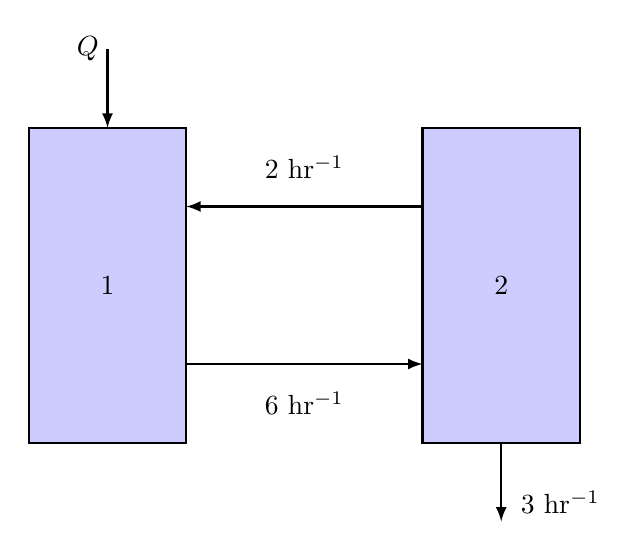
\begin{tikzpicture}
  \draw[thick,fill=blue!20]  (0,0) --  (0,4) -- (2,4) -- (2,0) -- cycle;
  \node at (1,2) {\circled{1}};  
  \draw[-latex,thick] (2,1) -- (5,1);
  \node at (3.5,0.5) {6~hr$^{-1}$};
  \draw[-latex,thick] (5,3) -- (2,3);
  \node at (3.5,3.5) {2~hr$^{-1}$};
  \draw[-latex,thick] (1,5) -- (1,4);
  \node at (0.75,5) {$Q$};
%%%%
  \draw[thick,fill=blue!20]  (5,0) --  (5,4) -- (7,4) -- (7,0) -- cycle;  
  \node at (6,2) {\circled{2}}; 
  \draw[-latex,thick] (6,0) -- (6,-1);
  \node at (6.75,-0.75) {3~hr$^{-1}$};
\end{tikzpicture}
\caption{Mass flow in solution tank example.}
\label{Fig:ode_massFlowExample}
\end{center}
\end{figure}

%%%%%%%%%%%%%%%%%%%%%%%%%%%%%%%%%%%%%%%%%%%%%%%%%%%%%%%%%%%%%%%%%%%%%%%%%%%%%%%%%%%%%%%%%%%%%%%
\subsection{Example: Mass Flow in Solution Tanks}

Suppose there are two interconnected solution tanks containing some fluid as depicted in Fig.~\ref{Fig:ode_massFlowExample}. Tank 1 drains into tank 2. Tank 2 can drain back into tank 1 as well as draining to the outside. At time $t = 0$, there are initially masses $m_1(0)$ and $m_2(0)$ in tanks 1 and 2 respectively. The rate of drainage from each tank is proportional to the mass fluid in each of the tanks. The drainage constant out of tank 1 into tank 2 is 6~hr$^{-1}$, the drainage constant out of tank 2 and back into tank 1 is 2~hr$^{-1}$, and the drainage constant out of tank 2 to the outside is 3~hr${}^{-1}$. Also, suppose that fluid is being added to tank 1 at a constant rate $Q$. Our goal is to find the mass of fluid in each tank at time $t$.

First, we write down the differential equations:
\begin{subequations}
\begin{align}
  &\frac{dm_1}{dt} = -6 m_1(t) + 2 m_2(t) + Q, \\*
  &\frac{dm_2}{dt} = (-2 - 3) m_2(t) + 6 m_1(t). 
\end{align}
\end{subequations}
Rearranging these into matrix-vector form gives:
\begin{align}
  \frac{d}{dt} \left[ \begin{array}{c} m_1(t) \\ m_2(t) \\ \end{array} \right]
  + \left[ \begin{array}{r r}
   6 & -2 \\
  -6 &  5 \\ \end{array} \right]
  \left[ \begin{array}{c} m_1(t) \\ m_2(t) \\ \end{array} \right]
  + \left[ \begin{array}{c} Q \\ 0 \\ \end{array} \right] .
\end{align}
To diagonalize this system, we must find the eigenvalues and eigenvectors of the matrix
\begin{align}
  \mathbf{A} = \left[ \begin{array}{r r}
   6 & -2 \\
  -6 &  5 \\ \end{array} \right].
\end{align}
These are:
\begin{align}
  \lambda = \left\{ 2, 9 \right\}; 
  \quad \mathbf{v} = \left\{  
  \left[ \begin{array}{r}  1 \\ 2 \\ \end{array} \right] ,
  \left[ \begin{array}{r} -2 \\ 3 \\ \end{array} \right] \right\} .
\end{align}
The transformation matrix contains the eigenvectors as its columns:
\begin{align}
  \mathbf{T} = \left[ \begin{array}{r r}
   1 & -2 \\
   2 &  3 \\ \end{array} \right] . 
\end{align}
The diagonal matrix $\mathbf{D}$ has the corresponding eigenvalues as its elements:
\begin{align}
  \mathbf{D} = \left[ \begin{array}{r r}
   2 &  0 \\
   0 &  9 \\ \end{array} \right] . 
\end{align}
Now we find the initial conditions $\mathbf{z}(0)$ and the inhomogeneous term $\mathbf{r}(t)$ in the transformed coordinates. Since the system is only 2$\times$2 we can compute its inverse simply as
\begin{align}
  \mathbf{T}^{-1} = \frac{1}{7} \left[ \begin{array}{r r}
   3 &  2 \\
  -2 &  1 \\ \end{array} \right] . 
\end{align}
We can then compute these as
\begin{align}
  &\mathbf{z}(0) = \mathbf{T}^{-1} \mathbf{m}(0) 
  = \frac{1}{7} \left[ \begin{array}{r r}
   3 &  2 \\
  -2 &  1 \\ \end{array} \right]
  \left[ \begin{array}{c} m_1(0) \\ m_2(0) \\ \end{array} \right]
  = \frac{1}{7} \left[ \begin{array}{c} 3 m_1(0) + 2 m_2(0) \\ -2 m_1(0) + m_2(0) \\ \end{array} \right] , \\
%%%%%
  &\mathbf{r}(t) = \mathbf{T}^{-1} \mathbf{q}(t) 
  = \frac{1}{7} \left[ \begin{array}{r r}
   3 &  2 \\
  -2 &  1 \\ \end{array} \right]
  \left[ \begin{array}{c} Q \\ 0 \\ \end{array} \right]
  = \frac{Q}{7} \left[ \begin{array}{c} 3 \\ -2 \\ \end{array} \right] .
\end{align}
The solution is
\begin{align}
  \mathbf{m}(t) 
  &= \left[ \frac{1}{7} (  3 m_1(0) + 2 m_2(0) ) e^{-2t} + \frac{3Q}{7} \int_0^t e^{-2(t-t')} dt' \right] \left[ \begin{array}{r}  1 \\ 2 \\ \end{array} \right] \nonumber \\*
  &+ \left[ \frac{1}{7} ( -2 m_1(0) +   m_2(0) ) e^{-9t} - \frac{2Q}{7} \int_0^t e^{-9(t-t')} dt' \right] \left[ \begin{array}{r} -2 \\ 3 \\ \end{array} \right] .
\end{align}
Carrying out the integrals gives
\begin{align}
  \mathbf{m}(t) 
  &= \left[ \frac{1}{7} (  3 m_1(0) + 2 m_2(0) ) e^{-2t} + \frac{3Q}{14} ( 1 -  e^{-2t} ) \right] \left[ \begin{array}{r}  1 \\ 2 \\ \end{array} \right] \nonumber \\*
  &+ \left[ \frac{1}{7} ( -2 m_1(0) +   m_2(0) ) e^{-9t} - \frac{2Q}{63} ( 1 -  e^{-9t} ) \right] \left[ \begin{array}{r} -2 \\ 3 \\ \end{array} \right] .
\end{align}
Writing out the equations explicitly:
\begin{subequations}
\begin{align}
  m_1(t) &= m_1(0) \left( \frac{3}{7} e^{-2t} + \frac{4}{7} e^{-9t} \right) 
          + m_2(0) \left( \frac{2}{7} e^{-2t} - \frac{2}{7} e^{-9t} \right) \nonumber \\*
         &+ \frac{3Q}{14} ( 1 -  e^{-2t} ) + \frac{4Q}{63} ( 1 -  e^{-9t} ) , \\
  m_2(t) &= m_1(0) \left( \frac{6}{7} e^{-2t} - \frac{6}{7} e^{-9t} \right)
          + m_2(0) \left( \frac{4}{7} e^{-2t} + \frac{3}{7} e^{-9t} \right) \nonumber \\*
         &+ \frac{3Q}{7} ( 1 -  e^{-2t} ) + \frac{4Q}{21} ( 1 -  e^{-9t} ) .
\end{align}
\end{subequations}

%%%%%%%%%%%%%%%%%%%%%%%%%%%%%%%%%%%%%%%%%%%%%%%%%%%%%%%%%%%%%%%%%%%%%%%%%%%%%%%%%%%%%%%%%%%%%%%
\subsection{Complex Eigenvalues} \label{Sec:ode_diagonalization_complexEigenvalues}

In many situations, the eigenvalues are complex, $\lambda = a + bi$ with $i = \sqrt{-1}$, the imaginary unit. The formulas used before are still valid, however, one additional piece of information is the Euler formula
\begin{align}
  e^{i\theta} = \cos \theta + i \sin \theta,
\end{align}
which relates the exponential of an imaginary number to trigonometric functions. This implies complex eigenvalues have oscillatory behavior. If the coefficients are all real, then we can assert that if an eigenvalue is complex $a + bi$, then its complex conjugate $a - bi$ is also an eigenvalue. The same can said of the corresponding eigenvectors. In these cases, the mathematics will work out so that the solution is entirely real.

Let us illustrate with an example:
\begin{align}
  \mathbf{y}'(t) + \left[ \begin{array}{r r r}
   4 &  0 &  0 \\
  -4 &  1 &  1 \\
   0 & -1 &  1 \\ \end{array} \right] \mathbf{y}(t) = \mathbf{0}, \quad 
   \mathbf{y}(0) = \left[ \begin{array}{c} 1 \\ 0 \\ 0 \\ \end{array} \right] .
\end{align}
The eigenvalues and eigenvectors of this matrix are:
\begin{align}
  \lambda = \left\{ 4, 1 + i, 1 - i \right\}; \quad
  \mathbf{v} = \left\{ 
  \left[ \begin{array}{c} 5 \\ -6 \\ 2 \\ \end{array} \right],
  \left[ \begin{array}{c} 0 \\ -i \\ 1 \\ \end{array} \right],
  \left[ \begin{array}{c} 0 \\  i \\ 1 \\ \end{array} \right] \right\}  .
\end{align}
The transformation matrix is therefore:
\begin{align}
  \mathbf{T} = \left[ \begin{array}{r r r}
   5 &  0 &  0 \\
  -6 & -i &  i \\
   2 &  1 &  1 \\ \end{array} \right] .
\end{align}
The equation is homogeneous, so we only have the initial condition in the transformed coordinate. This can be obtained by solving
\begin{align}
  \mathbf{T} \mathbf{z}(0) = \mathbf{y}(0) \nonumber
\end{align}
to obtain
\begin{align}
  \mathbf{z}(0) = \frac{1}{5} \left[ \begin{array}{c} 1 \\ -1 + 3i \\ -1 - 3i \\ \end{array} \right] .
\end{align}
The solution is therefore
\begin{align}
  \mathbf{y}(t) = \frac{1}{5} e^{-4t} \left[ \begin{array}{c} 5 \\ -6 \\ 2 \\ \end{array} \right]
                &+ \frac{1}{5} ( -1 + 3i ) e^{-(1+i)t} \left[ \begin{array}{c} 0 \\ -i \\ 1 \\ \end{array} \right] \nonumber \\*
                &+ \frac{1}{5} ( -1 - 3i ) e^{-(1-i)t} \left[ \begin{array}{c} 0 \\  i \\ 1 \\ \end{array} \right] .
\end{align}
Applying Euler's formula to the complex exponential gives
\begin{align}
  \mathbf{y}(t) = \frac{1}{5} e^{-4t} \left[ \begin{array}{c} 5 \\ -6 \\ 2 \\ \end{array} \right]
                &+ \frac{1}{5} ( -1 + 3i ) e^{-t} ( \cos(t) - i \sin(t) ) \left[ \begin{array}{c} 0 \\ -i \\ 1 \\ \end{array} \right] \nonumber \\*
                &+ \frac{1}{5} ( -1 - 3i ) e^{-t} ( \cos(t) + i \sin(t) ) \left[ \begin{array}{c} 0 \\  i \\ 1 \\ \end{array} \right] .
\end{align}
Writing each of these out explicitly:
\begin{subequations}
\begin{align}
  y_1(t) &= e^{-4t}, \\
  y_2(t) &= -\frac{6}{5} e^{-4t} + \frac{1}{5} ( 3 + i ) e^{-t} ( \cos(t) - i \sin(t) ) \nonumber \\ &\hspace{1.9cm} + \frac{1}{5} ( 3 - i ) e^{-t} ( \cos(t) + i \sin(t) ) \nonumber \\*
         &= -\frac{6}{5} e^{-4t} + \left( \frac{6}{5} \cos(t) + \frac{2}{5} \sin(t) \right) e^{-t}, \\
  y_3(t) &=  \frac{2}{5} e^{-4t} + \frac{1}{5} (-1 + 3i) e^{-t} ( \cos(t) - i \sin(t) ) \nonumber \\ &\hspace{1.5cm} + \frac{1}{5} (-1 - 3i) e^{-t} ( \cos(t) + i \sin(t) ) \nonumber \\*
         &=  \frac{2}{5} e^{-4t} + \left( -\frac{2}{5} \cos(t) + \frac{6}{5} \sin(t) \right) e^{-t}.
\end{align}
\end{subequations}
The solution for $y_1(t)$ is pure exponential decay. The solutions for $y_2(t)$ and $y_3(t)$ are damped oscillations. Note the key point that despite imaginary values showing up in the intermediate steps, the solution is indeed real. This will always be the case if the coefficients are entirely real.

%%%%%%%%%%%%%%%%%%%%%%%%%%%%%%%%%%%%%%%%%%%%%%%%%%%%%%%%%%%%%%%%%%%%%%%%%%%%%%%%%%%%%%%%%%%%%%%
\subsection{Defective Matrices}

As we saw in the last chapter, sometimes a system can have repeated eigenvalues, which may also have fewer linearly independent eigenvectors than the number of unknowns. This case may also arise in the context of systems of ODEs. What this means is the matrix cannot be diagonalized. Thankfully, this situation seldom arises in engineering applications, so it will only be mentioned briefly here.

When this occurs, we need to find additional information in the form of \emph{generalized eigenvectors}. This is obtained from successive application of the operator $\mathbf{A} - \lambda \mathbf{I}$. Suppose $\mathbf{v}_1$ is the only linearly independent eigenvector for a particular eigenvalue. The generalized eigenvectors may be obtained from
\begin{align}
  ( \mathbf{A} - \lambda \mathbf{I} ) \mathbf{v}_1 &= \mathbf{0}, \nonumber \\
  ( \mathbf{A} - \lambda \mathbf{I} ) \mathbf{v}_2 &= \mathbf{v}_1, \nonumber \\
  ( \mathbf{A} - \lambda \mathbf{I} ) \mathbf{v}_3 &= \mathbf{v}_2,  \nonumber \\
  &\vdots    \nonumber
\end{align}
Using these generalized eigenvectors to form a transformation matrix $\mathbf{T}$ yields an almost diagonalized matrix with a \emph{Jordan normal form} where the matrix is diagonal with the exception of values of 1 that appear on the superdiagonal where eigenvalues with multiplicity and fewer linearly independent eigenvectors occur. When taking the matrix exponential of such a matrix, we end up with exponentials with polynomial coefficients $t, t^2, \ldots$ analogous to second-order ODEs for which the characteristic equation has a repeated root.



%%%%%%%%%%%%%%%%%%%%%%%%%%%%%%%%%%%%%%%%%%%%%%%%%%%%%%%%%%%%%%%%%%%%%%%%%%%%%%%%%%%%%%%%%%%%%%%%
%%%%%%%%%%%%%%%%%%%%%%%%%%%%%%%%%%%%%%%%%%%%%%%%%%%%%%%%%%%%%%%%%%%%%%%%%%%%%%%%%%%%%%%%%%%%%%%%
\section{Numerical Techniques} \label{Sec:ode_numericalTechniques}

The matrix exponential and diagonalization methods are only applicable if the ODE is linear and its coefficients are constant. In the cases where they are not, there is no general solution, and usually we revert to performing numerical approximation methods. This section introduces the techniques in the context of linear ODEs with coefficients that are functions of time. Following this, the techniques will be applied to systems of general first-order ODEs. 

A system of first-order ODEs may be written generically as
\begin{align}
  \mathbf{y}'(t) = \mathbf{f}( t, \mathbf{y}(t) ), \quad \mathbf{y}(0) = \mathbf{y}_0.
\end{align}
Here $\mathbf{f}$ is a vector because each equation could involve a different function $f_i(t,\mathbf{y}(t))$. For the first-order linear ODE this becomes
\begin{align}
  \mathbf{y}'(t) = -\mathbf{P}(t) \mathbf{y}(t) + \mathbf{q}(t), \quad \mathbf{y}(0) = \mathbf{y}_0,
\end{align}
where $\mathbf{P}(t)$ is a general function of time, this system has no analytical solution; however, we could approximate the solution on a time grid: $t_0 = 0, t_1 = \Delta t_1, t_2 = t_1 + \Delta t_2, \ldots$ In most cases, $\Delta t_n$ will be a fixed interval $\Delta t$ so that $t_0 = 0, t_1 = \Delta t, t_2 = 2 \Delta t, \ldots$  While not necessary, this simplifies the coding as well as the mathematical analysis. The equations herein will use a fixed $\Delta t$ for simplicity.

The first derivative may be approximated using the finite difference:
\begin{align}
  \mathbf{y}'(t) \approx \frac{1}{\Delta t} \left( \mathbf{y}(t_{n+1}) - \mathbf{y}(t_n) \right) = \frac{1}{\Delta t}  \left( \mathbf{y}_{n+1} - \mathbf{y}_n \right) .
\end{align}
Here we introduced the shorthand $\mathbf{y}(t_n) = \mathbf{y}_n$ to keep the notation compact. Now we must map the right-hand side of the equation onto the time grid. There are different options for doing this that have implications on how well the solution is approximated as well as whether the numerical method converges at all. These notes will discuss the three elementary techniques: forward Euler, backward Euler, and improved Euler or the trapezoidal rule.

%%%%%%%%%%%%%%%%%%%%%%%%%%%%%%%%%%%%%%%%%%%%%%%%%%%%%%%%%%%%%%%%%%%%%%%%%%%%%%%%%%%%%%%%%%%%%%%%
\subsection{Forward Euler}

The forward Euler method takes the right-hand side at the left endpoint of the current time interval. After the finite difference is applied to the first derivative, the system can be written as
\begin{align}
   \frac{1}{\Delta t}  \left( \mathbf{y}_{n+1} - \mathbf{y}_n \right) = \mathbf{f}( t_n, \mathbf{y}_n ).
\end{align}
Solving for $\mathbf{y}_{n+1}$ is straightforward:
\begin{align}
  \mathbf{y}_{n+1} = \mathbf{y}_n + \Delta t \mathbf{f}( t_n, \mathbf{y}_n ).
\end{align}
For the linear ODE, this becomes
\begin{align}
  \mathbf{y}_{n+1} = \mathbf{y}_n + \Delta t \left( -\mathbf{P}_n \mathbf{y}_n + \mathbf{q}_n \right).
\end{align}
Factoring out $\mathbf{y}_n$ to the right on the right-hand side gives the final result:
\begin{align}
  \mathbf{y}_{n+1} = \left( \mathbf{I} - \Delta t \mathbf{P}_n \right) \mathbf{y}_n  + \Delta t \mathbf{q}_n.
\end{align}

The forward Euler method is advantageous because of its simplicity. Computing the approximate scheme simply involves doing a matrix multiplication at each time step and adding on the inhomogeneous term. Forward Euler is classified as an \emph{explicit method} in that the right-hand side of the original is completely known and therefore the solution at the next time step may be computed directly.

Unfortunately, forward Euler has a couple significant issues limiting its usefulness. The first issue is related to its convergence rate. The error incurred in the solution is proportional to the size of the time step $\Delta t$. It is often the case that to get suitable accuracy, one needs to take unacceptably small time steps. The other major issue with forward Euler is how the errors tend to compound. If $\Delta t$ is too large, we can get into a situation where the errors tend to geometrically grow with time. This means the solution becomes progressively worse with time until the solution ``blows up''. We say that the forward Euler method has the potential to become unstable if the time step is too large.

To illustrate some of these issues, let us consider the example from Sec.~\ref{Sec:ode_diagonalization_complexEigenvalues}. There we had the linear system:
\begin{align}
  \mathbf{y}'(t) + \left[ \begin{array}{r r r}
   4 &  0 &  0 \\
  -4 &  1 &  1 \\
   0 & -1 &  1 \\ \end{array} \right] \mathbf{y}(t) = \mathbf{0}, \quad 
   \mathbf{y}(0) = \left[ \begin{array}{c} 1 \\ 0 \\ 0 \\ \end{array} \right] , \nonumber
\end{align}
and worked out the solution. For illustration purposes, let us compare against the reference solution $y_2(t)$, which is
\begin{align}
  y_2(t) &= -\frac{6}{5} e^{-4t} + \left( \frac{6}{5} \cos(t) + \frac{2}{5} \sin(t) \right) e^{-t}. \nonumber
\end{align}
We may use forward Euler to approximate the solution as follows:
\begin{align}
  \left[ \begin{array}{c} y_{1,n+1} \\ y_{2,n+1} \\ y_{3,n+1} \end{array} \right] =
  \left[ \begin{array}{r r r}
   1 - 4\Delta t &             0 &             0 \\
       4\Delta t &  1 - \Delta t &     -\Delta t \\
               0 &      \Delta t &  1 - \Delta t \\ \end{array} \right]  
  \left[ \begin{array}{c} y_{1,n} \\ y_{2,n} \\ y_{3,n} \end{array} \right] .
\end{align}

\begin{figure}[htb!]
\begin{center}
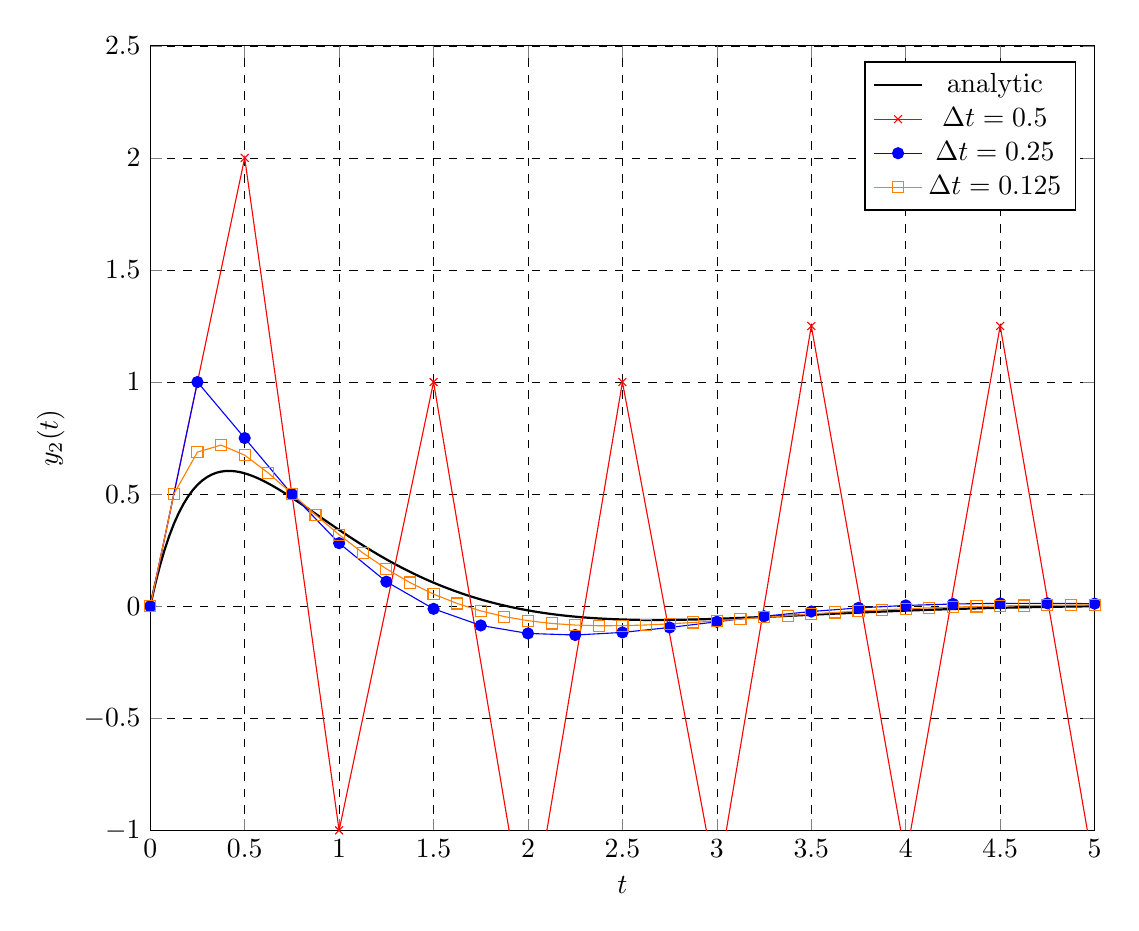
\begin{tikzpicture} \begin{axis}
[scale=1.75,
 xmin=0,    xmax=5,
 ymin=-1, ymax=2.5,
 grid=major, 
 major grid style={color=black,line width=0.2pt, dashed},
 xlabel=$t$,
 ylabel=$y_2(t)$,
]
\addplot[
   black,
   domain=0:5,
   samples=201,
   line width=0.8pt
]
{-1.2*exp(-4*x) + ( 1.2*cos(deg(x)) + 0.4*sin(deg(x)) )*exp(-x)};
\addlegendentry{analytic}

\addplot[color=red,mark=x] coordinates {
 ( 0 , 0 ) 
 ( 0.5 , 2 ) 
 ( 1 , -1 )
 ( 1.5 , 1 ) 
 ( 2 , -1.5 )
 ( 2.5 , 1 ) 
 ( 3 , -1.25 )
 ( 3.5 , 1.25 )
 ( 4 , -1.125 )
 ( 4.5 , 1.25 )
 ( 5 , -1.1875 )
};
\addlegendentry{$\Delta t = 0.5$}
\addplot[color=blue,mark=*] coordinates {
 ( 0 , 0 ) 
 ( 0.25 , 1 ) 
 ( 0.5 , 0.75 )
 ( 0.75 , 0.5 )
 ( 1 , 0.28125 )
 ( 1.25 , 0.109375 )
 ( 1.5 , -0.0117188 )
 ( 1.75 , -0.0859375 )
 ( 2 , -0.121582 )
 ( 2.25 , -0.128662 )
 ( 2.5 , -0.117004 )
 ( 2.75 , -0.0950928 )
 ( 3 , -0.0695114 )
 ( 3.25 , -0.0448341 )
 ( 3.5 , -0.0238066 )
 ( 3.75 , -0.00768852 )
 ( 4 , 0.00334632 )
 ( 4.25 , 0.00982481 )
 ( 4.5 , 0.0126458 )
 ( 4.75 , 0.0128281 )
 ( 5 , 0.0113386 )
};
\addlegendentry{$\Delta t = 0.25$}
\addplot[color=orange,mark=square] coordinates {
 ( 0 , 0 )
 ( 0.125 , 0.5 )
 ( 0.25 , 0.6875 )
 ( 0.375 , 0.71875 )
 ( 0.5 , 0.673828 )
 ( 0.625 , 0.594238 )
 ( 0.75 , 0.50177 )
 ( 0.875 , 0.40799 )
 ( 1 , 0.319044 )
 ( 1.125 , 0.238121 )
 ( 1.25 , 0.166725 )
 ( 1.375 , 0.105371 )
 ( 1.5 , 0.0539628 )
 ( 1.625 , 0.0120218 )
 ( 1.75 , -0.021166 )
 ( 1.875 , -0.0464554 )
 ( 2 , -0.0647725 )
 ( 2.125 , -0.0770643 )
 ( 2.25 , -0.0842619 )
 ( 2.375 , -0.0872532 )
 ( 2.5 , -0.0868642 )
 ( 2.625 , -0.0838462 )
 ( 2.75 , -0.0788684 )
 ( 2.875 , -0.0725149 )
 ( 3 , -0.0652852 )
 ( 3.125 , -0.0575968 )
 ( 3.25 , -0.0497904 )
 ( 3.375 , -0.0421357 )
 ( 3.5 , -0.0348387 )
 ( 3.625 , -0.0280493 )
 ( 3.75 , -0.0218685 )
 ( 3.875 , -0.0163563 )
 ( 4 , -0.0115388 )
 ( 4.125 , -0.00741454 )
 ( 4.25 , -0.00396076 )
 ( 4.375 , -0.00113872 )
 ( 4.5 , 0.00110159 )
 ( 4.625 , 0.0028174 )
 ( 4.75 , 0.00406984 )
 ( 4.875 , 0.00492112 )
 ( 5 , 0.0054324 )
};
\addlegendentry{$\Delta t = 0.125$}
\end{axis}
\end{tikzpicture}
\caption{Example of the forward Euler method.}
 \label{Fig:ode_forwardEulerExample}
\end{center}
\end{figure}

Let us consider the time interval $0 \le t \le 5$, with 10, 20, and 40 time intervals having $\Delta t = 0.5, 0.25, 0.125$ respectively. The analytic solution is compared with that obtained from the forward Euler method for various time steps in Fig.~\ref{Fig:ode_forwardEulerExample}. The analytical solution is plotted as the black smooth curve. The red line is for $\Delta t = 0.5$. This line is very jagged and oscillates wildly. It does not approximate the solution well at all. This is a consequence of the time step being too large and the errors growing. The blue curve gives the result for $\Delta t = 0.25$. This curve does not exhibit the large oscillations, and is somewhat representative of the shape of the analytical solution. The orange curve gives the result for $\Delta t = 0.125$. This curve is closer to the analytical solution. Indeed, if $\Delta t$ is made increasingly small, the result will approach the actual analytical solution.


%%%%%%%%%%%%%%%%%%%%%%%%%%%%%%%%%%%%%%%%%%%%%%%%%%%%%%%%%%%%%%%%%%%%%%%%%%%%%%%%%%%%%%%%%%%%%%%%
\subsection{Backward Euler}

An alternative is to take the right-hand side at the right endpoint of the time interval:
\begin{align}
   \frac{1}{\Delta t}  \left( \mathbf{y}_{n+1} - \mathbf{y}_n \right) = \mathbf{f}( t_{n+1}, \mathbf{y}_{n+1} ).
\end{align}
For the linear ODE this becomes
\begin{align}
   \frac{1}{\Delta t}  \left( \mathbf{y}_{n+1} - \mathbf{y}_n \right) = -\mathbf{P}_{n+1} \mathbf{y}_{n+1} + \mathbf{q}_{n+1} .
\end{align}
Moving the $\mathbf{y}$ terms at time step $n$ to the right-hand side and $n+1$ terms to the left-hand side gives:
\begin{align}
   \mathbf{y}_{n+1} + \Delta t \mathbf{P}_{n+1} \mathbf{y}_{n+1} = \mathbf{y}_n + \Delta t \mathbf{q}_{n+1} .
\end{align}
Factoring the left-hand side gives the linear system for the unknown value of $\mathbf{y}$ at the following time step:
\begin{align}
   \left( \mathbf{I} + \Delta t \mathbf{P}_{n+1} \right) \mathbf{y}_{n+1} = \mathbf{y}_n + \Delta t \mathbf{q}_{n+1} .
\end{align}
The linear system is solved using various techniques of linear algebra, e.g., Gaussian elimination.

The backward Euler scheme has a significant addition in complexity over forward Euler in that there is now a linear system of equations to solve. This is a consequence of the right-hand side being taken at the following time step. We call this an \emph{implicit method} in that we need to simultaneously solve for the right-hand side and the solution vector.

As with forward Euler, the backward Euler scheme has an error that is proportional to the size of the time step $\Delta t$. Backward Euler does, however, have one major advantage over forward Euler. The errors that occur during each time step tend to offset each time step and cancel one another out, which implies that the error terms will dampen with time. If time steps are too large, then we will observe false oscillatory behavior each time step indicative of this trend.

\begin{figure}[tb!]
\begin{center}
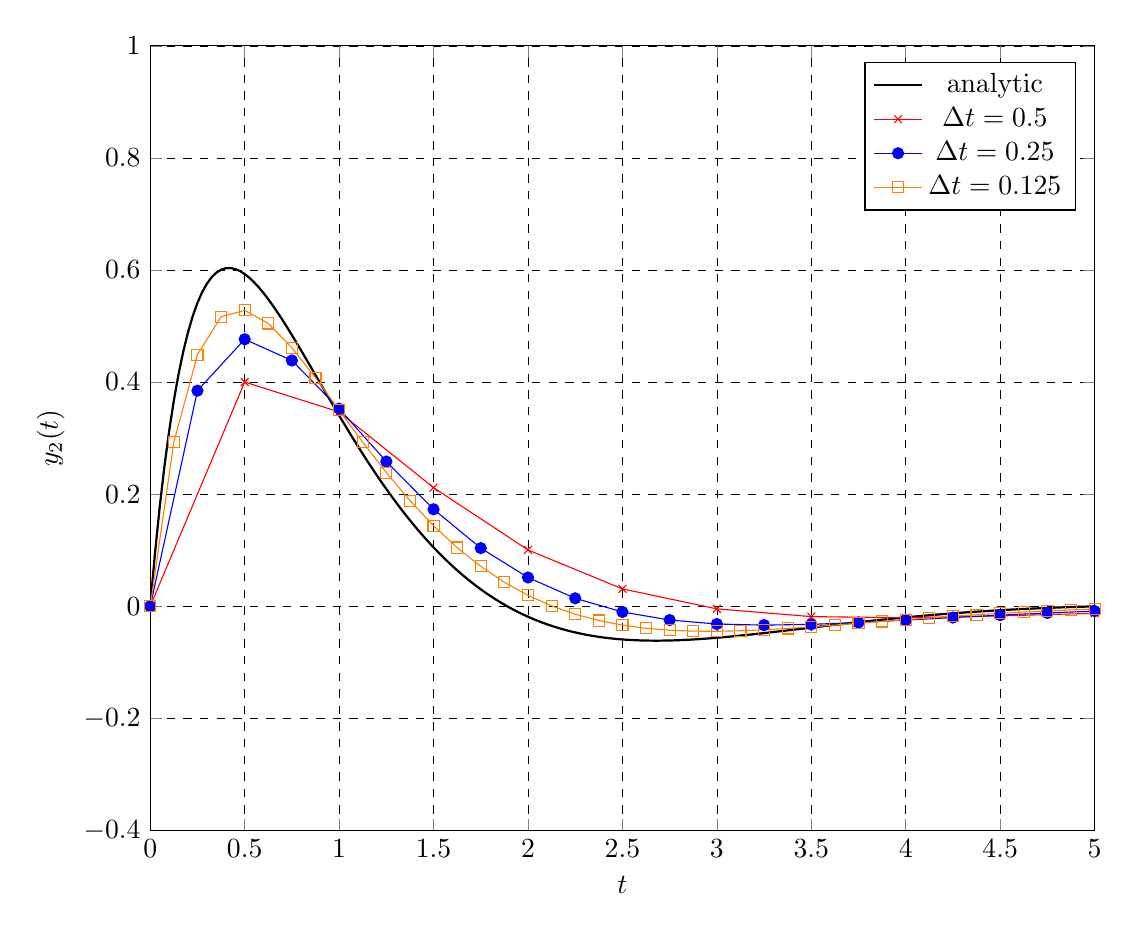
\begin{tikzpicture} \begin{axis}
[scale=1.75,
 xmin=0,    xmax=5,
 ymin=-0.4, ymax=1.0,
 grid=major, 
 major grid style={color=black,line width=0.2pt, dashed},
 xlabel=$t$,
 ylabel=$y_2(t)$,
]
\addplot[
   black,
   domain=0:5,
   samples=201,
   line width=0.8pt
]
{-1.2*exp(-4*x) + ( 1.2*cos(deg(x)) + 0.4*sin(deg(x)) )*exp(-x)};
\addlegendentry{analytic}

\addplot[color=red,mark=x] coordinates {
 ( 0 , 0 ) 
 ( 0.5 , 0.4 )
 ( 1 , 0.346667 )
 ( 1.5 , 0.211556 )
 ( 2 , 0.100385 )
 ( 2.5 , 0.0309017 )
 ( 3 , -0.00471809 )
 ( 3.5 , -0.0185711 )
 ( 4 , -0.020581 )
 ( 4.5 , -0.0173297 )
 ( 5 , -0.0125836 )
};
\addlegendentry{$\Delta t = 0.5$}
\addplot[color=blue,mark=*] coordinates {
 ( 0 , 0 ) 
 ( 0.25 , 0.384615 )
 ( 0.5 , 0.476331 )
 ( 0.75 , 0.438439 )
 ( 1 , 0.352548 )
 ( 1.25 , 0.25815 )
 ( 1.5 , 0.17299 )
 ( 1.75 , 0.103671 )
 ( 2 , 0.0512353 )
 ( 2.25 , 0.0141248 )
 ( 2.5 , -0.0102498 )
 ( 2.75 , -0.0246864 )
 ( 3 , -0.0317842 )
 ( 3.25 , -0.0337635 )
 ( 3.5 , -0.0324125 )
 ( 3.75 , -0.0291019 )
 ( 4 , -0.0248331 )
 ( 4.25 , -0.0202994 )
 ( 4.5 , -0.0159497 )
 ( 4.75 , -0.0120469 )
 ( 5 , -0.00871898 )
};
\addlegendentry{$\Delta t = 0.25$}
\addplot[color=orange,mark=square] coordinates {
 ( 0 , 0 ) 
 ( 0.125 , 0.292683 )
 ( 0.25 , 0.448939 )
 ( 0.375 , 0.516585 )
 ( 0.5 , 0.527875 )
 ( 0.625 , 0.504541 )
 ( 0.75 , 0.461175 )
 ( 0.875 , 0.407516 )
 ( 1 , 0.349985 )
 ( 1.125 , 0.292741 )
 ( 1.25 , 0.238385 )
 ( 1.375 , 0.188454 )
 ( 1.5 , 0.14376 )
 ( 1.625 , 0.104618 )
 ( 1.75 , 0.071015 )
 ( 1.875 , 0.0427223 )
 ( 2 , 0.0193753 )
 ( 2.125 , 0.00053222 )
 ( 2.25 , -0.0142866 )
 ( 2.375 , -0.0255701 )
 ( 2.5 , -0.033797 )
 ( 2.625 , -0.0394231 )
 ( 2.75 , -0.0428722 )
 ( 2.875 , -0.0445315 )
 ( 3 , -0.0447492 )
 ( 3.125 , -0.0438334 )
 ( 3.25 , -0.0420534 )
 ( 3.375 , -0.039641 )
 ( 3.5 , -0.0367931 )
 ( 3.625 , -0.033674 )
 ( 3.75 , -0.0304191 )
 ( 3.875 , -0.0271372 )
 ( 4 , -0.0239142 )
 ( 4.125 , -0.0208157 )
 ( 4.25 , -0.0178897 )
 ( 4.375 , -0.0151699 )
 ( 4.5 , -0.0126771 )
 ( 4.625 , -0.0104224 )
 ( 4.75 , -0.00840839 )
 ( 4.875 , -0.00663146 )
 ( 5 , -0.00508285 )
};
\addlegendentry{$\Delta t = 0.125$}
\end{axis}
\end{tikzpicture}
\caption{Example of the backward Euler method.}
 \label{Fig:ode_backwardEulerExample}
\end{center}
\end{figure}

The same example that was used for forward Euler is solved again, but this time with backward Euler. The linear system  solved is
\begin{align}
  \left[ \begin{array}{r r r}
   1 + 4\Delta t &             0 &             0 \\
      -4\Delta t &  1 + \Delta t &      \Delta t \\
               0 &     -\Delta t &  1 + \Delta t \\ \end{array} \right]  
  \left[ \begin{array}{c} y_{1,n+1} \\ y_{2,n+1} \\ y_{3,n+1} \end{array} \right] =
  \left[ \begin{array}{c} y_{1,n} \\ y_{2,n} \\ y_{3,n} \end{array} \right] .
\end{align}
The results are given in Fig.~\ref{Fig:ode_backwardEulerExample}. This time the $\Delta t = 0.5$ solution follows the general shape of the solution and, unlike forward Euler, does not wildly oscillate. This is because of the fact that backward Euler has increased stability. The level of agreement otherwise is about the same for forward and backward Euler, which is to be expected as they have the same rate of error decay.

%%%%%%%%%%%%%%%%%%%%%%%%%%%%%%%%%%%%%%%%%%%%%%%%%%%%%%%%%%%%%%%%%%%%%%%%%%%%%%%%%%%%%%%%%%%%%%%%
\subsection{Improved Euler (Trapezoidal Rule)}

Previously, we discussed the explicit forward Euler scheme as well as the backward Euler scheme. Both of these methods have an error proportional to the width of the time step $\Delta t$. It reasons to ask whether one could devise a scheme that can converge more rapidly with the time step. The answer to this is yes, and the simplest approach is based on the trapezoidal rule called improved Euler. This takes the right-hand side at the midpoint of the time interval using the arithmetic mean:
\begin{align}
   \frac{1}{\Delta t}  \left( \mathbf{y}_{n+1} - \mathbf{y}_n \right) = \frac{1}{2} \left[ \mathbf{f}( t_n, \mathbf{y}_n ) + \mathbf{f}( t_{n+1}, \mathbf{y}_{n+1} ) \right].
\end{align}
As before, we bring all of the terms for $\mathbf{y}_{n+1}$ to the left-hand side and everything else to the right-hand side. After factoring, the expression becomes
\begin{align}
  \left( \mathbf{I} + \frac{\Delta t}{2} \mathbf{P}_{n+1} \right) \mathbf{y}_{n+1} = 
  \left( \mathbf{I} - \frac{\Delta t}{2} \mathbf{P}_{n}   \right) \mathbf{y}_n + \frac{\Delta t}{2} \left( \mathbf{q}_n + \mathbf{q}_{n+1} \right) .
\end{align}

As with backward Euler, we must solve a linear system of equations to obtain the solution, making this another implicit scheme. While more complicated than both forward and backward Euler, the trapezoidal rule has two very attractive properties. First, the error converges as $(\Delta t)^2$, meaning that as the time step gets smaller, the error gets smaller at a much faster rate. Second, like backward Euler, the error terms tend to offset and dampen with time, leading to an algorithm that is stable.

\begin{figure}[tb!]
\begin{center}
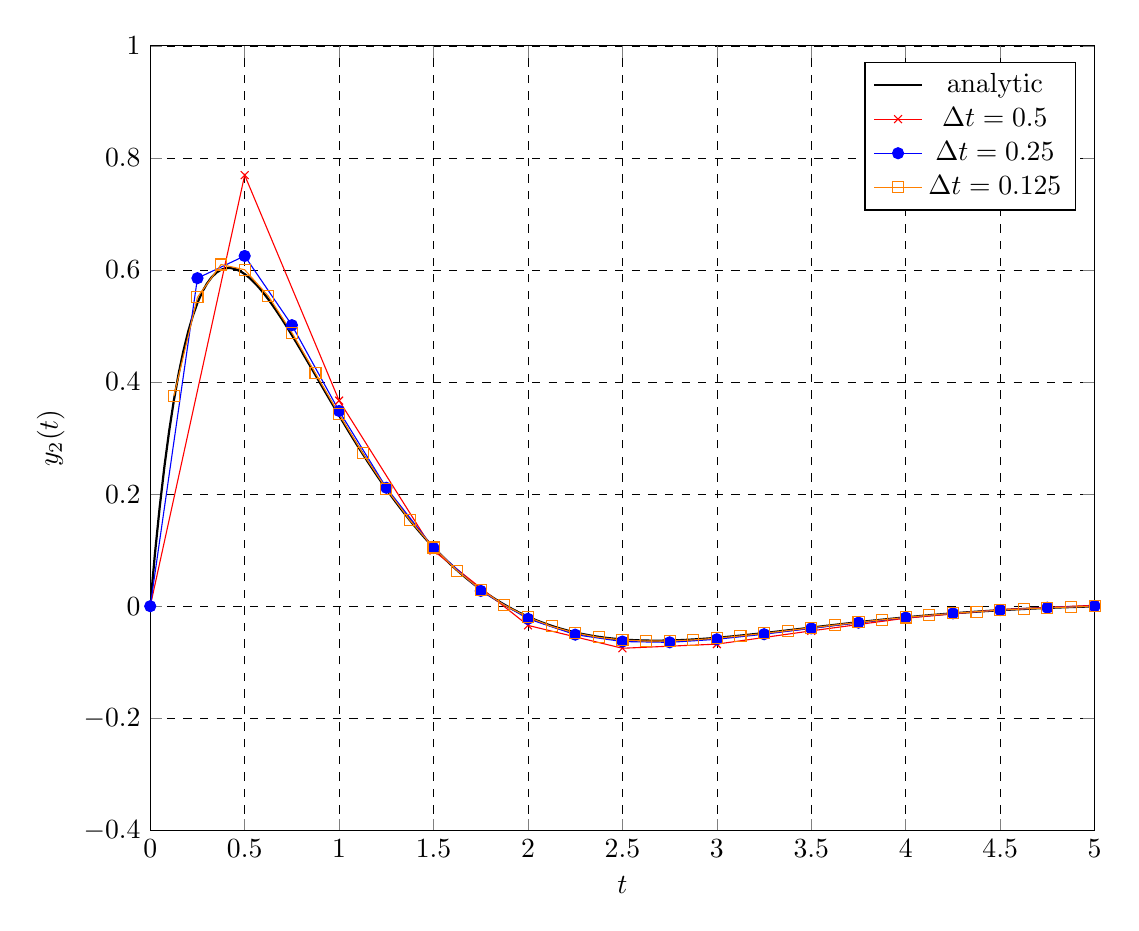
\begin{tikzpicture} \begin{axis}
[scale=1.75,
 xmin=0,    xmax=5,
 ymin=-0.4, ymax=1.0,
 grid=major, 
 major grid style={color=black,line width=0.2pt, dashed},
 xlabel=$t$,
 ylabel=$y_2(t)$,
]
\addplot[
   black,
   domain=0:5,
   samples=201,
   line width=0.8pt
]
{-1.2*exp(-4*x) + ( 1.2*cos(deg(x)) + 0.4*sin(deg(x)) )*exp(-x)};
\addlegendentry{analytic}

\addplot[color=red,mark=x] coordinates {
 ( 0 , 0 ) 
 ( 0.5 , 0.769231 )
 ( 1 , 0.366864 )
 ( 1.5 , 0.0992262 )
 ( 2 , -0.0342425 )
 ( 2.5 , -0.0750405 )
 ( 3 , -0.0676426 )
 ( 3.5 , -0.0439842 )
 ( 4 , -0.0213512 )
 ( 4.5 , -0.00607659 )
 ( 5 , 0.00166797 )
};
\addlegendentry{$\Delta t = 0.5$}
\addplot[color=blue,mark=*] coordinates {
 ( 0 , 0 ) 
 ( 0.25 , 0.585366 )
 ( 0.5 , 0.625025 )
 ( 0.75 , 0.501508 )
 ( 1 , 0.348359 )
 ( 1.25 , 0.211353 )
 ( 1.5 , 0.103981 )
 ( 1.75 , 0.0272953 )
 ( 2 , -0.0224841 )
 ( 2.25 , -0.0507628 )
 ( 2.5 , -0.0630931 )
 ( 2.75 , -0.0644693 )
 ( 3 , -0.0590232 )
 ( 3.25 , -0.0499455 )
 ( 3.5 , -0.0395381 )
 ( 3.75 , -0.0293349 )
 ( 4 , -0.0202516 )
 ( 4.25 , -0.0127372 )
 ( 4.5 , -0.00691261 )
 ( 4.75 , -0.00268664 )
 ( 5 , 0.000152288 )
};
\addlegendentry{$\Delta t = 0.25$}
\addplot[color=orange,mark=square] coordinates {
 ( 0.125 , 0.375172 )
 ( 0.25 , 0.551268 )
 ( 0.375 , 0.609734 )
 ( 0.5 , 0.600343 )
 ( 0.625 , 0.553581 )
 ( 0.75 , 0.48814 )
 ( 0.875 , 0.415438 )
 ( 1 , 0.342377 )
 ( 1.125 , 0.27303 )
 ( 1.25 , 0.209676 )
 ( 1.375 , 0.153452 )
 ( 1.5 , 0.104763 )
 ( 1.625 , 0.0635439 )
 ( 1.75 , 0.0294382 )
 ( 1.875 , 0.00190886 )
 ( 2 , -0.0196807 )
 ( 2.125 , -0.0360126 )
 ( 2.25 , -0.0477766 )
 ( 2.375 , -0.0556444 )
 ( 2.5 , -0.0602516 )
 ( 2.625 , -0.0621864 )
 ( 2.75 , -0.0619825 )
 ( 2.875 , -0.0601162 )
 ( 3 , -0.0570047 )
 ( 3.125 , -0.0530082 )
 ( 3.25 , -0.0484319 )
 ( 3.375 , -0.0435297 )
 ( 3.5 , -0.0385088 )
 ( 3.625 , -0.0335338 )
 ( 3.75 , -0.0287317 )
 ( 3.875 , -0.0241968 )
 ( 4 , -0.0199952 )
 ( 4.125 , -0.0161693 )
 ( 4.25 , -0.0127417 )
 ( 4.375 , -0.00971903 )
 ( 4.5 , -0.00709534 )
 ( 4.625 , -0.00485493 )
 ( 4.75 , -0.00297503 )
 ( 4.875 , -0.00142794 )
 ( 5 , -0.000182881 )
};
\addlegendentry{$\Delta t = 0.125$}
\end{axis}
\end{tikzpicture}
\caption{Example of the improved Euler method.}
 \label{Fig:ode_improvedEulerExample}
\end{center}
\end{figure}

The same example as with forward and backward Euler is repeated. This time the system of equations is 
\begin{align}
  \left[ \begin{array}{r r r}
   1 + 4( \rfrac{\Delta t}{2} ) &                            0 &                            0 \\
      -4( \rfrac{\Delta t}{2} ) &  1 + ( \rfrac{\Delta t}{2} ) &      ( \rfrac{\Delta t}{2} ) \\
                              0 &     -( \rfrac{\Delta t}{2} ) &  1 + ( \rfrac{\Delta t}{2} ) \\ \end{array} \right]  
  \left[ \begin{array}{c} y_{1,n+1} \\ y_{2,n+1} \\ y_{3,n+1} \end{array} \right] \nonumber \\
  =  \left[ \begin{array}{r r r}
   1 - 4( \rfrac{\Delta t}{2} ) &                            0 &                            0 \\
       4( \rfrac{\Delta t}{2} ) &  1 - ( \rfrac{\Delta t}{2} ) &     -( \rfrac{\Delta t}{2} ) \\
                              0 &      ( \rfrac{\Delta t}{2} ) &  1 - ( \rfrac{\Delta t}{2} ) \\ \end{array} \right]
  \left[ \begin{array}{c} y_{1,n} \\ y_{2,n} \\ y_{3,n} \end{array} \right] .
\end{align}
The results are shown in Fig.~\ref{Fig:ode_improvedEulerExample}. As with backward Euler, none of the results exhibit any serious problems seen for the forward Euler $\Delta t = 0.5$ case. The improved Euler method shows better convergence properties compared to both the forward and backward Euler, with even the $\Delta t = 0.5$ case showing good agreement except for early in the solution. This is consistent with the rate of decay of the error being proportional to $(\Delta t)^2$.

It is natural to ask whether one can get a faster convergence rate than $(\Delta t)^2$, and the answer is yes for both explicit and implicit methods. There are increasingly complicated methods with faster convergence rates. These methods are very powerful and used in practice, however, there is an important consideration regarding the stability of the solution method, i.e., whether or not the method will indeed converge. For linear ODEs the backward and improved Euler methods are guaranteed to be stable (nonlinear systems cannot necessarily guarantee this). Unfortunately, any method with a convergence rate of faster than $(\Delta t)^2$ is not unconditionally stable and care must be taken to ensure convergence. These more advanced methods could easily fill part of a numerical methods course and will not be explored here.

%%%%%%%%%%%%%%%%%%%%%%%%%%%%%%%%%%%%%%%%%%%%%%%%%%%%%%%%%%%%%%%%%%%%%%%%%%%%%%%%%%%%%%%%%%%%%%%%
\subsection{Error Comparisons}

The last few sections made assertions about the rate of convergence of the forward, backward, and improved Euler methods. The forward and backward Euler methods have an error that scales as $\Delta t$ and the improved Euler method has an error that scales as $(\Delta t)^2$. If the error goes as
\begin{align}
  \epsilon = c ( \Delta t )^k = c \left( \frac{T}{N} \right)^k \rightarrow \frac{c}{N^{k}} \nonumber,
\end{align}
where $c$ is some constant describing the magnitude of the error, $T$ is the time interval that the simulation is run that gets pulled into the constant, $N$ is the number of time steps, and $k$ is the convergence rate. It is illustrative to take the logarithm of both sides of the equation
\begin{align}
  \log \epsilon = \log c - k \log( N ). \nonumber
\end{align}
The base of the logarithm is not particularly relevant. This expression shows that the logarithm of the error is linear with respect to the logarithm of the number of time steps. The slope of the line is negative, $-k$, meaning the error should be inversely proportional to the number of time steps. The magnitude of this slope gives the rate of convergence.

From our previous example, we have a known analytical reference solution. Therefore, we can do a quantitative comparison of the error for each method. (It is often the case an analytical solution is not available, so the reference solution is usually one generated with a very small time interval.) The error is computed for a single equation using some measure, which is often the root-mean-squared error (which is similar to the Euclidian or L2 norm). Suppose we have a known function $y(t)$ and an approximate version of that function $\widetilde{y}(t)$ defined over some time interval $0 \le t \le T$. The root-mean-squared error is
\begin{align}
  \epsilon =  \left[ \frac{1}{T} \int_0^T ( \widetilde{y}(t) - y(t) )^2 dt \right]^{1/2} .
\end{align}
This integral gives some measure that is proportional to the magnitude of the area between the curves $y(t)$ and $\widetilde{y}(t)$. (We could instead integrate over $| \widetilde{y}(t) - y(t) |$ and dispense with the square root; however, in many applications we wish to minimize the error and, since the integrand would not be smooth, we could not take a derivative. Because of this the root-mean-squared error is preferred.) Since we only have the function mapped on some time grid with $N$ steps and fixed interval $\Delta t$, this integral can be approximated by a sum
\begin{align}
  \epsilon =  \left[ \frac{\Delta t}{T} \sum_{n=1}^N ( \widetilde{y}_n - y_n )^2 \right]^{1/2}
           = \left[ \frac{1}{N} \sum_{n=1}^N ( \widetilde{y}_n - y_n )^2 \right]^{1/2} .
\end{align}
Here $\widetilde{y}_n$ is our approximate solution at time $t_n$ and $y_n$ is the reference solution at the respective time. If we have $K$ functions each with error $\epsilon_k$, we may combine them in a similar manner with the L2 norm:
\begin{align}
  \epsilon = \left[ \sum_{k=1}^K \epsilon_k^2 \right]^{1/2}.
\end{align}

\begin{figure}[tb!]
\begin{center}
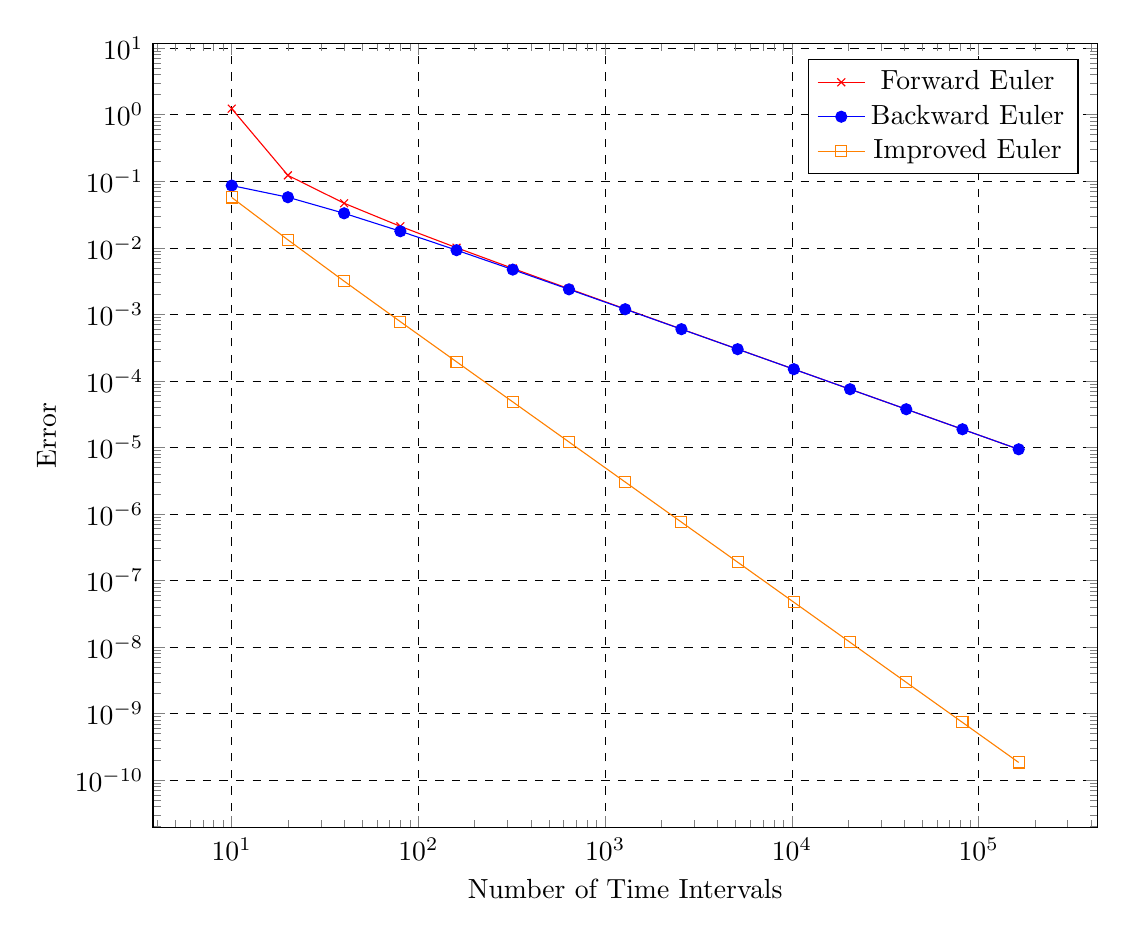
\begin{tikzpicture} \begin{loglogaxis}
[scale=1.75,
 grid=major, 
 major grid style={color=black,line width=0.2pt, dashed},
 xlabel=Number of Time Intervals,
 ylabel=Error
]

\addplot[color=red,mark=x] coordinates {
 ( 10 , 1.23247 )
 ( 20 , 0.122582 )
 ( 40 , 0.0466919 )
 ( 80 , 0.0210092 )
 ( 160 , 0.0100231 )
 ( 320 , 0.00490141 )
 ( 640 , 0.00242432 )
 ( 1280 , 0.0012057 )
 ( 2560 , 0.000601248 )
 ( 5120 , 0.000300226 )
 ( 10240 , 0.000150014 )
 ( 20480 , 7.49822e-05 )
 ( 40960 , 3.74849e-05 )
 ( 81920 , 1.87409e-05 )
 ( 163840 , 9.37007e-06 )
};
\addlegendentry{Forward Euler}
\addplot[color=blue,mark=*] coordinates {
 ( 10 , 0.0861097 )
 ( 20 , 0.0575183 )
 ( 40 , 0.0329666 )
 ( 80 , 0.0177217 )
 ( 160 , 0.00921006 )
 ( 320 , 0.00469871 )
 ( 640 , 0.00237367 )
 ( 1280 , 0.00119304 )
 ( 2560 , 0.000598084 )
 ( 5120 , 0.000299435 )
 ( 10240 , 0.000149816 )
 ( 20480 , 7.49328e-05 )
 ( 40960 , 3.74726e-05 )
 ( 81920 , 1.87378e-05 )
 ( 163840 , 9.3693e-06 )
};
\addlegendentry{Backward Euler}
\addplot[color=orange,mark=square] coordinates {
 ( 10 , 0.0570718 )
 ( 20 , 0.0131649 )
 ( 40 , 0.00314873 )
 ( 80 , 0.000776307 )
 ( 160 , 0.00019336 )
 ( 320 , 4.82947e-05 )
 ( 640 , 1.20708e-05 )
 ( 1280 , 3.01753e-06 )
 ( 2560 , 7.54371e-07 )
 ( 5120 , 1.88592e-07 )
 ( 10240 , 4.7148e-08 )
 ( 20480 , 1.1787e-08 )
 ( 40960 , 2.94675e-09 )
 ( 81920 , 7.36685e-10 )
 ( 163840 , 1.84173e-10 )
};
\addlegendentry{Improved Euler}
\end{loglogaxis}
\end{tikzpicture}
\caption{Comparison of error for iterative methods.}
 \label{Fig:ode_convergenceOfMethodsExample}
\end{center}
\end{figure}

The error for the three different methods is plotted in Fig.~\ref{Fig:ode_convergenceOfMethodsExample}. The forward and backward Euler methods eventually converge to the same line, meaning that so long as $\Delta t$ is small enough, they both have the same error. By inspecting the plot the slope is $-1$, which is the expected result since the error scales as $\Delta t$. For large $\Delta t$ the error of the forward Euler method is greater, which is a consequence of the instability of the explicit method where the error tends to compound. Once the threshold for stability is met, the two methods have the small error.

From the plot it is clear that the improved Euler method always outperforms both the forward and backward Euler methods. The slope of the line is $-2$, confirming that the error indeed scales of $( \Delta t )^2$. As an added bonus, like backward Euler, it does not exhibit any instability problems that forward Euler has.

These comparisons would not be complete without mentioning the computational time to generate these solutions. Much of this depends upon the specific problem, how well the solvers are implemented (many advanced solvers can take advantage of sparsity or other structures of the matrices), and if the compiler can make any optimizations. For a relatively simplistic implementation of these methods with this problem, for the same number of time steps, the backward Euler takes about twice as long to run compared to forward Euler, and improved Euler takes about three times longer to run than forward Euler. Results may vary depending on various factors, but the trend is typical. 

Using a fixed time step is not a fair comparison, because the end user would run as long as necessary to get the required accuracy. Suppose an accuracy of $\epsilon \approx 10^{-6}$ is desired. For backward and forward Euler this is about $1.5 \times 10^6$ time steps on this problem. For improved Euler, this only requires about 2000 time steps. The run time estimate to get the same level of accuracy has the improved Euler method running about \emph{200 times faster} than forward Euler, which is effectively instantaneous on a modern computer.


%%%%%%%%%%%%%%%%%%%%%%%%%%%%%%%%%%%%%%%%%%%%%%%%%%%%%%%%%%%%%%%%%%%%%%%%%%%%%%%%%%%%%%%%%%%%%%%%
\subsection{Application to Nonlinear ODEs}

The numerical techniques we discussed may be applied to non-linear systems of ordinary differential equations as well where the vector of functions $\mathbf{f}$ in
\begin{align}
  \mathbf{y}'(t) = \mathbf{f}( t, \mathbf{y}(t) ), \quad \mathbf{y}(0) = \mathbf{y}_0, \nonumber
\end{align}
is any function of $\mathbf{y}(t)$.

The forward Euler method is simple to adapt. We can apply the forward difference to the derivative to get
\begin{align}
  \mathbf{y}_{n+1} = \mathbf{y}_n + \Delta t \mathbf{f}( t_n, \mathbf{y}_n ).
\end{align}
Since $\mathbf{y}_n$ is known, $\mathbf{f}( t_n, \mathbf{y}_n )$ may be evaluated explicitly and we can advance the solution in time.

For the implicit schemes, the solution technique is more difficult. For backward Euler, we have
\begin{align}
  \mathbf{y}_{n+1} = \mathbf{y}_n + \Delta t \mathbf{f}( t_{n+1}, \mathbf{y}_{n+1} ) ;
\end{align}
and for improved Euler
\begin{align}
  \mathbf{y}_{n+1} = \mathbf{y}_n + \frac{\Delta t}{2} \left( \mathbf{f}( t_n, \mathbf{y}_n ) + \mathbf{f}( t_{n+1}, \mathbf{y}_{n+1} ) \right) .
\end{align}
The issue is that $\mathbf{f}( t_{n+1}, \mathbf{y}_{n+1} )$ depends upon $y_{n+1}$, which is unknown. If $\mathbf{f}( t, \mathbf{y} )$ is linear in $\mathbf{y}$, then we can solve a linear system as before. If it is not, then we need to use an interative numerical root finding algorithm such as the Newton-Raphson method.

Before discussing the Newton-Raphson method, it is worth commenting that the conclusions regarding convergence and stability assume a \emph{linear} system of equations. If this condition is not met, then there is little that can be said in general about the rate of convergence of particular algorithms, or even whether a particular algorithm will converge. Despite this, the general trends of convergence and stability tend to hold reasonably well and methods such as improved Euler tend to perform well in practice. 


%%%%%%%%%%%%%%%%%%%%%%%%%%%%%%%%%%%%%%%%%%%%%%%%%%%%%%%%%%%%%%%%%%%%%%%%%%%%%%%%%%%%%%%%%%%%%%%%
\subsection{Newton-Raphson Iteration}

Newton-Raphson is a classic iterative technique to find a root of a function
\begin{align}
  g(x) = 0. \nonumber
\end{align}
The idea is given a guess for the root, call it $x^{(k)}$, we use the first derivative to write an equation for a line about that point
\begin{align}
  y = g(x^{(k)}) + g'(x^{(k)}) ( x - x^{(k)} ).
\end{align}
If we set $y = 0$, we can use the equation for a line to solve for the unknown value $x$ that we set to the value for the next iteration or $x^{(k+1)}$:
\begin{align}
  x^{(k+1)} = x^{(k)} - \frac{ g(x^{(k)}) }{ g'(x^{(k)}) }.
\end{align}
This process may be repeated again and again, and, if the method converges, we will eventually find a good approximation for a root of $g(x)$. A key point here is \emph{if the method converges}. Being a nonlinear iteration, the Newton-Raphson is not guaranteed to converge. However, when it does, it tends to converge in a way that the error decreases geometrically fast. (If Newton's method fails, in practice, many applications switch over to a slower, but more robust, bisection method.)

The Newton-Raphson method may be generalized to find the roots of a vector of functions
\begin{align}
  \mathbf{g}(\mathbf{x}) = \mathbf{0} \nonumber
\end{align}
or in vector form
\begin{align}
  \left[ \begin{array}{c} g_1(x_1,x_2,\cdots,x_N) \\ g_2(x_1,x_2,\cdots,x_N) \\ \vdots \\ g_N(x_1,x_2,\cdots,x_N) \\ \end{array} \right] =
  \left[ \begin{array}{c} 0 \\ 0 \\ \vdots \\ 0 \end{array} \right] . \nonumber
\end{align}
In a similar fashion, we write a series of equations for lines and find where those lines converge to zero. The resulting iteration scheme has the following form:
\begin{align}
  \mathbf{x}^{(k+1)} = \mathbf{x}^{(k)} - \mathbf{J}^{-1}(\mathbf{x}^{(k)}) \mathbf{g}(\mathbf{x}^{(k)}) .
\end{align}
The matrix $\mathbf{J}(\mathbf{x})$ is called the \emph{Jacobian matrix} and is the multidimensional version of the first derivative:
\begin{align}
  \mathbf{J}(\mathbf{x}) = \left[ \begin{array}{c c c c}
  \dfrac{\partial g_1}{\partial x_1} & \dfrac{\partial g_1}{\partial x_2} & \cdots & \dfrac{\partial g_1}{\partial x_N} \\
  \dfrac{\partial g_2}{\partial x_1} & \dfrac{\partial g_2}{\partial x_2} & \cdots & \dfrac{\partial g_2}{\partial x_N} \\
  \vdots & \vdots & \ddots & \vdots \\
  \dfrac{\partial g_N}{\partial x_1} & \dfrac{\partial g_N}{\partial x_2} & \cdots & \dfrac{\partial g_N}{\partial x_N} \\ \end{array} \right] .
\end{align}
To avoid computing the inverse of the Jacobian matrix we often rewrite the Newton-Raphson iteration as a linear system
\begin{align}
  \mathbf{J}(\mathbf{x}^{(k)}) \mathbf{x}^{(k+1)} = \mathbf{J}(\mathbf{x}^{(k)}) \mathbf{x}^{(k)} -\mathbf{g}(\mathbf{x}^{(k)}) .
\end{align}
Since $\mathbf{x}^{(k)}$ is known, the right-hand side is completely known, and the solution vector $\mathbf{x}^{(k+1)}$ can be obtained by solving the linear system using techniques such as Gaussian elimination. 

The iteration begins with some initial guess $\mathbf{x}^{(0)}$ and continues until some user-defined convergence criterion is met, e.g.,
\begin{align}
  | \mathbf{x}^{(k+1)} - \mathbf{x}^{(k)} | < \epsilon.
\end{align}

Applied to backward Euler, the Newton-Raphson iteration is
\begin{align}
  \mathbf{g}(\mathbf{y}_{n+1}) = \mathbf{y}_{n+1} - \mathbf{y}_n - \Delta t \mathbf{f}( t_{n+1}, \mathbf{y}_{n+1} ) = \mathbf{0};
\end{align}
and for improved Euler,
\begin{align}
  \mathbf{g}(\mathbf{y}_{n+1}) = \mathbf{y}_{n+1} - \mathbf{y}_n - \frac{\Delta t}{2} \left( \mathbf{f}( t_n, \mathbf{y}_n ) + \mathbf{f}( t_{n+1}, \mathbf{y}_{n+1} ) \right) = \mathbf{0}.
\end{align}

A Newton-Raphson iteration must be performed each time step, similar to how a linear solve was done in the linear case. Note that each time step may require several Newton-Raphson iterations, for which each requires the solution of a linear system of equations. Usually the initial guess for the Newton-Raphson iteration is $\mathbf{y}_{n}$, the vector at the previous time step. A potential concern is the nonconvergence of the Newton-Raphson iteration. Fortunately, for sufficiently small time steps, Newton-Raphson does tend to converge to a solution and do as such in few iterations.

%%%%%%%%%%%%%%%%%%%%%%%%%%%%%%%%%%%%%%%%%%%%%%%%%%%%%%%%%%%%%%%%%%%%%%%%%%%%%%%%%%%%%%%%%%%%%%%%
\subsection{Example: Fission Reactor Kinetics}

An application of a nonlinear system of equations is analysis of nuclear reactor kinetics. The criticality of a nuclear reactor drives the time behavior of the neutron population in the reactor. If the reactor is critical $(k = 1)$, the power stays constant; if the reactor is subcritical $(k < 1)$ the reactor power tends to fall exponentially; and if the reactor is supercritical $(k > 1)$, the reactor power tends to rise exponentially. If the power reaches a certain level, there is sufficient energy release from nuclear fission to significantly increase the temperature of the reactor. As the temperature changes, so do the nuclear interaction properties, e.g., changes in density moving the nuclei further apart or enhanced thermal motion leading to Doppler broadening of the nuclear resonances in the cross sections, and the criticality of the system changes, which, in turn, leads to a change in the rate of power increase, affecting the temperature, and so on.

The primary method of energy production is from nuclear fission, which is directly proportional to the number of neutrons in the reactor. However, there is one added complication in that a small fraction (a few fractions of a percent) of the fission products (called delayed neutron precursors) undergo $\beta^-$ decay and subsequently emit a neutron (called a delayed neutron) through its de-excitation process, which must be considered in the neutron balance. The time scale for a fission neutron producing another fission neutron (microseconds in a light-water reactor) is a few orders of magnitude shorter than the time scale for the radioactive decay emission of delayed neutrons (milliseconds to minutes). This means they need to be treated as separate differential equations.

The equation for the fission rate density is
\begin{align}
  \frac{dp}{dt} = \left( \frac{ \rho(t,T) - \beta }{ \Lambda } \right) p(t) + \frac{\lambda}{\Lambda} \zeta(t) + q(t).
\end{align}
Here $p(t)$ is the fission rate density; $\rho(t,T)$ is the reactivity, which is related to the criticality of the system through
\begin{align}
  \rho(t,T) = \frac{ k(t,T) - 1 }{ k(t,T) }, 
\end{align}
and is also a function of temperature; $\beta$ is the effective fraction of neutrons that emerge from decay of fission products, $\Lambda$ is the effective lifetime of the neutron, $\lambda$ is some averaged decay constant for the delayed neutron precursors; $\zeta(t)$ is related to the density of delayed neutron precursors; and $q(t)$ is a source density of neutrons. The delayed neutron precursors have the balance equation
\begin{align}
  \frac{d\zeta}{dt} = \beta p(t) - \lambda \zeta(t).
\end{align}
For the reactivity we assume that it is constant with the addition of term that is linearly dependent upon temperature $T$:
\begin{align}
  \rho(t,T) = \rho_0 + \gamma ( T(t) - T_0 ),
\end{align}
here $\gamma$ is a temperature feedback coefficient. The temperature is proportional to the fission rate and can be described with the equation
\begin{align}
  D c_p \frac{dT}{dt} = \kappa p(t) - h ( T(t) - T_0 ),
\end{align}
here the temperature $T$ is defined to be $T_0$ at the ambient temperature, $D$ is the mass density (often $\rho$ but this was used for reactivity), $c_p$ is the specific heat of the material, $\kappa$ is some fission to energy conversion factor, and $h$ is a heat transfer or cooling coefficient. We have explicitly assumed $D$, $c_p$, and $h$ are not functions of temperature, which is a simplification we can justify if the temperature change is small. We are also neglecting the heat generation from fission products, which assumes the fission product inventory is small (not a good assumption in a power reactor). Also, for short time transients on the order of milliseconds, we often neglect losses from cooling, which has a timescale of minutes.

Once the reactivity is inserted into the rate equation for fission, we end up with a nonlinear ODE:
\begin{align}
  \frac{dp}{dt} = \alpha p(t) + \frac{ \gamma }{ \Lambda } T(t) p(t)  + \frac{\lambda}{\Lambda} \zeta(t) + q(t).
\end{align}
where
\begin{align}
  \alpha = \frac{ \rho_0 - \beta }{ \Lambda }. \nonumber
\end{align}
The system is nonlinear because it contains a product term, namely $T(t) p(t)$.

To summarize, the equations to be solved are:
\begin{subequations}
\begin{align}
  \frac{dp}{dt} &= \left( \alpha  + \frac{ \gamma }{ \Lambda } T(t) \right) p(t)  + \frac{\lambda}{\Lambda} \zeta(t) + q(t), \\
  \frac{d\zeta}{dt} &= \beta p(t) - \lambda \zeta(t), \\
  \frac{dT}{dt} &= \frac{\kappa}{D c_p } p(t) - \frac{h}{D c_p } T(t) .
\end{align}
\end{subequations}

Applying forward Euler to this system yields the system of algebraic equations
\begin{subequations}
\begin{align}
  p_{n+1}     &= \left( 1 + \alpha \Delta t + \frac{ \gamma \Delta t }{ \Lambda } T_n \right) p_n + \frac{\lambda \Delta t}{\Lambda} \zeta_n + \Delta t q_n, \\
  \zeta_{n+1} &= ( 1 - \lambda \Delta t ) \zeta_n + \beta p_n, \\
  T_{n+1}     &= \left( 1 - \frac{h \Delta t}{D c_p } \right) T_n + \frac{\kappa \Delta t}{D c_p } p_n .
\end{align}
\end{subequations}
Since everything on the right-hand side is known, we can solve for the fission rate, precursor population, and temperature at the next time step directly.

Applying backward Euler yields the system
\begin{subequations}
\begin{align}
  g_1 &= \left( 1 - \alpha \Delta t - \frac{ \gamma \Delta t }{ \Lambda } T_{n+1} \right) p_{n+1} - \frac{\lambda \Delta t}{\Lambda} \zeta_{n+1} - \Delta t q_{n+1} - p_n = 0, \\
  g_2 &= ( 1 + \lambda \Delta t ) \zeta_{n+1} - \beta \Delta_t p_{n+1} - \zeta_n = 0, \\
  g_3 &= \left( 1 + \frac{h \Delta t}{ D c_p } \right) T_{n+1} - \frac{\kappa \Delta t}{D c_p } p_{n+1} - T_n = 0.
\end{align}
\end{subequations}
This system of equations is in the form necessary for the Newton-Raphson iteration. Now, we must compute the terms of the Jacobian matrix:
\begin{subequations}
\begin{align}
  \frac{\partial g_1}{\partial p_{n+1}}     &= 1 - \alpha \Delta t - \frac{ \gamma \Delta t }{ \Lambda } T_{n+1}, \\
  \frac{\partial g_1}{\partial \zeta_{n+1}} &= - \frac{\lambda \Delta t}{\Lambda}, \\
  \frac{\partial g_1}{\partial T_{n+1}}     &= - \frac{ \gamma \Delta t }{ \Lambda } p_{n+1}, \\
  \frac{\partial g_2}{\partial p_{n+1}}     &= - \beta \Delta t, \\
  \frac{\partial g_2}{\partial \zeta_{n+1}} &= 1 + \lambda \Delta t , \\
  \frac{\partial g_2}{\partial T_{n+1}}     &= 0, \\
  \frac{\partial g_3}{\partial p_{n+1}}     &=  - \frac{\kappa \Delta t}{D c_p }, \\
  \frac{\partial g_3}{\partial \zeta_{n+1}} &= 0 , \\
  \frac{\partial g_3}{\partial T_{n+1}}     &= 1 + \frac{h \Delta t}{ D c_p } .  
\end{align}
\end{subequations}
This gives the Jacobian matrix
\begin{align}
  \mathbf{J}(\mathbf{x}^{(k)})  = \left[ \begin{array}{c c c}
   1 - \alpha \Delta t - \dfrac{ \gamma \Delta t }{ \Lambda } T_{n+1}^{(k)} & - \dfrac{\lambda \Delta t}{\Lambda} & - \dfrac{ \gamma \Delta t }{ \Lambda } p_{n+1}^{(k)} \vspace{0.2cm}  \\
   - \beta \Delta t & 1 + \lambda \Delta t  & 0 \vspace{0.2cm}  \\
    - \dfrac{\kappa \Delta t}{D c_p } & 0 & 1 + \dfrac{h \Delta t}{ D c_p }  \end{array} \right]
\end{align}
where 
\begin{align}
  \mathbf{x}^{(k)} = \left[ \begin{array}{c} p_{n+1}^{(k)} \vspace{0.2cm} \\ \zeta_{n+1}^{(k)} \vspace{0.2cm} \\ T_{n+1}^{(k)} \\ \end{array} \right] .
\end{align}
The Newton-Raphson iteration is now done by solving the linear system
\begin{align}
  \mathbf{J}(\mathbf{x}^{(k)}) \mathbf{x}^{(k+1)} = \mathbf{J}(\mathbf{x}^{(k)}) \mathbf{x}^{(k)} -\mathbf{g}(\mathbf{x}^{(k)}) . \nonumber
\end{align}
A logical initial guess is
\begin{align}
  \mathbf{x}^{(0)} = \left[ \begin{array}{c} p_{n} \\ \zeta_{n} \\ T_{n} \\ \end{array} \right] ,
\end{align}
which are the quantities at the previous time step. The Newton-Raphson iteration proceeds until some convergence criterion is met. In practice, sometimes a maximum number of iterations needs to be set, because the method can end up bouncing back and forth changing only a small amount each time to avoid the code locking. Generally speaking, if convergence fails, this means that a smaller time step should be taken. Once the iteration completes, the quantities $p, \zeta, T$ for the next step are known and the time stepping algorithm continues by doing another Newton-Raphson iteration until the end of the simulation.

The equations for improved Euler are more complicated. These are
\begin{subequations}
\begin{align}
  g_1 &= \left( 1 - \frac{\alpha \Delta t}{2} - \frac{ \gamma \Delta t }{ 2 \Lambda } T_{n+1} \right) p_{n+1} - \frac{\lambda \Delta t}{2 \Lambda} \zeta_{n+1} \nonumber \\
      &- \left( 1 + \frac{\alpha \Delta t}{2} + \frac{ \gamma \Delta t }{ 2 \Lambda } T_{n} \right) p_{n} - \frac{\lambda \Delta t}{2 \Lambda} \zeta_{n}  
       - \frac{\Delta t}{2} ( q_n + q_{n+1} ) = 0, \\
  g_2 &= \left( 1 + \frac{\lambda \Delta t}{2} \right) \zeta_{n+1} - \frac{\beta \Delta t}{2} p_{n+1} 
       - \left( 1 - \frac{\lambda \Delta t}{2} \right) \zeta_n - \frac{\beta \Delta t}{2} p_{n} = 0, \\
  g_3 &= \left( 1 + \frac{h \Delta t}{ 2 D c_p } \right) T_{n+1} - \frac{\kappa \Delta t}{2 D c_p } p_{n+1} 
       - \left( 1 - \frac{h \Delta t}{ 2 D c_p } \right) T_n - \frac{\kappa \Delta t}{2 D c_p } p_n = 0.
\end{align}
\end{subequations}
The Jacobian matrix is mostly unchanged except for an extra factor of $\rfrac{1}{2}$ on the time steps:
\begin{align}
  \mathbf{J}(\mathbf{x}^{(k)})  = \left[ \begin{array}{c c c}
   1 - \dfrac{\alpha \Delta t}{2} - \dfrac{ \gamma \Delta t }{ 2\Lambda } T_{n+1}^{(k)} & - \dfrac{\lambda \Delta t}{2\Lambda} & - \dfrac{ \gamma \Delta t }{ 2\Lambda } p_{n+1}^{(k)} \vspace{0.2cm} \\
   - \dfrac{\beta \Delta t}{2} & 1 + \dfrac{\lambda \Delta t}{2}  & 0 \vspace{0.2cm} \\
    - \dfrac{\kappa \Delta t}{2 D c_p } & 0 & 1 + \dfrac{h \Delta t}{ 2 D c_p }  \end{array} \right] .
\end{align}
Otherwise the iteration sequence is unchanged from backward Euler.

The improved Euler method is applied to solve this problem numerically. The following constant values are used:
\begin{align}
  \Lambda  &= 2.5 \times 10^{-6} \text{ s}, \nonumber \\
  \beta    &= 0.0076, \nonumber \\
  \rho_0   &= 5 \beta = 0.038, \nonumber \\
  \gamma   &= -1 \times 10^{-4} \text{ K$^{-1}$}, \nonumber \\
  \lambda  &= 0.25 \text{ s$^{-1}$}, \nonumber \\
  c_p      &= 4.18 \text{ J g$^{-1}$ K$^{-1}$},  \nonumber \\
  D        &= 1.0 \text{ g cm$^{-3}$}, \nonumber \\
  \kappa   &= 3.2 \times 10^{-11} \text{ J/fission}, \nonumber \\
  h        &= 4 \times 10^{-3} \text{ J cm$^{-3}$ K$^{-1}$ s$^{-1}$ }, \nonumber \\
  p(0)     &= 1000 \text{ fissions cm$^{-3}$ s$^{-1}$}, \nonumber \\
  \zeta(0) &= 0 \text{ precursors cm$^{-3}$}, \nonumber \\
  T(0)     &= T_0 \text{ K (note $T = T_0$ corresponds to ambient temperature)}, \nonumber \\
  q(t)     &= 0.01 \text{ neutrons cm$^{-3}$ s$^{-1}$ (constant)}. \nonumber
\end{align}
At time $t = 0$ a instantaneous insertion of reactivity $\rho_0 = 5\$$ is made. The fission rate density is plotted on log-log scale in Fig.~\ref{Fig:ode_fissionRateDensity} and the delayed neutron precursor density is plotted in log-log scale in Fig.~\ref{Fig:ode_precursorDensity}. The temperature and effective multiplication factor are plotted in Figs.~\ref{Fig:ode_temperatureChange} and~\ref{Fig:ode_effectiveMultiplication} respectively.

\begin{figure}[tb!]
\begin{center}
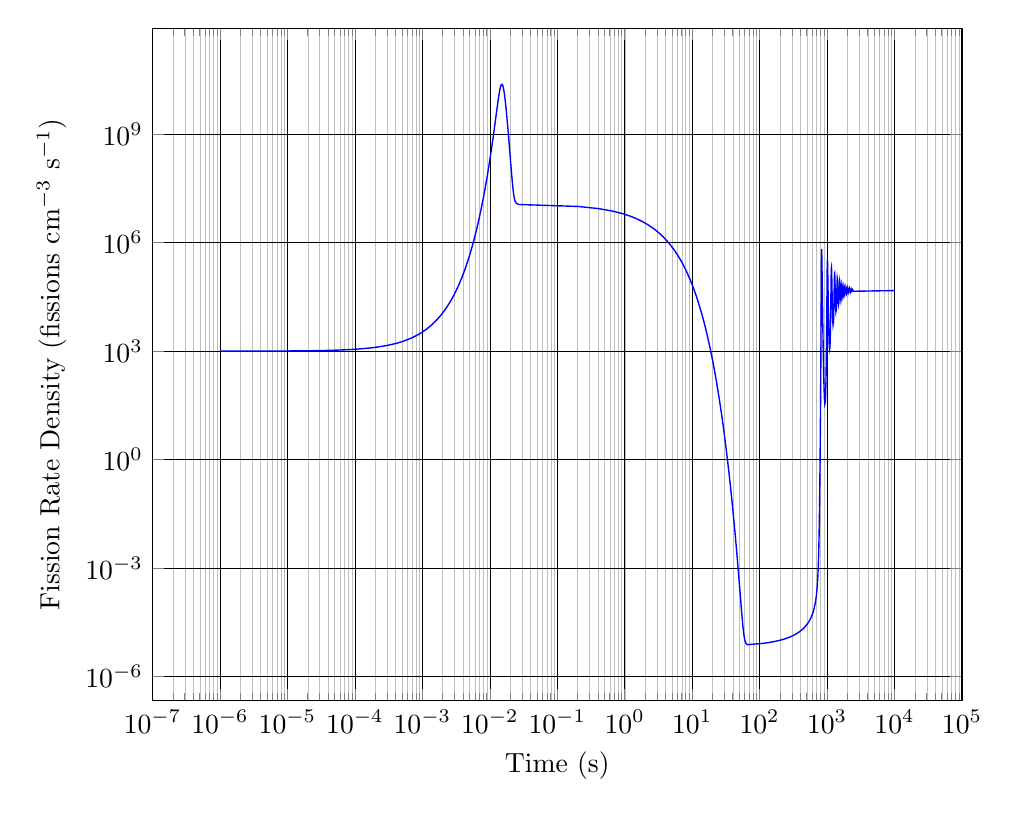
\begin{tikzpicture} \begin{loglogaxis}
[scale=1.5,
 grid=both, 
 major grid style={color=black,line width=0.2pt},
 minor grid style={color=gray!50,line width=0.1pt},
 xlabel=Time (s),
 ylabel=Fission Rate Density (fissions cm$^{-3}$ s$^{-1}$)
]

\addplot[color=blue, line width=0.5pt] coordinates {
 ( 1.0e-6, 1000 )
 ( 2.5e-06 , 1003.04 )
 ( 5e-06 , 1006.1 )
 ( 7.5e-06 , 1009.16 )
 ( 1e-05 , 1012.23 )
 ( 1.25e-05 , 1015.32 )
 ( 1.5e-05 , 1018.41 )
 ( 1.75e-05 , 1021.51 )
 ( 2e-05 , 1024.62 )
 ( 2.25e-05 , 1027.74 )
 ( 2.5e-05 , 1030.87 )
 ( 2.75e-05 , 1034.01 )
 ( 3.25e-05 , 1040.31 )
 ( 3.75e-05 , 1046.66 )
 ( 4.25e-05 , 1053.04 )
 ( 4.75e-05 , 1059.46 )
 ( 5.25e-05 , 1065.92 )
 ( 5.7705e-05 , 1072.69 )
 ( 6.34074e-05 , 1080.15 )
 ( 6.96508e-05 , 1088.39 )
 ( 7.64822e-05 , 1097.46 )
 ( 8.39516e-05 , 1107.48 )
 ( 9.21121e-05 , 1118.52 )
 ( 0.00010102 , 1130.71 )
 ( 0.000110736 , 1144.14 )
 ( 0.000121322 , 1158.97 )
 ( 0.000132845 , 1175.32 )
 ( 0.000145372 , 1193.36 )
 ( 0.000158974 , 1213.27 )
 ( 0.000173726 , 1235.23 )
 ( 0.000189702 , 1259.46 )
 ( 0.000206978 , 1286.2 )
 ( 0.00022563 , 1315.7 )
 ( 0.000245735 , 1348.27 )
 ( 0.000267368 , 1384.21 )
 ( 0.000290604 , 1423.88 )
 ( 0.000315511 , 1467.66 )
 ( 0.000342158 , 1516 )
 ( 0.000370606 , 1569.37 )
 ( 0.000400911 , 1628.28 )
 ( 0.000433125 , 1693.34 )
 ( 0.000467288 , 1765.17 )
 ( 0.000503434 , 1844.49 )
 ( 0.000541589 , 1932.1 )
 ( 0.000581768 , 2028.85 )
 ( 0.000623977 , 2135.71 )
 ( 0.000668212 , 2253.75 )
 ( 0.000714458 , 2384.14 )
 ( 0.000762693 , 2528.19 )
 ( 0.000812884 , 2687.32 )
 ( 0.000864989 , 2863.12 )
 ( 0.000918961 , 3057.36 )
 ( 0.000974741 , 3271.98 )
 ( 0.00103227 , 3509.11 )
 ( 0.00109148 , 3771.13 )
 ( 0.0011523 , 4060.67 )
 ( 0.00121465 , 4380.61 )
 ( 0.00127847 , 4734.15 )
 ( 0.00134367 , 5124.85 )
 ( 0.00141017 , 5556.6 )
 ( 0.0014779 , 6033.72 )
 ( 0.00154678 , 6561 )
 ( 0.00161674 , 7143.72 )
 ( 0.0016877 , 7787.69 )
 ( 0.00175959 , 8499.38 )
 ( 0.00183236 , 9285.91 )
 ( 0.00190592 , 10155.1 )
 ( 0.00198024 , 11115.8 )
 ( 0.00205523 , 12177.5 )
 ( 0.00213086 , 13350.8 )
 ( 0.00220707 , 14647.6 )
 ( 0.00228381 , 16080.8 )
 ( 0.00236104 , 17664.6 )
 ( 0.00243873 , 19415.2 )
 ( 0.00251682 , 21349.8 )
 ( 0.00259528 , 23487.9 )
 ( 0.00267409 , 25850.9 )
 ( 0.00275322 , 28462.6 )
 ( 0.00283262 , 31348.9 )
 ( 0.00291229 , 34538.8 )
 ( 0.00299219 , 38064.3 )
 ( 0.00307231 , 41960.7 )
 ( 0.00315263 , 46266.9 )
 ( 0.00323312 , 51026.1 )
 ( 0.00331378 , 56285.9 )
 ( 0.00339458 , 62099 )
 ( 0.00347551 , 68523.7 )
 ( 0.00355657 , 75624.1 )
 ( 0.00363774 , 83471.5 )
 ( 0.003719 , 92144.4 )
 ( 0.00380036 , 101730 )
 ( 0.0038818 , 112323 )
 ( 0.00396331 , 124031 )
 ( 0.00404489 , 136970 )
 ( 0.00412653 , 151271 )
 ( 0.00420823 , 167076 )
 ( 0.00428998 , 184544 )
 ( 0.00437177 , 203849 )
 ( 0.00445361 , 225184 )
 ( 0.00453548 , 248764 )
 ( 0.00461738 , 274825 )
 ( 0.00469932 , 303627 )
 ( 0.00478128 , 335459 )
 ( 0.00486327 , 370639 )
 ( 0.00494528 , 409520 )
 ( 0.00502731 , 452491 )
 ( 0.00510936 , 499982 )
 ( 0.00519143 , 552469 )
 ( 0.00527351 , 610478 )
 ( 0.00535561 , 674588 )
 ( 0.00543772 , 745442 )
 ( 0.00551984 , 823750 )
 ( 0.00560197 , 910295 )
 ( 0.00568411 , 1.00594e+06 )
 ( 0.00576626 , 1.11165e+06 )
 ( 0.00584841 , 1.22848e+06 )
 ( 0.00593057 , 1.3576e+06 )
 ( 0.00601274 , 1.5003e+06 )
 ( 0.00609492 , 1.65802e+06 )
 ( 0.0061771 , 1.83232e+06 )
 ( 0.00625928 , 2.02496e+06 )
 ( 0.00634147 , 2.23786e+06 )
 ( 0.00642367 , 2.47315e+06 )
 ( 0.00650586 , 2.7332e+06 )
 ( 0.00658806 , 3.02059e+06 )
 ( 0.00667027 , 3.33822e+06 )
 ( 0.00675247 , 3.68926e+06 )
 ( 0.00683468 , 4.07723e+06 )
 ( 0.00691689 , 4.506e+06 )
 ( 0.00699911 , 4.97987e+06 )
 ( 0.00708132 , 5.50358e+06 )
 ( 0.00716354 , 6.08238e+06 )
 ( 0.00724576 , 6.72206e+06 )
 ( 0.00732798 , 7.42901e+06 )
 ( 0.0074102 , 8.21032e+06 )
 ( 0.00749243 , 9.07381e+06 )
 ( 0.00757465 , 1.00281e+07 )
 ( 0.00765688 , 1.10828e+07 )
 ( 0.00773911 , 1.22484e+07 )
 ( 0.00782134 , 1.35365e+07 )
 ( 0.00790357 , 1.49601e+07 )
 ( 0.00798581 , 1.65335e+07 )
 ( 0.00806805 , 1.82722e+07 )
 ( 0.00815028 , 2.01938e+07 )
 ( 0.00823252 , 2.23175e+07 )
 ( 0.00831477 , 2.46645e+07 )
 ( 0.00839701 , 2.72581e+07 )
 ( 0.00847926 , 3.01245e+07 )
 ( 0.00856151 , 3.32922e+07 )
 ( 0.00864377 , 3.67928e+07 )
 ( 0.00872602 , 4.06615e+07 )
 ( 0.00880828 , 4.49366e+07 )
 ( 0.00889055 , 4.96611e+07 )
 ( 0.00897282 , 5.4882e+07 )
 ( 0.00905509 , 6.06514e+07 )
 ( 0.00913737 , 6.70269e+07 )
 ( 0.00921965 , 7.4072e+07 )
 ( 0.00930195 , 8.18571e+07 )
 ( 0.00938424 , 9.04595e+07 )
 ( 0.00946655 , 9.99651e+07 )
 ( 0.00954886 , 1.10468e+08 )
 ( 0.00963119 , 1.22074e+08 )
 ( 0.00971352 , 1.34896e+08 )
 ( 0.00979586 , 1.49064e+08 )
 ( 0.00987822 , 1.64717e+08 )
 ( 0.00996059 , 1.82011e+08 )
 ( 0.010043 , 2.01116e+08 )
 ( 0.0101254 , 2.22222e+08 )
 ( 0.0102078 , 2.45536e+08 )
 ( 0.0102902 , 2.7129e+08 )
 ( 0.0103727 , 2.99737e+08 )
 ( 0.0104552 , 3.31155e+08 )
 ( 0.0105377 , 3.65854e+08 )
 ( 0.0106203 , 4.04173e+08 )
 ( 0.0107029 , 4.46486e+08 )
 ( 0.0107855 , 4.93204e+08 )
 ( 0.0108681 , 5.44783e+08 )
 ( 0.0109508 , 6.01719e+08 )
 ( 0.0110336 , 6.64563e+08 )
 ( 0.0111164 , 7.33917e+08 )
 ( 0.0111993 , 8.10444e+08 )
 ( 0.0112823 , 8.94872e+08 )
 ( 0.0113653 , 9.87998e+08 )
 ( 0.0114484 , 1.0907e+09 )
 ( 0.0115316 , 1.20393e+09 )
 ( 0.0116149 , 1.32873e+09 )
 ( 0.0116983 , 1.46626e+09 )
 ( 0.0117819 , 1.61776e+09 )
 ( 0.0118656 , 1.78459e+09 )
 ( 0.0119494 , 1.96823e+09 )
 ( 0.0120334 , 2.17028e+09 )
 ( 0.0121177 , 2.39249e+09 )
 ( 0.0122021 , 2.63671e+09 )
 ( 0.0122868 , 2.90498e+09 )
 ( 0.0123717 , 3.19946e+09 )
 ( 0.0124569 , 3.52247e+09 )
 ( 0.0125425 , 3.87645e+09 )
 ( 0.0126284 , 4.264e+09 )
 ( 0.0127147 , 4.68786e+09 )
 ( 0.0128015 , 5.15085e+09 )
 ( 0.0128888 , 5.65589e+09 )
 ( 0.0129767 , 6.20592e+09 )
 ( 0.0130652 , 6.8039e+09 )
 ( 0.0131544 , 7.45269e+09 )
 ( 0.0132444 , 8.15495e+09 )
 ( 0.0133354 , 8.91308e+09 )
 ( 0.0134273 , 9.72899e+09 )
 ( 0.0135204 , 1.06039e+10 )
 ( 0.0136148 , 1.15382e+10 )
 ( 0.0137107 , 1.2531e+10 )
 ( 0.0138083 , 1.35797e+10 )
 ( 0.0139079 , 1.46795e+10 )
 ( 0.0140096 , 1.58231e+10 )
 ( 0.014114 , 1.69993e+10 )
 ( 0.0142214 , 1.81926e+10 )
 ( 0.0143324 , 1.93818e+10 )
 ( 0.0144475 , 2.05386e+10 )
 ( 0.0145676 , 2.16259e+10 )
 ( 0.0146938 , 2.2596e+10 )
 ( 0.0148273 , 2.33879e+10 )
 ( 0.0149701 , 2.39248e+10 )
 ( 0.0151246 , 2.4111e+10 )
 ( 0.0152944 , 2.38292e+10 )
 ( 0.015485 , 2.29378e+10 )
 ( 0.0157049 , 2.12705e+10 )
 ( 0.0159259 , 1.91035e+10 )
 ( 0.0161754 , 1.63512e+10 )
 ( 0.0163828 , 1.40274e+10 )
 ( 0.0165675 , 1.20464e+10 )
 ( 0.0167379 , 1.03514e+10 )
 ( 0.0168984 , 8.89829e+09 )
 ( 0.0170516 , 7.65123e+09 )
 ( 0.0171994 , 6.58022e+09 )
 ( 0.0173429 , 5.65997e+09 )
 ( 0.017483 , 4.86896e+09 )
 ( 0.0176205 , 4.18888e+09 )
 ( 0.0177558 , 3.60405e+09 )
 ( 0.0178893 , 3.10106e+09 )
 ( 0.0180214 , 2.6684e+09 )
 ( 0.0181522 , 2.29619e+09 )
 ( 0.0182821 , 1.97598e+09 )
 ( 0.0184113 , 1.70047e+09 )
 ( 0.0185397 , 1.46341e+09 )
 ( 0.0186677 , 1.25943e+09 )
 ( 0.0187953 , 1.08391e+09 )
 ( 0.0189227 , 9.32861e+08 )
 ( 0.0190499 , 8.0288e+08 )
 ( 0.019177 , 6.91022e+08 )
 ( 0.0193041 , 5.94759e+08 )
 ( 0.0194313 , 5.11915e+08 )
 ( 0.0195588 , 4.40618e+08 )
 ( 0.0196865 , 3.79259e+08 )
 ( 0.0198147 , 3.26452e+08 )
 ( 0.0199434 , 2.81005e+08 )
 ( 0.0200728 , 2.41891e+08 )
 ( 0.020203 , 2.08228e+08 )
 ( 0.0203343 , 1.79256e+08 )
 ( 0.0204667 , 1.54322e+08 )
 ( 0.0206007 , 1.32862e+08 )
 ( 0.0207364 , 1.14393e+08 )
 ( 0.0208743 , 9.84984e+07 )
 ( 0.0210148 , 8.4819e+07 )
 ( 0.0211585 , 7.30466e+07 )
 ( 0.021306 , 6.29155e+07 )
 ( 0.0214584 , 5.41975e+07 )
 ( 0.0216167 , 4.66959e+07 )
 ( 0.0217825 , 4.02418e+07 )
 ( 0.021958 , 3.46898e+07 )
 ( 0.0221463 , 2.99152e+07 )
 ( 0.0223519 , 2.58109e+07 )
 ( 0.0225819 , 2.22857e+07 )
 ( 0.0228484 , 1.92624e+07 )
 ( 0.0231746 , 1.66773e+07 )
 ( 0.0236127 , 1.44835e+07 )
 ( 0.0243294 , 1.2667e+07 )
 ( 0.0267446 , 1.13946e+07 )
 ( 0.202966 , 1.00615e+07 )
 ( 0.410704 , 8.76663e+06 )
 ( 0.674763 , 7.42503e+06 )
 ( 0.953514 , 6.28143e+06 )
 ( 1.23378 , 5.34251e+06 )
 ( 1.5155 , 4.56225e+06 )
 ( 1.79858 , 3.90801e+06 )
 ( 2.08293 , 3.3557e+06 )
 ( 2.36843 , 2.88698e+06 )
 ( 2.65497 , 2.48755e+06 )
 ( 2.94247 , 2.14606e+06 )
 ( 3.23083 , 1.85333e+06 )
 ( 3.51998 , 1.60186e+06 )
 ( 3.80984 , 1.38546e+06 )
 ( 4.10034 , 1.19897e+06 )
 ( 4.39142 , 1.03807e+06 )
 ( 4.68303 , 899111 )
 ( 4.97513 , 779002 )
 ( 5.26766 , 675117 )
 ( 5.5606 , 585214 )
 ( 5.8539 , 507374 )
 ( 6.14754 , 439953 )
 ( 6.44149 , 381537 )
 ( 6.73572 , 330910 )
 ( 7.03022 , 287023 )
 ( 7.32496 , 248972 )
 ( 7.61993 , 215976 )
 ( 7.91511 , 187360 )
 ( 8.21048 , 162540 )
 ( 8.50603 , 141011 )
 ( 8.80176 , 122334 )
 ( 9.09765 , 106132 )
 ( 9.39369 , 92076.5 )
 ( 9.68987 , 79881.8 )
 ( 9.98619 , 69301.9 )
 ( 10.2826 , 60122.7 )
 ( 10.5792 , 52158.7 )
 ( 10.8759 , 45249.1 )
 ( 11.1727 , 39254.2 )
 ( 11.4696 , 34053.1 )
 ( 11.7666 , 29540.6 )
 ( 12.0638 , 25625.7 )
 ( 12.361 , 22229.2 )
 ( 12.6583 , 19282.5 )
 ( 12.9557 , 16726.1 )
 ( 13.2532 , 14508.3 )
 ( 13.5508 , 12584.4 )
 ( 13.8484 , 10915.4 )
 ( 14.1462 , 9467.56 )
 ( 14.444 , 8211.6 )
 ( 14.7419 , 7122.12 )
 ( 15.0399 , 6177.07 )
 ( 15.338 , 5357.32 )
 ( 15.6361 , 4646.26 )
 ( 15.9343 , 4029.51 )
 ( 16.2326 , 3494.56 )
 ( 16.531 , 3030.57 )
 ( 16.8294 , 2628.13 )
 ( 17.1279 , 2279.1 )
 ( 17.4265 , 1976.38 )
 ( 17.7251 , 1713.84 )
 ( 18.0238 , 1486.15 )
 ( 18.3226 , 1288.68 )
 ( 18.6215 , 1117.44 )
 ( 18.9204 , 968.928 )
 ( 19.2194 , 840.141 )
 ( 19.5185 , 728.459 )
 ( 19.8176 , 631.612 )
 ( 20.1168 , 547.631 )
 ( 20.4161 , 474.809 )
 ( 20.7154 , 411.663 )
 ( 21.0148 , 356.908 )
 ( 21.3143 , 309.432 )
 ( 21.6138 , 268.266 )
 ( 21.9134 , 232.572 )
 ( 22.2131 , 201.625 )
 ( 22.5128 , 174.792 )
 ( 22.8126 , 151.528 )
 ( 23.1125 , 131.358 )
 ( 23.4124 , 113.871 )
 ( 23.7124 , 98.7104 )
 ( 24.0125 , 85.5667 )
 ( 24.3126 , 74.172 )
 ( 24.6128 , 64.2936 )
 ( 24.9131 , 55.73 )
 ( 25.2134 , 48.3062 )
 ( 25.5138 , 41.8706 )
 ( 25.8142 , 36.2919 )
 ( 26.1148 , 31.4559 )
 ( 26.4153 , 27.264 )
 ( 26.716 , 23.6303 )
 ( 27.0167 , 20.4806 )
 ( 27.3175 , 17.7504 )
 ( 27.6183 , 15.384 )
 ( 27.9192 , 13.3328 )
 ( 28.2201 , 11.555 )
 ( 28.5212 , 10.0141 )
 ( 28.8222 , 8.67858 )
 ( 29.1234 , 7.52107 )
 ( 29.4246 , 6.51786 )
 ( 29.7258 , 5.64841 )
 ( 30.0271 , 4.89488 )
 ( 30.3284 , 4.24184 )
 ( 30.6298 , 3.6759 )
 ( 30.9313 , 3.18544 )
 ( 31.2328 , 2.7604 )
 ( 31.5343 , 2.39207 )
 ( 31.8359 , 2.07289 )
 ( 32.1374 , 1.79629 )
 ( 32.4391 , 1.55661 )
 ( 32.7407 , 1.34892 )
 ( 33.0423 , 1.16895 )
 ( 33.344 , 1.01301 )
 ( 33.6456 , 0.877884 )
 ( 33.9472 , 0.760803 )
 ( 34.2488 , 0.659357 )
 ( 34.5504 , 0.57146 )
 ( 34.8518 , 0.495303 )
 ( 35.1532 , 0.429319 )
 ( 35.4545 , 0.37215 )
 ( 35.7557 , 0.32262 )
 ( 36.0566 , 0.279708 )
 ( 36.3574 , 0.24253 )
 ( 36.658 , 0.210321 )
 ( 36.9582 , 0.182417 )
 ( 37.2581 , 0.158243 )
 ( 37.5577 , 0.1373 )
 ( 37.8567 , 0.119156 )
 ( 38.1553 , 0.103438 )
 ( 38.4532 , 0.0898211 )
 ( 38.7504 , 0.078024 )
 ( 39.0468 , 0.0678034 )
 ( 39.3423 , 0.0589484 )
 ( 39.6368 , 0.051276 )
 ( 39.93 , 0.044628 )
 ( 40.2219 , 0.038867 )
 ( 40.5124 , 0.0338741 )
 ( 40.8012 , 0.0295461 )
 ( 41.0882 , 0.0257937 )
 ( 41.3731 , 0.0225395 )
 ( 41.6424 , 0.0198435 )
 ( 41.8814 , 0.0177217 )
 ( 42.1303 , 0.0157465 )
 ( 42.3834 , 0.0139758 )
 ( 42.6394 , 0.0123825 )
 ( 42.872 , 0.0110928 )
 ( 43.1174 , 0.00987602 )
 ( 43.3491 , 0.00885274 )
 ( 43.5901 , 0.00789997 )
 ( 43.8124 , 0.00711225 )
 ( 44.0431 , 0.00637807 )
 ( 44.2788 , 0.00570619 )
 ( 44.5162 , 0.00510123 )
 ( 44.7528 , 0.00456232 )
 ( 44.9866 , 0.00408566 )
 ( 45.2164 , 0.00366603 )
 ( 45.441 , 0.00329756 )
 ( 45.6729 , 0.00295609 )
 ( 45.8963 , 0.00266066 )
 ( 46.1222 , 0.00239204 )
 ( 46.3481 , 0.00215074 )
 ( 46.5718 , 0.00193575 )
 ( 46.8001 , 0.00173861 )
 ( 47.0297 , 0.00156069 )
 ( 47.2581 , 0.00140183 )
 ( 47.4836 , 0.00126098 )
 ( 47.7102 , 0.00113376 )
 ( 47.9356 , 0.00102004 )
 ( 48.1624 , 0.000917192 )
 ( 48.3882 , 0.000825188 )
 ( 48.6112 , 0.000743472 )
 ( 48.8366 , 0.00066917 )
 ( 49.0618 , 0.000602449 )
 ( 49.2873 , 0.000542357 )
 ( 49.5111 , 0.000488737 )
 ( 49.7359 , 0.000440287 )
 ( 49.9594 , 0.00039695 )
 ( 50.1835 , 0.000357856 )
 ( 50.4076 , 0.000322682 )
 ( 50.6313 , 0.000291109 )
 ( 50.8551 , 0.000262669 )
 ( 51.0796 , 0.000237018 )
 ( 51.3046 , 0.000213888 )
 ( 51.5291 , 0.000193137 )
 ( 51.7539 , 0.00017445 )
 ( 51.9785 , 0.000157654 )
 ( 52.204 , 0.000142492 )
 ( 52.4295 , 0.000128858 )
 ( 52.655 , 0.000116604 )
 ( 52.8807 , 0.000105574 )
 ( 53.1068 , 9.56461e-05 )
 ( 53.3334 , 8.66977e-05 )
 ( 53.5604 , 7.86456e-05 )
 ( 53.7878 , 7.14005e-05 )
 ( 54.0157 , 6.48766e-05 )
 ( 54.2443 , 5.9003e-05 )
 ( 54.4734 , 5.3718e-05 )
 ( 54.7031 , 4.89621e-05 )
 ( 54.9336 , 4.468e-05 )
 ( 55.165 , 4.08248e-05 )
 ( 55.3975 , 3.73533e-05 )
 ( 55.6311 , 3.42282e-05 )
 ( 55.8658 , 3.14163e-05 )
 ( 56.1021 , 2.88838e-05 )
 ( 56.3399 , 2.66045e-05 )
 ( 56.5794 , 2.45528e-05 )
 ( 56.8209 , 2.27064e-05 )
 ( 57.0647 , 2.10441e-05 )
 ( 57.3111 , 1.95477e-05 )
 ( 57.5603 , 1.82006e-05 )
 ( 57.813 , 1.69881e-05 )
 ( 58.0693 , 1.58969e-05 )
 ( 58.33 , 1.49149e-05 )
 ( 58.5958 , 1.40309e-05 )
 ( 58.8673 , 1.32355e-05 )
 ( 59.1455 , 1.25198e-05 )
 ( 59.4317 , 1.18757e-05 )
 ( 59.7271 , 1.12963e-05 )
 ( 60.0337 , 1.0775e-05 )
 ( 60.3536 , 1.03063e-05 )
 ( 60.6898 , 9.88471e-06 )
 ( 61.0462 , 9.50574e-06 )
 ( 61.4281 , 9.16522e-06 )
 ( 61.8431 , 8.85945e-06 )
 ( 62.3022 , 8.58512e-06 )
 ( 62.8232 , 8.33935e-06 )
 ( 63.4364 , 8.11975e-06 )
 ( 64.2006 , 7.92452e-06 )
 ( 65.2575 , 7.75315e-06 )
 ( 67.1495 , 7.61032e-06 )
 ( 119.948 , 8.37135e-06 )
 ( 162.656 , 9.20848e-06 )
 ( 203.061 , 1.01293e-05 )
 ( 241.207 , 1.11423e-05 )
 ( 277.142 , 1.22565e-05 )
 ( 310.926 , 1.34821e-05 )
 ( 342.624 , 1.48304e-05 )
 ( 372.309 , 1.63134e-05 )
 ( 400.057 , 1.79447e-05 )
 ( 425.951 , 1.97392e-05 )
 ( 450.074 , 2.17131e-05 )
 ( 472.512 , 2.38845e-05 )
 ( 493.353 , 2.62729e-05 )
 ( 512.686 , 2.89002e-05 )
 ( 530.597 , 3.17903e-05 )
 ( 547.172 , 3.49693e-05 )
 ( 562.497 , 3.84662e-05 )
 ( 576.653 , 4.23129e-05 )
 ( 589.72 , 4.65442e-05 )
 ( 601.775 , 5.11987e-05 )
 ( 612.891 , 5.63185e-05 )
 ( 623.138 , 6.19504e-05 )
 ( 632.582 , 6.81456e-05 )
 ( 641.287 , 7.49604e-05 )
 ( 649.31 , 8.24565e-05 )
 ( 656.708 , 9.07023e-05 )
 ( 663.533 , 9.97726e-05 )
 ( 669.833 , 0.00010975 )
 ( 675.653 , 0.000120726 )
 ( 681.033 , 0.0001328 )
 ( 686.014 , 0.00014608 )
 ( 690.629 , 0.000160689 )
 ( 694.913 , 0.000176759 )
 ( 698.893 , 0.000194435 )
 ( 702.598 , 0.000213881 )
 ( 706.051 , 0.00023527 )
 ( 709.277 , 0.000258803 )
 ( 712.295 , 0.000284696 )
 ( 715.123 , 0.000313174 )
 ( 717.777 , 0.000344494 )
 ( 720.275 , 0.000378958 )
 ( 722.63 , 0.000416884 )
 ( 724.854 , 0.000458613 )
 ( 726.956 , 0.000504505 )
 ( 728.949 , 0.000555013 )
 ( 730.839 , 0.000610522 )
 ( 732.636 , 0.000671594 )
 ( 734.35 , 0.000738831 )
 ( 735.983 , 0.00081273 )
 ( 737.546 , 0.000894118 )
 ( 739.04 , 0.000983568 )
 ( 740.472 , 0.00108198 )
 ( 741.849 , 0.00119043 )
 ( 743.171 , 0.00130957 )
 ( 744.446 , 0.00144103 )
 ( 745.677 , 0.00158578 )
 ( 746.864 , 0.00174516 )
 ( 748.006 , 0.0019197 )
 ( 749.111 , 0.00211186 )
 ( 750.184 , 0.00232366 )
 ( 751.23 , 0.00255839 )
 ( 752.248 , 0.0028177 )
 ( 753.236 , 0.00310326 )
 ( 754.194 , 0.00341697 )
 ( 755.123 , 0.00376135 )
 ( 756.028 , 0.00414038 )
 ( 756.916 , 0.00456083 )
 ( 757.773 , 0.00501943 )
 ( 758.612 , 0.00552531 )
 ( 759.45 , 0.0060963 )
 ( 760.244 , 0.00670604 )
 ( 761.052 , 0.00740492 )
 ( 761.824 , 0.00815898 )
 ( 762.591 , 0.00900277 )
 ( 763.343 , 0.0099351 )
 ( 764.066 , 0.0109437 )
 ( 764.813 , 0.0121175 )
 ( 765.503 , 0.0133386 )
 ( 766.196 , 0.0147165 )
 ( 766.886 , 0.016259 )
 ( 767.563 , 0.0179603 )
 ( 768.21 , 0.019787 )
 ( 768.966 , 0.0222048 )
 ( 769.688 , 0.0248438 )
 ( 770.336 , 0.0275292 )
 ( 771.136 , 0.0313198 )
 ( 771.769 , 0.0347523 )
 ( 772.392 , 0.0385592 )
 ( 773.004 , 0.0427812 )
 ( 773.608 , 0.0474635 )
 ( 774.202 , 0.0526558 )
 ( 774.787 , 0.0584138 )
 ( 775.364 , 0.0647987 )
 ( 775.932 , 0.0718787 )
 ( 776.493 , 0.0797291 )
 ( 777.046 , 0.0884335 )
 ( 777.591 , 0.0980846 )
 ( 778.13 , 0.108785 )
 ( 778.661 , 0.120648 )
 ( 779.186 , 0.133801 )
 ( 779.704 , 0.148382 )
 ( 780.216 , 0.164547 )
 ( 780.721 , 0.182468 )
 ( 781.221 , 0.202333 )
 ( 781.715 , 0.224354 )
 ( 782.203 , 0.248765 )
 ( 782.686 , 0.275824 )
 ( 783.163 , 0.305817 )
 ( 783.635 , 0.339063 )
 ( 784.103 , 0.375912 )
 ( 784.565 , 0.416755 )
 ( 785.022 , 0.462023 )
 ( 785.475 , 0.512196 )
 ( 785.924 , 0.567803 )
 ( 786.367 , 0.629433 )
 ( 786.807 , 0.697734 )
 ( 787.242 , 0.77343 )
 ( 787.673 , 0.857318 )
 ( 788.1 , 0.950285 )
 ( 788.523 , 1.05331 )
 ( 788.943 , 1.16748 )
 ( 789.358 , 1.294 )
 ( 789.77 , 1.43419 )
 ( 790.178 , 1.58955 )
 ( 790.583 , 1.76152 )
 ( 790.982 , 1.95156 )
 ( 791.378 , 2.16159 )
 ( 791.77 , 2.39371 )
 ( 792.157 , 2.65025 )
 ( 792.541 , 2.93379 )
 ( 792.922 , 3.24718 )
 ( 793.299 , 3.59355 )
 ( 793.672 , 3.97638 )
 ( 794.043 , 4.39953 )
 ( 794.41 , 4.86724 )
 ( 794.775 , 5.3842 )
 ( 795.136 , 5.9556 )
 ( 795.495 , 6.58719 )
 ( 795.85 , 7.2853 )
 ( 796.203 , 8.05694 )
 ( 796.554 , 8.90987 )
 ( 796.902 , 9.85264 )
 ( 797.247 , 10.8947 )
 ( 797.59 , 12.0466 )
 ( 797.93 , 13.3198 )
 ( 798.269 , 14.7271 )
 ( 798.604 , 16.2827 )
 ( 798.938 , 18.0021 )
 ( 799.269 , 19.9027 )
 ( 799.598 , 22.0036 )
 ( 799.925 , 24.3257 )
 ( 800.25 , 26.8925 )
 ( 800.573 , 29.7296 )
 ( 800.893 , 32.8657 )
 ( 801.212 , 36.3321 )
 ( 801.529 , 40.1637 )
 ( 801.844 , 44.399 )
 ( 802.157 , 49.0804 )
 ( 802.468 , 54.255 )
 ( 802.777 , 59.9747 )
 ( 803.084 , 66.2969 )
 ( 803.39 , 73.2851 )
 ( 803.693 , 81.0095 )
 ( 803.995 , 89.5475 )
 ( 804.296 , 98.985 )
 ( 804.594 , 109.417 )
 ( 804.891 , 120.947 )
 ( 805.186 , 133.692 )
 ( 805.48 , 147.78 )
 ( 805.772 , 163.351 )
 ( 806.063 , 180.563 )
 ( 806.351 , 199.587 )
 ( 806.639 , 220.616 )
 ( 806.925 , 243.86 )
 ( 807.209 , 269.551 )
 ( 807.492 , 297.949 )
 ( 807.773 , 329.339 )
 ( 808.053 , 364.034 )
 ( 808.332 , 402.383 )
 ( 808.609 , 444.772 )
 ( 808.884 , 491.625 )
 ( 809.159 , 543.414 )
 ( 809.432 , 600.656 )
 ( 809.703 , 663.928 )
 ( 809.973 , 733.863 )
 ( 810.242 , 811.163 )
 ( 810.51 , 896.605 )
 ( 810.777 , 991.045 )
 ( 811.042 , 1095.43 )
 ( 811.306 , 1210.81 )
 ( 811.569 , 1338.34 )
 ( 811.83 , 1479.3 )
 ( 812.09 , 1635.11 )
 ( 812.35 , 1807.32 )
 ( 812.608 , 1997.66 )
 ( 812.865 , 2208.05 )
 ( 813.121 , 2440.6 )
 ( 813.375 , 2697.63 )
 ( 813.629 , 2981.72 )
 ( 813.882 , 3295.73 )
 ( 814.133 , 3642.8 )
 ( 814.384 , 4026.41 )
 ( 814.633 , 4450.41 )
 ( 814.882 , 4919.04 )
 ( 815.13 , 5437.01 )
 ( 815.377 , 6009.51 )
 ( 815.623 , 6642.27 )
 ( 815.868 , 7341.64 )
 ( 816.112 , 8114.62 )
 ( 816.356 , 8968.96 )
 ( 816.598 , 9913.2 )
 ( 816.84 , 10956.8 )
 ( 817.082 , 12110.2 )
 ( 817.322 , 13385 )
 ( 817.562 , 14793.9 )
 ( 817.802 , 16351.1 )
 ( 818.041 , 18072 )
 ( 818.28 , 19973.8 )
 ( 818.518 , 22075.7 )
 ( 818.756 , 24398.6 )
 ( 818.994 , 26965.7 )
 ( 819.231 , 29802.5 )
 ( 819.469 , 32937.5 )
 ( 819.706 , 36401.8 )
 ( 819.944 , 40230 )
 ( 820.182 , 44460.1 )
 ( 820.42 , 49130.1 )
 ( 820.659 , 54279 )
 ( 820.897 , 59953.3 )
 ( 821.136 , 66203.5 )
 ( 821.376 , 73084.2 )
 ( 821.616 , 80654.4 )
 ( 821.857 , 88977.4 )
 ( 822.099 , 98121.2 )
 ( 822.342 , 108158 )
 ( 822.587 , 119165 )
 ( 822.833 , 131222 )
 ( 823.082 , 144415 )
 ( 823.333 , 158832 )
 ( 823.588 , 174563 )
 ( 823.845 , 191698 )
 ( 824.107 , 210328 )
 ( 824.373 , 230540 )
 ( 824.645 , 252416 )
 ( 824.923 , 276026 )
 ( 825.209 , 301427 )
 ( 825.504 , 328651 )
 ( 825.81 , 357701 )
 ( 826.129 , 388537 )
 ( 826.463 , 421059 )
 ( 826.817 , 455082 )
 ( 827.195 , 490305 )
 ( 827.604 , 526256 )
 ( 828.056 , 562196 )
 ( 828.566 , 596947 )
 ( 829.514 , 641971 )
 ( 831.003 , 659292 )
 ( 833.734 , 569255 )
 ( 835.288 , 486829 )
 ( 836.564 , 417775 )
 ( 837.717 , 358917 )
 ( 838.799 , 308557 )
 ( 839.836 , 265340 )
 ( 840.842 , 228245 )
 ( 841.826 , 196354 )
 ( 842.794 , 168951 )
 ( 843.751 , 145375 )
 ( 844.7 , 125108 )
 ( 845.645 , 107663 )
 ( 846.585 , 92663.3 )
 ( 847.526 , 79748.8 )
 ( 848.465 , 68643.5 )
 ( 849.407 , 59079.8 )
 ( 850.35 , 50855.7 )
 ( 851.295 , 43782.9 )
 ( 852.242 , 37711.7 )
 ( 853.191 , 32496.1 )
 ( 854.142 , 28012 )
 ( 855.098 , 24154.4 )
 ( 856.059 , 20833.8 )
 ( 857.024 , 17974.3 )
 ( 857.997 , 15510.7 )
 ( 858.975 , 13387.5 )
 ( 859.962 , 11557 )
 ( 860.956 , 9978.45 )
 ( 861.959 , 8616.83 )
 ( 862.97 , 7442.11 )
 ( 863.992 , 6428.37 )
 ( 865.024 , 5553.46 )
 ( 866.067 , 4798.18 )
 ( 867.121 , 4146.12 )
 ( 868.188 , 3583.07 )
 ( 869.267 , 3096.85 )
 ( 870.36 , 2676.89 )
 ( 871.467 , 2314.15 )
 ( 872.59 , 2000.77 )
 ( 873.728 , 1730.04 )
 ( 874.884 , 1496.1 )
 ( 876.057 , 1293.97 )
 ( 877.249 , 1119.27 )
 ( 878.462 , 968.289 )
 ( 879.696 , 837.779 )
 ( 880.953 , 724.971 )
 ( 882.235 , 627.439 )
 ( 883.543 , 543.123 )
 ( 884.879 , 470.21 )
 ( 886.246 , 407.167 )
 ( 887.646 , 352.641 )
 ( 889.083 , 305.488 )
 ( 890.559 , 264.698 )
 ( 892.078 , 229.42 )
 ( 893.646 , 198.896 )
 ( 895.268 , 172.494 )
 ( 896.95 , 149.648 )
 ( 898.701 , 129.887 )
 ( 900.53 , 112.786 )
 ( 902.452 , 97.9978 )
 ( 904.483 , 85.2036 )
 ( 906.646 , 74.147 )
 ( 908.968 , 64.6111 )
 ( 911.498 , 56.3956 )
 ( 914.287 , 49.3849 )
 ( 917.498 , 43.3676 )
 ( 921.304 , 38.4027 )
 ( 926.632 , 34.4412 )
 ( 943.148 , 40.5795 )
 ( 946.018 , 45.1752 )
 ( 948.338 , 50.194 )
 ( 950.327 , 55.6869 )
 ( 952.094 , 61.7282 )
 ( 953.701 , 68.3874 )
 ( 955.182 , 75.7366 )
 ( 956.563 , 83.8526 )
 ( 957.86 , 92.8191 )
 ( 959.087 , 102.728 )
 ( 960.254 , 113.68 )
 ( 961.367 , 125.786 )
 ( 962.434 , 139.169 )
 ( 963.46 , 153.964 )
 ( 964.447 , 170.321 )
 ( 965.402 , 188.405 )
 ( 966.325 , 208.399 )
 ( 967.22 , 230.504 )
 ( 968.089 , 254.944 )
 ( 968.933 , 281.964 )
 ( 969.756 , 311.838 )
 ( 970.558 , 344.867 )
 ( 971.34 , 381.384 )
 ( 972.104 , 421.757 )
 ( 972.852 , 466.393 )
 ( 973.583 , 515.741 )
 ( 974.298 , 570.3 )
 ( 975 , 630.618 )
 ( 975.688 , 697.303 )
 ( 976.363 , 771.027 )
 ( 977.026 , 852.532 )
 ( 977.677 , 942.64 )
 ( 978.317 , 1042.26 )
 ( 978.947 , 1152.39 )
 ( 979.566 , 1274.14 )
 ( 980.176 , 1408.73 )
 ( 980.776 , 1557.53 )
 ( 981.368 , 1722.02 )
 ( 981.951 , 1903.87 )
 ( 982.526 , 2104.89 )
 ( 983.093 , 2327.12 )
 ( 983.652 , 2572.79 )
 ( 984.205 , 2844.36 )
 ( 984.75 , 3144.57 )
 ( 985.289 , 3476.44 )
 ( 985.822 , 3843.29 )
 ( 986.348 , 4248.82 )
 ( 986.869 , 4697.1 )
 ( 987.384 , 5192.62 )
 ( 987.893 , 5740.37 )
 ( 988.398 , 6345.85 )
 ( 988.897 , 7015.12 )
 ( 989.392 , 7754.9 )
 ( 989.882 , 8572.61 )
 ( 990.368 , 9476.45 )
 ( 990.851 , 10475.5 )
 ( 991.329 , 11579.7 )
 ( 991.804 , 12800.1 )
 ( 992.275 , 14149.1 )
 ( 992.743 , 15640 )
 ( 993.209 , 17287.7 )
 ( 993.672 , 19108.7 )
 ( 994.132 , 21121.3 )
 ( 994.591 , 23345.4 )
 ( 995.048 , 25803.3 )
 ( 995.504 , 28519.4 )
 ( 995.958 , 31520.6 )
 ( 996.412 , 34836.9 )
 ( 996.866 , 38501.2 )
 ( 997.321 , 42549.6 )
 ( 997.776 , 47022.2 )
 ( 998.231 , 51952.1 )
 ( 998.688 , 57378.4 )
 ( 999.145 , 63346.5 )
 ( 999.604 , 69904.7 )
 ( 1000.07 , 77104.5 )
 ( 1000.53 , 85000.1 )
 ( 1001 , 93647.9 )
 ( 1001.47 , 103106 )
 ( 1001.96 , 113435 )
 ( 1002.44 , 124692 )
 ( 1002.94 , 136937 )
 ( 1003.45 , 150221 )
 ( 1003.98 , 164590 )
 ( 1004.52 , 180078 )
 ( 1005.09 , 196698 )
 ( 1005.68 , 214435 )
 ( 1006.31 , 233229 )
 ( 1006.98 , 252948 )
 ( 1007.72 , 273347 )
 ( 1008.55 , 293974 )
 ( 1010.07 , 323202 )
 ( 1012.55 , 339958 )
 ( 1016.87 , 292292 )
 ( 1019.04 , 249957 )
 ( 1020.82 , 214409 )
 ( 1022.4 , 184226 )
 ( 1023.89 , 158331 )
 ( 1025.31 , 136187 )
 ( 1026.69 , 117121 )
 ( 1028.04 , 100788 )
 ( 1029.38 , 86704.7 )
 ( 1030.7 , 74635.7 )
 ( 1032.02 , 64217.1 )
 ( 1033.33 , 55289.9 )
 ( 1034.66 , 47598.9 )
 ( 1035.98 , 41010.8 )
 ( 1037.31 , 35346.4 )
 ( 1038.64 , 30483.2 )
 ( 1039.99 , 26304.4 )
 ( 1041.36 , 22709.7 )
 ( 1042.74 , 19615.6 )
 ( 1044.14 , 16950.2 )
 ( 1045.56 , 14653.1 )
 ( 1047.01 , 12672.1 )
 ( 1048.49 , 10963.2 )
 ( 1050.01 , 9488.18 )
 ( 1051.56 , 8214.9 )
 ( 1053.16 , 7115.09 )
 ( 1054.8 , 6165.19 )
 ( 1056.5 , 5344.27 )
 ( 1058.26 , 4635 )
 ( 1060.1 , 4021.82 )
 ( 1062.02 , 3491.98 )
 ( 1064.04 , 3033.89 )
 ( 1066.18 , 2638.19 )
 ( 1068.47 , 2296.65 )
 ( 1070.94 , 2002.42 )
 ( 1073.65 , 1750.64 )
 ( 1076.71 , 1534.2 )
 ( 1080.26 , 1353.32 )
 ( 1084.87 , 1203.35 )
 ( 1092.4 , 1114.97 )
 ( 1102.85 , 1295.16 )
 ( 1106.03 , 1441.27 )
 ( 1108.53 , 1600.47 )
 ( 1110.65 , 1775.96 )
 ( 1112.52 , 1968.67 )
 ( 1114.21 , 2180.91 )
 ( 1115.77 , 2415.04 )
 ( 1117.21 , 2673.54 )
 ( 1118.57 , 2959.07 )
 ( 1119.85 , 3274.57 )
 ( 1121.07 , 3623.24 )
 ( 1122.23 , 4008.63 )
 ( 1123.35 , 4434.63 )
 ( 1124.42 , 4905.53 )
 ( 1125.46 , 5426.09 )
 ( 1126.46 , 6001.54 )
 ( 1127.43 , 6637.69 )
 ( 1128.38 , 7340.92 )
 ( 1129.3 , 8118.3 )
 ( 1130.19 , 8977.64 )
 ( 1131.07 , 9927.55 )
 ( 1131.93 , 10977.6 )
 ( 1132.77 , 12138.2 )
 ( 1133.59 , 13421.1 )
 ( 1134.4 , 14839 )
 ( 1135.2 , 16406.2 )
 ( 1135.99 , 18138.2 )
 ( 1136.77 , 20052.4 )
 ( 1137.53 , 22167.7 )
 ( 1138.29 , 24505.3 )
 ( 1139.05 , 27088.3 )
 ( 1139.79 , 29942.2 )
 ( 1140.54 , 33095.3 )
 ( 1141.28 , 36578.6 )
 ( 1142.02 , 40426.4 )
 ( 1142.76 , 44676.2 )
 ( 1143.5 , 49366.3 )
 ( 1144.24 , 54523.7 )
 ( 1144.99 , 60185.6 )
 ( 1145.74 , 66393.4 )
 ( 1146.5 , 73189.8 )
 ( 1147.27 , 80617.9 )
 ( 1148.05 , 88720 )
 ( 1148.85 , 97536 )
 ( 1149.67 , 107101 )
 ( 1150.52 , 117442 )
 ( 1151.41 , 128570 )
 ( 1152.35 , 140474 )
 ( 1153.35 , 153101 )
 ( 1154.44 , 166329 )
 ( 1155.68 , 179903 )
 ( 1158 , 199495 )
 ( 1162.42 , 207603 )
 ( 1166.39 , 186560 )
 ( 1168.58 , 167695 )
 ( 1171.14 , 143739 )
 ( 1173.35 , 123361 )
 ( 1175.38 , 106062 )
 ( 1177.31 , 91162.1 )
 ( 1179.17 , 78454.1 )
 ( 1181.02 , 67470.6 )
 ( 1182.83 , 58096.7 )
 ( 1184.65 , 50003.9 )
 ( 1186.46 , 43106.5 )
 ( 1188.29 , 37172.7 )
 ( 1190.14 , 32083.7 )
 ( 1192.02 , 27713.8 )
 ( 1193.95 , 23959.7 )
 ( 1195.93 , 20732.3 )
 ( 1197.97 , 17954.5 )
 ( 1200.09 , 15562.9 )
 ( 1202.31 , 13502.3 )
 ( 1204.66 , 11727.4 )
 ( 1207.17 , 10198.2 )
 ( 1209.89 , 8882.59 )
 ( 1212.9 , 7752.56 )
 ( 1216.35 , 6787.8 )
 ( 1220.51 , 5978.1 )
 ( 1226.32 , 5341.1 )
 ( 1244.16 , 6354.55 )
 ( 1247.15 , 7066.35 )
 ( 1249.59 , 7841.19 )
 ( 1251.72 , 8691.76 )
 ( 1253.63 , 9628.47 )
 ( 1255.38 , 10661.6 )
 ( 1257.01 , 11801.9 )
 ( 1258.54 , 13061.2 )
 ( 1260 , 14452.2 )
 ( 1261.39 , 15988.8 )
 ( 1262.72 , 17686.5 )
 ( 1264.01 , 19562.1 )
 ( 1265.26 , 21634.4 )
 ( 1266.48 , 23923.8 )
 ( 1267.68 , 26452.9 )
 ( 1268.85 , 29246.6 )
 ( 1270 , 32332.3 )
 ( 1271.14 , 35740.1 )
 ( 1272.28 , 39502.9 )
 ( 1273.41 , 43656.9 )
 ( 1274.54 , 48237 )
 ( 1275.68 , 53273.2 )
 ( 1276.82 , 58786 )
 ( 1277.98 , 64808.4 )
 ( 1279.16 , 71371.6 )
 ( 1280.37 , 78502.7 )
 ( 1281.62 , 86221.1 )
 ( 1282.92 , 94532.8 )
 ( 1284.32 , 103420 )
 ( 1285.83 , 112820 )
 ( 1287.52 , 122586 )
 ( 1290.73 , 136994 )
 ( 1297.5 , 141636 )
 ( 1302.69 , 124113 )
 ( 1306.42 , 106109 )
 ( 1309.45 , 91048.9 )
 ( 1312.2 , 78241.8 )
 ( 1314.8 , 67281.9 )
 ( 1317.33 , 57891.5 )
 ( 1319.85 , 49825.9 )
 ( 1322.37 , 42917.1 )
 ( 1324.91 , 37027.1 )
 ( 1327.52 , 31997.6 )
 ( 1330.21 , 27695 )
 ( 1333.04 , 24010.2 )
 ( 1336.05 , 20853.5 )
 ( 1339.34 , 18152 )
 ( 1343.03 , 15848.2 )
 ( 1347.41 , 13904.7 )
 ( 1353.27 , 12334.6 )
 ( 1374.42 , 14270.2 )
 ( 1377.72 , 15860.9 )
 ( 1380.45 , 17594.3 )
 ( 1382.85 , 19497.5 )
 ( 1385.04 , 21592.8 )
 ( 1387.07 , 23902.7 )
 ( 1388.99 , 26450.6 )
 ( 1390.82 , 29261.7 )
 ( 1392.58 , 32363.6 )
 ( 1394.3 , 35786.2 )
 ( 1396 , 39561.8 )
 ( 1397.67 , 43725.9 )
 ( 1399.35 , 48316.5 )
 ( 1401.03 , 53345.1 )
 ( 1402.74 , 58821.9 )
 ( 1404.48 , 64766.1 )
 ( 1406.29 , 71186.9 )
 ( 1408.2 , 78075.7 )
 ( 1410.26 , 85389.1 )
 ( 1412.58 , 93009 )
 ( 1417.09 , 104170 )
 ( 1432.59 , 92143.9 )
 ( 1437.08 , 78924.5 )
 ( 1440.9 , 67718.3 )
 ( 1444.42 , 58267.3 )
 ( 1447.86 , 50118.7 )
 ( 1451.27 , 43236.4 )
 ( 1454.76 , 37348.7 )
 ( 1458.4 , 32339.2 )
 ( 1462.31 , 28082.7 )
 ( 1466.68 , 24475.4 )
 ( 1471.9 , 21457.2 )
 ( 1479.2 , 19086.8 )
 ( 1498.77 , 21424.9 )
 ( 1503.02 , 23836.4 )
 ( 1506.42 , 26444.7 )
 ( 1509.4 , 29300 )
 ( 1512.12 , 32437.6 )
 ( 1514.68 , 35890.1 )
 ( 1517.13 , 39690.8 )
 ( 1519.53 , 43870.2 )
 ( 1521.91 , 48444.4 )
 ( 1524.31 , 53439.3 )
 ( 1526.78 , 58858.6 )
 ( 1529.35 , 64674.3 )
 ( 1532.13 , 70844.7 )
 ( 1535.27 , 77248.5 )
 ( 1541.75 , 86243.2 )
 ( 1557.99 , 75938.9 )
 ( 1563.95 , 64883.7 )
 ( 1568.89 , 55798.8 )
 ( 1573.63 , 47999.2 )
 ( 1578.32 , 41484.6 )
 ( 1583.27 , 35944.8 )
 ( 1588.78 , 31291.7 )
 ( 1595.56 , 27469.8 )
 ( 1606.93 , 24902.2 )
 ( 1622.02 , 28195.1 )
 ( 1627.34 , 31385.6 )
 ( 1631.57 , 34811.5 )
 ( 1635.31 , 38548.8 )
 ( 1638.8 , 42623.4 )
 ( 1642.18 , 47058.4 )
 ( 1645.57 , 51871.9 )
 ( 1649.09 , 57065.6 )
 ( 1652.89 , 62558.4 )
 ( 1659.93 , 70876.5 )
 ( 1684.63 , 62429.7 )
 ( 1691.86 , 53473.2 )
 ( 1698.34 , 46095.3 )
 ( 1705.01 , 39894.1 )
 ( 1712.59 , 34793.2 )
 ( 1723.35 , 30930.9 )
 ( 1745.47 , 34177 )
 ( 1751.94 , 38018.2 )
 ( 1757.23 , 42122.9 )
 ( 1762.09 , 46545.3 )
 ( 1766.9 , 51289.8 )
 ( 1771.99 , 56322.6 )
 ( 1781.54 , 63776.2 )
 ( 1807.58 , 57139.2 )
 ( 1817.17 , 49088.3 )
 ( 1826.28 , 42450.5 )
 ( 1836.93 , 37171.1 )
 ( 1876.47 , 42789.5 )
 ( 1883.38 , 47271.7 )
 ( 1890.2 , 51970.2 )
 ( 1902.92 , 58852.3 )
 ( 1933.05 , 52149.2 )
 ( 1945.63 , 45045 )
 ( 1960.08 , 39541.3 )
 ( 1999.28 , 44975.9 )
 ( 2008.75 , 49524.9 )
 ( 2026.11 , 55824.8 )
 ( 2060.43 , 48514.4 )
 ( 2078.27 , 42429 )
 ( 2130.04 , 48883.9 )
 ( 2154.88 , 53740.8 )
 ( 2183.14 , 48062.1 )
 ( 2209.44 , 42682.7 )
 ( 2248.43 , 47608.4 )
 ( 2277.9 , 51912.4 )
 ( 2317.9 , 45553.5 )
 ( 2397.9 , 50635.5 )
 ( 2447.9 , 45330.1 )
 ( 10000, 47434.8 )
};
\end{loglogaxis}
\end{tikzpicture}
\caption{Fission rate density for fission reactor kinetics example.}
 \label{Fig:ode_fissionRateDensity}
\end{center}
\end{figure}


\begin{figure}[tb!]
\begin{center}
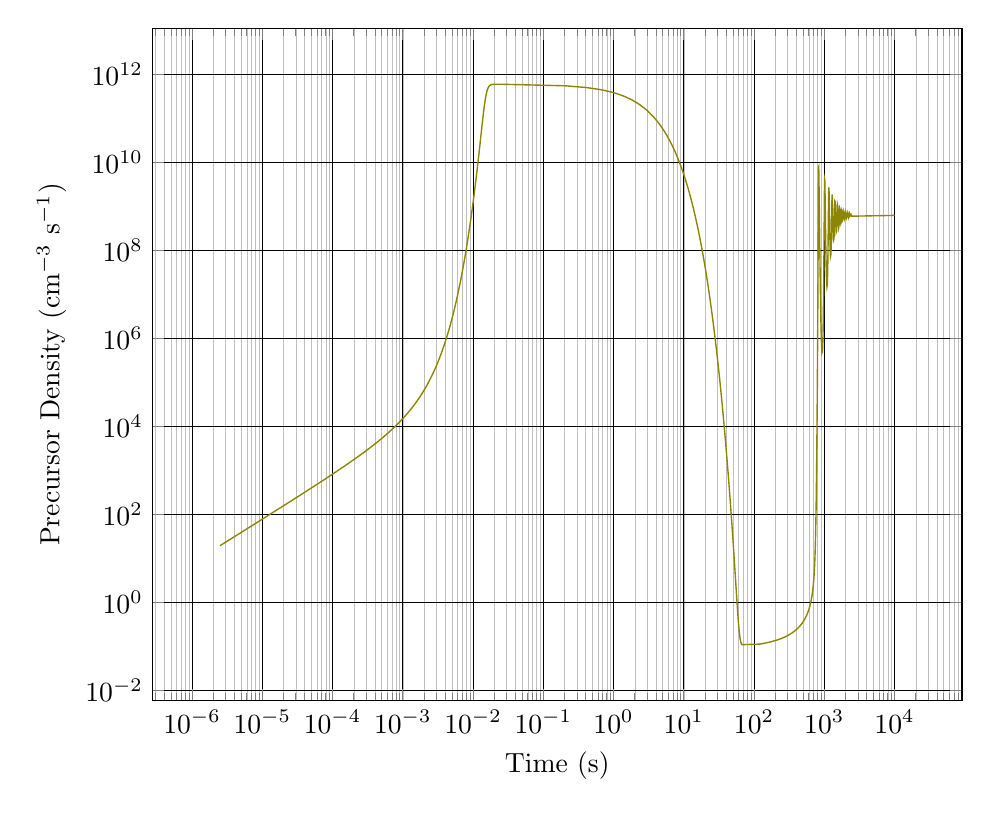
\begin{tikzpicture} \begin{loglogaxis}
[scale=1.5,
 grid=both, 
 major grid style={color=black,line width=0.2pt},
 minor grid style={color=gray!50,line width=0.1pt},
 xlabel=Time (s),
 ylabel=Precursor Density (cm$^{-3}$ s$^{-1}$)
]

\addplot[color=olive, line width=0.5pt] coordinates {
 ( 2.5e-06 , 19.0289 )
 ( 5e-06 , 38.1157 )
 ( 7.5e-06 , 57.2606 )
 ( 1e-05 , 76.4638 )
 ( 1.25e-05 , 95.7254 )
 ( 1.5e-05 , 115.046 )
 ( 1.75e-05 , 134.425 )
 ( 2e-05 , 153.863 )
 ( 2.25e-05 , 173.36 )
 ( 2.5e-05 , 192.916 )
 ( 2.75e-05 , 212.532 )
 ( 3.25e-05 , 251.944 )
 ( 3.75e-05 , 291.595 )
 ( 4.25e-05 , 331.488 )
 ( 4.75e-05 , 371.625 )
 ( 5.25e-05 , 412.006 )
 ( 5.7705e-05 , 454.304 )
 ( 6.34074e-05 , 500.952 )
 ( 6.96508e-05 , 552.399 )
 ( 7.64822e-05 , 609.139 )
 ( 8.39516e-05 , 671.72 )
 ( 9.21121e-05 , 740.746 )
 ( 0.00010102 , 816.881 )
 ( 0.000110736 , 900.863 )
 ( 0.000121322 , 993.504 )
 ( 0.000132845 , 1095.7 )
 ( 0.000145372 , 1208.45 )
 ( 0.000158974 , 1332.83 )
 ( 0.000173726 , 1470.07 )
 ( 0.000189702 , 1621.5 )
 ( 0.000206978 , 1788.6 )
 ( 0.00022563 , 1972.99 )
 ( 0.000245735 , 2176.49 )
 ( 0.000267368 , 2401.08 )
 ( 0.000290604 , 2648.96 )
 ( 0.000315511 , 2922.59 )
 ( 0.000342158 , 3224.64 )
 ( 0.000370606 , 3558.09 )
 ( 0.000400911 , 3926.24 )
 ( 0.000433125 , 4332.73 )
 ( 0.000467288 , 4781.57 )
 ( 0.000503434 , 5277.22 )
 ( 0.000541589 , 5824.58 )
 ( 0.000581768 , 6429.11 )
 ( 0.000623977 , 7096.81 )
 ( 0.000668212 , 7834.32 )
 ( 0.000714458 , 8648.99 )
 ( 0.000762693 , 9548.93 )
 ( 0.000812884 , 10543.1 )
 ( 0.000864989 , 11641.5 )
 ( 0.000918961 , 12855 )
 ( 0.000974741 , 14195.8 )
 ( 0.00103227 , 15677.3 )
 ( 0.00109148 , 17314.2 )
 ( 0.0011523 , 19123 )
 ( 0.00121465 , 21121.7 )
 ( 0.00127847 , 23330.4 )
 ( 0.00134367 , 25771.1 )
 ( 0.00141017 , 28468.2 )
 ( 0.0014779 , 31448.8 )
 ( 0.00154678 , 34742.6 )
 ( 0.00161674 , 38382.7 )
 ( 0.0016877 , 42405.5 )
 ( 0.00175959 , 46851.3 )
 ( 0.00183236 , 51764.5 )
 ( 0.00190592 , 57194.3 )
 ( 0.00198024 , 63195.2 )
 ( 0.00205523 , 69827.1 )
 ( 0.00213086 , 77156.5 )
 ( 0.00220707 , 85256.8 )
 ( 0.00228381 , 94209.1 )
 ( 0.00236104 , 104103 )
 ( 0.00243873 , 115037 )
 ( 0.00251682 , 127122 )
 ( 0.00259528 , 140478 )
 ( 0.00267409 , 155238 )
 ( 0.00275322 , 171552 )
 ( 0.00283262 , 189581 )
 ( 0.00291229 , 209506 )
 ( 0.00299219 , 231528 )
 ( 0.00307231 , 255866 )
 ( 0.00315263 , 282764 )
 ( 0.00323312 , 312492 )
 ( 0.00331378 , 345347 )
 ( 0.00339458 , 381658 )
 ( 0.00347551 , 421788 )
 ( 0.00355657 , 466140 )
 ( 0.00363774 , 515158 )
 ( 0.003719 , 569332 )
 ( 0.00380036 , 629204 )
 ( 0.0038818 , 695375 )
 ( 0.00396331 , 768506 )
 ( 0.00404489 , 849330 )
 ( 0.00412653 , 938657 )
 ( 0.00420823 , 1.03738e+06 )
 ( 0.00428998 , 1.14649e+06 )
 ( 0.00437177 , 1.26707e+06 )
 ( 0.00445361 , 1.40034e+06 )
 ( 0.00453548 , 1.54763e+06 )
 ( 0.00461738 , 1.71042e+06 )
 ( 0.00469932 , 1.89032e+06 )
 ( 0.00478128 , 2.08916e+06 )
 ( 0.00486327 , 2.3089e+06 )
 ( 0.00494528 , 2.55177e+06 )
 ( 0.00502731 , 2.82018e+06 )
 ( 0.00510936 , 3.11683e+06 )
 ( 0.00519143 , 3.44468e+06 )
 ( 0.00527351 , 3.80702e+06 )
 ( 0.00535561 , 4.20748e+06 )
 ( 0.00543772 , 4.65006e+06 )
 ( 0.00551984 , 5.1392e+06 )
 ( 0.00560197 , 5.6798e+06 )
 ( 0.00568411 , 6.27726e+06 )
 ( 0.00576626 , 6.93757e+06 )
 ( 0.00584841 , 7.66734e+06 )
 ( 0.00593057 , 8.47388e+06 )
 ( 0.00601274 , 9.36526e+06 )
 ( 0.00609492 , 1.03504e+07 )
 ( 0.0061771 , 1.14392e+07 )
 ( 0.00625928 , 1.26425e+07 )
 ( 0.00634147 , 1.39724e+07 )
 ( 0.00642367 , 1.54422e+07 )
 ( 0.00650586 , 1.70666e+07 )
 ( 0.00658806 , 1.88619e+07 )
 ( 0.00667027 , 2.0846e+07 )
 ( 0.00675247 , 2.30389e+07 )
 ( 0.00683468 , 2.54624e+07 )
 ( 0.00691689 , 2.81409e+07 )
 ( 0.00699911 , 3.11011e+07 )
 ( 0.00708132 , 3.43727e+07 )
 ( 0.00716354 , 3.79885e+07 )
 ( 0.00724576 , 4.19846e+07 )
 ( 0.00732798 , 4.64011e+07 )
 ( 0.0074102 , 5.12822e+07 )
 ( 0.00749243 , 5.66768e+07 )
 ( 0.00757465 , 6.26388e+07 )
 ( 0.00765688 , 6.9228e+07 )
 ( 0.00773911 , 7.65103e+07 )
 ( 0.00782134 , 8.45587e+07 )
 ( 0.00790357 , 9.34537e+07 )
 ( 0.00798581 , 1.03284e+08 )
 ( 0.00806805 , 1.14149e+08 )
 ( 0.00815028 , 1.26157e+08 )
 ( 0.00823252 , 1.39428e+08 )
 ( 0.00831477 , 1.54095e+08 )
 ( 0.00839701 , 1.70304e+08 )
 ( 0.00847926 , 1.88219e+08 )
 ( 0.00856151 , 2.08018e+08 )
 ( 0.00864377 , 2.299e+08 )
 ( 0.00872602 , 2.54084e+08 )
 ( 0.00880828 , 2.80812e+08 )
 ( 0.00889055 , 3.10351e+08 )
 ( 0.00897282 , 3.42998e+08 )
 ( 0.00905509 , 3.79079e+08 )
 ( 0.00913737 , 4.18955e+08 )
 ( 0.00921965 , 4.63025e+08 )
 ( 0.00930195 , 5.11732e+08 )
 ( 0.00938424 , 5.65561e+08 )
 ( 0.00946655 , 6.25053e+08 )
 ( 0.00954886 , 6.90803e+08 )
 ( 0.00963119 , 7.63469e+08 )
 ( 0.00971352 , 8.43779e+08 )
 ( 0.00979586 , 9.32535e+08 )
 ( 0.00987822 , 1.03063e+09 )
 ( 0.00996059 , 1.13904e+09 )
 ( 0.010043 , 1.25885e+09 )
 ( 0.0101254 , 1.39127e+09 )
 ( 0.0102078 , 1.53761e+09 )
 ( 0.0102902 , 1.69935e+09 )
 ( 0.0103727 , 1.87809e+09 )
 ( 0.0104552 , 2.07564e+09 )
 ( 0.0105377 , 2.29396e+09 )
 ( 0.0106203 , 2.53525e+09 )
 ( 0.0107029 , 2.80191e+09 )
 ( 0.0107855 , 3.09661e+09 )
 ( 0.0108681 , 3.42231e+09 )
 ( 0.0109508 , 3.78226e+09 )
 ( 0.0110336 , 4.18005e+09 )
 ( 0.0111164 , 4.61968e+09 )
 ( 0.0111993 , 5.10554e+09 )
 ( 0.0112823 , 5.64248e+09 )
 ( 0.0113653 , 6.23587e+09 )
 ( 0.0114484 , 6.89165e+09 )
 ( 0.0115316 , 7.61637e+09 )
 ( 0.0116149 , 8.41727e+09 )
 ( 0.0116983 , 9.30236e+09 )
 ( 0.0117819 , 1.02805e+10 )
 ( 0.0118656 , 1.13614e+10 )
 ( 0.0119494 , 1.25559e+10 )
 ( 0.0120334 , 1.38759e+10 )
 ( 0.0121177 , 1.53345e+10 )
 ( 0.0122021 , 1.69464e+10 )
 ( 0.0122868 , 1.87276e+10 )
 ( 0.0123717 , 2.06959e+10 )
 ( 0.0124569 , 2.28707e+10 )
 ( 0.0125425 , 2.52739e+10 )
 ( 0.0126284 , 2.79292e+10 )
 ( 0.0127147 , 3.08631e+10 )
 ( 0.0128015 , 3.41047e+10 )
 ( 0.0128888 , 3.76861e+10 )
 ( 0.0129767 , 4.16429e+10 )
 ( 0.0130652 , 4.60142e+10 )
 ( 0.0131544 , 5.08431e+10 )
 ( 0.0132444 , 5.61774e+10 )
 ( 0.0133354 , 6.20696e+10 )
 ( 0.0134273 , 6.85774e+10 )
 ( 0.0135204 , 7.57649e+10 )
 ( 0.0136148 , 8.37021e+10 )
 ( 0.0137107 , 9.24664e+10 )
 ( 0.0138083 , 1.02143e+11 )
 ( 0.0139079 , 1.12825e+11 )
 ( 0.0140096 , 1.24615e+11 )
 ( 0.014114 , 1.37626e+11 )
 ( 0.0142214 , 1.51981e+11 )
 ( 0.0143324 , 1.67814e+11 )
 ( 0.0144475 , 1.85272e+11 )
 ( 0.0145676 , 2.04514e+11 )
 ( 0.0146938 , 2.25712e+11 )
 ( 0.0148273 , 2.49049e+11 )
 ( 0.0149701 , 2.7472e+11 )
 ( 0.0151246 , 3.02927e+11 )
 ( 0.0152944 , 3.33873e+11 )
 ( 0.015485 , 3.67749e+11 )
 ( 0.0157049 , 4.04707e+11 )
 ( 0.0159259 , 4.38594e+11 )
 ( 0.0161754 , 4.72168e+11 )
 ( 0.0163828 , 4.96042e+11 )
 ( 0.0165675 , 5.14279e+11 )
 ( 0.0167379 , 5.28717e+11 )
 ( 0.0168984 , 5.40393e+11 )
 ( 0.0170516 , 5.49969e+11 )
 ( 0.0171994 , 5.57902e+11 )
 ( 0.0173429 , 5.64522e+11 )
 ( 0.017483 , 5.70075e+11 )
 ( 0.0176205 , 5.74754e+11 )
 ( 0.0177558 , 5.78709e+11 )
 ( 0.0178893 , 5.82061e+11 )
 ( 0.0180214 , 5.84907e+11 )
 ( 0.0181522 , 5.87328e+11 )
 ( 0.0182821 , 5.89389e+11 )
 ( 0.0184113 , 5.91146e+11 )
 ( 0.0185397 , 5.92645e+11 )
 ( 0.0186677 , 5.93923e+11 )
 ( 0.0187953 , 5.95013e+11 )
 ( 0.0189227 , 5.95944e+11 )
 ( 0.0190499 , 5.96738e+11 )
 ( 0.019177 , 5.97414e+11 )
 ( 0.0193041 , 5.9799e+11 )
 ( 0.0194313 , 5.98481e+11 )
 ( 0.0195588 , 5.98897e+11 )
 ( 0.0196865 , 5.9925e+11 )
 ( 0.0198147 , 5.99549e+11 )
 ( 0.0199434 , 5.99801e+11 )
 ( 0.0200728 , 6.00013e+11 )
 ( 0.020203 , 6.0019e+11 )
 ( 0.0203343 , 6.00337e+11 )
 ( 0.0204667 , 6.00459e+11 )
 ( 0.0206007 , 6.00559e+11 )
 ( 0.0207364 , 6.00639e+11 )
 ( 0.0208743 , 6.00702e+11 )
 ( 0.0210148 , 6.00751e+11 )
 ( 0.0211585 , 6.00787e+11 )
 ( 0.021306 , 6.00812e+11 )
 ( 0.0214584 , 6.00827e+11 )
 ( 0.0216167 , 6.00833e+11 )
 ( 0.0217825 , 6.0083e+11 )
 ( 0.021958 , 6.00819e+11 )
 ( 0.0221463 , 6.00799e+11 )
 ( 0.0223519 , 6.00772e+11 )
 ( 0.0225819 , 6.00734e+11 )
 ( 0.0228484 , 6.00683e+11 )
 ( 0.0231746 , 6.00614e+11 )
 ( 0.0236127 , 6.00514e+11 )
 ( 0.0243294 , 6.00339e+11 )
 ( 0.0267446 , 5.99718e+11 )
 ( 0.202966 , 5.55272e+11 )
 ( 0.410704 , 5.06426e+11 )
 ( 0.674763 , 4.4976e+11 )
 ( 0.953514 , 3.96198e+11 )
 ( 1.23378 , 3.48343e+11 )
 ( 1.5155 , 3.0576e+11 )
 ( 1.79858 , 2.67996e+11 )
 ( 2.08293 , 2.34603e+11 )
 ( 2.36843 , 2.05147e+11 )
 ( 2.65497 , 1.79219e+11 )
 ( 2.94247 , 1.56437e+11 )
 ( 3.23083 , 1.36451e+11 )
 ( 3.51998 , 1.18941e+11 )
 ( 3.80984 , 1.0362e+11 )
 ( 4.10034 , 9.02265e+10 )
 ( 4.39142 , 7.85293e+10 )
 ( 4.68303 , 6.83216e+10 )
 ( 4.97513 , 5.94199e+10 )
 ( 5.26766 , 5.16618e+10 )
 ( 5.5606 , 4.49042e+10 )
 ( 5.8539 , 3.90209e+10 )
 ( 6.14754 , 3.39008e+10 )
 ( 6.44149 , 2.94467e+10 )
 ( 6.73572 , 2.55732e+10 )
 ( 7.03022 , 2.22057e+10 )
 ( 7.32496 , 1.92789e+10 )
 ( 7.61993 , 1.67356e+10 )
 ( 7.91511 , 1.45261e+10 )
 ( 8.21048 , 1.26069e+10 )
 ( 8.50603 , 1.09403e+10 )
 ( 8.80176 , 9.49309e+09 )
 ( 9.09765 , 8.23667e+09 )
 ( 9.39369 , 7.14601e+09 )
 ( 9.68987 , 6.19934e+09 )
 ( 9.98619 , 5.37774e+09 )
 ( 10.2826 , 4.66475e+09 )
 ( 10.5792 , 4.04608e+09 )
 ( 10.8759 , 3.50928e+09 )
 ( 11.1727 , 3.04355e+09 )
 ( 11.4696 , 2.63952e+09 )
 ( 11.7666 , 2.28903e+09 )
 ( 12.0638 , 1.985e+09 )
 ( 12.361 , 1.72129e+09 )
 ( 12.6583 , 1.49256e+09 )
 ( 12.9557 , 1.29418e+09 )
 ( 13.2532 , 1.12214e+09 )
 ( 13.5508 , 9.72934e+08 )
 ( 13.8484 , 8.43545e+08 )
 ( 14.1462 , 7.31343e+08 )
 ( 14.444 , 6.34049e+08 )
 ( 14.7419 , 5.49684e+08 )
 ( 15.0399 , 4.76533e+08 )
 ( 15.338 , 4.13106e+08 )
 ( 15.6361 , 3.58114e+08 )
 ( 15.9343 , 3.10435e+08 )
 ( 16.2326 , 2.69098e+08 )
 ( 16.531 , 2.3326e+08 )
 ( 16.8294 , 2.02191e+08 )
 ( 17.1279 , 1.75257e+08 )
 ( 17.4265 , 1.51907e+08 )
 ( 17.7251 , 1.31666e+08 )
 ( 18.0238 , 1.14119e+08 )
 ( 18.3226 , 9.89093e+07 )
 ( 18.6215 , 8.57248e+07 )
 ( 18.9204 , 7.42964e+07 )
 ( 19.2194 , 6.43904e+07 )
 ( 19.5185 , 5.58041e+07 )
 ( 19.8176 , 4.83619e+07 )
 ( 20.1168 , 4.19115e+07 )
 ( 20.4161 , 3.63207e+07 )
 ( 20.7154 , 3.14752e+07 )
 ( 21.0148 , 2.72756e+07 )
 ( 21.3143 , 2.36359e+07 )
 ( 21.6138 , 2.04816e+07 )
 ( 21.9134 , 1.77479e+07 )
 ( 22.2131 , 1.53788e+07 )
 ( 22.5128 , 1.33257e+07 )
 ( 22.8126 , 1.15465e+07 )
 ( 23.1125 , 1.00047e+07 )
 ( 23.4124 , 8.66865e+06 )
 ( 23.7124 , 7.51087e+06 )
 ( 24.0125 , 6.50761e+06 )
 ( 24.3126 , 5.63827e+06 )
 ( 24.6128 , 4.88498e+06 )
 ( 24.9131 , 4.23226e+06 )
 ( 25.2134 , 3.6667e+06 )
 ( 25.5138 , 3.17666e+06 )
 ( 25.8142 , 2.75207e+06 )
 ( 26.1148 , 2.38419e+06 )
 ( 26.4153 , 2.06546e+06 )
 ( 26.716 , 1.7893e+06 )
 ( 27.0167 , 1.55005e+06 )
 ( 27.3175 , 1.34277e+06 )
 ( 27.6183 , 1.16318e+06 )
 ( 27.9192 , 1.00761e+06 )
 ( 28.2201 , 872823 )
 ( 28.5212 , 756059 )
 ( 28.8222 , 654907 )
 ( 29.1234 , 567281 )
 ( 29.4246 , 491373 )
 ( 29.7258 , 425618 )
 ( 30.0271 , 368658 )
 ( 30.3284 , 319318 )
 ( 30.6298 , 276579 )
 ( 30.9313 , 239559 )
 ( 31.2328 , 207492 )
 ( 31.5343 , 179718 )
 ( 31.8359 , 155661 )
 ( 32.1374 , 134824 )
 ( 32.4391 , 116777 )
 ( 32.7407 , 101146 )
 ( 33.0423 , 87608.4 )
 ( 33.344 , 75883.7 )
 ( 33.6456 , 65729.4 )
 ( 33.9472 , 56935.2 )
 ( 34.2488 , 49319.2 )
 ( 34.5504 , 42723.5 )
 ( 34.8518 , 37011.6 )
 ( 35.1532 , 32065.2 )
 ( 35.4545 , 27781.6 )
 ( 35.7557 , 24072.2 )
 ( 36.0566 , 20860.1 )
 ( 36.3574 , 18078.5 )
 ( 36.658 , 15669.9 )
 ( 36.9582 , 13584.2 )
 ( 37.2581 , 11778.2 )
 ( 37.5577 , 10214.4 )
 ( 37.8567 , 8860.22 )
 ( 38.1553 , 7687.66 )
 ( 38.4532 , 6672.33 )
 ( 38.7504 , 5793.13 )
 ( 39.0468 , 5031.79 )
 ( 39.3423 , 4372.49 )
 ( 39.6368 , 3801.53 )
 ( 39.93 , 3307.03 )
 ( 40.2219 , 2878.71 )
 ( 40.5124 , 2507.68 )
 ( 40.8012 , 2186.2 )
 ( 41.0882 , 1907.62 )
 ( 41.3731 , 1666.14 )
 ( 41.6424 , 1466.16 )
 ( 41.8814 , 1308.86 )
 ( 42.1303 , 1162.96 )
 ( 42.3834 , 1031.32 )
 ( 42.6394 , 913.342 )
 ( 42.872 , 817.88 )
 ( 43.1174 , 727.964 )
 ( 43.3491 , 652.161 )
 ( 43.5901 , 581.708 )
 ( 43.8124 , 523.477 )
 ( 44.0431 , 469.23 )
 ( 44.2788 , 419.59 )
 ( 44.5162 , 374.912 )
 ( 44.7528 , 335.129 )
 ( 44.9866 , 299.956 )
 ( 45.2164 , 269.002 )
 ( 45.441 , 241.831 )
 ( 45.6729 , 216.662 )
 ( 45.8963 , 194.894 )
 ( 46.1222 , 175.109 )
 ( 46.3481 , 157.342 )
 ( 46.5718 , 141.518 )
 ( 46.8001 , 127.014 )
 ( 47.0297 , 113.928 )
 ( 47.2581 , 102.249 )
 ( 47.4836 , 91.8982 )
 ( 47.7102 , 82.5519 )
 ( 47.9356 , 74.2008 )
 ( 48.1624 , 66.6505 )
 ( 48.3882 , 59.8989 )
 ( 48.6112 , 53.9046 )
 ( 48.8366 , 48.456 )
 ( 49.0618 , 43.5651 )
 ( 49.2873 , 39.1618 )
 ( 49.5111 , 35.2342 )
 ( 49.7359 , 31.6865 )
 ( 49.9594 , 28.5144 )
 ( 50.1835 , 25.6539 )
 ( 50.4076 , 23.0811 )
 ( 50.6313 , 20.7726 )
 ( 50.8551 , 18.6939 )
 ( 51.0796 , 16.8197 )
 ( 51.3046 , 15.1303 )
 ( 51.5291 , 13.6152 )
 ( 51.7539 , 12.2513 )
 ( 51.9785 , 11.0258 )
 ( 52.204 , 9.92 )
 ( 52.4295 , 8.92593 )
 ( 52.655 , 8.03277 )
 ( 52.8807 , 7.22919 )
 ( 53.1068 , 6.50608 )
 ( 53.3334 , 5.85456 )
 ( 53.5604 , 5.26849 )
 ( 53.7878 , 4.74134 )
 ( 54.0157 , 4.26682 )
 ( 54.2443 , 3.83973 )
 ( 54.4734 , 3.45558 )
 ( 54.7031 , 3.10999 )
 ( 54.9336 , 2.79892 )
 ( 55.165 , 2.51896 )
 ( 55.3975 , 2.26694 )
 ( 55.6311 , 2.04012 )
 ( 55.8658 , 1.8361 )
 ( 56.1021 , 1.65239 )
 ( 56.3399 , 1.4871 )
 ( 56.5794 , 1.33835 )
 ( 56.8209 , 1.20452 )
 ( 57.0647 , 1.08405 )
 ( 57.3111 , 0.975622 )
 ( 57.5603 , 0.878034 )
 ( 57.813 , 0.790206 )
 ( 58.0693 , 0.711171 )
 ( 58.33 , 0.640048 )
 ( 58.5958 , 0.576028 )
 ( 58.8673 , 0.518416 )
 ( 59.1455 , 0.466571 )
 ( 59.4317 , 0.419905 )
 ( 59.7271 , 0.377913 )
 ( 60.0337 , 0.340117 )
 ( 60.3536 , 0.306104 )
 ( 60.6898 , 0.275492 )
 ( 61.0462 , 0.247939 )
 ( 61.4281 , 0.223143 )
 ( 61.8431 , 0.200827 )
 ( 62.3022 , 0.180743 )
 ( 62.8232 , 0.162667 )
 ( 63.4364 , 0.1464 )
 ( 64.2006 , 0.13176 )
 ( 65.2575 , 0.118583 )
 ( 67.1495 , 0.106725 )
 ( 119.948 , 0.109733 )
 ( 162.656 , 0.120681 )
 ( 203.061 , 0.132719 )
 ( 241.207 , 0.145954 )
 ( 277.142 , 0.160506 )
 ( 310.926 , 0.176503 )
 ( 342.624 , 0.194089 )
 ( 372.309 , 0.21342 )
 ( 400.057 , 0.234668 )
 ( 425.951 , 0.258021 )
 ( 450.074 , 0.283687 )
 ( 472.512 , 0.311891 )
 ( 493.353 , 0.342882 )
 ( 512.686 , 0.376932 )
 ( 530.597 , 0.414338 )
 ( 547.172 , 0.455428 )
 ( 562.497 , 0.500557 )
 ( 576.653 , 0.550117 )
 ( 589.72 , 0.604535 )
 ( 601.775 , 0.66428 )
 ( 612.891 , 0.729861 )
 ( 623.138 , 0.801837 )
 ( 632.582 , 0.880821 )
 ( 641.287 , 0.967481 )
 ( 649.31 , 1.06254 )
 ( 656.708 , 1.1668 )
 ( 663.533 , 1.28113 )
 ( 669.833 , 1.4065 )
 ( 675.653 , 1.54392 )
 ( 681.033 , 1.69456 )
 ( 686.014 , 1.85963 )
 ( 690.629 , 2.04051 )
 ( 694.913 , 2.2387 )
 ( 698.893 , 2.4558 )
 ( 702.598 , 2.69363 )
 ( 706.051 , 2.95411 )
 ( 709.277 , 3.23945 )
 ( 712.295 , 3.55202 )
 ( 715.123 , 3.89425 )
 ( 717.777 , 4.26895 )
 ( 720.275 , 4.67941 )
 ( 722.63 , 5.12904 )
 ( 724.854 , 5.62151 )
 ( 726.956 , 6.16065 )
 ( 728.949 , 6.75134 )
 ( 730.839 , 7.39757 )
 ( 732.636 , 8.1054 )
 ( 734.35 , 8.8812 )
 ( 735.983 , 9.73011 )
 ( 737.546 , 10.6609 )
 ( 739.04 , 11.6795 )
 ( 740.472 , 12.7953 )
 ( 741.849 , 14.0197 )
 ( 743.171 , 15.3591 )
 ( 744.446 , 16.8307 )
 ( 745.677 , 18.4445 )
 ( 746.864 , 20.2141 )
 ( 748.006 , 22.1442 )
 ( 749.111 , 24.2606 )
 ( 750.184 , 26.5841 )
 ( 751.23 , 29.1492 )
 ( 752.248 , 31.9718 )
 ( 753.236 , 35.0681 )
 ( 754.194 , 38.4567 )
 ( 755.123 , 42.1626 )
 ( 756.028 , 46.2264 )
 ( 756.916 , 50.7177 )
 ( 757.773 , 55.5987 )
 ( 758.612 , 60.9638 )
 ( 759.45 , 66.9976 )
 ( 760.244 , 73.4182 )
 ( 761.052 , 80.7517 )
 ( 761.824 , 88.6365 )
 ( 762.591 , 97.4292 )
 ( 763.343 , 107.111 )
 ( 764.066 , 117.55 )
 ( 764.813 , 129.657 )
 ( 765.503 , 142.211 )
 ( 766.196 , 156.329 )
 ( 766.886 , 172.083 )
 ( 767.563 , 189.402 )
 ( 768.21 , 207.937 )
 ( 768.966 , 232.388 )
 ( 769.688 , 258.978 )
 ( 770.336 , 285.944 )
 ( 771.136 , 323.871 )
 ( 771.769 , 358.092 )
 ( 772.392 , 395.925 )
 ( 773.004 , 437.751 )
 ( 773.608 , 483.992 )
 ( 774.202 , 535.112 )
 ( 774.787 , 591.627 )
 ( 775.364 , 654.106 )
 ( 775.932 , 723.177 )
 ( 776.493 , 799.536 )
 ( 777.046 , 883.951 )
 ( 777.591 , 977.272 )
 ( 778.13 , 1080.44 )
 ( 778.661 , 1194.49 )
 ( 779.186 , 1320.57 )
 ( 779.704 , 1459.95 )
 ( 780.216 , 1614.03 )
 ( 780.721 , 1784.36 )
 ( 781.221 , 1972.66 )
 ( 781.715 , 2180.82 )
 ( 782.203 , 2410.93 )
 ( 782.686 , 2665.31 )
 ( 783.163 , 2946.51 )
 ( 783.635 , 3257.37 )
 ( 784.103 , 3601.01 )
 ( 784.565 , 3980.88 )
 ( 785.022 , 4400.81 )
 ( 785.475 , 4865.02 )
 ( 785.924 , 5378.17 )
 ( 786.367 , 5945.42 )
 ( 786.807 , 6572.49 )
 ( 787.242 , 7265.66 )
 ( 787.673 , 8031.92 )
 ( 788.1 , 8878.95 )
 ( 788.523 , 9815.28 )
 ( 788.943 , 10850.3 )
 ( 789.358 , 11994.5 )
 ( 789.77 , 13259.2 )
 ( 790.178 , 14657.3 )
 ( 790.583 , 16201.1 )
 ( 790.982 , 17903.1 )
 ( 791.378 , 19779.5 )
 ( 791.77 , 21848.4 )
 ( 792.157 , 24129.5 )
 ( 792.541 , 26644.8 )
 ( 792.922 , 29418.4 )
 ( 793.299 , 32476.8 )
 ( 793.672 , 35849.5 )
 ( 794.043 , 39568.7 )
 ( 794.41 , 43670.3 )
 ( 794.775 , 48193.6 )
 ( 795.136 , 53181.9 )
 ( 795.495 , 58683.4 )
 ( 795.85 , 64750.8 )
 ( 796.203 , 71442.4 )
 ( 796.554 , 78822.7 )
 ( 796.902 , 86962.4 )
 ( 797.247 , 95940 )
 ( 797.59 , 105842 )
 ( 797.93 , 116763 )
 ( 798.269 , 128809 )
 ( 798.604 , 142095 )
 ( 798.938 , 156750 )
 ( 799.269 , 172914 )
 ( 799.598 , 190743 )
 ( 799.925 , 210409 )
 ( 800.25 , 232101 )
 ( 800.573 , 256028 )
 ( 800.893 , 282422 )
 ( 801.212 , 311535 )
 ( 801.529 , 343649 )
 ( 801.844 , 379073 )
 ( 802.157 , 418149 )
 ( 802.468 , 461253 )
 ( 802.777 , 508801 )
 ( 803.084 , 561253 )
 ( 803.39 , 619113 )
 ( 803.693 , 682940 )
 ( 803.995 , 753350 )
 ( 804.296 , 831022 )
 ( 804.594 , 916706 )
 ( 804.891 , 1.01123e+06 )
 ( 805.186 , 1.1155e+06 )
 ( 805.48 , 1.23054e+06 )
 ( 805.772 , 1.35744e+06 )
 ( 806.063 , 1.49744e+06 )
 ( 806.351 , 1.65188e+06 )
 ( 806.639 , 1.82227e+06 )
 ( 806.925 , 2.01024e+06 )
 ( 807.209 , 2.21761e+06 )
 ( 807.492 , 2.44639e+06 )
 ( 807.773 , 2.6988e+06 )
 ( 808.053 , 2.97726e+06 )
 ( 808.332 , 3.28447e+06 )
 ( 808.609 , 3.62341e+06 )
 ( 808.884 , 3.99735e+06 )
 ( 809.159 , 4.40991e+06 )
 ( 809.432 , 4.86509e+06 )
 ( 809.703 , 5.36729e+06 )
 ( 809.973 , 5.92138e+06 )
 ( 810.242 , 6.53272e+06 )
 ( 810.51 , 7.20724e+06 )
 ( 810.777 , 7.95146e+06 )
 ( 811.042 , 8.77261e+06 )
 ( 811.306 , 9.67865e+06 )
 ( 811.569 , 1.06784e+07 )
 ( 811.83 , 1.17815e+07 )
 ( 812.09 , 1.29987e+07 )
 ( 812.35 , 1.43417e+07 )
 ( 812.608 , 1.58238e+07 )
 ( 812.865 , 1.74592e+07 )
 ( 813.121 , 1.92639e+07 )
 ( 813.375 , 2.12554e+07 )
 ( 813.629 , 2.34532e+07 )
 ( 813.882 , 2.58785e+07 )
 ( 814.133 , 2.85552e+07 )
 ( 814.384 , 3.15093e+07 )
 ( 814.633 , 3.47697e+07 )
 ( 814.882 , 3.83682e+07 )
 ( 815.13 , 4.23401e+07 )
 ( 815.377 , 4.67243e+07 )
 ( 815.623 , 5.15637e+07 )
 ( 815.868 , 5.69061e+07 )
 ( 816.112 , 6.28038e+07 )
 ( 816.356 , 6.93152e+07 )
 ( 816.598 , 7.65044e+07 )
 ( 816.84 , 8.44426e+07 )
 ( 817.082 , 9.32085e+07 )
 ( 817.322 , 1.02889e+08 )
 ( 817.562 , 1.13581e+08 )
 ( 817.802 , 1.25392e+08 )
 ( 818.041 , 1.38439e+08 )
 ( 818.28 , 1.52854e+08 )
 ( 818.518 , 1.68783e+08 )
 ( 818.756 , 1.86388e+08 )
 ( 818.994 , 2.05847e+08 )
 ( 819.231 , 2.27362e+08 )
 ( 819.469 , 2.51153e+08 )
 ( 819.706 , 2.77467e+08 )
 ( 819.944 , 3.06581e+08 )
 ( 820.182 , 3.388e+08 )
 ( 820.42 , 3.74437e+08 )
 ( 820.659 , 4.13817e+08 )
 ( 820.897 , 4.57333e+08 )
 ( 821.136 , 5.05416e+08 )
 ( 821.376 , 5.58546e+08 )
 ( 821.616 , 6.1725e+08 )
 ( 821.857 , 6.8211e+08 )
 ( 822.099 , 7.53768e+08 )
 ( 822.342 , 8.32932e+08 )
 ( 822.587 , 9.20385e+08 )
 ( 822.833 , 1.01699e+09 )
 ( 823.082 , 1.12369e+09 )
 ( 823.333 , 1.24154e+09 )
 ( 823.588 , 1.37169e+09 )
 ( 823.845 , 1.5154e+09 )
 ( 824.107 , 1.67407e+09 )
 ( 824.373 , 1.84924e+09 )
 ( 824.645 , 2.04259e+09 )
 ( 824.923 , 2.25596e+09 )
 ( 825.209 , 2.49138e+09 )
 ( 825.504 , 2.75105e+09 )
 ( 825.81 , 3.03737e+09 )
 ( 826.129 , 3.35295e+09 )
 ( 826.463 , 3.7006e+09 )
 ( 826.817 , 4.08331e+09 )
 ( 827.195 , 4.50423e+09 )
 ( 827.604 , 4.96657e+09 )
 ( 828.056 , 5.47337e+09 )
 ( 828.566 , 6.0271e+09 )
 ( 829.514 , 6.94563e+09 )
 ( 831.003 , 7.92451e+09 )
 ( 833.734 , 8.02686e+09 )
 ( 835.288 , 7.34613e+09 )
 ( 836.564 , 6.58906e+09 )
 ( 837.717 , 5.8466e+09 )
 ( 838.799 , 5.15179e+09 )
 ( 839.836 , 4.51651e+09 )
 ( 840.842 , 3.94479e+09 )
 ( 841.826 , 3.43499e+09 )
 ( 842.794 , 2.9842e+09 )
 ( 843.751 , 2.58737e+09 )
 ( 844.7 , 2.23992e+09 )
 ( 845.645 , 1.9364e+09 )
 ( 846.585 , 1.6723e+09 )
 ( 847.526 , 1.44272e+09 )
 ( 848.465 , 1.24379e+09 )
 ( 849.407 , 1.07144e+09 )
 ( 850.35 , 9.22539e+08 )
 ( 851.295 , 7.94027e+08 )
 ( 852.242 , 6.83436e+08 )
 ( 853.191 , 5.88262e+08 )
 ( 854.142 , 5.06354e+08 )
 ( 855.098 , 4.35859e+08 )
 ( 856.059 , 3.75185e+08 )
 ( 857.024 , 3.22963e+08 )
 ( 857.997 , 2.78014e+08 )
 ( 858.975 , 2.39324e+08 )
 ( 859.962 , 2.06021e+08 )
 ( 860.956 , 1.77355e+08 )
 ( 861.959 , 1.52679e+08 )
 ( 862.97 , 1.31438e+08 )
 ( 863.992 , 1.13153e+08 )
 ( 865.024 , 9.74136e+07 )
 ( 866.067 , 8.38642e+07 )
 ( 867.121 , 7.22002e+07 )
 ( 868.188 , 6.21592e+07 )
 ( 869.267 , 5.35153e+07 )
 ( 870.36 , 4.6074e+07 )
 ( 871.467 , 3.9668e+07 )
 ( 872.59 , 3.41531e+07 )
 ( 873.728 , 2.94053e+07 )
 ( 874.884 , 2.53179e+07 )
 ( 876.057 , 2.17991e+07 )
 ( 877.249 , 1.87696e+07 )
 ( 878.462 , 1.61615e+07 )
 ( 879.696 , 1.3916e+07 )
 ( 880.953 , 1.19828e+07 )
 ( 882.235 , 1.03184e+07 )
 ( 883.543 , 8.88539e+06 )
 ( 884.879 , 7.65162e+06 )
 ( 886.246 , 6.58938e+06 )
 ( 887.646 , 5.67479e+06 )
 ( 889.083 , 4.88734e+06 )
 ( 890.559 , 4.20934e+06 )
 ( 892.078 , 3.62559e+06 )
 ( 893.646 , 3.12296e+06 )
 ( 895.268 , 2.69019e+06 )
 ( 896.95 , 2.31757e+06 )
 ( 898.701 , 1.99676e+06 )
 ( 900.53 , 1.72053e+06 )
 ( 902.452 , 1.48273e+06 )
 ( 904.483 , 1.278e+06 )
 ( 906.646 , 1.1018e+06 )
 ( 908.968 , 950474 )
 ( 911.498 , 820435 )
 ( 914.287 , 709649 )
 ( 917.498 , 614268 )
 ( 921.304 , 534664 )
 ( 926.632 , 467859 )
 ( 943.148 , 509247 )
 ( 946.018 , 558869 )
 ( 948.338 , 613744 )
 ( 950.327 , 674063 )
 ( 952.094 , 740458 )
 ( 953.701 , 813576 )
 ( 955.182 , 894109 )
 ( 956.563 , 982817 )
 ( 957.86 , 1.08053e+06 )
 ( 959.087 , 1.18817e+06 )
 ( 960.254 , 1.30674e+06 )
 ( 961.367 , 1.43735e+06 )
 ( 962.434 , 1.58123e+06 )
 ( 963.46 , 1.73972e+06 )
 ( 964.447 , 1.91432e+06 )
 ( 965.402 , 2.10667e+06 )
 ( 966.325 , 2.31857e+06 )
 ( 967.22 , 2.55201e+06 )
 ( 968.089 , 2.80921e+06 )
 ( 968.933 , 3.09257e+06 )
 ( 969.756 , 3.40476e+06 )
 ( 970.558 , 3.74874e+06 )
 ( 971.34 , 4.12776e+06 )
 ( 972.104 , 4.54538e+06 )
 ( 972.852 , 5.00556e+06 )
 ( 973.583 , 5.51265e+06 )
 ( 974.298 , 6.07145e+06 )
 ( 975 , 6.68726e+06 )
 ( 975.688 , 7.3659e+06 )
 ( 976.363 , 8.11381e+06 )
 ( 977.026 , 8.9381e+06 )
 ( 977.677 , 9.84658e+06 )
 ( 978.317 , 1.08479e+07 )
 ( 978.947 , 1.19516e+07 )
 ( 979.566 , 1.31681e+07 )
 ( 980.176 , 1.45091e+07 )
 ( 980.776 , 1.59873e+07 )
 ( 981.368 , 1.76169e+07 )
 ( 981.951 , 1.94134e+07 )
 ( 982.526 , 2.13939e+07 )
 ( 983.093 , 2.35774e+07 )
 ( 983.652 , 2.59849e+07 )
 ( 984.205 , 2.86394e+07 )
 ( 984.75 , 3.15665e+07 )
 ( 985.289 , 3.47941e+07 )
 ( 985.822 , 3.83535e+07 )
 ( 986.348 , 4.22788e+07 )
 ( 986.869 , 4.6608e+07 )
 ( 987.384 , 5.1383e+07 )
 ( 987.893 , 5.66499e+07 )
 ( 988.398 , 6.246e+07 )
 ( 988.897 , 6.88696e+07 )
 ( 989.392 , 7.59412e+07 )
 ( 989.882 , 8.3744e+07 )
 ( 990.368 , 9.23543e+07 )
 ( 990.851 , 1.01857e+08 )
 ( 991.329 , 1.12345e+08 )
 ( 991.804 , 1.23922e+08 )
 ( 992.275 , 1.36704e+08 )
 ( 992.743 , 1.50818e+08 )
 ( 993.209 , 1.66404e+08 )
 ( 993.672 , 1.83621e+08 )
 ( 994.132 , 2.02641e+08 )
 ( 994.591 , 2.23659e+08 )
 ( 995.048 , 2.46889e+08 )
 ( 995.504 , 2.72572e+08 )
 ( 995.958 , 3.00975e+08 )
 ( 996.412 , 3.32397e+08 )
 ( 996.866 , 3.67169e+08 )
 ( 997.321 , 4.05665e+08 )
 ( 997.776 , 4.48304e+08 )
 ( 998.231 , 4.95449e+08 )
 ( 998.688 , 5.47536e+08 )
 ( 999.145 , 6.05079e+08 )
 ( 999.604 , 6.68643e+08 )
 ( 1000.07 , 7.38854e+08 )
 ( 1000.53 , 8.16398e+08 )
 ( 1001 , 9.02033e+08 )
 ( 1001.47 , 9.9659e+08 )
 ( 1001.96 , 1.10098e+09 )
 ( 1002.44 , 1.21621e+09 )
 ( 1002.94 , 1.34338e+09 )
 ( 1003.45 , 1.48368e+09 )
 ( 1003.98 , 1.63843e+09 )
 ( 1004.52 , 1.80903e+09 )
 ( 1005.09 , 1.99703e+09 )
 ( 1005.68 , 2.20403e+09 )
 ( 1006.31 , 2.43177e+09 )
 ( 1006.98 , 2.68195e+09 )
 ( 1007.72 , 2.95621e+09 )
 ( 1008.55 , 3.25577e+09 )
 ( 1010.07 , 3.75163e+09 )
 ( 1012.55 , 4.26659e+09 )
 ( 1016.87 , 4.12684e+09 )
 ( 1019.04 , 3.68983e+09 )
 ( 1020.82 , 3.25745e+09 )
 ( 1022.4 , 2.85708e+09 )
 ( 1023.89 , 2.49356e+09 )
 ( 1025.31 , 2.16987e+09 )
 ( 1026.69 , 1.8826e+09 )
 ( 1028.04 , 1.63076e+09 )
 ( 1029.38 , 1.40963e+09 )
 ( 1030.7 , 1.21745e+09 )
 ( 1032.02 , 1.0497e+09 )
 ( 1033.33 , 9.04739e+08 )
 ( 1034.66 , 7.79018e+08 )
 ( 1035.98 , 6.70802e+08 )
 ( 1037.31 , 5.77426e+08 )
 ( 1038.64 , 4.97071e+08 )
 ( 1039.99 , 4.27923e+08 )
 ( 1041.36 , 3.68412e+08 )
 ( 1042.74 , 3.17193e+08 )
 ( 1044.14 , 2.73107e+08 )
 ( 1045.56 , 2.35161e+08 )
 ( 1047.01 , 2.02496e+08 )
 ( 1048.49 , 1.74377e+08 )
 ( 1050.01 , 1.50171e+08 )
 ( 1051.56 , 1.29332e+08 )
 ( 1053.16 , 1.11392e+08 )
 ( 1054.8 , 9.59475e+07 )
 ( 1056.5 , 8.26506e+07 )
 ( 1058.26 , 7.12031e+07 )
 ( 1060.1 , 6.13475e+07 )
 ( 1062.02 , 5.28632e+07 )
 ( 1064.04 , 4.55593e+07 )
 ( 1066.18 , 3.92727e+07 )
 ( 1068.47 , 3.38677e+07 )
 ( 1070.94 , 2.92235e+07 )
 ( 1073.65 , 2.52576e+07 )
 ( 1076.71 , 2.18437e+07 )
 ( 1080.26 , 1.89719e+07 )
 ( 1084.87 , 1.65255e+07 )
 ( 1092.4 , 1.47951e+07 )
 ( 1102.85 , 1.63597e+07 )
 ( 1106.03 , 1.79281e+07 )
 ( 1108.53 , 1.96685e+07 )
 ( 1110.65 , 2.15999e+07 )
 ( 1112.52 , 2.37251e+07 )
 ( 1114.21 , 2.60657e+07 )
 ( 1115.77 , 2.86443e+07 )
 ( 1117.21 , 3.14855e+07 )
 ( 1118.57 , 3.46166e+07 )
 ( 1119.85 , 3.80671e+07 )
 ( 1121.07 , 4.18699e+07 )
 ( 1122.23 , 4.60612e+07 )
 ( 1123.35 , 5.06809e+07 )
 ( 1124.42 , 5.57731e+07 )
 ( 1125.46 , 6.13866e+07 )
 ( 1126.46 , 6.75752e+07 )
 ( 1127.43 , 7.43985e+07 )
 ( 1128.38 , 8.19223e+07 )
 ( 1129.3 , 9.02195e+07 )
 ( 1130.19 , 9.93705e+07 )
 ( 1131.07 , 1.09465e+08 )
 ( 1131.93 , 1.20601e+08 )
 ( 1132.77 , 1.32888e+08 )
 ( 1133.59 , 1.46448e+08 )
 ( 1134.4 , 1.61416e+08 )
 ( 1135.2 , 1.77941e+08 )
 ( 1135.99 , 1.96188e+08 )
 ( 1136.77 , 2.16343e+08 )
 ( 1137.53 , 2.38611e+08 )
 ( 1138.29 , 2.6322e+08 )
 ( 1139.05 , 2.90427e+08 )
 ( 1139.79 , 3.20516e+08 )
 ( 1140.54 , 3.53807e+08 )
 ( 1141.28 , 3.90656e+08 )
 ( 1142.02 , 4.31466e+08 )
 ( 1142.76 , 4.76687e+08 )
 ( 1143.5 , 5.26794e+08 )
 ( 1144.24 , 5.82164e+08 )
 ( 1144.99 , 6.4331e+08 )
 ( 1145.74 , 7.10823e+08 )
 ( 1146.5 , 7.85353e+08 )
 ( 1147.27 , 8.67612e+08 )
 ( 1148.05 , 9.58374e+08 )
 ( 1148.85 , 1.05849e+09 )
 ( 1149.67 , 1.16886e+09 )
 ( 1150.52 , 1.29049e+09 )
 ( 1151.41 , 1.4244e+09 )
 ( 1152.35 , 1.5717e+09 )
 ( 1153.35 , 1.73345e+09 )
 ( 1154.44 , 1.91062e+09 )
 ( 1155.68 , 2.1038e+09 )
 ( 1158 , 2.42123e+09 )
 ( 1162.42 , 2.71326e+09 )
 ( 1166.39 , 2.58487e+09 )
 ( 1168.58 , 2.38643e+09 )
 ( 1171.14 , 2.0978e+09 )
 ( 1173.35 , 1.83113e+09 )
 ( 1175.38 , 1.59312e+09 )
 ( 1177.31 , 1.38092e+09 )
 ( 1179.17 , 1.19536e+09 )
 ( 1181.02 , 1.03194e+09 )
 ( 1182.83 , 8.90488e+08 )
 ( 1184.65 , 7.67038e+08 )
 ( 1186.46 , 6.60978e+08 )
 ( 1188.29 , 5.69182e+08 )
 ( 1190.14 , 4.9013e+08 )
 ( 1192.02 , 4.22048e+08 )
 ( 1193.95 , 3.63469e+08 )
 ( 1195.93 , 3.13063e+08 )
 ( 1197.97 , 2.69687e+08 )
 ( 1200.09 , 2.3236e+08 )
 ( 1202.31 , 2.00237e+08 )
 ( 1204.66 , 1.72598e+08 )
 ( 1207.17 , 1.4882e+08 )
 ( 1209.89 , 1.28374e+08 )
 ( 1212.9 , 1.10807e+08 )
 ( 1216.35 , 9.57481e+07 )
 ( 1220.51 , 8.29547e+07 )
 ( 1226.32 , 7.23767e+07 )
 ( 1244.16 , 7.98334e+07 )
 ( 1247.15 , 8.76501e+07 )
 ( 1249.59 , 9.62605e+07 )
 ( 1251.72 , 1.0576e+08 )
 ( 1253.63 , 1.16243e+08 )
 ( 1255.38 , 1.27813e+08 )
 ( 1257.01 , 1.40584e+08 )
 ( 1258.54 , 1.5468e+08 )
 ( 1260 , 1.70241e+08 )
 ( 1261.39 , 1.87423e+08 )
 ( 1262.72 , 2.06399e+08 )
 ( 1264.01 , 2.27361e+08 )
 ( 1265.26 , 2.50524e+08 )
 ( 1266.48 , 2.76126e+08 )
 ( 1267.68 , 3.04436e+08 )
 ( 1268.85 , 3.35753e+08 )
 ( 1270 , 3.70413e+08 )
 ( 1271.14 , 4.08795e+08 )
 ( 1272.28 , 4.51323e+08 )
 ( 1273.41 , 4.9848e+08 )
 ( 1274.54 , 5.50756e+08 )
 ( 1275.68 , 6.08621e+08 )
 ( 1276.82 , 6.72474e+08 )
 ( 1277.98 , 7.4291e+08 )
 ( 1279.16 , 8.20574e+08 )
 ( 1280.37 , 9.06156e+08 )
 ( 1281.62 , 1.00039e+09 )
 ( 1282.92 , 1.10404e+09 )
 ( 1284.32 , 1.21785e+09 )
 ( 1285.83 , 1.34247e+09 )
 ( 1287.52 , 1.47824e+09 )
 ( 1290.73 , 1.70051e+09 )
 ( 1297.5 , 1.8784e+09 )
 ( 1302.69 , 1.71937e+09 )
 ( 1306.42 , 1.50518e+09 )
 ( 1309.45 , 1.30996e+09 )
 ( 1312.2 , 1.13601e+09 )
 ( 1314.8 , 9.82499e+08 )
 ( 1317.33 , 8.48094e+08 )
 ( 1319.85 , 7.30807e+08 )
 ( 1322.37 , 6.29155e+08 )
 ( 1324.91 , 5.41733e+08 )
 ( 1327.52 , 4.666e+08 )
 ( 1330.21 , 4.02015e+08 )
 ( 1333.04 , 3.46495e+08 )
 ( 1336.05 , 2.9878e+08 )
 ( 1339.34 , 2.57799e+08 )
 ( 1343.03 , 2.22662e+08 )
 ( 1347.41 , 1.92676e+08 )
 ( 1353.27 , 1.6759e+08 )
 ( 1374.42 , 1.79907e+08 )
 ( 1377.72 , 1.97746e+08 )
 ( 1380.45 , 2.17433e+08 )
 ( 1382.85 , 2.39195e+08 )
 ( 1385.04 , 2.6326e+08 )
 ( 1387.07 , 2.8988e+08 )
 ( 1388.99 , 3.19335e+08 )
 ( 1390.82 , 3.51941e+08 )
 ( 1392.58 , 3.8805e+08 )
 ( 1394.3 , 4.28065e+08 )
 ( 1396 , 4.72438e+08 )
 ( 1397.67 , 5.21685e+08 )
 ( 1399.35 , 5.76394e+08 )
 ( 1401.03 , 6.36888e+08 )
 ( 1402.74 , 7.03534e+08 )
 ( 1404.48 , 7.76897e+08 )
 ( 1406.29 , 8.57554e+08 )
 ( 1408.2 , 9.46057e+08 )
 ( 1410.26 , 1.04285e+09 )
 ( 1412.58 , 1.14805e+09 )
 ( 1417.09 , 1.31819e+09 )
 ( 1432.59 , 1.27009e+09 )
 ( 1437.08 , 1.10556e+09 )
 ( 1440.9 , 9.57222e+08 )
 ( 1444.42 , 8.27635e+08 )
 ( 1447.86 , 7.13241e+08 )
 ( 1451.27 , 6.14988e+08 )
 ( 1454.76 , 5.29862e+08 )
 ( 1458.4 , 4.56705e+08 )
 ( 1462.31 , 3.93975e+08 )
 ( 1466.68 , 3.40279e+08 )
 ( 1471.9 , 2.94602e+08 )
 ( 1479.2 , 2.56962e+08 )
 ( 1498.77 , 2.72819e+08 )
 ( 1503.02 , 3.00242e+08 )
 ( 1506.42 , 3.30485e+08 )
 ( 1509.4 , 3.63964e+08 )
 ( 1512.12 , 4.01063e+08 )
 ( 1514.68 , 4.42204e+08 )
 ( 1517.13 , 4.87863e+08 )
 ( 1519.53 , 5.38529e+08 )
 ( 1521.91 , 5.94576e+08 )
 ( 1524.31 , 6.5658e+08 )
 ( 1526.78 , 7.24949e+08 )
 ( 1529.35 , 7.99868e+08 )
 ( 1532.13 , 8.81622e+08 )
 ( 1535.27 , 9.70043e+08 )
 ( 1541.75 , 1.10901e+09 )
 ( 1557.99 , 1.03569e+09 )
 ( 1563.95 , 8.96497e+08 )
 ( 1568.89 , 7.75486e+08 )
 ( 1573.63 , 6.68243e+08 )
 ( 1578.32 , 5.76693e+08 )
 ( 1583.27 , 4.97477e+08 )
 ( 1588.78 , 4.29793e+08 )
 ( 1595.56 , 3.72724e+08 )
 ( 1606.93 , 3.2973e+08 )
 ( 1622.02 , 3.61362e+08 )
 ( 1627.34 , 3.98397e+08 )
 ( 1631.57 , 4.39151e+08 )
 ( 1635.31 , 4.84311e+08 )
 ( 1638.8 , 5.34232e+08 )
 ( 1642.18 , 5.89361e+08 )
 ( 1645.57 , 6.50219e+08 )
 ( 1649.09 , 7.17307e+08 )
 ( 1652.89 , 7.9038e+08 )
 ( 1659.93 , 9.08595e+08 )
 ( 1684.63 , 8.48155e+08 )
 ( 1691.86 , 7.31674e+08 )
 ( 1698.34 , 6.3147e+08 )
 ( 1705.01 , 5.44776e+08 )
 ( 1712.59 , 4.71431e+08 )
 ( 1723.35 , 4.12458e+08 )
 ( 1745.47 , 4.39819e+08 )
 ( 1751.94 , 4.85605e+08 )
 ( 1757.23 , 5.35934e+08 )
 ( 1762.09 , 5.91357e+08 )
 ( 1766.9 , 6.5222e+08 )
 ( 1771.99 , 7.1876e+08 )
 ( 1781.54 , 8.24469e+08 )
 ( 1807.58 , 7.69871e+08 )
 ( 1817.17 , 6.64774e+08 )
 ( 1826.28 , 5.73825e+08 )
 ( 1836.93 , 4.98234e+08 )
 ( 1876.47 , 5.50049e+08 )
 ( 1883.38 , 6.06707e+08 )
 ( 1890.2 , 6.68143e+08 )
 ( 1902.92 , 7.65012e+08 )
 ( 1933.05 , 6.99298e+08 )
 ( 1945.63 , 6.04704e+08 )
 ( 1960.08 , 5.26594e+08 )
 ( 1999.28 , 5.81703e+08 )
 ( 2008.75 , 6.40517e+08 )
 ( 2026.11 , 7.29376e+08 )
 ( 2060.43 , 6.47802e+08 )
 ( 2078.27 , 5.6421e+08 )
 ( 2130.04 , 6.35311e+08 )
 ( 2154.88 , 7.06574e+08 )
 ( 2183.14 , 6.39123e+08 )
 ( 2209.44 , 5.63751e+08 )
 ( 2248.43 , 6.20731e+08 )
 ( 2277.9 , 6.82886e+08 )
 ( 2317.9 , 6.03378e+08 )
 ( 2397.9 , 6.65598e+08 )
 ( 2447.9 , 5.98523e+08 )
 ( 10000, 6.24117e+08 )
};
\end{loglogaxis}
\end{tikzpicture}
\caption{Precursor density for fission reactor kinetics example.}
 \label{Fig:ode_precursorDensity}
\end{center}
\end{figure}


\begin{figure}[htp!]
\begin{center}
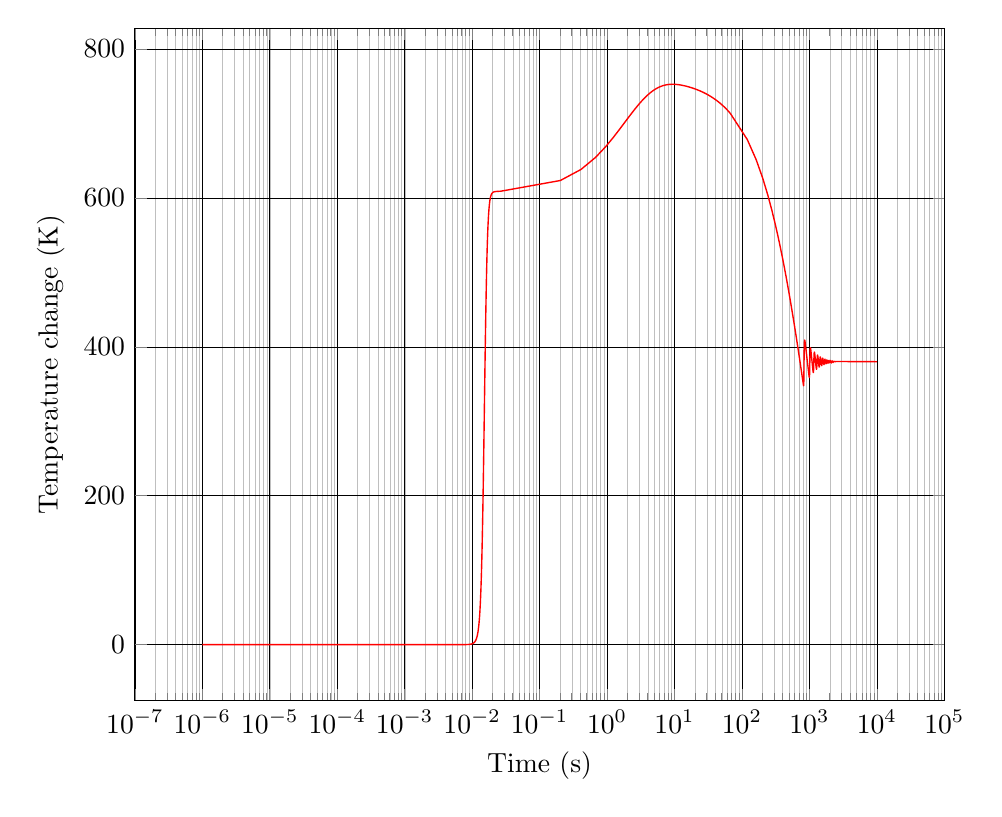
\begin{tikzpicture} \begin{semilogxaxis}
[scale=1.5,
 grid=both, 
 major grid style={color=black,line width=0.2pt},
 minor grid style={color=gray!50,line width=0.1pt},
 xlabel=Time (s),
 ylabel=Temperature change (K)
]

\addplot[color=red, line width=0.5pt] coordinates {
 ( 1.0e-06, 0 ) 
 ( 2.5e-06 , 1.91942e-08 )
 ( 5e-06 , 3.84469e-08 )
 ( 7.5e-06 , 5.77582e-08 )
 ( 1e-05 , 7.71283e-08 )
 ( 1.25e-05 , 9.65574e-08 )
 ( 1.5e-05 , 1.16046e-07 )
 ( 1.75e-05 , 1.35593e-07 )
 ( 2e-05 , 1.552e-07 )
 ( 2.25e-05 , 1.74867e-07 )
 ( 2.5e-05 , 1.94594e-07 )
 ( 2.75e-05 , 2.1438e-07 )
 ( 3.25e-05 , 2.54135e-07 )
 ( 3.75e-05 , 2.94132e-07 )
 ( 4.25e-05 , 3.34372e-07 )
 ( 4.75e-05 , 3.74858e-07 )
 ( 5.25e-05 , 4.15591e-07 )
 ( 5.7705e-05 , 4.58259e-07 )
 ( 6.34074e-05 , 5.05314e-07 )
 ( 6.96508e-05 , 5.57209e-07 )
 ( 7.64822e-05 , 6.14445e-07 )
 ( 8.39516e-05 , 6.77572e-07 )
 ( 9.21121e-05 , 7.47201e-07 )
 ( 0.00010102 , 8.24002e-07 )
 ( 0.000110736 , 9.08718e-07 )
 ( 0.000121322 , 1.00217e-06 )
 ( 0.000132845 , 1.10526e-06 )
 ( 0.000145372 , 1.219e-06 )
 ( 0.000158974 , 1.34447e-06 )
 ( 0.000173726 , 1.48292e-06 )
 ( 0.000189702 , 1.63568e-06 )
 ( 0.000206978 , 1.80424e-06 )
 ( 0.00022563 , 1.99026e-06 )
 ( 0.000245735 , 2.19554e-06 )
 ( 0.000267368 , 2.42211e-06 )
 ( 0.000290604 , 2.67219e-06 )
 ( 0.000315511 , 2.94823e-06 )
 ( 0.000342158 , 3.25295e-06 )
 ( 0.000370606 , 3.58936e-06 )
 ( 0.000400911 , 3.96077e-06 )
 ( 0.000433125 , 4.37087e-06 )
 ( 0.000467288 , 4.8237e-06 )
 ( 0.000503434 , 5.32376e-06 )
 ( 0.000541589 , 5.87601e-06 )
 ( 0.000581768 , 6.48593e-06 )
 ( 0.000623977 , 7.15959e-06 )
 ( 0.000668212 , 7.9037e-06 )
 ( 0.000714458 , 8.72567e-06 )
 ( 0.000762693 , 9.63369e-06 )
 ( 0.000812884 , 1.06368e-05 )
 ( 0.000864989 , 1.17451e-05 )
 ( 0.000918961 , 1.29695e-05 )
 ( 0.000974741 , 1.43224e-05 )
 ( 0.00103227 , 1.58172e-05 )
 ( 0.00109148 , 1.7469e-05 )
 ( 0.0011523 , 1.92941e-05 )
 ( 0.00121465 , 2.13109e-05 )
 ( 0.00127847 , 2.35396e-05 )
 ( 0.00134367 , 2.60024e-05 )
 ( 0.00141017 , 2.8724e-05 )
 ( 0.0014779 , 3.17317e-05 )
 ( 0.00154678 , 3.50555e-05 )
 ( 0.00161674 , 3.87287e-05 )
 ( 0.0016877 , 4.27881e-05 )
 ( 0.00175959 , 4.72743e-05 )
 ( 0.00183236 , 5.22323e-05 )
 ( 0.00190592 , 5.77117e-05 )
 ( 0.00198024 , 6.37672e-05 )
 ( 0.00205523 , 7.04597e-05 )
 ( 0.00213086 , 7.7856e-05 )
 ( 0.00220707 , 8.60303e-05 )
 ( 0.00228381 , 9.50643e-05 )
 ( 0.00236104 , 0.000105049 )
 ( 0.00243873 , 0.000116083 )
 ( 0.00251682 , 0.000128278 )
 ( 0.00259528 , 0.000141756 )
 ( 0.00267409 , 0.000156652 )
 ( 0.00275322 , 0.000173114 )
 ( 0.00283262 , 0.000191308 )
 ( 0.00291229 , 0.000211416 )
 ( 0.00299219 , 0.000233639 )
 ( 0.00307231 , 0.0002582 )
 ( 0.00315263 , 0.000285345 )
 ( 0.00323312 , 0.000315345 )
 ( 0.00331378 , 0.000348501 )
 ( 0.00339458 , 0.000385144 )
 ( 0.00347551 , 0.000425642 )
 ( 0.00355657 , 0.0004704 )
 ( 0.00363774 , 0.000519867 )
 ( 0.003719 , 0.000574537 )
 ( 0.00380036 , 0.000634958 )
 ( 0.0038818 , 0.000701735 )
 ( 0.00396331 , 0.000775536 )
 ( 0.00404489 , 0.000857101 )
 ( 0.00412653 , 0.000947246 )
 ( 0.00420823 , 0.00104687 )
 ( 0.00428998 , 0.00115698 )
 ( 0.00437177 , 0.00127867 )
 ( 0.00445361 , 0.00141316 )
 ( 0.00453548 , 0.0015618 )
 ( 0.00461738 , 0.00172608 )
 ( 0.00469932 , 0.00190763 )
 ( 0.00478128 , 0.00210829 )
 ( 0.00486327 , 0.00233005 )
 ( 0.00494528 , 0.00257514 )
 ( 0.00502731 , 0.00284601 )
 ( 0.00510936 , 0.00314538 )
 ( 0.00519143 , 0.00347624 )
 ( 0.00527351 , 0.0038419 )
 ( 0.00535561 , 0.00424603 )
 ( 0.00543772 , 0.00469267 )
 ( 0.00551984 , 0.00518629 )
 ( 0.00560197 , 0.00573184 )
 ( 0.00568411 , 0.00633478 )
 ( 0.00576626 , 0.00700114 )
 ( 0.00584841 , 0.0077376 )
 ( 0.00593057 , 0.00855153 )
 ( 0.00601274 , 0.00945108 )
 ( 0.00609492 , 0.0104453 )
 ( 0.0061771 , 0.011544 )
 ( 0.00625928 , 0.0127584 )
 ( 0.00634147 , 0.0141005 )
 ( 0.00642367 , 0.0155837 )
 ( 0.00650586 , 0.017223 )
 ( 0.00658806 , 0.0190348 )
 ( 0.00667027 , 0.0210371 )
 ( 0.00675247 , 0.02325 )
 ( 0.00683468 , 0.0256958 )
 ( 0.00691689 , 0.0283988 )
 ( 0.00699911 , 0.0313862 )
 ( 0.00708132 , 0.0346878 )
 ( 0.00716354 , 0.0383367 )
 ( 0.00724576 , 0.0423694 )
 ( 0.00732798 , 0.0468264 )
 ( 0.0074102 , 0.0517523 )
 ( 0.00749243 , 0.0571963 )
 ( 0.00757465 , 0.0632129 )
 ( 0.00765688 , 0.0698625 )
 ( 0.00773911 , 0.0772116 )
 ( 0.00782134 , 0.0853337 )
 ( 0.00790357 , 0.0943103 )
 ( 0.00798581 , 0.104231 )
 ( 0.00806805 , 0.115195 )
 ( 0.00815028 , 0.127313 )
 ( 0.00823252 , 0.140706 )
 ( 0.00831477 , 0.155507 )
 ( 0.00839701 , 0.171865 )
 ( 0.00847926 , 0.189944 )
 ( 0.00856151 , 0.209925 )
 ( 0.00864377 , 0.232008 )
 ( 0.00872602 , 0.256413 )
 ( 0.00880828 , 0.283386 )
 ( 0.00889055 , 0.313196 )
 ( 0.00897282 , 0.346142 )
 ( 0.00905509 , 0.382553 )
 ( 0.00913737 , 0.422795 )
 ( 0.00921965 , 0.46727 )
 ( 0.00930195 , 0.516422 )
 ( 0.00938424 , 0.570746 )
 ( 0.00946655 , 0.630783 )
 ( 0.00954886 , 0.697136 )
 ( 0.00963119 , 0.770468 )
 ( 0.00971352 , 0.851513 )
 ( 0.00979586 , 0.941084 )
 ( 0.00987822 , 1.04008 )
 ( 0.00996059 , 1.14948 )
 ( 0.010043 , 1.27039 )
 ( 0.0101254 , 1.40402 )
 ( 0.0102078 , 1.55171 )
 ( 0.0102902 , 1.71492 )
 ( 0.0103727 , 1.89531 )
 ( 0.0104552 , 2.09467 )
 ( 0.0105377 , 2.31499 )
 ( 0.0106203 , 2.55849 )
 ( 0.0107029 , 2.82759 )
 ( 0.0107855 , 3.125 )
 ( 0.0108681 , 3.45368 )
 ( 0.0109508 , 3.81693 )
 ( 0.0110336 , 4.21838 )
 ( 0.0111164 , 4.66204 )
 ( 0.0111993 , 5.15235 )
 ( 0.0112823 , 5.69421 )
 ( 0.0113653 , 6.29305 )
 ( 0.0114484 , 6.95484 )
 ( 0.0115316 , 7.68621 )
 ( 0.0116149 , 8.49446 )
 ( 0.0116983 , 9.38766 )
 ( 0.0117819 , 10.3748 )
 ( 0.0118656 , 11.4656 )
 ( 0.0119494 , 12.671 )
 ( 0.0120334 , 14.0031 )
 ( 0.0121177 , 15.4752 )
 ( 0.0122021 , 17.1019 )
 ( 0.0122868 , 18.8994 )
 ( 0.0123717 , 20.8857 )
 ( 0.0124569 , 23.0806 )
 ( 0.0125425 , 25.5058 )
 ( 0.0126284 , 28.1855 )
 ( 0.0127147 , 31.1464 )
 ( 0.0128015 , 34.4178 )
 ( 0.0128888 , 38.0321 )
 ( 0.0129767 , 42.0253 )
 ( 0.0130652 , 46.4368 )
 ( 0.0131544 , 51.3103 )
 ( 0.0132444 , 56.6937 )
 ( 0.0133354 , 62.6402 )
 ( 0.0134273 , 69.2081 )
 ( 0.0135204 , 76.4618 )
 ( 0.0136148 , 84.4724 )
 ( 0.0137107 , 93.3178 )
 ( 0.0138083 , 103.084 )
 ( 0.0139079 , 113.865 )
 ( 0.0140096 , 125.765 )
 ( 0.014114 , 138.897 )
 ( 0.0142214 , 153.385 )
 ( 0.0143324 , 169.366 )
 ( 0.0144475 , 186.988 )
 ( 0.0145676 , 206.411 )
 ( 0.0146938 , 227.808 )
 ( 0.0148273 , 251.367 )
 ( 0.0149701 , 277.282 )
 ( 0.0151246 , 305.76 )
 ( 0.0152944 , 337.007 )
 ( 0.015485 , 371.216 )
 ( 0.0157049 , 408.545 )
 ( 0.0159259 , 442.78 )
 ( 0.0161754 , 476.712 )
 ( 0.0163828 , 500.851 )
 ( 0.0165675 , 519.302 )
 ( 0.0167379 , 533.916 )
 ( 0.0168984 , 545.743 )
 ( 0.0170516 , 555.452 )
 ( 0.0171994 , 563.501 )
 ( 0.0173429 , 570.225 )
 ( 0.017483 , 575.873 )
 ( 0.0176205 , 580.639 )
 ( 0.0177558 , 584.673 )
 ( 0.0178893 , 588.099 )
 ( 0.0180214 , 591.015 )
 ( 0.0181522 , 593.502 )
 ( 0.0182821 , 595.625 )
 ( 0.0184113 , 597.442 )
 ( 0.0185397 , 598.997 )
 ( 0.0186677 , 600.331 )
 ( 0.0187953 , 601.475 )
 ( 0.0189227 , 602.458 )
 ( 0.0190499 , 603.303 )
 ( 0.019177 , 604.029 )
 ( 0.0193041 , 604.655 )
 ( 0.0194313 , 605.193 )
 ( 0.0195588 , 605.658 )
 ( 0.0196865 , 606.058 )
 ( 0.0198147 , 606.405 )
 ( 0.0199434 , 606.704 )
 ( 0.0200728 , 606.962 )
 ( 0.020203 , 607.187 )
 ( 0.0203343 , 607.381 )
 ( 0.0204667 , 607.55 )
 ( 0.0206007 , 607.697 )
 ( 0.0207364 , 607.826 )
 ( 0.0208743 , 607.938 )
 ( 0.0210148 , 608.036 )
 ( 0.0211585 , 608.123 )
 ( 0.021306 , 608.2 )
 ( 0.0214584 , 608.268 )
 ( 0.0216167 , 608.329 )
 ( 0.0217825 , 608.384 )
 ( 0.021958 , 608.434 )
 ( 0.0221463 , 608.48 )
 ( 0.0223519 , 608.524 )
 ( 0.0225819 , 608.566 )
 ( 0.0228484 , 608.608 )
 ( 0.0231746 , 608.653 )
 ( 0.0236127 , 608.705 )
 ( 0.0243294 , 608.778 )
 ( 0.0267446 , 608.995 )
 ( 0.202966 , 623.331 )
 ( 0.410704 , 638.153 )
 ( 0.674763 , 654.32 )
 ( 0.953514 , 668.74 )
 ( 1.23378 , 681.009 )
 ( 1.5155 , 691.49 )
 ( 1.79858 , 700.468 )
 ( 2.08293 , 708.173 )
 ( 2.36843 , 714.794 )
 ( 2.65497 , 720.487 )
 ( 2.94247 , 725.383 )
 ( 3.23083 , 729.593 )
 ( 3.51998 , 733.212 )
 ( 3.80984 , 736.32 )
 ( 4.10034 , 738.987 )
 ( 4.39142 , 741.272 )
 ( 4.68303 , 743.225 )
 ( 4.97513 , 744.893 )
 ( 5.26766 , 746.311 )
 ( 5.5606 , 747.514 )
 ( 5.8539 , 748.53 )
 ( 6.14754 , 749.384 )
 ( 6.44149 , 750.097 )
 ( 6.73572 , 750.687 )
 ( 7.03022 , 751.172 )
 ( 7.32496 , 751.564 )
 ( 7.61993 , 751.877 )
 ( 7.91511 , 752.12 )
 ( 8.21048 , 752.303 )
 ( 8.50603 , 752.433 )
 ( 8.80176 , 752.518 )
 ( 9.09765 , 752.564 )
 ( 9.39369 , 752.575 )
 ( 9.68987 , 752.557 )
 ( 9.98619 , 752.512 )
 ( 10.2826 , 752.446 )
 ( 10.5792 , 752.359 )
 ( 10.8759 , 752.256 )
 ( 11.1727 , 752.139 )
 ( 11.4696 , 752.008 )
 ( 11.7666 , 751.867 )
 ( 12.0638 , 751.716 )
 ( 12.361 , 751.556 )
 ( 12.6583 , 751.39 )
 ( 12.9557 , 751.217 )
 ( 13.2532 , 751.039 )
 ( 13.5508 , 750.856 )
 ( 13.8484 , 750.669 )
 ( 14.1462 , 750.478 )
 ( 14.444 , 750.284 )
 ( 14.7419 , 750.088 )
 ( 15.0399 , 749.889 )
 ( 15.338 , 749.689 )
 ( 15.6361 , 749.486 )
 ( 15.9343 , 749.282 )
 ( 16.2326 , 749.077 )
 ( 16.531 , 748.87 )
 ( 16.8294 , 748.663 )
 ( 17.1279 , 748.455 )
 ( 17.4265 , 748.246 )
 ( 17.7251 , 748.036 )
 ( 18.0238 , 747.826 )
 ( 18.3226 , 747.616 )
 ( 18.6215 , 747.405 )
 ( 18.9204 , 747.193 )
 ( 19.2194 , 746.981 )
 ( 19.5185 , 746.77 )
 ( 19.8176 , 746.557 )
 ( 20.1168 , 746.345 )
 ( 20.4161 , 746.132 )
 ( 20.7154 , 745.92 )
 ( 21.0148 , 745.707 )
 ( 21.3143 , 745.494 )
 ( 21.6138 , 745.281 )
 ( 21.9134 , 745.068 )
 ( 22.2131 , 744.855 )
 ( 22.5128 , 744.642 )
 ( 22.8126 , 744.428 )
 ( 23.1125 , 744.215 )
 ( 23.4124 , 744.002 )
 ( 23.7124 , 743.789 )
 ( 24.0125 , 743.575 )
 ( 24.3126 , 743.362 )
 ( 24.6128 , 743.149 )
 ( 24.9131 , 742.935 )
 ( 25.2134 , 742.722 )
 ( 25.5138 , 742.508 )
 ( 25.8142 , 742.295 )
 ( 26.1148 , 742.082 )
 ( 26.4153 , 741.868 )
 ( 26.716 , 741.655 )
 ( 27.0167 , 741.442 )
 ( 27.3175 , 741.228 )
 ( 27.6183 , 741.015 )
 ( 27.9192 , 740.802 )
 ( 28.2201 , 740.588 )
 ( 28.5212 , 740.375 )
 ( 28.8222 , 740.162 )
 ( 29.1234 , 739.949 )
 ( 29.4246 , 739.735 )
 ( 29.7258 , 739.522 )
 ( 30.0271 , 739.309 )
 ( 30.3284 , 739.096 )
 ( 30.6298 , 738.883 )
 ( 30.9313 , 738.67 )
 ( 31.2328 , 738.457 )
 ( 31.5343 , 738.244 )
 ( 31.8359 , 738.031 )
 ( 32.1374 , 737.818 )
 ( 32.4391 , 737.605 )
 ( 32.7407 , 737.392 )
 ( 33.0423 , 737.179 )
 ( 33.344 , 736.966 )
 ( 33.6456 , 736.754 )
 ( 33.9472 , 736.541 )
 ( 34.2488 , 736.328 )
 ( 34.5504 , 736.116 )
 ( 34.8518 , 735.904 )
 ( 35.1532 , 735.691 )
 ( 35.4545 , 735.479 )
 ( 35.7557 , 735.267 )
 ( 36.0566 , 735.056 )
 ( 36.3574 , 734.844 )
 ( 36.658 , 734.633 )
 ( 36.9582 , 734.422 )
 ( 37.2581 , 734.211 )
 ( 37.5577 , 734.001 )
 ( 37.8567 , 733.791 )
 ( 38.1553 , 733.581 )
 ( 38.4532 , 733.372 )
 ( 38.7504 , 733.163 )
 ( 39.0468 , 732.955 )
 ( 39.3423 , 732.748 )
 ( 39.6368 , 732.542 )
 ( 39.93 , 732.336 )
 ( 40.2219 , 732.132 )
 ( 40.5124 , 731.928 )
 ( 40.8012 , 731.726 )
 ( 41.0882 , 731.525 )
 ( 41.3731 , 731.326 )
 ( 41.6424 , 731.137 )
 ( 41.8814 , 730.97 )
 ( 42.1303 , 730.796 )
 ( 42.3834 , 730.619 )
 ( 42.6394 , 730.44 )
 ( 42.872 , 730.277 )
 ( 43.1174 , 730.106 )
 ( 43.3491 , 729.944 )
 ( 43.5901 , 729.776 )
 ( 43.8124 , 729.62 )
 ( 44.0431 , 729.459 )
 ( 44.2788 , 729.295 )
 ( 44.5162 , 729.129 )
 ( 44.7528 , 728.964 )
 ( 44.9866 , 728.801 )
 ( 45.2164 , 728.641 )
 ( 45.441 , 728.484 )
 ( 45.6729 , 728.323 )
 ( 45.8963 , 728.167 )
 ( 46.1222 , 728.01 )
 ( 46.3481 , 727.852 )
 ( 46.5718 , 727.696 )
 ( 46.8001 , 727.537 )
 ( 47.0297 , 727.378 )
 ( 47.2581 , 727.219 )
 ( 47.4836 , 727.062 )
 ( 47.7102 , 726.904 )
 ( 47.9356 , 726.747 )
 ( 48.1624 , 726.59 )
 ( 48.3882 , 726.433 )
 ( 48.6112 , 726.278 )
 ( 48.8366 , 726.121 )
 ( 49.0618 , 725.965 )
 ( 49.2873 , 725.808 )
 ( 49.5111 , 725.652 )
 ( 49.7359 , 725.496 )
 ( 49.9594 , 725.341 )
 ( 50.1835 , 725.186 )
 ( 50.4076 , 725.03 )
 ( 50.6313 , 724.875 )
 ( 50.8551 , 724.72 )
 ( 51.0796 , 724.564 )
 ( 51.3046 , 724.408 )
 ( 51.5291 , 724.253 )
 ( 51.7539 , 724.097 )
 ( 51.9785 , 723.941 )
 ( 52.204 , 723.785 )
 ( 52.4295 , 723.629 )
 ( 52.655 , 723.473 )
 ( 52.8807 , 723.316 )
 ( 53.1068 , 723.16 )
 ( 53.3334 , 723.003 )
 ( 53.5604 , 722.846 )
 ( 53.7878 , 722.689 )
 ( 54.0157 , 722.531 )
 ( 54.2443 , 722.373 )
 ( 54.4734 , 722.215 )
 ( 54.7031 , 722.056 )
 ( 54.9336 , 721.897 )
 ( 55.165 , 721.737 )
 ( 55.3975 , 721.576 )
 ( 55.6311 , 721.415 )
 ( 55.8658 , 721.253 )
 ( 56.1021 , 721.09 )
 ( 56.3399 , 720.926 )
 ( 56.5794 , 720.761 )
 ( 56.8209 , 720.594 )
 ( 57.0647 , 720.426 )
 ( 57.3111 , 720.256 )
 ( 57.5603 , 720.085 )
 ( 57.813 , 719.91 )
 ( 58.0693 , 719.734 )
 ( 58.33 , 719.554 )
 ( 58.5958 , 719.371 )
 ( 58.8673 , 719.184 )
 ( 59.1455 , 718.993 )
 ( 59.4317 , 718.796 )
 ( 59.7271 , 718.593 )
 ( 60.0337 , 718.382 )
 ( 60.3536 , 718.162 )
 ( 60.6898 , 717.931 )
 ( 61.0462 , 717.687 )
 ( 61.4281 , 717.424 )
 ( 61.8431 , 717.139 )
 ( 62.3022 , 716.824 )
 ( 62.8232 , 716.467 )
 ( 63.4364 , 716.047 )
 ( 64.2006 , 715.523 )
 ( 65.2575 , 714.8 )
 ( 67.1495 , 713.507 )
 ( 119.948 , 678.353 )
 ( 162.656 , 651.188 )
 ( 203.061 , 626.49 )
 ( 241.207 , 604.034 )
 ( 277.142 , 583.616 )
 ( 310.926 , 565.05 )
 ( 342.624 , 548.167 )
 ( 372.309 , 532.815 )
 ( 400.057 , 518.853 )
 ( 425.951 , 506.154 )
 ( 450.074 , 494.604 )
 ( 472.512 , 484.097 )
 ( 493.353 , 474.538 )
 ( 512.686 , 465.84 )
 ( 530.597 , 457.924 )
 ( 547.172 , 450.717 )
 ( 562.497 , 444.156 )
 ( 576.653 , 438.18 )
 ( 589.72 , 432.735 )
 ( 601.775 , 427.771 )
 ( 612.891 , 423.245 )
 ( 623.138 , 419.115 )
 ( 632.582 , 415.345 )
 ( 641.287 , 411.899 )
 ( 649.31 , 408.749 )
 ( 656.708 , 405.865 )
 ( 663.533 , 403.223 )
 ( 669.833 , 400.8 )
 ( 675.653 , 398.574 )
 ( 681.033 , 396.527 )
 ( 686.014 , 394.641 )
 ( 690.629 , 392.902 )
 ( 694.913 , 391.295 )
 ( 698.893 , 389.808 )
 ( 702.598 , 388.428 )
 ( 706.051 , 387.147 )
 ( 709.277 , 385.953 )
 ( 712.295 , 384.84 )
 ( 715.123 , 383.8 )
 ( 717.777 , 382.826 )
 ( 720.275 , 381.912 )
 ( 722.63 , 381.053 )
 ( 724.854 , 380.243 )
 ( 726.956 , 379.479 )
 ( 728.949 , 378.756 )
 ( 730.839 , 378.071 )
 ( 732.636 , 377.422 )
 ( 734.35 , 376.803 )
 ( 735.983 , 376.215 )
 ( 737.546 , 375.653 )
 ( 739.04 , 375.116 )
 ( 740.472 , 374.602 )
 ( 741.849 , 374.109 )
 ( 743.171 , 373.636 )
 ( 744.446 , 373.18 )
 ( 745.677 , 372.741 )
 ( 746.864 , 372.318 )
 ( 748.006 , 371.911 )
 ( 749.111 , 371.518 )
 ( 750.184 , 371.137 )
 ( 751.23 , 370.766 )
 ( 752.248 , 370.405 )
 ( 753.236 , 370.054 )
 ( 754.194 , 369.715 )
 ( 755.123 , 369.387 )
 ( 756.028 , 369.067 )
 ( 756.916 , 368.754 )
 ( 757.773 , 368.451 )
 ( 758.612 , 368.156 )
 ( 759.45 , 367.86 )
 ( 760.244 , 367.581 )
 ( 761.052 , 367.297 )
 ( 761.824 , 367.026 )
 ( 762.591 , 366.756 )
 ( 763.343 , 366.493 )
 ( 764.066 , 366.239 )
 ( 764.813 , 365.977 )
 ( 765.503 , 365.736 )
 ( 766.196 , 365.493 )
 ( 766.886 , 365.252 )
 ( 767.563 , 365.016 )
 ( 768.21 , 364.79 )
 ( 768.966 , 364.526 )
 ( 769.688 , 364.274 )
 ( 770.336 , 364.048 )
 ( 771.136 , 363.77 )
 ( 771.769 , 363.549 )
 ( 772.392 , 363.333 )
 ( 773.004 , 363.12 )
 ( 773.608 , 362.91 )
 ( 774.202 , 362.704 )
 ( 774.787 , 362.501 )
 ( 775.364 , 362.301 )
 ( 775.932 , 362.104 )
 ( 776.493 , 361.91 )
 ( 777.046 , 361.718 )
 ( 777.591 , 361.53 )
 ( 778.13 , 361.343 )
 ( 778.661 , 361.16 )
 ( 779.186 , 360.978 )
 ( 779.704 , 360.799 )
 ( 780.216 , 360.623 )
 ( 780.721 , 360.448 )
 ( 781.221 , 360.276 )
 ( 781.715 , 360.106 )
 ( 782.203 , 359.938 )
 ( 782.686 , 359.771 )
 ( 783.163 , 359.607 )
 ( 783.635 , 359.445 )
 ( 784.103 , 359.284 )
 ( 784.565 , 359.125 )
 ( 785.022 , 358.968 )
 ( 785.475 , 358.812 )
 ( 785.924 , 358.658 )
 ( 786.367 , 358.506 )
 ( 786.807 , 358.355 )
 ( 787.242 , 358.206 )
 ( 787.673 , 358.058 )
 ( 788.1 , 357.912 )
 ( 788.523 , 357.767 )
 ( 788.943 , 357.624 )
 ( 789.358 , 357.481 )
 ( 789.77 , 357.341 )
 ( 790.178 , 357.201 )
 ( 790.583 , 357.063 )
 ( 790.982 , 356.926 )
 ( 791.378 , 356.791 )
 ( 791.77 , 356.658 )
 ( 792.157 , 356.525 )
 ( 792.541 , 356.394 )
 ( 792.922 , 356.265 )
 ( 793.299 , 356.136 )
 ( 793.672 , 356.009 )
 ( 794.043 , 355.883 )
 ( 794.41 , 355.758 )
 ( 794.775 , 355.634 )
 ( 795.136 , 355.511 )
 ( 795.495 , 355.389 )
 ( 795.85 , 355.268 )
 ( 796.203 , 355.148 )
 ( 796.554 , 355.029 )
 ( 796.902 , 354.911 )
 ( 797.247 , 354.793 )
 ( 797.59 , 354.677 )
 ( 797.93 , 354.561 )
 ( 798.269 , 354.447 )
 ( 798.604 , 354.333 )
 ( 798.938 , 354.22 )
 ( 799.269 , 354.108 )
 ( 799.598 , 353.996 )
 ( 799.925 , 353.886 )
 ( 800.25 , 353.776 )
 ( 800.573 , 353.666 )
 ( 800.893 , 353.558 )
 ( 801.212 , 353.45 )
 ( 801.529 , 353.343 )
 ( 801.844 , 353.237 )
 ( 802.157 , 353.131 )
 ( 802.468 , 353.026 )
 ( 802.777 , 352.922 )
 ( 803.084 , 352.818 )
 ( 803.39 , 352.715 )
 ( 803.693 , 352.613 )
 ( 803.995 , 352.511 )
 ( 804.296 , 352.41 )
 ( 804.594 , 352.31 )
 ( 804.891 , 352.21 )
 ( 805.186 , 352.111 )
 ( 805.48 , 352.012 )
 ( 805.772 , 351.914 )
 ( 806.063 , 351.817 )
 ( 806.351 , 351.72 )
 ( 806.639 , 351.624 )
 ( 806.925 , 351.528 )
 ( 807.209 , 351.433 )
 ( 807.492 , 351.339 )
 ( 807.773 , 351.245 )
 ( 808.053 , 351.151 )
 ( 808.332 , 351.059 )
 ( 808.609 , 350.966 )
 ( 808.884 , 350.875 )
 ( 809.159 , 350.784 )
 ( 809.432 , 350.693 )
 ( 809.703 , 350.604 )
 ( 809.973 , 350.514 )
 ( 810.242 , 350.426 )
 ( 810.51 , 350.338 )
 ( 810.777 , 350.25 )
 ( 811.042 , 350.164 )
 ( 811.306 , 350.077 )
 ( 811.569 , 349.992 )
 ( 811.83 , 349.907 )
 ( 812.09 , 349.823 )
 ( 812.35 , 349.74 )
 ( 812.608 , 349.657 )
 ( 812.865 , 349.575 )
 ( 813.121 , 349.494 )
 ( 813.375 , 349.414 )
 ( 813.629 , 349.335 )
 ( 813.882 , 349.257 )
 ( 814.133 , 349.179 )
 ( 814.384 , 349.103 )
 ( 814.633 , 349.027 )
 ( 814.882 , 348.953 )
 ( 815.13 , 348.88 )
 ( 815.377 , 348.809 )
 ( 815.623 , 348.739 )
 ( 815.868 , 348.67 )
 ( 816.112 , 348.603 )
 ( 816.356 , 348.538 )
 ( 816.598 , 348.474 )
 ( 816.84 , 348.413 )
 ( 817.082 , 348.354 )
 ( 817.322 , 348.297 )
 ( 817.562 , 348.243 )
 ( 817.802 , 348.192 )
 ( 818.041 , 348.144 )
 ( 818.28 , 348.099 )
 ( 818.518 , 348.058 )
 ( 818.756 , 348.021 )
 ( 818.994 , 347.989 )
 ( 819.231 , 347.961 )
 ( 819.469 , 347.939 )
 ( 819.706 , 347.923 )
 ( 819.944 , 347.914 )
 ( 820.182 , 347.912 )
 ( 820.42 , 347.918 )
 ( 820.659 , 347.933 )
 ( 820.897 , 347.958 )
 ( 821.136 , 347.994 )
 ( 821.376 , 348.042 )
 ( 821.616 , 348.103 )
 ( 821.857 , 348.18 )
 ( 822.099 , 348.272 )
 ( 822.342 , 348.384 )
 ( 822.587 , 348.515 )
 ( 822.833 , 348.669 )
 ( 823.082 , 348.849 )
 ( 823.333 , 349.057 )
 ( 823.588 , 349.297 )
 ( 823.845 , 349.572 )
 ( 824.107 , 349.888 )
 ( 824.373 , 350.248 )
 ( 824.645 , 350.66 )
 ( 824.923 , 351.13 )
 ( 825.209 , 351.667 )
 ( 825.504 , 352.28 )
 ( 825.81 , 352.981 )
 ( 826.129 , 353.784 )
 ( 826.463 , 354.708 )
 ( 826.817 , 355.776 )
 ( 827.195 , 357.017 )
 ( 827.604 , 358.473 )
 ( 828.056 , 360.202 )
 ( 828.566 , 362.294 )
 ( 829.514 , 366.481 )
 ( 831.003 , 373.432 )
 ( 833.734 , 385.47 )
 ( 835.288 , 391.19 )
 ( 836.564 , 395.133 )
 ( 837.717 , 398.126 )
 ( 838.799 , 400.478 )
 ( 839.836 , 402.358 )
 ( 840.842 , 403.869 )
 ( 841.826 , 405.087 )
 ( 842.794 , 406.065 )
 ( 843.751 , 406.844 )
 ( 844.7 , 407.457 )
 ( 845.645 , 407.93 )
 ( 846.585 , 408.284 )
 ( 847.526 , 408.536 )
 ( 848.465 , 408.703 )
 ( 849.407 , 408.794 )
 ( 850.35 , 408.822 )
 ( 851.295 , 408.795 )
 ( 852.242 , 408.72 )
 ( 853.191 , 408.603 )
 ( 854.142 , 408.452 )
 ( 855.098 , 408.269 )
 ( 856.059 , 408.059 )
 ( 857.024 , 407.826 )
 ( 857.997 , 407.571 )
 ( 858.975 , 407.298 )
 ( 859.962 , 407.007 )
 ( 860.956 , 406.702 )
 ( 861.959 , 406.384 )
 ( 862.97 , 406.052 )
 ( 863.992 , 405.71 )
 ( 865.024 , 405.357 )
 ( 866.067 , 404.994 )
 ( 867.121 , 404.621 )
 ( 868.188 , 404.24 )
 ( 869.267 , 403.85 )
 ( 870.36 , 403.452 )
 ( 871.467 , 403.046 )
 ( 872.59 , 402.632 )
 ( 873.728 , 402.21 )
 ( 874.884 , 401.78 )
 ( 876.057 , 401.341 )
 ( 877.249 , 400.895 )
 ( 878.462 , 400.439 )
 ( 879.696 , 399.975 )
 ( 880.953 , 399.502 )
 ( 882.235 , 399.019 )
 ( 883.543 , 398.526 )
 ( 884.879 , 398.021 )
 ( 886.246 , 397.506 )
 ( 887.646 , 396.978 )
 ( 889.083 , 396.436 )
 ( 890.559 , 395.88 )
 ( 892.078 , 395.307 )
 ( 893.646 , 394.717 )
 ( 895.268 , 394.107 )
 ( 896.95 , 393.476 )
 ( 898.701 , 392.819 )
 ( 900.53 , 392.133 )
 ( 902.452 , 391.414 )
 ( 904.483 , 390.656 )
 ( 906.646 , 389.849 )
 ( 908.968 , 388.985 )
 ( 911.498 , 388.046 )
 ( 914.287 , 387.013 )
 ( 917.498 , 385.826 )
 ( 921.304 , 384.425 )
 ( 926.632 , 382.471 )
 ( 943.148 , 376.478 )
 ( 946.018 , 375.447 )
 ( 948.338 , 374.615 )
 ( 950.327 , 373.904 )
 ( 952.094 , 373.273 )
 ( 953.701 , 372.7 )
 ( 955.182 , 372.173 )
 ( 956.563 , 371.682 )
 ( 957.86 , 371.222 )
 ( 959.087 , 370.787 )
 ( 960.254 , 370.375 )
 ( 961.367 , 369.981 )
 ( 962.434 , 369.605 )
 ( 963.46 , 369.243 )
 ( 964.447 , 368.896 )
 ( 965.402 , 368.56 )
 ( 966.325 , 368.236 )
 ( 967.22 , 367.923 )
 ( 968.089 , 367.618 )
 ( 968.933 , 367.323 )
 ( 969.756 , 367.036 )
 ( 970.558 , 366.756 )
 ( 971.34 , 366.484 )
 ( 972.104 , 366.219 )
 ( 972.852 , 365.959 )
 ( 973.583 , 365.706 )
 ( 974.298 , 365.459 )
 ( 975 , 365.217 )
 ( 975.688 , 364.98 )
 ( 976.363 , 364.748 )
 ( 977.026 , 364.521 )
 ( 977.677 , 364.298 )
 ( 978.317 , 364.08 )
 ( 978.947 , 363.866 )
 ( 979.566 , 363.656 )
 ( 980.176 , 363.45 )
 ( 980.776 , 363.248 )
 ( 981.368 , 363.05 )
 ( 981.951 , 362.856 )
 ( 982.526 , 362.665 )
 ( 983.093 , 362.478 )
 ( 983.652 , 362.294 )
 ( 984.205 , 362.114 )
 ( 984.75 , 361.938 )
 ( 985.289 , 361.765 )
 ( 985.822 , 361.595 )
 ( 986.348 , 361.43 )
 ( 986.869 , 361.267 )
 ( 987.384 , 361.109 )
 ( 987.893 , 360.954 )
 ( 988.398 , 360.803 )
 ( 988.897 , 360.657 )
 ( 989.392 , 360.514 )
 ( 989.882 , 360.375 )
 ( 990.368 , 360.241 )
 ( 990.851 , 360.112 )
 ( 991.329 , 359.988 )
 ( 991.804 , 359.869 )
 ( 992.275 , 359.755 )
 ( 992.743 , 359.647 )
 ( 993.209 , 359.546 )
 ( 993.672 , 359.451 )
 ( 994.132 , 359.364 )
 ( 994.591 , 359.284 )
 ( 995.048 , 359.213 )
 ( 995.504 , 359.151 )
 ( 995.958 , 359.099 )
 ( 996.412 , 359.059 )
 ( 996.866 , 359.03 )
 ( 997.321 , 359.015 )
 ( 997.776 , 359.015 )
 ( 998.231 , 359.031 )
 ( 998.688 , 359.066 )
 ( 999.145 , 359.12 )
 ( 999.604 , 359.197 )
 ( 1000.07 , 359.298 )
 ( 1000.53 , 359.427 )
 ( 1001 , 359.586 )
 ( 1001.47 , 359.781 )
 ( 1001.96 , 360.014 )
 ( 1002.44 , 360.292 )
 ( 1002.94 , 360.62 )
 ( 1003.45 , 361.005 )
 ( 1003.98 , 361.458 )
 ( 1004.52 , 361.987 )
 ( 1005.09 , 362.607 )
 ( 1005.68 , 363.335 )
 ( 1006.31 , 364.194 )
 ( 1006.98 , 365.216 )
 ( 1007.72 , 366.445 )
 ( 1008.55 , 367.952 )
 ( 1010.07 , 371.037 )
 ( 1012.55 , 376.494 )
 ( 1016.87 , 385.57 )
 ( 1019.04 , 389.288 )
 ( 1020.82 , 391.779 )
 ( 1022.4 , 393.606 )
 ( 1023.89 , 394.996 )
 ( 1025.31 , 396.06 )
 ( 1026.69 , 396.875 )
 ( 1028.04 , 397.487 )
 ( 1029.38 , 397.937 )
 ( 1030.7 , 398.25 )
 ( 1032.02 , 398.448 )
 ( 1033.33 , 398.548 )
 ( 1034.66 , 398.564 )
 ( 1035.98 , 398.508 )
 ( 1037.31 , 398.39 )
 ( 1038.64 , 398.217 )
 ( 1039.99 , 397.996 )
 ( 1041.36 , 397.732 )
 ( 1042.74 , 397.431 )
 ( 1044.14 , 397.094 )
 ( 1045.56 , 396.725 )
 ( 1047.01 , 396.327 )
 ( 1048.49 , 395.899 )
 ( 1050.01 , 395.444 )
 ( 1051.56 , 394.962 )
 ( 1053.16 , 394.453 )
 ( 1054.8 , 393.916 )
 ( 1056.5 , 393.351 )
 ( 1058.26 , 392.755 )
 ( 1060.1 , 392.127 )
 ( 1062.02 , 391.462 )
 ( 1064.04 , 390.756 )
 ( 1066.18 , 390.003 )
 ( 1068.47 , 389.193 )
 ( 1070.94 , 388.313 )
 ( 1073.65 , 387.348 )
 ( 1076.71 , 386.252 )
 ( 1080.26 , 384.982 )
 ( 1084.87 , 383.331 )
 ( 1092.4 , 380.646 )
 ( 1102.85 , 376.953 )
 ( 1106.03 , 375.84 )
 ( 1108.53 , 374.973 )
 ( 1110.65 , 374.238 )
 ( 1112.52 , 373.596 )
 ( 1114.21 , 373.019 )
 ( 1115.77 , 372.493 )
 ( 1117.21 , 372.006 )
 ( 1118.57 , 371.553 )
 ( 1119.85 , 371.128 )
 ( 1121.07 , 370.728 )
 ( 1122.23 , 370.349 )
 ( 1123.35 , 369.99 )
 ( 1124.42 , 369.648 )
 ( 1125.46 , 369.323 )
 ( 1126.46 , 369.013 )
 ( 1127.43 , 368.716 )
 ( 1128.38 , 368.434 )
 ( 1129.3 , 368.164 )
 ( 1130.19 , 367.907 )
 ( 1131.07 , 367.662 )
 ( 1131.93 , 367.429 )
 ( 1132.77 , 367.208 )
 ( 1133.59 , 366.998 )
 ( 1134.4 , 366.802 )
 ( 1135.2 , 366.617 )
 ( 1135.99 , 366.445 )
 ( 1136.77 , 366.287 )
 ( 1137.53 , 366.142 )
 ( 1138.29 , 366.011 )
 ( 1139.05 , 365.897 )
 ( 1139.79 , 365.798 )
 ( 1140.54 , 365.717 )
 ( 1141.28 , 365.656 )
 ( 1142.02 , 365.615 )
 ( 1142.76 , 365.598 )
 ( 1143.5 , 365.605 )
 ( 1144.24 , 365.641 )
 ( 1144.99 , 365.708 )
 ( 1145.74 , 365.809 )
 ( 1146.5 , 365.949 )
 ( 1147.27 , 366.133 )
 ( 1148.05 , 366.366 )
 ( 1148.85 , 366.656 )
 ( 1149.67 , 367.012 )
 ( 1150.52 , 367.445 )
 ( 1151.41 , 367.969 )
 ( 1152.35 , 368.605 )
 ( 1153.35 , 369.38 )
 ( 1154.44 , 370.334 )
 ( 1155.68 , 371.533 )
 ( 1158 , 374.097 )
 ( 1162.42 , 379.495 )
 ( 1166.39 , 384.043 )
 ( 1168.58 , 386.214 )
 ( 1171.14 , 388.318 )
 ( 1173.35 , 389.759 )
 ( 1175.38 , 390.781 )
 ( 1177.31 , 391.518 )
 ( 1179.17 , 392.029 )
 ( 1181.02 , 392.366 )
 ( 1182.83 , 392.557 )
 ( 1184.65 , 392.626 )
 ( 1186.46 , 392.59 )
 ( 1188.29 , 392.465 )
 ( 1190.14 , 392.26 )
 ( 1192.02 , 391.985 )
 ( 1193.95 , 391.644 )
 ( 1195.93 , 391.241 )
 ( 1197.97 , 390.779 )
 ( 1200.09 , 390.258 )
 ( 1202.31 , 389.675 )
 ( 1204.66 , 389.027 )
 ( 1207.17 , 388.304 )
 ( 1209.89 , 387.493 )
 ( 1212.9 , 386.569 )
 ( 1216.35 , 385.489 )
 ( 1220.51 , 384.159 )
 ( 1226.32 , 382.277 )
 ( 1244.16 , 376.559 )
 ( 1247.15 , 375.637 )
 ( 1249.59 , 374.898 )
 ( 1251.72 , 374.271 )
 ( 1253.63 , 373.721 )
 ( 1255.38 , 373.231 )
 ( 1257.01 , 372.789 )
 ( 1258.54 , 372.389 )
 ( 1260 , 372.024 )
 ( 1261.39 , 371.691 )
 ( 1262.72 , 371.388 )
 ( 1264.01 , 371.114 )
 ( 1265.26 , 370.867 )
 ( 1266.48 , 370.648 )
 ( 1267.68 , 370.455 )
 ( 1268.85 , 370.29 )
 ( 1270 , 370.153 )
 ( 1271.14 , 370.046 )
 ( 1272.28 , 369.972 )
 ( 1273.41 , 369.932 )
 ( 1274.54 , 369.929 )
 ( 1275.68 , 369.969 )
 ( 1276.82 , 370.055 )
 ( 1277.98 , 370.193 )
 ( 1279.16 , 370.39 )
 ( 1280.37 , 370.656 )
 ( 1281.62 , 371.001 )
 ( 1282.92 , 371.443 )
 ( 1284.32 , 372.004 )
 ( 1285.83 , 372.719 )
 ( 1287.52 , 373.643 )
 ( 1290.73 , 375.694 )
 ( 1297.5 , 380.609 )
 ( 1302.69 , 384.029 )
 ( 1306.42 , 385.949 )
 ( 1309.45 , 387.119 )
 ( 1312.2 , 387.88 )
 ( 1314.8 , 388.363 )
 ( 1317.33 , 388.635 )
 ( 1319.85 , 388.736 )
 ( 1322.37 , 388.693 )
 ( 1324.91 , 388.525 )
 ( 1327.52 , 388.245 )
 ( 1330.21 , 387.859 )
 ( 1333.04 , 387.37 )
 ( 1336.05 , 386.77 )
 ( 1339.34 , 386.045 )
 ( 1343.03 , 385.162 )
 ( 1347.41 , 384.047 )
 ( 1353.27 , 382.485 )
 ( 1374.42 , 376.815 )
 ( 1377.72 , 376.006 )
 ( 1380.45 , 375.373 )
 ( 1382.85 , 374.852 )
 ( 1385.04 , 374.412 )
 ( 1387.07 , 374.038 )
 ( 1388.99 , 373.722 )
 ( 1390.82 , 373.459 )
 ( 1392.58 , 373.244 )
 ( 1394.3 , 373.079 )
 ( 1396 , 372.963 )
 ( 1397.67 , 372.9 )
 ( 1399.35 , 372.893 )
 ( 1401.03 , 372.948 )
 ( 1402.74 , 373.072 )
 ( 1404.48 , 373.275 )
 ( 1406.29 , 373.571 )
 ( 1408.2 , 373.98 )
 ( 1410.26 , 374.535 )
 ( 1412.58 , 375.29 )
 ( 1417.09 , 377.089 )
 ( 1432.59 , 383.626 )
 ( 1437.08 , 384.922 )
 ( 1440.9 , 385.66 )
 ( 1444.42 , 386.057 )
 ( 1447.86 , 386.213 )
 ( 1451.27 , 386.171 )
 ( 1454.76 , 385.957 )
 ( 1458.4 , 385.583 )
 ( 1462.31 , 385.044 )
 ( 1466.68 , 384.313 )
 ( 1471.9 , 383.312 )
 ( 1479.2 , 381.766 )
 ( 1498.77 , 377.547 )
 ( 1503.02 , 376.75 )
 ( 1506.42 , 376.178 )
 ( 1509.4 , 375.743 )
 ( 1512.12 , 375.408 )
 ( 1514.68 , 375.159 )
 ( 1517.13 , 374.988 )
 ( 1519.53 , 374.895 )
 ( 1521.91 , 374.883 )
 ( 1524.31 , 374.959 )
 ( 1526.78 , 375.135 )
 ( 1529.35 , 375.429 )
 ( 1532.13 , 375.874 )
 ( 1535.27 , 376.528 )
 ( 1541.75 , 378.275 )
 ( 1557.99 , 382.784 )
 ( 1563.95 , 383.817 )
 ( 1568.89 , 384.285 )
 ( 1573.63 , 384.425 )
 ( 1578.32 , 384.305 )
 ( 1583.27 , 383.95 )
 ( 1588.78 , 383.342 )
 ( 1595.56 , 382.379 )
 ( 1606.93 , 380.483 )
 ( 1622.02 , 378.026 )
 ( 1627.34 , 377.315 )
 ( 1631.57 , 376.861 )
 ( 1635.31 , 376.563 )
 ( 1638.8 , 376.39 )
 ( 1642.18 , 376.334 )
 ( 1645.57 , 376.398 )
 ( 1649.09 , 376.6 )
 ( 1652.89 , 376.973 )
 ( 1659.93 , 378.045 )
 ( 1684.63 , 382.479 )
 ( 1691.86 , 383.042 )
 ( 1698.34 , 383.135 )
 ( 1705.01 , 382.883 )
 ( 1712.59 , 382.269 )
 ( 1723.35 , 381.027 )
 ( 1745.47 , 378.33 )
 ( 1751.94 , 377.775 )
 ( 1757.23 , 377.486 )
 ( 1762.09 , 377.382 )
 ( 1766.9 , 377.448 )
 ( 1771.99 , 377.709 )
 ( 1781.54 , 378.67 )
 ( 1807.58 , 381.83 )
 ( 1817.17 , 382.228 )
 ( 1826.28 , 382.084 )
 ( 1836.93 , 381.426 )
 ( 1876.47 , 378.248 )
 ( 1883.38 , 378.131 )
 ( 1890.2 , 378.257 )
 ( 1902.92 , 379.083 )
 ( 1933.05 , 381.46 )
 ( 1945.63 , 381.545 )
 ( 1960.08 , 380.927 )
 ( 1999.28 , 378.705 )
 ( 2008.75 , 378.703 )
 ( 2026.11 , 379.468 )
 ( 2060.43 , 381.131 )
 ( 2078.27 , 380.812 )
 ( 2130.04 , 379.068 )
 ( 2154.88 , 379.945 )
 ( 2183.14 , 380.813 )
 ( 2209.44 , 380.293 )
 ( 2248.43 , 379.311 )
 ( 2277.9 , 379.984 )
 ( 2317.9 , 380.51 )
 ( 2397.9 , 379.928 )
 ( 2447.9 , 380.268 )
 ( 10000, 380 )
};
\end{semilogxaxis}
\end{tikzpicture}
\caption{Temperature change for fission reactor kinetics example.}
 \label{Fig:ode_temperatureChange}
\end{center}
\end{figure}


\begin{figure}[htp!]
\begin{center}
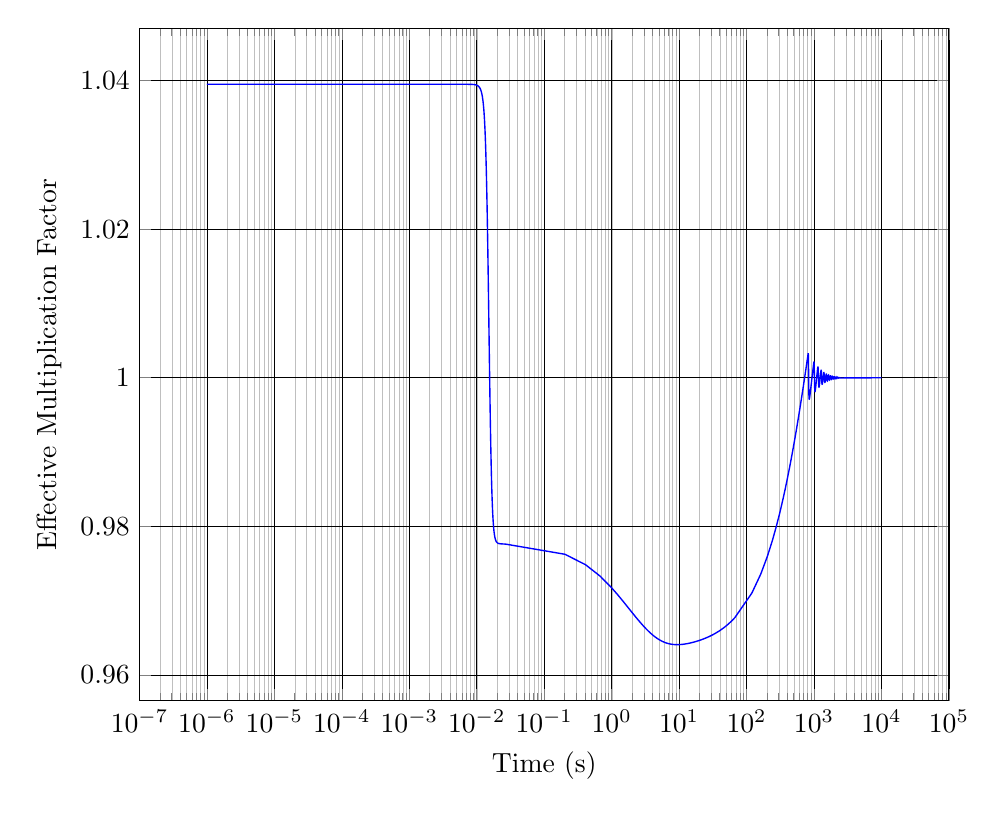
\begin{tikzpicture} \begin{semilogxaxis}
[scale=1.5,
 grid=both, 
 major grid style={color=black,line width=0.2pt},
 minor grid style={color=gray!50,line width=0.1pt},
 xlabel=Time (s),
 ylabel=Effective Multiplication Factor
]

\addplot[color=blue, line width=0.5pt] coordinates {
 ( 1.0e-6,   1.0395 ) 
 ( 2.5e-06 , 1.0395 )
 ( 5e-06 , 1.0395 )
 ( 7.5e-06 , 1.0395 )
 ( 1e-05 , 1.0395 )
 ( 1.25e-05 , 1.0395 )
 ( 1.5e-05 , 1.0395 )
 ( 1.75e-05 , 1.0395 )
 ( 2e-05 , 1.0395 )
 ( 2.25e-05 , 1.0395 )
 ( 2.5e-05 , 1.0395 )
 ( 2.75e-05 , 1.0395 )
 ( 3.25e-05 , 1.0395 )
 ( 3.75e-05 , 1.0395 )
 ( 4.25e-05 , 1.0395 )
 ( 4.75e-05 , 1.0395 )
 ( 5.25e-05 , 1.0395 )
 ( 5.7705e-05 , 1.0395 )
 ( 6.34074e-05 , 1.0395 )
 ( 6.96508e-05 , 1.0395 )
 ( 7.64822e-05 , 1.0395 )
 ( 8.39516e-05 , 1.0395 )
 ( 9.21121e-05 , 1.0395 )
 ( 0.00010102 , 1.0395 )
 ( 0.000110736 , 1.0395 )
 ( 0.000121322 , 1.0395 )
 ( 0.000132845 , 1.0395 )
 ( 0.000145372 , 1.0395 )
 ( 0.000158974 , 1.0395 )
 ( 0.000173726 , 1.0395 )
 ( 0.000189702 , 1.0395 )
 ( 0.000206978 , 1.0395 )
 ( 0.00022563 , 1.0395 )
 ( 0.000245735 , 1.0395 )
 ( 0.000267368 , 1.0395 )
 ( 0.000290604 , 1.0395 )
 ( 0.000315511 , 1.0395 )
 ( 0.000342158 , 1.0395 )
 ( 0.000370606 , 1.0395 )
 ( 0.000400911 , 1.0395 )
 ( 0.000433125 , 1.0395 )
 ( 0.000467288 , 1.0395 )
 ( 0.000503434 , 1.0395 )
 ( 0.000541589 , 1.0395 )
 ( 0.000581768 , 1.0395 )
 ( 0.000623977 , 1.0395 )
 ( 0.000668212 , 1.0395 )
 ( 0.000714458 , 1.0395 )
 ( 0.000762693 , 1.0395 )
 ( 0.000812884 , 1.0395 )
 ( 0.000864989 , 1.0395 )
 ( 0.000918961 , 1.0395 )
 ( 0.000974741 , 1.0395 )
 ( 0.00103227 , 1.0395 )
 ( 0.00109148 , 1.0395 )
 ( 0.0011523 , 1.0395 )
 ( 0.00121465 , 1.0395 )
 ( 0.00127847 , 1.0395 )
 ( 0.00134367 , 1.0395 )
 ( 0.00141017 , 1.0395 )
 ( 0.0014779 , 1.0395 )
 ( 0.00154678 , 1.0395 )
 ( 0.00161674 , 1.0395 )
 ( 0.0016877 , 1.0395 )
 ( 0.00175959 , 1.0395 )
 ( 0.00183236 , 1.0395 )
 ( 0.00190592 , 1.0395 )
 ( 0.00198024 , 1.0395 )
 ( 0.00205523 , 1.0395 )
 ( 0.00213086 , 1.0395 )
 ( 0.00220707 , 1.0395 )
 ( 0.00228381 , 1.0395 )
 ( 0.00236104 , 1.0395 )
 ( 0.00243873 , 1.0395 )
 ( 0.00251682 , 1.0395 )
 ( 0.00259528 , 1.0395 )
 ( 0.00267409 , 1.0395 )
 ( 0.00275322 , 1.0395 )
 ( 0.00283262 , 1.0395 )
 ( 0.00291229 , 1.0395 )
 ( 0.00299219 , 1.0395 )
 ( 0.00307231 , 1.0395 )
 ( 0.00315263 , 1.0395 )
 ( 0.00323312 , 1.0395 )
 ( 0.00331378 , 1.0395 )
 ( 0.00339458 , 1.0395 )
 ( 0.00347551 , 1.0395 )
 ( 0.00355657 , 1.0395 )
 ( 0.00363774 , 1.0395 )
 ( 0.003719 , 1.0395 )
 ( 0.00380036 , 1.0395 )
 ( 0.0038818 , 1.0395 )
 ( 0.00396331 , 1.0395 )
 ( 0.00404489 , 1.0395 )
 ( 0.00412653 , 1.0395 )
 ( 0.00420823 , 1.0395 )
 ( 0.00428998 , 1.0395 )
 ( 0.00437177 , 1.0395 )
 ( 0.00445361 , 1.0395 )
 ( 0.00453548 , 1.0395 )
 ( 0.00461738 , 1.0395 )
 ( 0.00469932 , 1.0395 )
 ( 0.00478128 , 1.0395 )
 ( 0.00486327 , 1.0395 )
 ( 0.00494528 , 1.0395 )
 ( 0.00502731 , 1.0395 )
 ( 0.00510936 , 1.0395 )
 ( 0.00519143 , 1.0395 )
 ( 0.00527351 , 1.0395 )
 ( 0.00535561 , 1.0395 )
 ( 0.00543772 , 1.0395 )
 ( 0.00551984 , 1.0395 )
 ( 0.00560197 , 1.0395 )
 ( 0.00568411 , 1.0395 )
 ( 0.00576626 , 1.0395 )
 ( 0.00584841 , 1.0395 )
 ( 0.00593057 , 1.0395 )
 ( 0.00601274 , 1.0395 )
 ( 0.00609492 , 1.0395 )
 ( 0.0061771 , 1.0395 )
 ( 0.00625928 , 1.0395 )
 ( 0.00634147 , 1.0395 )
 ( 0.00642367 , 1.0395 )
 ( 0.00650586 , 1.0395 )
 ( 0.00658806 , 1.0395 )
 ( 0.00667027 , 1.0395 )
 ( 0.00675247 , 1.0395 )
 ( 0.00683468 , 1.0395 )
 ( 0.00691689 , 1.0395 )
 ( 0.00699911 , 1.0395 )
 ( 0.00708132 , 1.0395 )
 ( 0.00716354 , 1.0395 )
 ( 0.00724576 , 1.0395 )
 ( 0.00732798 , 1.0395 )
 ( 0.0074102 , 1.0395 )
 ( 0.00749243 , 1.03949 )
 ( 0.00757465 , 1.03949 )
 ( 0.00765688 , 1.03949 )
 ( 0.00773911 , 1.03949 )
 ( 0.00782134 , 1.03949 )
 ( 0.00790357 , 1.03949 )
 ( 0.00798581 , 1.03949 )
 ( 0.00806805 , 1.03949 )
 ( 0.00815028 , 1.03949 )
 ( 0.00823252 , 1.03949 )
 ( 0.00831477 , 1.03948 )
 ( 0.00839701 , 1.03948 )
 ( 0.00847926 , 1.03948 )
 ( 0.00856151 , 1.03948 )
 ( 0.00864377 , 1.03948 )
 ( 0.00872602 , 1.03947 )
 ( 0.00880828 , 1.03947 )
 ( 0.00889055 , 1.03947 )
 ( 0.00897282 , 1.03946 )
 ( 0.00905509 , 1.03946 )
 ( 0.00913737 , 1.03946 )
 ( 0.00921965 , 1.03945 )
 ( 0.00930195 , 1.03945 )
 ( 0.00938424 , 1.03944 )
 ( 0.00946655 , 1.03943 )
 ( 0.00954886 , 1.03943 )
 ( 0.00963119 , 1.03942 )
 ( 0.00971352 , 1.03941 )
 ( 0.00979586 , 1.0394 )
 ( 0.00987822 , 1.03939 )
 ( 0.00996059 , 1.03938 )
 ( 0.010043 , 1.03936 )
 ( 0.0101254 , 1.03935 )
 ( 0.0102078 , 1.03933 )
 ( 0.0102902 , 1.03932 )
 ( 0.0103727 , 1.0393 )
 ( 0.0104552 , 1.03927 )
 ( 0.0105377 , 1.03925 )
 ( 0.0106203 , 1.03922 )
 ( 0.0107029 , 1.0392 )
 ( 0.0107855 , 1.03916 )
 ( 0.0108681 , 1.03913 )
 ( 0.0109508 , 1.03909 )
 ( 0.0110336 , 1.03905 )
 ( 0.0111164 , 1.039 )
 ( 0.0111993 , 1.03894 )
 ( 0.0112823 , 1.03889 )
 ( 0.0113653 , 1.03882 )
 ( 0.0114484 , 1.03875 )
 ( 0.0115316 , 1.03867 )
 ( 0.0116149 , 1.03858 )
 ( 0.0116983 , 1.03849 )
 ( 0.0117819 , 1.03838 )
 ( 0.0118656 , 1.03826 )
 ( 0.0119494 , 1.03813 )
 ( 0.0120334 , 1.03799 )
 ( 0.0121177 , 1.03783 )
 ( 0.0122021 , 1.03766 )
 ( 0.0122868 , 1.03746 )
 ( 0.0123717 , 1.03725 )
 ( 0.0124569 , 1.03701 )
 ( 0.0125425 , 1.03675 )
 ( 0.0126284 , 1.03646 )
 ( 0.0127147 , 1.03615 )
 ( 0.0128015 , 1.0358 )
 ( 0.0128888 , 1.03541 )
 ( 0.0129767 , 1.03498 )
 ( 0.0130652 , 1.03451 )
 ( 0.0131544 , 1.03399 )
 ( 0.0132444 , 1.03341 )
 ( 0.0133354 , 1.03278 )
 ( 0.0134273 , 1.03208 )
 ( 0.0135204 , 1.0313 )
 ( 0.0136148 , 1.03045 )
 ( 0.0137107 , 1.02951 )
 ( 0.0138083 , 1.02848 )
 ( 0.0139079 , 1.02734 )
 ( 0.0140096 , 1.02609 )
 ( 0.014114 , 1.02471 )
 ( 0.0142214 , 1.02319 )
 ( 0.0143324 , 1.02152 )
 ( 0.0144475 , 1.01968 )
 ( 0.0145676 , 1.01767 )
 ( 0.0146938 , 1.01545 )
 ( 0.0148273 , 1.01303 )
 ( 0.0149701 , 1.01038 )
 ( 0.0151246 , 1.00748 )
 ( 0.0152944 , 1.00432 )
 ( 0.015485 , 1.00088 )
 ( 0.0157049 , 0.997154 )
 ( 0.0159259 , 0.993761 )
 ( 0.0161754 , 0.990421 )
 ( 0.0163828 , 0.988059 )
 ( 0.0165675 , 0.986261 )
 ( 0.0167379 , 0.984842 )
 ( 0.0168984 , 0.983696 )
 ( 0.0170516 , 0.982757 )
 ( 0.0171994 , 0.981981 )
 ( 0.0173429 , 0.981333 )
 ( 0.017483 , 0.980789 )
 ( 0.0176205 , 0.980331 )
 ( 0.0177558 , 0.979943 )
 ( 0.0178893 , 0.979614 )
 ( 0.0180214 , 0.979335 )
 ( 0.0181522 , 0.979096 )
 ( 0.0182821 , 0.978893 )
 ( 0.0184113 , 0.978719 )
 ( 0.0185397 , 0.97857 )
 ( 0.0186677 , 0.978442 )
 ( 0.0187953 , 0.978332 )
 ( 0.0189227 , 0.978238 )
 ( 0.0190499 , 0.978157 )
 ( 0.019177 , 0.978088 )
 ( 0.0193041 , 0.978028 )
 ( 0.0194313 , 0.977977 )
 ( 0.0195588 , 0.977932 )
 ( 0.0196865 , 0.977894 )
 ( 0.0198147 , 0.977861 )
 ( 0.0199434 , 0.977832 )
 ( 0.0200728 , 0.977807 )
 ( 0.020203 , 0.977786 )
 ( 0.0203343 , 0.977767 )
 ( 0.0204667 , 0.977751 )
 ( 0.0206007 , 0.977737 )
 ( 0.0207364 , 0.977725 )
 ( 0.0208743 , 0.977714 )
 ( 0.0210148 , 0.977705 )
 ( 0.0211585 , 0.977696 )
 ( 0.021306 , 0.977689 )
 ( 0.0214584 , 0.977683 )
 ( 0.0216167 , 0.977677 )
 ( 0.0217825 , 0.977672 )
 ( 0.021958 , 0.977667 )
 ( 0.0221463 , 0.977662 )
 ( 0.0223519 , 0.977658 )
 ( 0.0225819 , 0.977654 )
 ( 0.0228484 , 0.97765 )
 ( 0.0231746 , 0.977646 )
 ( 0.0236127 , 0.977641 )
 ( 0.0243294 , 0.977634 )
 ( 0.0267446 , 0.977613 )
 ( 0.202966 , 0.976245 )
 ( 0.410704 , 0.974834 )
 ( 0.674763 , 0.9733 )
 ( 0.953514 , 0.971936 )
 ( 1.23378 , 0.970779 )
 ( 1.5155 , 0.969792 )
 ( 1.79858 , 0.968948 )
 ( 2.08293 , 0.968225 )
 ( 2.36843 , 0.967605 )
 ( 2.65497 , 0.967072 )
 ( 2.94247 , 0.966615 )
 ( 3.23083 , 0.966222 )
 ( 3.51998 , 0.965884 )
 ( 3.80984 , 0.965594 )
 ( 4.10034 , 0.965345 )
 ( 4.39142 , 0.965132 )
 ( 4.68303 , 0.964951 )
 ( 4.97513 , 0.964795 )
 ( 5.26766 , 0.964663 )
 ( 5.5606 , 0.964551 )
 ( 5.8539 , 0.964457 )
 ( 6.14754 , 0.964377 )
 ( 6.44149 , 0.964311 )
 ( 6.73572 , 0.964256 )
 ( 7.03022 , 0.964211 )
 ( 7.32496 , 0.964175 )
 ( 7.61993 , 0.964146 )
 ( 7.91511 , 0.964123 )
 ( 8.21048 , 0.964106 )
 ( 8.50603 , 0.964094 )
 ( 8.80176 , 0.964086 )
 ( 9.09765 , 0.964082 )
 ( 9.39369 , 0.964081 )
 ( 9.68987 , 0.964082 )
 ( 9.98619 , 0.964087 )
 ( 10.2826 , 0.964093 )
 ( 10.5792 , 0.964101 )
 ( 10.8759 , 0.96411 )
 ( 11.1727 , 0.964121 )
 ( 11.4696 , 0.964133 )
 ( 11.7666 , 0.964147 )
 ( 12.0638 , 0.964161 )
 ( 12.361 , 0.964175 )
 ( 12.6583 , 0.964191 )
 ( 12.9557 , 0.964207 )
 ( 13.2532 , 0.964224 )
 ( 13.5508 , 0.964241 )
 ( 13.8484 , 0.964258 )
 ( 14.1462 , 0.964276 )
 ( 14.444 , 0.964294 )
 ( 14.7419 , 0.964312 )
 ( 15.0399 , 0.96433 )
 ( 15.338 , 0.964349 )
 ( 15.6361 , 0.964368 )
 ( 15.9343 , 0.964387 )
 ( 16.2326 , 0.964406 )
 ( 16.531 , 0.964425 )
 ( 16.8294 , 0.964444 )
 ( 17.1279 , 0.964464 )
 ( 17.4265 , 0.964483 )
 ( 17.7251 , 0.964503 )
 ( 18.0238 , 0.964522 )
 ( 18.3226 , 0.964542 )
 ( 18.6215 , 0.964562 )
 ( 18.9204 , 0.964581 )
 ( 19.2194 , 0.964601 )
 ( 19.5185 , 0.964621 )
 ( 19.8176 , 0.96464 )
 ( 20.1168 , 0.96466 )
 ( 20.4161 , 0.96468 )
 ( 20.7154 , 0.9647 )
 ( 21.0148 , 0.96472 )
 ( 21.3143 , 0.964739 )
 ( 21.6138 , 0.964759 )
 ( 21.9134 , 0.964779 )
 ( 22.2131 , 0.964799 )
 ( 22.5128 , 0.964819 )
 ( 22.8126 , 0.964839 )
 ( 23.1125 , 0.964858 )
 ( 23.4124 , 0.964878 )
 ( 23.7124 , 0.964898 )
 ( 24.0125 , 0.964918 )
 ( 24.3126 , 0.964938 )
 ( 24.6128 , 0.964958 )
 ( 24.9131 , 0.964978 )
 ( 25.2134 , 0.964997 )
 ( 25.5138 , 0.965017 )
 ( 25.8142 , 0.965037 )
 ( 26.1148 , 0.965057 )
 ( 26.4153 , 0.965077 )
 ( 26.716 , 0.965097 )
 ( 27.0167 , 0.965117 )
 ( 27.3175 , 0.965137 )
 ( 27.6183 , 0.965156 )
 ( 27.9192 , 0.965176 )
 ( 28.2201 , 0.965196 )
 ( 28.5212 , 0.965216 )
 ( 28.8222 , 0.965236 )
 ( 29.1234 , 0.965256 )
 ( 29.4246 , 0.965276 )
 ( 29.7258 , 0.965295 )
 ( 30.0271 , 0.965315 )
 ( 30.3284 , 0.965335 )
 ( 30.6298 , 0.965355 )
 ( 30.9313 , 0.965375 )
 ( 31.2328 , 0.965395 )
 ( 31.5343 , 0.965415 )
 ( 31.8359 , 0.965434 )
 ( 32.1374 , 0.965454 )
 ( 32.4391 , 0.965474 )
 ( 32.7407 , 0.965494 )
 ( 33.0423 , 0.965514 )
 ( 33.344 , 0.965534 )
 ( 33.6456 , 0.965554 )
 ( 33.9472 , 0.965573 )
 ( 34.2488 , 0.965593 )
 ( 34.5504 , 0.965613 )
 ( 34.8518 , 0.965633 )
 ( 35.1532 , 0.965653 )
 ( 35.4545 , 0.965672 )
 ( 35.7557 , 0.965692 )
 ( 36.0566 , 0.965712 )
 ( 36.3574 , 0.965732 )
 ( 36.658 , 0.965751 )
 ( 36.9582 , 0.965771 )
 ( 37.2581 , 0.965791 )
 ( 37.5577 , 0.96581 )
 ( 37.8567 , 0.96583 )
 ( 38.1553 , 0.965849 )
 ( 38.4532 , 0.965869 )
 ( 38.7504 , 0.965888 )
 ( 39.0468 , 0.965908 )
 ( 39.3423 , 0.965927 )
 ( 39.6368 , 0.965946 )
 ( 39.93 , 0.965966 )
 ( 40.2219 , 0.965985 )
 ( 40.5124 , 0.966004 )
 ( 40.8012 , 0.966022 )
 ( 41.0882 , 0.966041 )
 ( 41.3731 , 0.96606 )
 ( 41.6424 , 0.966077 )
 ( 41.8814 , 0.966093 )
 ( 42.1303 , 0.966109 )
 ( 42.3834 , 0.966126 )
 ( 42.6394 , 0.966143 )
 ( 42.872 , 0.966158 )
 ( 43.1174 , 0.966174 )
 ( 43.3491 , 0.966189 )
 ( 43.5901 , 0.966205 )
 ( 43.8124 , 0.966219 )
 ( 44.0431 , 0.966234 )
 ( 44.2788 , 0.966249 )
 ( 44.5162 , 0.966265 )
 ( 44.7528 , 0.96628 )
 ( 44.9866 , 0.966296 )
 ( 45.2164 , 0.96631 )
 ( 45.441 , 0.966325 )
 ( 45.6729 , 0.96634 )
 ( 45.8963 , 0.966355 )
 ( 46.1222 , 0.966369 )
 ( 46.3481 , 0.966384 )
 ( 46.5718 , 0.966399 )
 ( 46.8001 , 0.966414 )
 ( 47.0297 , 0.966428 )
 ( 47.2581 , 0.966443 )
 ( 47.4836 , 0.966458 )
 ( 47.7102 , 0.966473 )
 ( 47.9356 , 0.966487 )
 ( 48.1624 , 0.966502 )
 ( 48.3882 , 0.966517 )
 ( 48.6112 , 0.966531 )
 ( 48.8366 , 0.966546 )
 ( 49.0618 , 0.96656 )
 ( 49.2873 , 0.966575 )
 ( 49.5111 , 0.96659 )
 ( 49.7359 , 0.966604 )
 ( 49.9594 , 0.966619 )
 ( 50.1835 , 0.966633 )
 ( 50.4076 , 0.966648 )
 ( 50.6313 , 0.966662 )
 ( 50.8551 , 0.966677 )
 ( 51.0796 , 0.966691 )
 ( 51.3046 , 0.966706 )
 ( 51.5291 , 0.96672 )
 ( 51.7539 , 0.966735 )
 ( 51.9785 , 0.96675 )
 ( 52.204 , 0.966764 )
 ( 52.4295 , 0.966779 )
 ( 52.655 , 0.966793 )
 ( 52.8807 , 0.966808 )
 ( 53.1068 , 0.966823 )
 ( 53.3334 , 0.966837 )
 ( 53.5604 , 0.966852 )
 ( 53.7878 , 0.966867 )
 ( 54.0157 , 0.966881 )
 ( 54.2443 , 0.966896 )
 ( 54.4734 , 0.966911 )
 ( 54.7031 , 0.966926 )
 ( 54.9336 , 0.966941 )
 ( 55.165 , 0.966956 )
 ( 55.3975 , 0.966971 )
 ( 55.6311 , 0.966986 )
 ( 55.8658 , 0.967001 )
 ( 56.1021 , 0.967016 )
 ( 56.3399 , 0.967031 )
 ( 56.5794 , 0.967047 )
 ( 56.8209 , 0.967062 )
 ( 57.0647 , 0.967078 )
 ( 57.3111 , 0.967094 )
 ( 57.5603 , 0.96711 )
 ( 57.813 , 0.967126 )
 ( 58.0693 , 0.967143 )
 ( 58.33 , 0.96716 )
 ( 58.5958 , 0.967177 )
 ( 58.8673 , 0.967194 )
 ( 59.1455 , 0.967212 )
 ( 59.4317 , 0.967231 )
 ( 59.7271 , 0.96725 )
 ( 60.0337 , 0.967269 )
 ( 60.3536 , 0.96729 )
 ( 60.6898 , 0.967312 )
 ( 61.0462 , 0.967334 )
 ( 61.4281 , 0.967359 )
 ( 61.8431 , 0.967386 )
 ( 62.3022 , 0.967415 )
 ( 62.8232 , 0.967449 )
 ( 63.4364 , 0.967488 )
 ( 64.2006 , 0.967537 )
 ( 65.2575 , 0.967605 )
 ( 67.1495 , 0.967726 )
 ( 119.948 , 0.971029 )
 ( 162.656 , 0.973597 )
 ( 203.061 , 0.975944 )
 ( 241.207 , 0.978088 )
 ( 277.142 , 0.980045 )
 ( 310.926 , 0.981831 )
 ( 342.624 , 0.983461 )
 ( 372.309 , 0.984949 )
 ( 400.057 , 0.986305 )
 ( 425.951 , 0.987542 )
 ( 450.074 , 0.988669 )
 ( 472.512 , 0.989698 )
 ( 493.353 , 0.990635 )
 ( 512.686 , 0.991489 )
 ( 530.597 , 0.992268 )
 ( 547.172 , 0.992978 )
 ( 562.497 , 0.993625 )
 ( 576.653 , 0.994216 )
 ( 589.72 , 0.994754 )
 ( 601.775 , 0.995246 )
 ( 612.891 , 0.995694 )
 ( 623.138 , 0.996104 )
 ( 632.582 , 0.996478 )
 ( 641.287 , 0.99682 )
 ( 649.31 , 0.997133 )
 ( 656.708 , 0.99742 )
 ( 663.533 , 0.997683 )
 ( 669.833 , 0.997924 )
 ( 675.653 , 0.998146 )
 ( 681.033 , 0.99835 )
 ( 686.014 , 0.998538 )
 ( 690.629 , 0.998711 )
 ( 694.913 , 0.998872 )
 ( 698.893 , 0.99902 )
 ( 702.598 , 0.999158 )
 ( 706.051 , 0.999286 )
 ( 709.277 , 0.999405 )
 ( 712.295 , 0.999516 )
 ( 715.123 , 0.99962 )
 ( 717.777 , 0.999717 )
 ( 720.275 , 0.999809 )
 ( 722.63 , 0.999895 )
 ( 724.854 , 0.999976 )
 ( 726.956 , 1.00005 )
 ( 728.949 , 1.00012 )
 ( 730.839 , 1.00019 )
 ( 732.636 , 1.00026 )
 ( 734.35 , 1.00032 )
 ( 735.983 , 1.00038 )
 ( 737.546 , 1.00043 )
 ( 739.04 , 1.00049 )
 ( 740.472 , 1.00054 )
 ( 741.849 , 1.00059 )
 ( 743.171 , 1.00064 )
 ( 744.446 , 1.00068 )
 ( 745.677 , 1.00073 )
 ( 746.864 , 1.00077 )
 ( 748.006 , 1.00081 )
 ( 749.111 , 1.00085 )
 ( 750.184 , 1.00089 )
 ( 751.23 , 1.00092 )
 ( 752.248 , 1.00096 )
 ( 753.236 , 1.001 )
 ( 754.194 , 1.00103 )
 ( 755.123 , 1.00106 )
 ( 756.028 , 1.00109 )
 ( 756.916 , 1.00113 )
 ( 757.773 , 1.00116 )
 ( 758.612 , 1.00119 )
 ( 759.45 , 1.00122 )
 ( 760.244 , 1.00124 )
 ( 761.052 , 1.00127 )
 ( 761.824 , 1.0013 )
 ( 762.591 , 1.00133 )
 ( 763.343 , 1.00135 )
 ( 764.066 , 1.00138 )
 ( 764.813 , 1.0014 )
 ( 765.503 , 1.00143 )
 ( 766.196 , 1.00145 )
 ( 766.886 , 1.00148 )
 ( 767.563 , 1.0015 )
 ( 768.21 , 1.00152 )
 ( 768.966 , 1.00155 )
 ( 769.688 , 1.00158 )
 ( 770.336 , 1.0016 )
 ( 771.136 , 1.00163 )
 ( 771.769 , 1.00165 )
 ( 772.392 , 1.00167 )
 ( 773.004 , 1.00169 )
 ( 773.608 , 1.00171 )
 ( 774.202 , 1.00173 )
 ( 774.787 , 1.00175 )
 ( 775.364 , 1.00177 )
 ( 775.932 , 1.00179 )
 ( 776.493 , 1.00181 )
 ( 777.046 , 1.00183 )
 ( 777.591 , 1.00185 )
 ( 778.13 , 1.00187 )
 ( 778.661 , 1.00189 )
 ( 779.186 , 1.00191 )
 ( 779.704 , 1.00192 )
 ( 780.216 , 1.00194 )
 ( 780.721 , 1.00196 )
 ( 781.221 , 1.00198 )
 ( 781.715 , 1.00199 )
 ( 782.203 , 1.00201 )
 ( 782.686 , 1.00203 )
 ( 783.163 , 1.00204 )
 ( 783.635 , 1.00206 )
 ( 784.103 , 1.00208 )
 ( 784.565 , 1.00209 )
 ( 785.022 , 1.00211 )
 ( 785.475 , 1.00212 )
 ( 785.924 , 1.00214 )
 ( 786.367 , 1.00215 )
 ( 786.807 , 1.00217 )
 ( 787.242 , 1.00218 )
 ( 787.673 , 1.0022 )
 ( 788.1 , 1.00221 )
 ( 788.523 , 1.00223 )
 ( 788.943 , 1.00224 )
 ( 789.358 , 1.00226 )
 ( 789.77 , 1.00227 )
 ( 790.178 , 1.00229 )
 ( 790.583 , 1.0023 )
 ( 790.982 , 1.00231 )
 ( 791.378 , 1.00233 )
 ( 791.77 , 1.00234 )
 ( 792.157 , 1.00235 )
 ( 792.541 , 1.00237 )
 ( 792.922 , 1.00238 )
 ( 793.299 , 1.00239 )
 ( 793.672 , 1.0024 )
 ( 794.043 , 1.00242 )
 ( 794.41 , 1.00243 )
 ( 794.775 , 1.00244 )
 ( 795.136 , 1.00245 )
 ( 795.495 , 1.00247 )
 ( 795.85 , 1.00248 )
 ( 796.203 , 1.00249 )
 ( 796.554 , 1.0025 )
 ( 796.902 , 1.00252 )
 ( 797.247 , 1.00253 )
 ( 797.59 , 1.00254 )
 ( 797.93 , 1.00255 )
 ( 798.269 , 1.00256 )
 ( 798.604 , 1.00257 )
 ( 798.938 , 1.00258 )
 ( 799.269 , 1.0026 )
 ( 799.598 , 1.00261 )
 ( 799.925 , 1.00262 )
 ( 800.25 , 1.00263 )
 ( 800.573 , 1.00264 )
 ( 800.893 , 1.00265 )
 ( 801.212 , 1.00266 )
 ( 801.529 , 1.00267 )
 ( 801.844 , 1.00268 )
 ( 802.157 , 1.00269 )
 ( 802.468 , 1.0027 )
 ( 802.777 , 1.00272 )
 ( 803.084 , 1.00273 )
 ( 803.39 , 1.00274 )
 ( 803.693 , 1.00275 )
 ( 803.995 , 1.00276 )
 ( 804.296 , 1.00277 )
 ( 804.594 , 1.00278 )
 ( 804.891 , 1.00279 )
 ( 805.186 , 1.0028 )
 ( 805.48 , 1.00281 )
 ( 805.772 , 1.00282 )
 ( 806.063 , 1.00283 )
 ( 806.351 , 1.00284 )
 ( 806.639 , 1.00285 )
 ( 806.925 , 1.00286 )
 ( 807.209 , 1.00286 )
 ( 807.492 , 1.00287 )
 ( 807.773 , 1.00288 )
 ( 808.053 , 1.00289 )
 ( 808.332 , 1.0029 )
 ( 808.609 , 1.00291 )
 ( 808.884 , 1.00292 )
 ( 809.159 , 1.00293 )
 ( 809.432 , 1.00294 )
 ( 809.703 , 1.00295 )
 ( 809.973 , 1.00296 )
 ( 810.242 , 1.00297 )
 ( 810.51 , 1.00298 )
 ( 810.777 , 1.00298 )
 ( 811.042 , 1.00299 )
 ( 811.306 , 1.003 )
 ( 811.569 , 1.00301 )
 ( 811.83 , 1.00302 )
 ( 812.09 , 1.00303 )
 ( 812.35 , 1.00304 )
 ( 812.608 , 1.00304 )
 ( 812.865 , 1.00305 )
 ( 813.121 , 1.00306 )
 ( 813.375 , 1.00307 )
 ( 813.629 , 1.00308 )
 ( 813.882 , 1.00308 )
 ( 814.133 , 1.00309 )
 ( 814.384 , 1.0031 )
 ( 814.633 , 1.00311 )
 ( 814.882 , 1.00311 )
 ( 815.13 , 1.00312 )
 ( 815.377 , 1.00313 )
 ( 815.623 , 1.00314 )
 ( 815.868 , 1.00314 )
 ( 816.112 , 1.00315 )
 ( 816.356 , 1.00316 )
 ( 816.598 , 1.00316 )
 ( 816.84 , 1.00317 )
 ( 817.082 , 1.00317 )
 ( 817.322 , 1.00318 )
 ( 817.562 , 1.00319 )
 ( 817.802 , 1.00319 )
 ( 818.041 , 1.0032 )
 ( 818.28 , 1.0032 )
 ( 818.518 , 1.0032 )
 ( 818.756 , 1.00321 )
 ( 818.994 , 1.00321 )
 ( 819.231 , 1.00321 )
 ( 819.469 , 1.00322 )
 ( 819.706 , 1.00322 )
 ( 819.944 , 1.00322 )
 ( 820.182 , 1.00322 )
 ( 820.42 , 1.00322 )
 ( 820.659 , 1.00322 )
 ( 820.897 , 1.00321 )
 ( 821.136 , 1.00321 )
 ( 821.376 , 1.00321 )
 ( 821.616 , 1.0032 )
 ( 821.857 , 1.00319 )
 ( 822.099 , 1.00318 )
 ( 822.342 , 1.00317 )
 ( 822.587 , 1.00316 )
 ( 822.833 , 1.00314 )
 ( 823.082 , 1.00312 )
 ( 823.333 , 1.0031 )
 ( 823.588 , 1.00308 )
 ( 823.845 , 1.00305 )
 ( 824.107 , 1.00302 )
 ( 824.373 , 1.00298 )
 ( 824.645 , 1.00294 )
 ( 824.923 , 1.0029 )
 ( 825.209 , 1.00284 )
 ( 825.504 , 1.00278 )
 ( 825.81 , 1.00271 )
 ( 826.129 , 1.00263 )
 ( 826.463 , 1.00254 )
 ( 826.817 , 1.00243 )
 ( 827.195 , 1.0023 )
 ( 827.604 , 1.00216 )
 ( 828.056 , 1.00198 )
 ( 828.566 , 1.00177 )
 ( 829.514 , 1.00135 )
 ( 831.003 , 1.00066 )
 ( 833.734 , 0.999453 )
 ( 835.288 , 0.998882 )
 ( 836.564 , 0.998489 )
 ( 837.717 , 0.998191 )
 ( 838.799 , 0.997956 )
 ( 839.836 , 0.997769 )
 ( 840.842 , 0.997619 )
 ( 841.826 , 0.997498 )
 ( 842.794 , 0.9974 )
 ( 843.751 , 0.997323 )
 ( 844.7 , 0.997262 )
 ( 845.645 , 0.997215 )
 ( 846.585 , 0.99718 )
 ( 847.526 , 0.997154 )
 ( 848.465 , 0.997138 )
 ( 849.407 , 0.997129 )
 ( 850.35 , 0.997126 )
 ( 851.295 , 0.997129 )
 ( 852.242 , 0.997136 )
 ( 853.191 , 0.997148 )
 ( 854.142 , 0.997163 )
 ( 855.098 , 0.997181 )
 ( 856.059 , 0.997202 )
 ( 857.024 , 0.997225 )
 ( 857.997 , 0.99725 )
 ( 858.975 , 0.997278 )
 ( 859.962 , 0.997307 )
 ( 860.956 , 0.997337 )
 ( 861.959 , 0.997369 )
 ( 862.97 , 0.997402 )
 ( 863.992 , 0.997436 )
 ( 865.024 , 0.997471 )
 ( 866.067 , 0.997507 )
 ( 867.121 , 0.997544 )
 ( 868.188 , 0.997582 )
 ( 869.267 , 0.997621 )
 ( 870.36 , 0.99766 )
 ( 871.467 , 0.997701 )
 ( 872.59 , 0.997742 )
 ( 873.728 , 0.997784 )
 ( 874.884 , 0.997827 )
 ( 876.057 , 0.99787 )
 ( 877.249 , 0.997915 )
 ( 878.462 , 0.99796 )
 ( 879.696 , 0.998006 )
 ( 880.953 , 0.998054 )
 ( 882.235 , 0.998102 )
 ( 883.543 , 0.998151 )
 ( 884.879 , 0.998201 )
 ( 886.246 , 0.998252 )
 ( 887.646 , 0.998305 )
 ( 889.083 , 0.998359 )
 ( 890.559 , 0.998415 )
 ( 892.078 , 0.998472 )
 ( 893.646 , 0.99853 )
 ( 895.268 , 0.998591 )
 ( 896.95 , 0.998654 )
 ( 898.701 , 0.99872 )
 ( 900.53 , 0.998788 )
 ( 902.452 , 0.99886 )
 ( 904.483 , 0.998936 )
 ( 906.646 , 0.999016 )
 ( 908.968 , 0.999102 )
 ( 911.498 , 0.999196 )
 ( 914.287 , 0.999299 )
 ( 917.498 , 0.999418 )
 ( 921.304 , 0.999558 )
 ( 926.632 , 0.999753 )
 ( 943.148 , 1.00035 )
 ( 946.018 , 1.00046 )
 ( 948.338 , 1.00054 )
 ( 950.327 , 1.00061 )
 ( 952.094 , 1.00067 )
 ( 953.701 , 1.00073 )
 ( 955.182 , 1.00078 )
 ( 956.563 , 1.00083 )
 ( 957.86 , 1.00088 )
 ( 959.087 , 1.00092 )
 ( 960.254 , 1.00096 )
 ( 961.367 , 1.001 )
 ( 962.434 , 1.00104 )
 ( 963.46 , 1.00108 )
 ( 964.447 , 1.00111 )
 ( 965.402 , 1.00115 )
 ( 966.325 , 1.00118 )
 ( 967.22 , 1.00121 )
 ( 968.089 , 1.00124 )
 ( 968.933 , 1.00127 )
 ( 969.756 , 1.0013 )
 ( 970.558 , 1.00133 )
 ( 971.34 , 1.00135 )
 ( 972.104 , 1.00138 )
 ( 972.852 , 1.00141 )
 ( 973.583 , 1.00143 )
 ( 974.298 , 1.00146 )
 ( 975 , 1.00148 )
 ( 975.688 , 1.0015 )
 ( 976.363 , 1.00153 )
 ( 977.026 , 1.00155 )
 ( 977.677 , 1.00157 )
 ( 978.317 , 1.00159 )
 ( 978.947 , 1.00162 )
 ( 979.566 , 1.00164 )
 ( 980.176 , 1.00166 )
 ( 980.776 , 1.00168 )
 ( 981.368 , 1.0017 )
 ( 981.951 , 1.00172 )
 ( 982.526 , 1.00174 )
 ( 983.093 , 1.00176 )
 ( 983.652 , 1.00177 )
 ( 984.205 , 1.00179 )
 ( 984.75 , 1.00181 )
 ( 985.289 , 1.00183 )
 ( 985.822 , 1.00184 )
 ( 986.348 , 1.00186 )
 ( 986.869 , 1.00188 )
 ( 987.384 , 1.00189 )
 ( 987.893 , 1.00191 )
 ( 988.398 , 1.00192 )
 ( 988.897 , 1.00194 )
 ( 989.392 , 1.00195 )
 ( 989.882 , 1.00197 )
 ( 990.368 , 1.00198 )
 ( 990.851 , 1.00199 )
 ( 991.329 , 1.00201 )
 ( 991.804 , 1.00202 )
 ( 992.275 , 1.00203 )
 ( 992.743 , 1.00204 )
 ( 993.209 , 1.00205 )
 ( 993.672 , 1.00206 )
 ( 994.132 , 1.00207 )
 ( 994.591 , 1.00208 )
 ( 995.048 , 1.00208 )
 ( 995.504 , 1.00209 )
 ( 995.958 , 1.00209 )
 ( 996.412 , 1.0021 )
 ( 996.866 , 1.0021 )
 ( 997.321 , 1.0021 )
 ( 997.776 , 1.0021 )
 ( 998.231 , 1.0021 )
 ( 998.688 , 1.0021 )
 ( 999.145 , 1.00209 )
 ( 999.604 , 1.00208 )
 ( 1000.07 , 1.00207 )
 ( 1000.53 , 1.00206 )
 ( 1001 , 1.00205 )
 ( 1001.47 , 1.00203 )
 ( 1001.96 , 1.002 )
 ( 1002.44 , 1.00197 )
 ( 1002.94 , 1.00194 )
 ( 1003.45 , 1.0019 )
 ( 1003.98 , 1.00186 )
 ( 1004.52 , 1.0018 )
 ( 1005.09 , 1.00174 )
 ( 1005.68 , 1.00167 )
 ( 1006.31 , 1.00158 )
 ( 1006.98 , 1.00148 )
 ( 1007.72 , 1.00136 )
 ( 1008.55 , 1.00121 )
 ( 1010.07 , 1.0009 )
 ( 1012.55 , 1.00035 )
 ( 1016.87 , 0.999443 )
 ( 1019.04 , 0.999072 )
 ( 1020.82 , 0.998823 )
 ( 1022.4 , 0.998641 )
 ( 1023.89 , 0.998503 )
 ( 1025.31 , 0.998397 )
 ( 1026.69 , 0.998315 )
 ( 1028.04 , 0.998254 )
 ( 1029.38 , 0.998209 )
 ( 1030.7 , 0.998178 )
 ( 1032.02 , 0.998159 )
 ( 1033.33 , 0.998149 )
 ( 1034.66 , 0.998147 )
 ( 1035.98 , 0.998153 )
 ( 1037.31 , 0.998164 )
 ( 1038.64 , 0.998182 )
 ( 1039.99 , 0.998204 )
 ( 1041.36 , 0.99823 )
 ( 1042.74 , 0.99826 )
 ( 1044.14 , 0.998293 )
 ( 1045.56 , 0.99833 )
 ( 1047.01 , 0.99837 )
 ( 1048.49 , 0.998413 )
 ( 1050.01 , 0.998458 )
 ( 1051.56 , 0.998506 )
 ( 1053.16 , 0.998557 )
 ( 1054.8 , 0.99861 )
 ( 1056.5 , 0.998667 )
 ( 1058.26 , 0.998726 )
 ( 1060.1 , 0.998789 )
 ( 1062.02 , 0.998855 )
 ( 1064.04 , 0.998926 )
 ( 1066.18 , 0.999001 )
 ( 1068.47 , 0.999082 )
 ( 1070.94 , 0.999169 )
 ( 1073.65 , 0.999266 )
 ( 1076.71 , 0.999375 )
 ( 1080.26 , 0.999502 )
 ( 1084.87 , 0.999667 )
 ( 1092.4 , 0.999935 )
 ( 1102.85 , 1.0003 )
 ( 1106.03 , 1.00042 )
 ( 1108.53 , 1.0005 )
 ( 1110.65 , 1.00058 )
 ( 1112.52 , 1.00064 )
 ( 1114.21 , 1.0007 )
 ( 1115.77 , 1.00075 )
 ( 1117.21 , 1.0008 )
 ( 1118.57 , 1.00085 )
 ( 1119.85 , 1.00089 )
 ( 1121.07 , 1.00093 )
 ( 1122.23 , 1.00097 )
 ( 1123.35 , 1.001 )
 ( 1124.42 , 1.00104 )
 ( 1125.46 , 1.00107 )
 ( 1126.46 , 1.0011 )
 ( 1127.43 , 1.00113 )
 ( 1128.38 , 1.00116 )
 ( 1129.3 , 1.00119 )
 ( 1130.19 , 1.00121 )
 ( 1131.07 , 1.00124 )
 ( 1131.93 , 1.00126 )
 ( 1132.77 , 1.00128 )
 ( 1133.59 , 1.0013 )
 ( 1134.4 , 1.00132 )
 ( 1135.2 , 1.00134 )
 ( 1135.99 , 1.00136 )
 ( 1136.77 , 1.00137 )
 ( 1137.53 , 1.00139 )
 ( 1138.29 , 1.0014 )
 ( 1139.05 , 1.00141 )
 ( 1139.79 , 1.00142 )
 ( 1140.54 , 1.00143 )
 ( 1141.28 , 1.00144 )
 ( 1142.02 , 1.00144 )
 ( 1142.76 , 1.00144 )
 ( 1143.5 , 1.00144 )
 ( 1144.24 , 1.00144 )
 ( 1144.99 , 1.00143 )
 ( 1145.74 , 1.00142 )
 ( 1146.5 , 1.00141 )
 ( 1147.27 , 1.00139 )
 ( 1148.05 , 1.00137 )
 ( 1148.85 , 1.00134 )
 ( 1149.67 , 1.0013 )
 ( 1150.52 , 1.00126 )
 ( 1151.41 , 1.0012 )
 ( 1152.35 , 1.00114 )
 ( 1153.35 , 1.00106 )
 ( 1154.44 , 1.00097 )
 ( 1155.68 , 1.00085 )
 ( 1158 , 1.00059 )
 ( 1162.42 , 1.00005 )
 ( 1166.39 , 0.999596 )
 ( 1168.58 , 0.999379 )
 ( 1171.14 , 0.999169 )
 ( 1173.35 , 0.999025 )
 ( 1175.38 , 0.998923 )
 ( 1177.31 , 0.99885 )
 ( 1179.17 , 0.998799 )
 ( 1181.02 , 0.998765 )
 ( 1182.83 , 0.998746 )
 ( 1184.65 , 0.998739 )
 ( 1186.46 , 0.998743 )
 ( 1188.29 , 0.998755 )
 ( 1190.14 , 0.998775 )
 ( 1192.02 , 0.998803 )
 ( 1193.95 , 0.998837 )
 ( 1195.93 , 0.998877 )
 ( 1197.97 , 0.998923 )
 ( 1200.09 , 0.998975 )
 ( 1202.31 , 0.999033 )
 ( 1204.66 , 0.999098 )
 ( 1207.17 , 0.99917 )
 ( 1209.89 , 0.999251 )
 ( 1212.9 , 0.999344 )
 ( 1216.35 , 0.999451 )
 ( 1220.51 , 0.999584 )
 ( 1226.32 , 0.999772 )
 ( 1244.16 , 1.00034 )
 ( 1247.15 , 1.00044 )
 ( 1249.59 , 1.00051 )
 ( 1251.72 , 1.00057 )
 ( 1253.63 , 1.00063 )
 ( 1255.38 , 1.00068 )
 ( 1257.01 , 1.00072 )
 ( 1258.54 , 1.00076 )
 ( 1260 , 1.0008 )
 ( 1261.39 , 1.00083 )
 ( 1262.72 , 1.00086 )
 ( 1264.01 , 1.00089 )
 ( 1265.26 , 1.00091 )
 ( 1266.48 , 1.00094 )
 ( 1267.68 , 1.00096 )
 ( 1268.85 , 1.00097 )
 ( 1270 , 1.00099 )
 ( 1271.14 , 1.001 )
 ( 1272.28 , 1.001 )
 ( 1273.41 , 1.00101 )
 ( 1274.54 , 1.00101 )
 ( 1275.68 , 1.001 )
 ( 1276.82 , 1.001 )
 ( 1277.98 , 1.00098 )
 ( 1279.16 , 1.00096 )
 ( 1280.37 , 1.00094 )
 ( 1281.62 , 1.0009 )
 ( 1282.92 , 1.00086 )
 ( 1284.32 , 1.0008 )
 ( 1285.83 , 1.00073 )
 ( 1287.52 , 1.00064 )
 ( 1290.73 , 1.00043 )
 ( 1297.5 , 0.999939 )
 ( 1302.69 , 0.999597 )
 ( 1306.42 , 0.999405 )
 ( 1309.45 , 0.999289 )
 ( 1312.2 , 0.999213 )
 ( 1314.8 , 0.999164 )
 ( 1317.33 , 0.999137 )
 ( 1319.85 , 0.999127 )
 ( 1322.37 , 0.999131 )
 ( 1324.91 , 0.999148 )
 ( 1327.52 , 0.999176 )
 ( 1330.21 , 0.999215 )
 ( 1333.04 , 0.999264 )
 ( 1336.05 , 0.999323 )
 ( 1339.34 , 0.999396 )
 ( 1343.03 , 0.999484 )
 ( 1347.41 , 0.999595 )
 ( 1353.27 , 0.999752 )
 ( 1374.42 , 1.00032 )
 ( 1377.72 , 1.0004 )
 ( 1380.45 , 1.00046 )
 ( 1382.85 , 1.00052 )
 ( 1385.04 , 1.00056 )
 ( 1387.07 , 1.0006 )
 ( 1388.99 , 1.00063 )
 ( 1390.82 , 1.00065 )
 ( 1392.58 , 1.00068 )
 ( 1394.3 , 1.00069 )
 ( 1396 , 1.0007 )
 ( 1397.67 , 1.00071 )
 ( 1399.35 , 1.00071 )
 ( 1401.03 , 1.00071 )
 ( 1402.74 , 1.00069 )
 ( 1404.48 , 1.00067 )
 ( 1406.29 , 1.00064 )
 ( 1408.2 , 1.0006 )
 ( 1410.26 , 1.00055 )
 ( 1412.58 , 1.00047 )
 ( 1417.09 , 1.00029 )
 ( 1432.59 , 0.999638 )
 ( 1437.08 , 0.999508 )
 ( 1440.9 , 0.999434 )
 ( 1444.42 , 0.999395 )
 ( 1447.86 , 0.999379 )
 ( 1451.27 , 0.999383 )
 ( 1454.76 , 0.999405 )
 ( 1458.4 , 0.999442 )
 ( 1462.31 , 0.999496 )
 ( 1466.68 , 0.999569 )
 ( 1471.9 , 0.999669 )
 ( 1479.2 , 0.999823 )
 ( 1498.77 , 1.00025 )
 ( 1503.02 , 1.00033 )
 ( 1506.42 , 1.00038 )
 ( 1509.4 , 1.00043 )
 ( 1512.12 , 1.00046 )
 ( 1514.68 , 1.00048 )
 ( 1517.13 , 1.0005 )
 ( 1519.53 , 1.00051 )
 ( 1521.91 , 1.00051 )
 ( 1524.31 , 1.0005 )
 ( 1526.78 , 1.00049 )
 ( 1529.35 , 1.00046 )
 ( 1532.13 , 1.00041 )
 ( 1535.27 , 1.00035 )
 ( 1541.75 , 1.00017 )
 ( 1557.99 , 0.999722 )
 ( 1563.95 , 0.999618 )
 ( 1568.89 , 0.999572 )
 ( 1573.63 , 0.999558 )
 ( 1578.32 , 0.99957 )
 ( 1583.27 , 0.999605 )
 ( 1588.78 , 0.999666 )
 ( 1595.56 , 0.999762 )
 ( 1606.93 , 0.999952 )
 ( 1622.02 , 1.0002 )
 ( 1627.34 , 1.00027 )
 ( 1631.57 , 1.00031 )
 ( 1635.31 , 1.00034 )
 ( 1638.8 , 1.00036 )
 ( 1642.18 , 1.00037 )
 ( 1645.57 , 1.00036 )
 ( 1649.09 , 1.00034 )
 ( 1652.89 , 1.0003 )
 ( 1659.93 , 1.0002 )
 ( 1684.63 , 0.999752 )
 ( 1691.86 , 0.999696 )
 ( 1698.34 , 0.999687 )
 ( 1705.01 , 0.999712 )
 ( 1712.59 , 0.999773 )
 ( 1723.35 , 0.999897 )
 ( 1745.47 , 1.00017 )
 ( 1751.94 , 1.00022 )
 ( 1757.23 , 1.00025 )
 ( 1762.09 , 1.00026 )
 ( 1766.9 , 1.00026 )
 ( 1771.99 , 1.00023 )
 ( 1781.54 , 1.00013 )
 ( 1807.58 , 0.999817 )
 ( 1817.17 , 0.999777 )
 ( 1826.28 , 0.999792 )
 ( 1836.93 , 0.999857 )
 ( 1876.47 , 1.00018 )
 ( 1883.38 , 1.00019 )
 ( 1890.2 , 1.00017 )
 ( 1902.92 , 1.00009 )
 ( 1933.05 , 0.999854 )
 ( 1945.63 , 0.999845 )
 ( 1960.08 , 0.999907 )
 ( 1999.28 , 1.00013 )
 ( 2008.75 , 1.00013 )
 ( 2026.11 , 1.00005 )
 ( 2060.43 , 0.999887 )
 ( 2078.27 , 0.999919 )
 ( 2130.04 , 1.00009 )
 ( 2154.88 , 1.00001 )
 ( 2183.14 , 0.999919 )
 ( 2209.44 , 0.999971 )
 ( 2248.43 , 1.00007 )
 ( 2277.9 , 1 )
 ( 2317.9 , 0.999949 )
 ( 2397.9 , 1.00001 )
 ( 2447.9 , 0.999973 )
 ( 10000,   1 )
};
\end{semilogxaxis}
\end{tikzpicture}
\caption{Effective multiplication factor for fission reactor kinetics example.}
 \label{Fig:ode_effectiveMultiplication}
\end{center}
\end{figure}

Since the system is immediately prompt supercritical $(\rho > \beta; \alpha > 0)$ we can expect the fission density to rise exponentially at a rapid pace on the time scale of milliseconds, since the neutron lifetime is 25 microseconds. Eventually, we observe that the fission rate density rapidly experiences a decrease, which is a result of the temperature feedback with negative $\kappa$. As the temperature increases for the fission energy release, the reactivity deceases until the system becomes subcritical and the fission rate rapidly drops.

However, during the prompt transient there was a significant buildup of fission product precursors. These do not simply disappear when the reactor goes subcritical. Rather, there is an exponentially decaying source of neutrons that is driving the subcritical reactor and producing more fission. Since the half-life of these fission products is on the order of a second, the time scale for this source term is on the order of a few tens of seconds. During this time, the reactor continues to heat up as the resulting fissions release more energy.

Finally after most of the precursors have decayed away, the reactor begins to cool steadily, which causes the reactivity to increase again. The cooling process is on the order of minutes. After several minutes, the reactor becomes critical again and another, but less severe, transient will occur. This transient is in the delayed supercritical regime, which means the power rise is on the order of tens of seconds. Eventually the temperature increases, driving the reactor subcritical, leading to the power to fall rapidly with the decay of fission products. The process repeats again and again in a damped oscillation until an equilibrium power is reached.


\clearpage
%%%%%%%%%%%%%%%%%%%%%%%%%%%%%%%%%%%%%%%%%%%%%%%%%%%%%%%%%%%%%%%%%%%%%%%%%%%%%%%%%%%%%%%%%%%%%%%%
%%%%%%%%%%%%%%%%%%%%%%%%%%%%%%%%%%%%%%%%%%%%%%%%%%%%%%%%%%%%%%%%%%%%%%%%%%%%%%%%%%%%%%%%%%%%%%%%
\section{Second-Order Linear ODEs}

Until now, we discussed systems of first-order linear ordinary differential equations. The presence of only the first derivative led to a set of solution techniques involving the integrating factor. Once second-derivatives are added, such techniques no longer apply. 

Additionally, first-order ODEs often describe \emph{initial-value problems} that takes a known value at some point and propagates it forward in whatever variable is involved, usually time. Second-order ODEs can also describe initial-value problems and are often used in the equations of motion for dynamical systems relating position and velocity where both are known at an initial time. It turns out many of the same techniques we used in first-order ODEs are directly applicable for this class of problems.

Another class of problems that are also associated with second-order ODEs are \emph{boundary value problems} that describe the solution of a field (such as temperature) in the interior of an object where some constraints, called boundary conditions, are made on the exterior of the region. This class of problems has fundamentally different properties, and will be the primary focus of the remainder of this chapter.

The second-order linear ODE takes the form:
\begin{align}
  \frac{d^2 y}{dx^2} + p(x) \frac{dy}{dx} + q(x) y(x) = r(x).
\end{align}
When $p(x)$ and $q(x)$ are not constant, it is difficult, if not impossible, to obtain an analytical solution and the equations then need to be solved numerically. Fortunately, many problems of practical interest have constant coefficients, which are amenable to analytical techniques. The simplified version with constant coefficients is written as
\begin{align}
  \frac{d^2 y}{dx^2} + a \frac{dy}{dx} + b y(x) = r(x).
\end{align}

To solve linear second-order ODEs with constant coefficients, we often split the problem into two major steps. First, we solve the homogeneous version by setting the right-hand side equation to zero:
\begin{align}
  \frac{d^2 y_h}{dx^2} + a \frac{dy_h}{dx} + b y_h(x) = 0.
\end{align}
Once we have obtained a solution, we then find another solution called the particular solution 
\begin{align}
  \frac{d^2 y_p}{dx^2} + a \frac{dy_p}{dx} + b y_p(x) = r(x).
\end{align}
These two solutions can be combined to obtain the generation solution to the problem:
\begin{align}
  y(x) = y_h(x) + y_p(x).
\end{align}
These are discussed in the remainder of this section.

%%%%%%%%%%%%%%%%%%%%%%%%%%%%%%%%%%%%%%%%%%%%%%%%%%%%%%%%%%%%%%%%%%%%%%%%%%%%%%%%%%%%%%%%%%%%%%%%
\subsection{Solution of the Homogeneous Problem}

To solve for $y_h(x)$ we make a guess that the solution follows an exponential form:
\begin{align}
  y_h(x) = C e^{\lambda x}
\end{align}
with $C$ as some scaling constant (which we find using boundary conditions) and $\lambda$ some unknown parameter that we hope to find. Inserting this guess into the homogeneous second-order ODE gives:
\begin{align}
  C \lambda^2 e^{\lambda x} + C a \lambda e^{\lambda x} + C b e^{\lambda x} = 0.
\end{align}\
The factor 
\begin{align}
C e^{\lambda x} \nonumber
\end{align}
is common on all terms and, because the right-hand side is zero, they are simply scaling constants and can be divided out. This leaves the quadratic polynomial
\begin{align}
  \lambda^2 + a \lambda + b = 0,
\end{align}
which has the solution via the quadratic formula of
\begin{align}
  \lambda = \frac{1}{2} \left(  -a \pm \sqrt{ a^2 - 4b } \right).
\end{align}
Assuming that the two roots are distinct, call them $\lambda_1$ and $\lambda_2$, we can write the solution to the homogeneous problem as a linear combination of those solutions:
\begin{align}
  y_h(x) = C_1 e^{\lambda_1 x} + C_2 e^{\lambda_2 x}.
\end{align}
When $\lambda_1 = \lambda_2$, we have the case where we need to find another solution. It turns out that when this is the case,
\begin{align}
C x e^{\lambda x} \nonumber
\end{align}
also satisfies the differential equation. Therefore, when $\lambda_1 = \lambda_2 = \lambda$ we can write the solution as
\begin{align}
  y_h(x) = ( C_1 + C_2 x ) e^{\lambda x}.
\end{align}
Note that there are two coefficients $C_1$ and $C_2$, which are the consequence of ``integrating'' twice. These will be solved using the initial or boundary conditions, depending on the class of problem.

When $\lambda$ is real and of the form $\lambda = \pm \mu$, we can express the homogeneous solution in terms of exponentials or hyperbolic trigonometric functions:
\begin{align}
  y_h(x) &= C_1 e^{\mu x} + C_2 e^{-\mu x}, \\ \nonumber
  y_h(x) &= A_1 \sinh (\mu x) + A_2 \cosh ( \mu x ). \nonumber 
\end{align}
Here the constant coefficients are different. The hyperbolic trigonometric functions are related to the exponential by
\begin{subequations}
\begin{align}
  \sinh(x) &= \frac{ e^x - e^{-x} }{ 2 }, \\
  \cosh(x) &= \frac{ e^x + e^{-x} }{ 2 }.
\end{align}
\end{subequations}
The choice of exponentials or hyperbolic trigonometric functions is arbitrary and motivated by whatever makes the math easier. For example, in some boundary value problems, the hyperbolic trigonometric functions can be crafted in a way to eliminate one of the constant coefficients and simplify the form of the solution.

When $\lambda$ is imaginary or complex, we can either work in complex exponentials (often more convenient) or apply Euler's formula to express the solution as trigonometric functions. For purely imaginary $\lambda = \pm i \omega$ functions the homogeneous solution takes either form:
\begin{align}
  y_h(x) &= C_1 e^{i \omega x} + C_2 e^{-i \omega x}, \\ \nonumber
  y_h(x) &= A_1 \sin (\omega x) + A_2 \cos ( \omega x ). \nonumber 
\end{align}
For the more general case of a complex $\lambda = \mu \pm i \omega$, the homogeneous solution may be written as
\begin{align}
  y_h(x) &= A_1 e^{\mu x} \sin (\omega x) + A_2 e^{\mu x} \cos ( \omega x ). \nonumber 
\end{align}

When working with trigonometric or hyperbolic trigonometric functions, it can also be beneficial to apply a \emph{phase shift}. For example, the homogeneous solutions for the real problem with $\lambda = \pm \mu$ could also be written as
\begin{align}
  y_h(x) = B_1 \sinh( \mu x + \varphi )  + B_2 \cosh( \mu x + \varphi ) , \nonumber
\end{align}
and for $\lambda = \pm i \omega$, the homogeneous solution can be written as
\begin{align}
  y_h(x) = B_1 \sin( \omega x + \varphi ) + B_2 \cos( \omega x + \varphi ) . \nonumber
\end{align}

%%%%%%%%%%%%%%%%%%%%%%%%%%%%%%%%%%%%%%%%%%%%%%%%%%%%%%%%%%%%%%%%%%%%%%%%%%%%%%%%%%%%%%%%%%%%%%%%
\subsection{Linear Independence and the Wronskian}

In the previous section, we provided various examples of homogeneous solutions that are possible; however, it would be good to offer a more general set of rules. When we are solving a homogeneous second-order ordinary differential equations, there are two derivatives and we must find two linearly independent functions that satisfy the homogeneous differential equation. Any two will work, so long as they satisfy this criterion.

Assessing linear independence can be done using an object called the \emph{Wronskian}. Suppose we have two solutions $y_1(x)$ and $y_2(x)$ that satisfy the homogeneous differential equation, the Wronskian is given by the following determinant:
\begin{align}
  W(x) = \left| \begin{array}{r r}
  y_1(x)  & y_2(x)   \\
  y_1'(x) & y_2'(x)  \\ \end{array} \right| = y_1(x) y_2'(x) - y_2(x) y_1'(x).
\end{align}
The test for linear independence is
\begin{align}
  W(x) \ne 0 \text{ for some values of $x$ in the domain.}
\end{align}
Conversely, if $y_1(x)$ and $y_2(x)$ satisfy the homogeneous differential equation and $W(x) = 0$ for all $x$ in the domain, then the solutions are linearly dependent and we require a different linearly independent solution.

As an example, consider the homogeneous differential equation:
\begin{subequations}
\begin{align}
  y''(x) + 4 y(x) = 0.
\end{align}
Suppose we wish to determine if
\begin{align}
  y_1(x) &= \sin( 2x ) \\
  y_2(x) &= \sin( 1 - 2x )
\end{align}
are linearly independent solutions. First, we plug in the solutions into the differential equation:
\begin{align}
  -4 \sin( 2x ) + 4 \sin ( 2x ) = 0, \\
  -4 \sin( 1 - 2x ) + 4 \sin ( 1 - 2x ) = 0.
\end{align}
These solutions satisfy the differential equation. The Wronskian is
\begin{align}
  W(x)  &= \left| \begin{array}{r r}
  \sin( 2x )  & \sin( 1 - 2x )   \\
  2 \cos( 2 x) & -2 \cos( 1 - 2x )  \\ \end{array} \right| \nonumber \\ 
  &= -2 \sin( 2x ) \cos( 1 - 2x ) - 2 \cos( 2x ) \sin( 1 - 2x ) = -2 \sin(1).
\end{align}
Since $-2 \sin(1) \ne 0$, then we know both $y_1(x)$ and $y_2(x)$ are linearly independent solutions of the homogeneous differential equation. Therefore, we can write the solution as
\begin{align}
  y(x) = C_1 \sin( 2 x ) + C_2 \sin( 1 - 2x ).
\end{align}
\end{subequations}

Now that the homogeneous solution is known, we must find the particular solution. This is done with one of two approaches: method of undetermined coefficients and variation of parameters.

%%%%%%%%%%%%%%%%%%%%%%%%%%%%%%%%%%%%%%%%%%%%%%%%%%%%%%%%%%%%%%%%%%%%%%%%%%%%%%%%%%%%%%%%%%%%%%%%
\subsection{Method of Undetermined Coefficients}

An approach that is relatively simple, but only works in a narrow set of situations for specific forms of the inhomogeneous term $r(x)$ is called the method of undetermined coefficients. The basic approach is to ``guess'' a functional form for $y_p(x)$ and, should that form be reasonable, we can solve for the coefficients. We now outline a few common cases:

For the case where the inhomogeneous term is a polynomial,
\begin{align}
  r(x) = r_0 + r_1 x + r_2 x^2 + \ldots
\end{align}
we can guess that the particular solution is a polynomial
\begin{align}
  f_h(x) = a_0 + a_1 x + a_2 x^2 + \ldots
\end{align}
plug it into the equation and match the coefficients.

To illustrate, consider the ODE:
\begin{subequations}
\begin{align}
  y''(x) + 4 y'(x) + 3 y(x) = 1 + 3 x^2.
\end{align}
We can guess the particular solution as a quadratic polynomial
\begin{align}
  y_p(x) = a_0 + a_1 x + a_2 x^2.
\end{align}
Inserting this into the differential equation gives
\begin{align}
  2 a_2 + 4 ( 2 a_2 x + a_1 ) + 3 ( a_0 + a_1 x + a_2 x^2 ) = 1 + 0 x^2 + 3 x^2.
\end{align}
Rearranging to combine terms gives
\begin{align}
  ( 3 a_0 + 4 a_1 + 2 a_2 ) + ( 3 a_1 + 8 a_2 ) x + 3 a_2 x^2 = 1 + 0 x^2 + 3 x^2.
\end{align}
By matching coefficients we can determine
\begin{align}
  3 a_0 + 4 a_1 + 2 a_2 &= 1, \nonumber \\
  3 a_1 + 8 a_2 &= 0, \nonumber \\
  3 a_2 &= 3;
\end{align}
or as a linear system
\begin{align}
  \left[ \begin{array}{r r r} 
   3 &  4 &  2 \\
   0 &  3 &  8 \\
   0 &  0 &  3 \\ \end{array} \right]
  \left[ \begin{array}{c} a_0 \\ a_1 \\ a_2 \\ \end{array} \right] =
  \left[ \begin{array}{c} 1 \\ 0 \\ 3 \end{array} \right] .
\end{align}
Solving this linear system gives
\begin{align}
   \left[ \begin{array}{c} a_0 \\ a_1 \\ a_2 \\ \end{array} \right] =
   \left[ \begin{array}{c} \rfrac{29}{9} \\ -\rfrac{8}{3} \\ 1 \\ \end{array} \right]
\end{align}
Therefore, the particular solution is
\begin{align}
  y_p(x) = \frac{29}{9} x^2 - \frac{8}{3} x + 1.
\end{align}
\end{subequations}

Another form is where the inhomogeneous term has the function of an exponential:
\begin{align}
  r(x) = k_0 e^{\beta x}.
\end{align}
For this, we guess a particular solution of the form
\begin{align}
  y_p(x) = a_0 e^{-\beta x}.
\end{align}
More generally, if we have an inhomogeneous solution of the form
\begin{align}
  r(x) = ( k_0 + k_1 x + k_2 x^2 + \ldots ) e^{-\beta x}.
\end{align}
we guess a solution of the form
\begin{align}
  y_p(x) = ( a_0 + a_1 x + a_2 x^2 ) e^{-\beta x}.
\end{align}

Another form for the inhomogeneous term where method of coefficients will work is where the inhomogeneous term is a trigonometric function:
\begin{align}
  r(x) &= k_0 \sin( \alpha x ), \nonumber \\
  r(x) &= k_0 \cos( \alpha x ).
\end{align}
In either of these cases, we guess a particular solution of the form
\begin{align}
  y_p(x) = a_0 \sin( \alpha x ) + b_0 \cos( \alpha x ).
\end{align}
As with the exponential case, these can be generalized to account for polynomial coefficients
\begin{align}
  r(x) = ( k_0 + k_1 x + k_2 x^2 + \ldots ) \sin( \alpha x ), \nonumber \\
  r(x) = ( k_0 + k_1 x + k_2 x^2 + \ldots ) \cos( \alpha x );
\end{align}
we guess a solution of the form
\begin{align}
  y_p(x) = ( a_0 + a_1 x + a_2 x^2 + \ldots ) \sin( \alpha x ) + ( b_0 + b_1 x + b_2 x^2 + \ldots )  \cos( \alpha x ).
\end{align}

If we encounter a linear combination of polynomials, exponentials, and/or trigonometric functions, we can guess that a solution is the linear combination of the guesses with the combined coefficients. As with the polynomial case, the goal is to take the guess, plug it into the differential equation, collect like terms, and solve a linear system for the coefficients. 

To illustrate, consider the example
\begin{subequations}
\begin{align}
  y''(x) + 4 y'(x) + 3 y(x) = 1 + 2 x + 3 x \cos x.
\end{align}
For this we guess a function of five coefficients
\begin{align}
  y_p(x) = a_0 + a_1 x + b_0 \sin x + b_1 x \sin x + c_0 \cos x + c_1 x \cos x.
\end{align}
The derivatives are
\begin{align}
  y_p'(x) &= a_1 + b_0 \cos x + b_1 ( \sin x  + x \cos x ) - c_0 \sin x + c_1 ( \cos x - x \sin x ) \nonumber \\
          &= a_1 + ( b_1 - c_0 ) \sin x  - c_1 x \sin x  + ( b_0 + c_1 ) \cos x + b_1 x \cos x; \\
  y_p''(x) &= ( b_1 - c_0 ) \cos x - c_1 ( \sin x + x \cos x ) - ( b_0 + c_1 ) \sin x + b_1 ( \cos x - x \sin x ) \nonumber \\
           &= -( 2 c_1 + b_0 ) \sin x - b_1 x \sin x + ( 2 b_1 - c_0 ) \cos x - c_1 x \cos x.
\end{align}
Inserting this into the differential equation gives
\begin{align}
  &                -( 2 c_1 + b_0 ) \sin x - b_1 x \sin x + ( 2 b_1 - c_0 ) \cos x - c_1 x \cos x    \nonumber \\
  &4 ( a_1 +          ( b_1 - c_0 ) \sin x - c_1 x \sin x   + ( b_0 + c_1 ) \cos x + b_1 x \cos x )  \nonumber \\
  &3 ( a_0 + a_1 x +            b_0 \sin x + b_1 x \sin x             + c_0 \cos x + c_1 x \cos x )  \nonumber 
  &= 1 + 2 x + 3 x \cos x.
\end{align}
Matching coefficients, this yields a system of equations
\begin{align}  
  3 a_0 + 4 a_1 &= 1, \nonumber \\
  3 a_1 x &= 2x, \nonumber \\
                  ( 2 b_0 + 4 b_1 - 4 c_0 - 2 c_1 )   \sin x &= 0 \sin x, \nonumber \\
                  (         2 b_1         - 4 c_1 ) x \sin x &= 0 x \sin x, \nonumber \\
                  ( 4 b_0 + 2 b_1 + 2 c_0 + 4 c_1 )   \cos x &= 0 \cos x, \nonumber \\      
                  (         4 b_1         + 2 c_1 ) x \cos x &= 3 x \cos x,
\end{align}
which written as a linear system
\begin{align}
  \left[ \begin{array}{r r r r r r} 
   3 &  4 &  0 &  0 &  0 &  0 \\
   0 &  3 &  0 &  0 &  0 &  0 \\
   0 &  0 &  2 &  4 & -4 & -2 \\
   0 &  0 &  0 &  2 &  0 & -4 \\
   0 &  0 &  4 &  2 &  2 &  4 \\
   0 &  0 &  0 &  4 &  0 &  2  
  \end{array} \right]
  \left[ \begin{array}{c} a_0 \\ a_1 \\ b_0 \\ b_1 \\ c_0 \\ c_1 \\\end{array} \right] =
  \left[ \begin{array}{c} 1 \\ 2 \\ 0 \\ 0 \\ 0 \\ 3 \end{array} \right] .
\end{align}
Solving this system yields
\begin{align}
  \left[ \begin{array}{c} a_0 \\ a_1 \\ b_0 \\ b_1 \\ c_0 \\ c_1 \\\end{array} \right] =
  \left[ \begin{array}{c} -\rfrac{5}{9} \\ \rfrac{2}{3} \\ -\rfrac{33}{50} \\ \rfrac{3}{5} \\ \rfrac{3}{25} \\ \rfrac{3}{10} \end{array} \right] .
\end{align}
The particular solution is therefore:
\begin{align}
  y_p(x) = -\frac{5}{9} + \frac{2}{3} x - \frac{33}{50} \sin x + \frac{3}{5} x \sin x + \frac{3}{25} \cos x + \frac{3}{10} x \cos x.
\end{align}

\end{subequations}

%%%%%%%%%%%%%%%%%%%%%%%%%%%%%%%%%%%%%%%%%%%%%%%%%%%%%%%%%%%%%%%%%%%%%%%%%%%%%%%%%%%%%%%%%%%%%%%%
\subsection{Variation of Parameters}

A more general method for solving ordinary differential equations is the method of variation of parameters. Applied to second-order ODEs we assume the general solution to our problem,
\begin{align}
  y''(x) + a y'(x) + b y(x) = r(x) \nonumber
\end{align}
can be expressed as
\begin{align}
  y(x) = u(x) y_1(x) + v(x) y_2(x),
\end{align}
where $y_1(x)$ and $y_2(x)$ are the solutions we found to the homogeneous solution. Since we have two unknown functions $u(x)$ and $v(x)$ satisfying the relationship above, we need a second equation. For this, we assume the second constraint
\begin{align}
  u'(x) y_1(x) + v'(x) y_2(x) = 0.
\end{align}
While not obvious here, this assumption turns out to be consistent with the mathematics to follow and will make the subsequent steps easier.

Taking the first derivative of the proposed form, we obtain
\begin{align}
  y'(x) = u(x) y_1'(x) + v(x) y_2'(x) + u'(x) y_1(x) + v'(x) y_2(x); \nonumber
\end{align}
however, the second two terms are zero on the count of the second constraint. Therefore,
\begin{align}
  y'(x) = u(x) y_1'(x) + v(x) y_2'(x).
\end{align}

Taking the second derivative yields
\begin{align}
  y''(x) = u'(x) y_1'(x) + v'(x) y_2'(x) + u(x) y_1''(x) + v(x) y_2''.
\end{align}

Inserting the derivatives into the original ODE gives
\begin{align}
  &\bigg[ u'(x) y_1'(x) + v'(x) y_2'(x) + u(x) y_1''(x) + v(x) y_2'' \bigg] \nonumber \\
  &+ a \bigg[ u(x) y_1'(x) + v(x) y_2'(x) \bigg] + b \bigg[ u(x) y_1(x) + v(x) y_2(x) \bigg] = r(x) \nonumber
\end{align}
Now regrouping the terms to factor in terms of $u(x)$ and $v(x)$:
\begin{align}
  &\bigg[ u'(x) y_1'(x) + v'(x) y_2'(x) \bigg] + u(x) \bigg[  y_1''(x) + a y_1'(x) + b y_1(x) \bigg] \nonumber \\
   &+ v(x)  \bigg[  y_2''(x) + a y_2'(x) + b y_2(x) \bigg] = r(x)
\end{align}
The second and third terms in square brackets satisfy the homogeneous equation:
\begin{align}
  y_1''(x) + a y_1'(x) + b y_1(x) &= 0, \nonumber \\
  y_2''(x) + a y_2'(x) + b y_2(x) &= 0, \nonumber 
\end{align}
and are therefore zero. We can now simplify to write
\begin{align}
  u'(x) y_1'(x) + v'(x) y_2'(x) = r(x).
\end{align}
This equation with our constraint gives a system of equations for $u'(x)$ and $v'(x)$, which is
\begin{align}
  \left[ \begin{array}{r r}
  y_1(x)  & y_2(x)  \\
  y_1'(x) & y_2'(x) \\ \end{array} \right]
  \left[ \begin{array}{c} u'(x) \\ v'(x) \\ \end{array} \right] =
  \left[ \begin{array}{c} 0 \\ r(x) \\ \end{array} \right] .
\end{align}
We can solve for $u'(x)$ and $v'(x)$ by inverting the 2$\times$2 matrix:
\begin{align}
  \left[ \begin{array}{c} u'(x) \\ v'(x) \\ \end{array} \right] =
  \frac{1}{W(x)} \left[ \begin{array}{r r}
  y_2'(x)  & -y_2(x)  \\
  -y_1'(x) & y_1(x) \\ \end{array} \right] 
  \left[ \begin{array}{c} 0 \\ r(x) \\ \end{array} \right] .
\end{align}
where $W(x)$ is the Wronskian.

We can now write out two equations for $u'(x)$ and $v'(x)$ and integrate to obtain an expression for the unknown functions:
\begin{subequations}
\begin{align}
  u(x) &= -\int W^{-1}(x) y_2(x) r(x) dx, \\
  v(x) &=  \int W^{-1}(x) y_1(x) r(x) dx.
\end{align}
\end{subequations}

To illustrate variation of parameters, consider the differential equation
\begin{subequations}
\begin{align}
  y''(t) + 4 y(t) = \cot t.
\end{align}
The homogeneous solution yields two linearly independent solutions of
\begin{align}
  y_1(t) &= \sin( 2 t ), \\
  y_2(t) &= \cos( 2 t ). 
\end{align}
Using variation of parameters, we have the solution
\begin{align}
  y(t) = u(t) \sin( 2 t ) + v(t) \cos( 2 t ).
\end{align}
To find $u(t)$ and $v(t)$ first compute the Wronskian as
\begin{align}
  W(t)  &= \left| \begin{array}{r r}
  \sin( 2t )  & \cos( 2t )   \\
  2 \cos( 2 t ) & -2 \sin( 2t )  \\ \end{array} \right| = -2 .
\end{align}
Evaluating for the functions gives
\begin{align}
  u(t) &= - \int \frac{1}{-2} \cos( 2t ) \cot( t ) dt \nonumber \\ 
       &= \frac{1}{4} \bigg[ \cos ( 2 t ) + 2 \ln ( \sin(t) ) \bigg] + C_1. \\
  v(t) &= \int \frac{1}{-2} \sin( 2t ) \cot( t ) dt \nonumber \\
       &= -\frac{1}{2} \bigg[ t + \sin(t) \cos(t) \bigg] + C_2.   
\end{align}
Inserting these into the proposed solution gives
\begin{align}
  y(t) &= C_1 \sin(2t) + C_2 \cos(2t) + \frac{1}{4} \bigg[ \cos ( 2 t ) + 2 \ln ( \sin(t) ) \bigg] \sin(2t) \nonumber \\
  &- \frac{1}{2} \bigg[ t + \sin(t) \cos(t) \bigg] \cos(2t).
\end{align}
Expanding these out gives
\begin{align}
  y(t) &=  C_1 \sin(2t) + C_2 \cos(2t) + \frac{1}{4} \cos(2t) \sin(2t) + \frac{1}{2} \sin(2t) \ln ( \sin(t) ) \nonumber \\
       &- \frac{1}{2} \cos(t) \sin(t) \cos(2t) - \frac{t}{2} \cos(2t).
\end{align}
Now we can apply the double angle formula
\begin{align}
  \frac{1}{2} \sin(2t) = \cos(t) \sin(t) \nonumber
\end{align}
to the fifth term to get
\begin{align}
  - \frac{1}{2} \cos(t) \sin(t) \cos(2t) = -\frac{1}{4} \cos(2t) \sin(2t).
\end{align}
This then cancels out with the third term and we are left with the solution:
\begin{align}
  y(t) &=  C_1 \sin(2t) + C_2 \cos(2t) + \frac{1}{2} \sin(2t) \ln ( \sin(t) ) - \frac{t}{2} \cos(2t).
\end{align}
\end{subequations}


%%%%%%%%%%%%%%%%%%%%%%%%%%%%%%%%%%%%%%%%%%%%%%%%%%%%%%%%%%%%%%%%%%%%%%%%%%%%%%%%%%%%%%%%%%%%%%%%
\subsection{Example: Vibrational Resonance}

Consider a mass-spring system with an applied forcing function as follows:
\begin{align}
  y''(t) + \omega^2 y(t) = \cos( \omega t ) , \quad y(0) = 0, y'(0) = 0.
\end{align}
Let's try variation of parameters by assuming a general solution of the form
\begin{align}
  y(t) = u(t) \sin( \omega t ) + v(t) \cos( \omega t ) .
\end{align}
Where $y_1(t) = \sin( \omega t )$ and $y_2(t) = \cos( \omega t )$. The Wronskian is
\begin{align}
  W(t) = \left| \begin{array}{c c} \sin( \omega t ) & \cos( \omega t ) \\ \omega \cos( \omega t ) & -\omega \sin( \omega t ) \\ \end{array} \right| = -\omega .
\end{align}
The coefficients $u(t)$ and $v(t)$ are
\begin{subequations}
\begin{align}
  u(t) &= -\int \left( -\frac{1}{\omega} \right) \cos(\omega t) \cos(\omega t) dt \nonumber \\
       &= \frac{t}{2\omega} + \frac{1}{4\omega^2} \sin(2 \omega t) + C_1. \\
  v(t) &=  \int \left( -\frac{1}{\omega} \right) \sin(\omega t) \cos( \omega t) dt \nonumber \\
       &= \frac{1}{4\omega^2} \cos( 2 \omega t ) + C_2 .
\end{align}
\end{subequations}
Inserting this into our general solution gives
\begin{align} 
  y(t) &= C_1 \sin(\omega t) + C_2 \cos(\omega t) + \frac{1}{4\omega^2} \sin(2\omega t) \sin(\omega t) \nonumber \\ &+ \frac{1}{4\omega^2} \cos(2\omega t) \cos(\omega t) + \frac{t}{2\omega} \sin(\omega t) .
\end{align}
Using the double angle formulas
\begin{subequations}
\begin{align}
  \sin( 2 \omega t ) &= 2 \sin( \omega t ) \cos( \omega t ), \\
  \cos( 2 \omega t ) &= 2 \cos^2 ( \omega t ) - 1,
\end{align}
\end{subequations}
Inspecting the third and fourth terms and inserting the double angle formulas
\begin{align}
  &\frac{1}{4\omega^2} \sin(2\omega t) \sin(\omega t) + \frac{1}{4\omega^2} \cos(2\omega t) \cos(\omega t) \nonumber \\
  &= \frac{1}{4\omega^2} [ 2 \sin( \omega t ) \cos( \omega t ) ] \sin(\omega t) + \frac{1}{4\omega^2} [ 2 \cos^2 ( \omega t ) - 1 ] \cos(\omega t) \nonumber \\
  &= \frac{1}{2\omega^2} \cos(\omega t) \left[ \sin^2(\omega t) + \cos^2(\omega t ) \right] - \frac{1}{4\omega^2} \cos(\omega t) \nonumber \\
  &= \frac{1}{2\omega^2} \cos(\omega t) - \frac{1}{4\omega^2} \cos(\omega t) = \frac{1}{4\omega^2} \cos(\omega t) . \nonumber
\end{align}
Inserting this back into the general solution
\begin{align} 
  y(t) &= C_1 \sin(\omega t) + C_2 \cos(\omega t) + \frac{1}{4\omega^2} \cos(\omega t) + \frac{t}{2\omega} \sin(\omega t) .
\end{align}
Since the second and third terms are simply $\cos( \omega t)$ with constant multipliers, we can combine them into the a constant by redefining $C_2$ to get the final answer:
\begin{align} 
  y(t) &= C_1 \sin(\omega t) + C_2 \cos(\omega t) + \frac{t}{2\omega} \sin(\omega t) .
\end{align}
Observing the form of the solution, we end up with a term that goes as $t \sin( \omega t)$. This implies the solution is a growing oscillation. Generally speaking, in mechanical designs if a system is driven with a forcing function governed by one of its natural frequencies that would arise in the homogeneous equation, the system will become unstable and experience ever increasing stresses. These types of mechanical stresses have led to catastrophic failures of bridges and early aircraft and must be avoided.

%%%%%%%%%%%%%%%%%%%%%%%%%%%%%%%%%%%%%%%%%%%%%%%%%%%%%%%%%%%%%%%%%%%%%%%%%%%%%%%%%%%%%%%%%%%%%%%%
%%%%%%%%%%%%%%%%%%%%%%%%%%%%%%%%%%%%%%%%%%%%%%%%%%%%%%%%%%%%%%%%%%%%%%%%%%%%%%%%%%%%%%%%%%%%%%%%
\section{Initial Value Problems}

An important class of problems are called initial value problems. In an initial value problem described by a second-order ODE, the domain of the problem is defined as $0 \le t < \infty$ and we are provided with initial conditions on the functions and its first derivative at $t = 0$. A common application is writing an equation of motion via Newton's second law where we know an initial position and speed and the object trajectory changes based upon applied external forces. 

For example a mass-spring damper problem under the influence of gravity takes the form:
\begin{align}
  F = m x''(t) = -k x(t) - mg, \quad x(0) = 0, x'(0) = 0.
\end{align}
Rewriting this differential equation as
\begin{align}
  x''(t) + \omega^2 x(t) = -g
\end{align}
where
\begin{align}
  \omega = \sqrt{ \frac{k}{m} },
\end{align}
we obtain the solution
\begin{align}
  x(t) = C_1 \sin( \omega t ) + C_2 \cos( \omega t ) - \frac{g}{\omega^2}.
\end{align}
Evaluating the derivative for the speed gives
\begin{align}
  v(t) = x'(t) = C_1 \omega \cos( \omega t )  - C_2 \omega \sin( \omega t ).
\end{align}
Applying the initial conditions gives
\begin{subequations}
\begin{align}
  0 &= C_2 - \frac{g}{\omega^2}, \\
  0 &= C_1 \omega. 
\end{align}
\end{subequations}
Therefore we can see that $C_1 = 0$ and $C_2 = g/\omega^2$, so the general solution is
\begin{align}
  x(t) = \frac{g}{\omega^2} \cos( \omega t ) - \frac{g}{\omega^2}.
\end{align}
The mass therefore starts at its peak and oscillates in time. A notional plot of the solution is given in Fig.~\ref{Fig:ode_SimpleSpringProblem}.

\begin{figure}[htp!]
\begin{center}
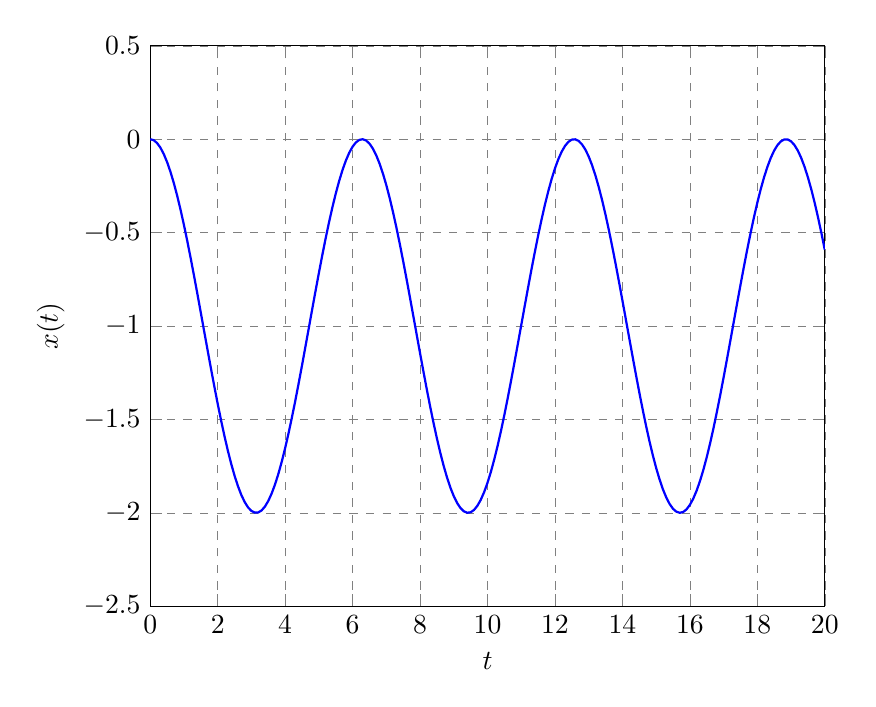
\begin{tikzpicture} \begin{axis}
[scale=1.25,
 xmin=0,    xmax=20,
 ymin=-2.5, ymax=0.5,
 grid=major, 
 major grid style={color=gray,line width=0.2pt, dashed},
 xlabel=$t$,
 ylabel=$x(t)$,
]
\addplot[
   blue,
   domain=0:20,
   samples=201,
   line width=0.8pt
]
{cos(deg(x)) - 1};
\end{axis}
\end{tikzpicture}
\caption{Solution of a simple spring problem.}
\label{Fig:ode_SimpleSpringProblem}
\end{center}
\end{figure}

What makes an initial value problem as such is its domain $0 \le t < \infty$ and that the initial conditions are given at $t = 0$. This gives the property that for a linear second-order ODE, the solution always exists. Furthermore, if we find a general solution (two linearly independent solutions for the homogeneous equation and a particular solution) that satisfies the differential equation and the boundary conditions, we are guaranteed that the solution is unique. In the other class of problems we will study, called boundary value problems, it is possible to construct boundary conditions that are inconsistent with the differential equation, which would yield no solution.

%%%%%%%%%%%%%%%%%%%%%%%%%%%%%%%%%%%%%%%%%%%%%%%%%%%%%%%%%%%%%%%%%%%%%%%%%%%%%%%%%%%%%%%%%%%%%%%%
\subsection{Coupled Systems of Initial Value Problems}

As with first-order ODEs we can have coupled systems of second-order initial value problems. For example, two coupled initial value problems can be written as
\begin{align}
  &y_1''(t) + a_{11} y_1'(t) + b_{11} y_1(t) + a_{12} y_2'(t) + b_{12} y_2(t) = r_1(t), \nonumber \\
  &y_2''(t) + a_{21} y_1'(t) + b_{21} y_1(t) + a_{22} y_2'(t) + b_{22} y_2(t) = r_2(t).
\end{align}
with initial conditions on $y_1(0)$, $y_1'(0)$, $y_2(0)$, and $y_2'(0)$ given. 

There are two approaches that can be used to address this system of equations. The first method that works only for initial value problems (not boundary value problems), is to reduce the system of $N$ second order equations to a set of first order equations. If we let $v(t) = y'(t)$. We can write the above system as follows:
\begin{align}
  &y_1'(t) - v_1(t) = 0, \nonumber \\
  &y_2'(t) - v_2(t) = 0, \nonumber \\
  &v_1'(t) + a_{11} v_1(t) + b_{11} y_1(t) + a_{12} v_2(t) + b_{12} y_2(t) = r_1(t), \nonumber \\
  &v_2'(t) + a_{21} v_1(t) + b_{21} y_1(t) + a_{22} v_2(t) + b_{22} y_2(t) = r_2(t),
\end{align}
or as an equivalent linear system as
\begin{align}
  \left[ \begin{array}{c} y_1'(t) \\ y_2'(t) \\ v_1'(t) \\ v_2'(t) \\ \end{array} \right] +
  \left[ \begin{array}{r r r r}
      0  &      0 &     -1 &      0 \\
      0  &      0 &      0 &     -1 \\
  b_{11} & b_{12} & a_{11} & a_{12} \\
  b_{21} & b_{22} & a_{21} & a_{22} \\  \end{array} \right]
  \left[ \begin{array}{c} y_1(t) \\ y_2(t) \\ v_1(t) \\ v_2(t) \\ \end{array} \right] =
  \left[ \begin{array}{c} 0 \\ 0 \\ r_1(t) \\ r_2(t) \\ \end{array} \right] .
\end{align}
This linear system of first-order differential equations can be solved using the techniques discussed previously. The advantage to this approach is that there are relatively system techniques available to solve this problem. The disadvantage is that we now need to solve twice as many equations. Additionally, this technique will not work for boundary value problems, which are very common in science and engineering.

The second solution method for the system of equations is similar to what is done for one equation. First, we solve the homogeneous problem and then attempt to find a particular solutions. For systems of second-order ordinary differential equations, we will only use the method of undetermined coefficients to find the particular solutions.

%%%%%%%%%%%%%%%%%%%%%%%%%%%%%%%%%%%%%%%%%%%%%%%%%%%%%%%%%%%%%%%%%%%%%%%%%%%%%%%%%%%%%%%%%%%%%%%%
\subsection{Example: Coupled Mass-Spring System}

To illustrate, consider the scenario with two blocks of equal mass $m$ that are connected to the walls and each other by a series of springs with equal spring constants. First we will consider the case where there is no external force. Then we will consider another case with some forcing function.

\begin{figure}[htb!]
\begin{center}
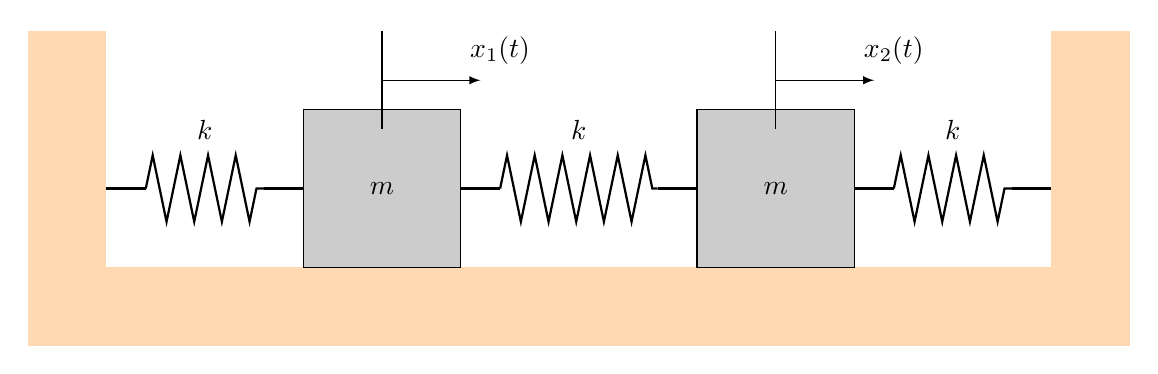
\begin{tikzpicture}
  \fill[orange!30] (0,0) -- (1,0) -- (1,4) -- (0,4) -- cycle;
  \fill[orange!30] (1,0) -- (13,0) -- (13,1) -- (1,1) -- cycle;
  \fill[orange!30] (13,0) -- (14,0) -- (14,4) -- (13,4) -- cycle;
  %
  \draw[fill=gray!40] (3.5,1) -- (5.5,1) -- (5.5,3) -- (3.5,3) -- cycle;
  \node at (4.5,2) {$m$};
  %
  \draw[fill=gray!40] (8.5,1) -- (10.5,1) -- (10.5,3) -- (8.5,3) -- cycle;
  \node at (9.5,2) {$m$};
  %
  \draw[thick] (1,2) -- (1.5,2);
  \draw[thick,decorate,decoration={zigzag,amplitude=12}] (1.5,2) -- (3,2);
  \draw[thick] (3,2) -- (3.5,2);
  \node at (2.25,2.75) {$k$};
  %
  \draw[thick] (5.5,2) -- (6,2);
  \draw[thick,decorate,decoration={zigzag,amplitude=12}] (6,2) -- (8,2);
  \draw[thick] (8,2) -- (8.5,2);
  \node at (7,2.75) {$k$};
  %
  \draw[thick] (10.5,2) -- (11,2);
  \draw[thick,decorate,decoration={zigzag,amplitude=12}] (11,2) -- (12.5,2);
  \draw[thick] (12.5,2) -- (13,2);
  \node at (11.75,2.75) {$k$};
  %
  \draw (4.5,2.75) -- (4.5,4);
  \draw[-latex] (4.5,3.375) -- (5.75,3.375);
  \node at (6,3.75) {$x_1(t)$};
  %
  \draw (9.5,2.75) -- (9.5,4);
  \draw[-latex] (9.5,3.375) -- (10.75,3.375);
  \node at (11,3.75) {$x_2(t)$};
\end{tikzpicture}
\caption{Illustration of coupled mass-spring system.}
\label{Fig:ode_coupledMassSpringExample}
\end{center}
\end{figure}

The equations of motion describing the position of the blocks for the homogeneous case are as follows:
\begin{subequations}
\begin{align}
  m x_1''(t) &= -k x_1(t) + k ( x_2(t) - x_1(t) ), \\*
  m x_2''(t) &= -k x_2(t) - k ( x_2(t) - x_1(t) ).
\end{align}
\end{subequations}
These equations can be rewritten as
\begin{subequations}
\begin{align}
  x_1''(t) + \frac{2k}{m} x_1(t) -  \frac{k}{m} x_2(t) = 0, \\*
  x_2''(t) -  \frac{k}{m} x_1(t) + \frac{2k}{m} x_2(t) = 0.
\end{align}
\end{subequations}
Since this is an oscillatory system, let us guess the following solutions:
\begin{subequations}
\begin{align}
  x_1(t) = A_1 e^{i \omega t}, \\*
  x_2(t) = A_2 e^{i \omega t}.
\end{align}
\end{subequations}
(We could guess real values in the exponential and would get to imaginary values anyway, so this simplifies matters.) Inserting this into the differential equation gives the following:
\begin{align}
  -A_1 \omega^2 + \frac{2k}{m} A_1 -  \frac{k}{m} A_2 = 0, \\*
  -A_2 \omega^2 -  \frac{k}{m} A_1 + \frac{2k}{m} A_2 = 0.
\end{align}
This linear system can be written in matrix-vector form as
\begin{align}
  \left[ \begin{array}{c c}
  \dfrac{2k}{m} - \omega^2 & -\dfrac{k}{m} \vspace{0.2cm} \\
  -\dfrac{k}{m}            & \dfrac{2k}{m} - \omega^2 \\ \end{array} \right]
  \left[ \begin{array}{c} A_1 \\ A_2 \\ \end{array} \right] =
  \left[ \begin{array}{c} 0 \\ 0 \\ \end{array} \right] .
\end{align}
To satisfy this relationship, we know the coefficients $A_1, A_2$ are zero (the trivial solution) or the determinant of the matrix is zero. This system is equivalent to an eigenvalue problem where the eigenvalue is $\omega^2$. Solving for the eigenvalues we get
\begin{align}
  \omega^2 = \left\{ \omega_1^2, \omega_2^2 \right\} = \left\{ \frac{k}{m}, \frac{3k}{m} \right\} .
\end{align}
Inserting each eigenvalue and finding the eigenvectors gives the corresponding eigenvectors
\begin{align}
  \mathbf{v}_1 = \left[ \begin{array}{c} 1 \\ 1 \\ \end{array} \right] , \quad
  \mathbf{v}_2 = \left[ \begin{array}{c} 1 \\ -1 \\ \end{array} \right] .
\end{align} 
This implies that for the first eigenvalue $\omega_1^2$, $A_1 = A_2$, and for the second eigenvalue $\omega_2^2$, $A_1 = -A_2$.

Recall that our proposed solution to differential equation was in terms of $\omega$ and not $\omega^2$, so we have
\begin{align}
  \omega_1 = \pm \sqrt{\frac{k}{m}}, \quad \omega_2 = \pm \sqrt{\frac{3k}{m}} .
\end{align}
The $\pm$ terms give us two linearly independent solutions $e^{i \omega t}$ and $e^{-i \omega t}$ with different coefficients that we will call $A_i$ and $B_i$ with $i$ corresponding to each eigenvalue. We can now write our solution as a linear combination of all terms
\begin{align}
  \left[ \begin{array}{c} x_1(t) \\ x_2(t) \\ \end{array} \right] =
  \left( A_1 e^{i \omega_1 t} + B_1 e^{-i \omega_1 t} \right) \left[ \begin{array}{c} 1 \\ 1 \\ \end{array} \right] +
  \left( A_2 e^{i \omega_2 t} + B_2 e^{-i \omega_2 t} \right) \left[ \begin{array}{c} 1 \\ -1 \\ \end{array} \right] .
\end{align}
Expanding these out gives the homogeneous solution:
\begin{subequations}
\begin{align}
  x_1(t) &= A_1 e^{i \omega_1 t} + A_2 e^{i \omega_2 t} + B_1 e^{-i \omega_1 t} + B_2 e^{-i \omega_2 t} \\*
  x_2(t) &= A_1 e^{i \omega_1 t} - A_2 e^{i \omega_2 t} + B_1 e^{-i \omega_1 t} - B_2 e^{-i \omega_2 t} .
\end{align}
\end{subequations}

Now let us consider a specific case for the homogeneous solution. Suppose we are given the initial conditions 
\begin{align}
  x_1(0)  &= 0, \nonumber \\
  x_2(0)  &= 0, \nonumber \\
  x_1'(0) &= 1, \nonumber \\
  x_2'(0) &= 0. 
\end{align}
We give the first mass a ``kick'' at time $t = 0$, but everything else is initially stationary. To apply the initial conditions we also need to velocities, which are
\begin{subequations}
\begin{align}
  x_1'(t) &= i \omega_1 A_1 e^{i \omega_1 t} + i \omega_2 A_2 e^{i \omega_2 t} - i \omega_1 B_1 e^{-i \omega_1 t} - i \omega_2 B_2 e^{-i \omega_2 t} , \\*
  x_2'(t) &= i \omega_1 A_1 e^{i \omega_1 t} - i \omega_2 A_2 e^{i \omega_2 t} - i \omega_1 B_1 e^{-i \omega_1 t} + i \omega_2 B_2 e^{-i \omega_2 t} .
\end{align}
\end{subequations}
Inserting each initial condition into the appropriate equations gives the system:
\begin{subequations}
\begin{align}
  A_1 + A_2 + B_1 + B_2 &= 0 \\
  A_1 - A_2 + B_1 - B_2 &= 0 \\
  \omega_1 A_1 + \omega_2 A_2 - \omega_1 B_1 - \omega_2 B_2 &= -i, \\
  \omega_1 A_1 - \omega_2 A_2 - \omega_1 B_1 + \omega_2 B_2 &= 0.
\end{align}
\end{subequations}
In matrix-vector form this is
\begin{align}
  \left[ \begin{array}{r r r r}
  1 &  1 & 1 &  1 \\
  1 & -1 & 1 & -1 \\
  \omega_1 &  \omega_2 & -\omega_1 & -\omega_2 \\
  \omega_1 & -\omega_2 & -\omega_1 &  \omega_1 \\ \end{array} \right]
  \left[ \begin{array}{c} A_1 \\ A_2 \\ B_1 \\ B_2 \\ \end{array} \right] =
  \left[ \begin{array}{c} 0 \\ 0 \\ -i \\ 0 \\ \end{array} \right] .
\end{align}
Let $\omega_1 = \omega$ and it follows from the eigenvalues that $\omega_2 = \sqrt{3} \omega_1 = \sqrt{3} \omega$. Solving the above system yields the solution vector
\begin{align}
  \left[ \begin{array}{c} A_1 \\ A_2 \\ B_1 \\ B_2 \\ \end{array} \right] =
  \frac{i}{4 \omega} \left[ \begin{array}{c} -1 \\ -\rfrac{1}{\sqrt{3}} \\ 1 \\ \rfrac{1}{\sqrt{3}} \\ \end{array} \right]
\end{align}

To provide numbers, suppose that $k/m = 1$; which means $\omega = 1$. Inserting the parameters into the equation gives
\begin{subequations}
\begin{align}
  x_1(t) &= \frac{i}{4} \left( -e^{i  t} - \frac{1}{\sqrt{3}} e^{i \sqrt{3} t} + e^{-i  t} + \frac{1}{\sqrt{3}} e^{-i \sqrt{3} t} \right) \\*
  x_2(t) &= \frac{i}{4} \left( -e^{i  t} + \frac{1}{\sqrt{3}} e^{i \sqrt{3} t} + e^{-i  t} - \frac{1}{\sqrt{3}} e^{-i \sqrt{3} t} \right) .
\end{align}
\end{subequations}
While these equations involve the imaginary unit $i$, they are indeed real. If we apply Euler's formula, we can express the complex exponentials in terms of trigonometric functions:
\begin{subequations}
\begin{align}
  x_1(t) &= \frac{1}{2} \sin( t ) + \frac{ 1 }{ 2 \sqrt{3} }  \sin( \sqrt{3} t ) , \\*
  x_2(t) &= \frac{1}{2} \sin( t ) - \frac{ 1 }{ 2 \sqrt{3} }  \sin( \sqrt{3} t ) .
\end{align}
\end{subequations}
These functions are plotted in Fig.~\ref{Fig:ode_CoupledSpringProblem_Homogeneous}. 

\begin{figure}[htp!]
\begin{center}
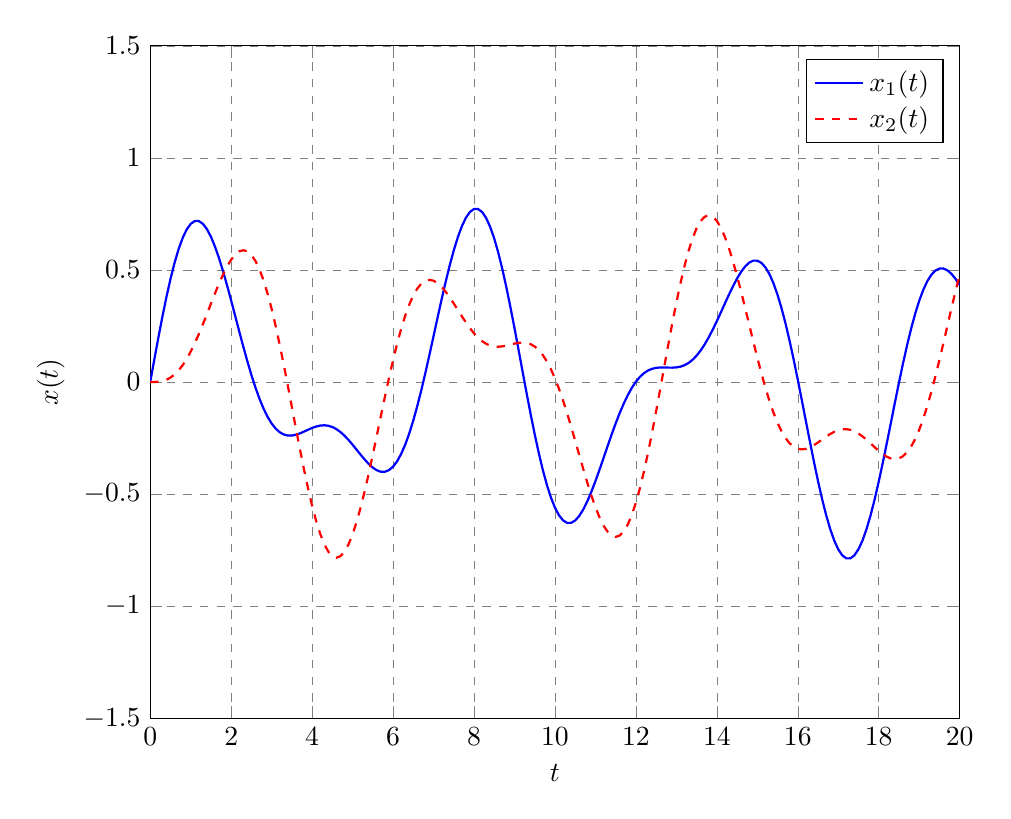
\begin{tikzpicture} \begin{axis}
[scale=1.5,
 xmin=0,    xmax=20,
 ymin=-1.5, ymax=1.5,
 grid=major, 
 major grid style={color=gray,line width=0.2pt, dashed},
 xlabel=$t$,
 ylabel=$x(t)$,
]
\addplot[
   blue,
   domain=0:20,
   samples=201,
   line width=0.8pt
]
{0.5*sin(deg(x)) + 1/(2*sqrt(3))*sin(sqrt(3)*deg(x))};
\addlegendentry{$x_1(t)$};
\addplot[
   red,
   domain=0:20,
   samples=201,
   line width=0.8pt,
   dashed
]
{0.5*sin(deg(x)) - 1/(2*sqrt(3))*sin(sqrt(3)*deg(x))};
\addlegendentry{$x_2(t)$};
\end{axis}
\end{tikzpicture}
\caption{Solution of a homogeneous coupled mass-spring problem.}
\label{Fig:ode_CoupledSpringProblem_Homogeneous}
\end{center}
\end{figure}

Now let us suppose we apply an exponential forcing function to the block~1. This leads to a new set of differential equations as follows:
\begin{subequations}
\begin{align}
  x_1''(t) + \frac{2k}{m} x_1(t) -  \frac{k}{m} x_2(t) = e^{-\gamma t}, \\*
  x_2''(t) -  \frac{k}{m} x_1(t) + \frac{2k}{m} x_2(t) = 0.
\end{align}
\end{subequations}
The homogeneous solution is identical to what we found before. To find the particular solution, we apply the method of underdetermined coefficients. Since the inhomogeneous solution is exponential, we guess an exponential:
\begin{subequations}
\begin{align}
  x_1(t) = c_1 e^{-\gamma t}, \\*
  x_2(t) = c_2 e^{-\gamma t}.
\end{align}
\end{subequations}
Plugging these into the differential equations and canceling out the exponential yields the system
\begin{subequations}
\begin{align}
  \gamma^2 c_1 + \frac{2k}{m} c_1 -  \frac{k}{m} c_2 = 1, \\*
  \gamma^2 c_2 - \frac{k}{m}  c_1 + \frac{2k}{m} _2 = 0.
\end{align}
\end{subequations}
We can write this in matrix-vector form as
\begin{align}
  \left[ \begin{array}{c c}
  \gamma^2 + \dfrac{2k}{m} & -\dfrac{k}{m} \vspace{0.2cm} \\
  -\dfrac{k}{m} & \gamma^2 + \dfrac{2k}{m} \\ \end{array} \right]
  \left[ \begin{array}{c} c_1 \\ c_2 \\ \end{array} \right] =
  \left[ \begin{array}{c} 1 \\ 0 \\ \end{array} \right] .
\end{align}
Solving this system yields the solution vector
\begin{align}
  \left[ \begin{array}{c} c_1 \\ c_2 \\ \end{array} \right] =
  \left[ \begin{array}{c} 
  \dfrac{ \gamma^2 + \rfrac{2k}{m} }{ ( \gamma^2 + \rfrac{2k}{m} )^2 - \rfrac{k^2}{m^2} } \vspace{0.2cm} \\* 
  \dfrac{ \rfrac{k}{m} }{ ( \gamma^2 + \rfrac{2k}{m} )^2 - \rfrac{k^2}{m^2} } \\ \end{array} \right] .
\end{align}
The general solution is therefore (leaving in terms of constants $c_1$ and $c_2$ since it is rather unwieldy):
\begin{subequations}
\begin{align}
  x_1(t) &= A_1 e^{i \omega_1 t} + A_2 e^{i \omega_2 t} + B_1 e^{-i \omega_1 t} + B_2 e^{-i \omega_2 t} + c_1 e^{-\gamma t} , \\*
  x_2(t) &= A_1 e^{i \omega_1 t} - A_2 e^{i \omega_2 t} + B_1 e^{-i \omega_1 t} - B_2 e^{-i \omega_2 t} + c_2 e^{-\gamma t} .
\end{align}
\end{subequations}
Taking derivatives to get the velocity terms gives
\begin{subequations}
\begin{align}
  x_1'(t) &= i \omega_1 A_1 e^{i \omega_1 t} + i \omega_2 A_2 e^{i \omega_2 t} - i \omega_1 B_1 e^{-i \omega_1 t} - i \omega_2 B_2 e^{-i \omega_2 t} - \gamma c_1 e^{-\gamma t} , \\*
  x_2'(t) &= i \omega_1 A_1 e^{i \omega_1 t} - i \omega_2 A_2 e^{i \omega_2 t} - i \omega_1 B_1 e^{-i \omega_1 t} + i \omega_2 B_2 e^{-i \omega_2 t} - \gamma c_2 e^{-\gamma t} .
\end{align}
\end{subequations}

Before moving onto discussing an example with an inhomogeneous term and obtaining the particular solution, let us connect this to eigenvalues and eigenvectors from linear algebra. To begin solving the problem, we calculated the eigenvalues of the system. In the context of mass-spring systems or harmonic oscillators, these eigenvalues correspond to the natural frequencies of the system. For each of these eigenvalues (natural frequencies) we obtained a vector of \emph{eigenfunctions} that are proportional to $e^{\pm i \omega_k t}$ that could then be expressed in terms of trigonometric functions. Eigenfunctions are the continuous analog in calculus to the eigenvectors in linear algebra. As we applied the initial conditions, note that the homogeneous solution is a linear combination of the eigenfunctions, which here can be expressed as either complex exponentials or trigonometric functions. The ability to express a homogeneous solution as a linear combinations of its eigenfunctions is a general result to differential equations and an important idea.

Next let us consider a case with an inhomogeneous term. Suppose that again $k/m = 1$ and now $\gamma = 1$. The coefficients for the particular solution are $c_1 = \rfrac{3}{8}$ and $c_2 = \rfrac{1}{8}$. Furthermore, we will assume that the positions and velocities are now initially zero:
\begin{align}
  x_1(0)  &= 0, \nonumber \\
  x_2(0)  &= 0, \nonumber \\
  x_1'(0) &= 0, \nonumber \\
  x_2'(0) &= 0. 
\end{align}
Applying these initial conditions yields the system
\begin{subequations}
\begin{align}
  A_1 + A_2 + B_1 + B_2 &= -\frac{3}{8} \\
  A_1 - A_2 + B_1 - B_2 &= -\frac{1}{8} \\
  A_1 + \sqrt{3} A_2 - B_1 - \sqrt{3} B_2 &= -\frac{3i}{8}, \\
  A_1 - \sqrt{3} A_2 - B_1 + \sqrt{3} B_2 &= -\frac{i}{8}.
\end{align}
\end{subequations}
The corresponding matrix-vector form is
\begin{align}
  \left[ \begin{array}{r r r r}
  1 &  1 & 1 &  1 \\
  1 & -1 & 1 & -1 \\
  1 &  \sqrt{3} & -1 & -\sqrt{3} \\
  1 & -\sqrt{3} & -1 &  \sqrt{3} \\ \end{array} \right]
  \left[ \begin{array}{c} A_1 \\ A_2 \\ B_1 \\ B_2 \\ \end{array} \right] =
  \left[ \begin{array}{c} -\rfrac{3}{8} \\ -\rfrac{1}{8} \\ -\rfrac{3i}{8} \\ -\rfrac{i}{8} \\ \end{array} \right] .
\end{align}
The solution vector is
\begin{align}
  \left[ \begin{array}{c} A_1 \\ A_2 \\ B_1 \\ B_2 \\ \end{array} \right] =
  -\frac{1}{8} \left[ \begin{array}{c} 1 + i \\ \frac{1}{2} + \frac{i}{2 \sqrt{3}} \\ 1 - i \\ \frac{1}{2} - \frac{i}{2 \sqrt{3}} \\ \end{array} \right] .
\end{align}
Plugging in the values and applying Euler's formula gives the result:
\begin{subequations}
\begin{align}
  x_1(t) &= \frac{1}{4} \sin( t ) - \frac{1}{4} \cos( t ) + \frac{ 1 }{ 8 \sqrt{3} } \sin( \sqrt{3} t ) - \frac{1}{8} \cos( \sqrt{3} t ) + \frac{3}{8} e^{-t} , \\*
  x_2(t) &= \frac{1}{4} \sin( t ) - \frac{1}{4} \cos( t ) - \frac{ 1 }{ 8 \sqrt{3} } \sin( \sqrt{3} t ) + \frac{1}{8} \cos( \sqrt{3} t ) + \frac{1}{8} e^{-t} .
\end{align}
\end{subequations}
This solution is plotted in Fig.~\ref{Fig:ode_CoupledSpringProblem_ExponentialForcing}. As before, we have the homogeneous solution expressed as a linear combination of eigenfunctions (this time with different coefficients) with an added term because of the forcing function.

\begin{figure}[htp!]
\begin{center}
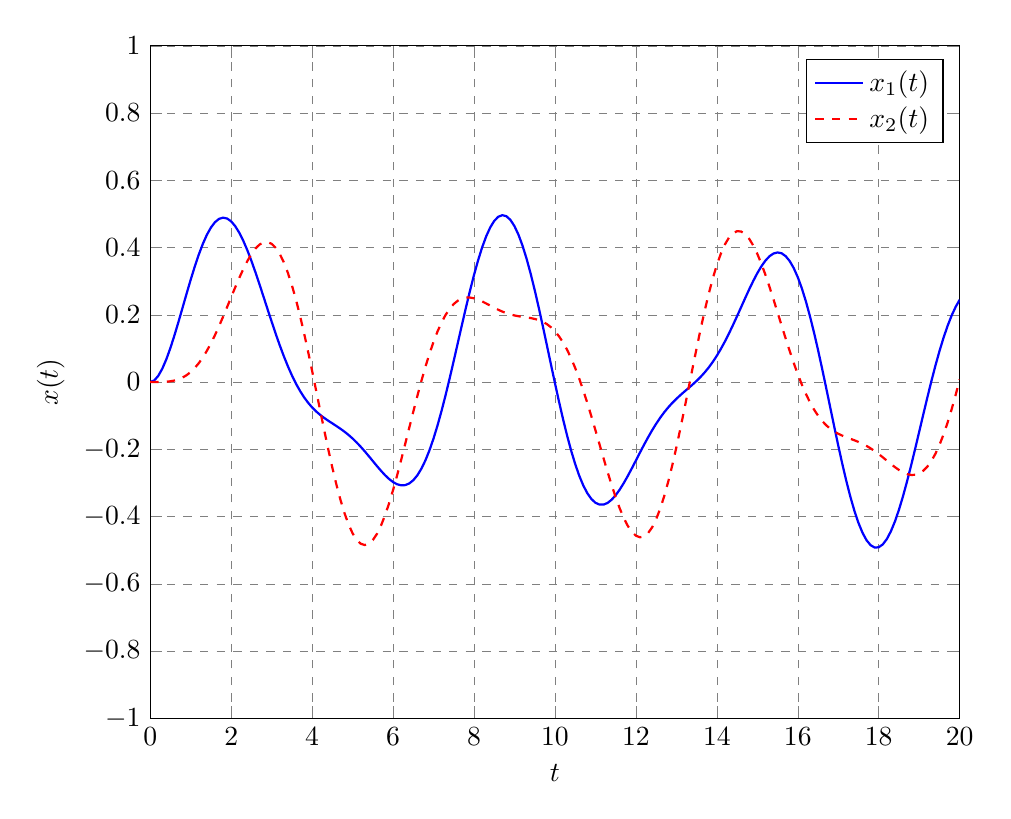
\begin{tikzpicture} \begin{axis}
[scale=1.5,
 xmin=0,    xmax=20,
 ymin=-1, ymax=1,
 grid=major, 
 major grid style={color=gray,line width=0.2pt, dashed},
 xlabel=$t$,
 ylabel=$x(t)$,
]
\addplot[
   blue,
   domain=0:20,
   samples=201,
   line width=0.8pt
]
{0.25*sin(deg(x)) - 0.25*cos(deg(x)) + 1/(8*sqrt(3))*sin(sqrt(3)*deg(x)) - 1/8*cos(sqrt(3)*deg(x)) + 3/8*exp(-x) };
\addlegendentry{$x_1(t)$};
\addplot[
   red,
   domain=0:20,
   samples=201,
   line width=0.8pt,
   dashed
]
{0.25*sin(deg(x)) - 0.25*cos(deg(x)) - 1/(8*sqrt(3))*sin(sqrt(3)*deg(x)) + 1/8*cos(sqrt(3)*deg(x)) + 1/8*exp(-x)};
\addlegendentry{$x_2(t)$};
\end{axis}
\end{tikzpicture}
\caption{Solution of a coupled mass-spring problem with an exponential forcing function.}
\label{Fig:ode_CoupledSpringProblem_ExponentialForcing}
\end{center}
\end{figure}

%%%%%%%%%%%%%%%%%%%%%%%%%%%%%%%%%%%%%%%%%%%%%%%%%%%%%%%%%%%%%%%%%%%%%%%%%%%%%%%%%%%%%%%%%%%%%%%%
%%%%%%%%%%%%%%%%%%%%%%%%%%%%%%%%%%%%%%%%%%%%%%%%%%%%%%%%%%%%%%%%%%%%%%%%%%%%%%%%%%%%%%%%%%%%%%%%
\section{Boundary Value Problems}

The other major and important class of problems for differential equations are boundary value problems. Boundary value problems involving second-order ordinary differential equation are ubiquitous and appear in fields ranging from: fluid dynamics, heat transfer, neutron transport and reactor physics, plasma physics, materials science, and quantum mechanics to name a few.

The difference of a boundary value problem versus an initial value problem is now the problem is defined over some domain with boundary conditions applied at the exterior as opposed to from $0 \le t \le \infty$ with initial conditions given at $t = 0$ The system could be infinite $-\infty < x < \infty$, semi-infinite similar to initial value problems $a \le x < \infty$, or finite $a \le x \le b$. In boundary value problems, boundary conditions are provided, as the name implies, at the exterior boundaries of the system and these can be in terms of the function, its derivative, or a linear combination thereof. It is also common that for many problems in science and engineering the interior of the problem has discrete regions, often representing different objects or materials, and these are treated mathematically with interface conditions. Once we have the boundary and interface conditions, we can set up a system of equations for the boundary value problem and attempt to solve. 

%%%%%%%%%%%%%%%%%%%%%%%%%%%%%%%%%%%%%%%%%%%%%%%%%%%%%%%%%%%%%%%%%%%%%%%%%%%%%%%%%%%%%%%%%%%%%%%%
\subsection{Boundary Conditions}

Boundary conditions are specified at the edges of the problem domain and are necessary to have a well-posed problem. There are three major types of boundary conditions that appear in most science and engineering applications: the Dirichlet boundary condition, the Neumann boundary condition, and the Robbin boundary condition.

The Dirichlet boundary condition is the simplest type and specifies the solution of the field at some boundary point $x_b$:
\begin{align}
  f(x_b) = c.
\end{align}
For example, in heat conduction problems we are often interested in solving for the distribution of temperatures, or the temperature field. In many cases the temperature at one of the boundaries is known. Also in fluids problems, we often specify the ''no-slip condition'' that says the velocity of the fluid is zero at the walls.

The Neumann boundary condition specifies the first derivative of the solution of the field at some boundary point $x_b$:
\begin{align}
  f'(x_b) = c.
\end{align}
A common example occurs in heat condition where rather than the temperature $T$ being specified on the boundary, we have a known heat flux $q$, which is proportional to the derivative of the temperature,
\begin{align}
  q = -k \frac{dT}{dx}.
\end{align}
Another important place where the Neumann boundary condition arises is when we are applying symmetry to a problem. It is often the case that it is easier to solve a portion of a much larger problem where that portion is replicated in a way that we have symmetry. In these cases, it is often the case that derivatives are zero at boundaries for symmetry. We often refer to this as a ``reflecting boundary condition'' or ``symmetry boundary condition''.

The third important type of boundary condition is the Robin boundary condition, which specifies a linear combination of the field and its first derivative are given on the boundary:
\begin{align}
  a f(x_b) + b f'(x_b) = c.
\end{align}
A common example of this in heat conduction involves a convective boundary condition, where energy is transferred to the ambient medium. This is often written as
\begin{align}
  q = h ( T - T_\infty ),
\end{align}
where $h$ is a heat transfer coefficient and $T_\infty$ is the ambient temperature ``infinitely'' far away from the heated object being analyzed. To see this is equivalent to the form of the Robin boundary condition, let us expand the heat flux and rearrange:
\begin{align}
  \frac{k}{h} T'(x_b) + T(x_b) = T_\infty .
\end{align}
The other place in nuclear engineering where this comes up is neutron diffusion in reactors, which is called the Marshak boundary condition. Here we wish to know about the neutron path-length rate density (or neutron scalar flux, which is proportional to the nuclear reaction rate) $\phi(x)$ at the boundary. This is given as
\begin{align}
   \frac{1}{4} \phi(x_b) \mp \frac{D}{2} \phi'(x_b) = J^{\pm}(x_b). 
\end{align}
Here $J^+(x_b)$ and $J^-(x_b)$ are the given neutron currents (flow rate of neutrons) given on the left and right sides of the problem respectively; $D$ is the neutron diffusion coefficient describing the magnitude of the ability for neutrons to spread out within a given medium. Note that the $\pm$ and $\mp$ symbols mean that when one side uses the $+$ the other uses the $-$ and vice versa.

There is another class of boundary condition that often occurs. It is often the case that we must assert that the field is finite or tends toward zero as the field goes out toward infinity (in other words, the field does not ``blow up'' for large magnitude in $x$). Also, when we are in cylindrical or spherical geometry, we often must assert that the field is finite at the boundary.

%%%%%%%%%%%%%%%%%%%%%%%%%%%%%%%%%%%%%%%%%%%%%%%%%%%%%%%%%%%%%%%%%%%%%%%%%%%%%%%%%%%%%%%%%%%%%%%%
\subsection{Interface Conditions}

Within the interior of the problem, we must specify how the field and its derivative are connected to adjacent regions. It is often the case that the field is continuous. If we have an interface point $a$ between regions 1 and 2, the interface condition for the field is often
\begin{align}
  f_1(a) = f_2(a).
\end{align}
Note that it is possible in certain situations, e.g., shock waves that are important in inertial confinement fusion, to have a discontinuity in the field; this is called a jump condition.

We also must often specify some condition on the derivative at the interface. Physically, this means that the flow rate of some physical quantity (e.g., energy, neutrons, etc.) related to the first derivative of the field (e.g., heat flux, neutron current, respectively) is continuous across the boundary. Because the flow rates of these properties often depend directly upon some property in the system, the derivative of the field is often discontinuous and exhibits a ``kink''. This interface condition is often written as
\begin{align}
  k_1 f_1'(a) = k_2 f_2'(a).
\end{align}
Sometimes there can be an added inhomogeneous constant value as well (analogous to a jump condition). This can, for example, denote a source of energy at the boundary or a surface charge in electrostatics.

The derivation of these conditions involves integrating the differential equation over some small range $\pm \epsilon$ around the interface and taking the limit as $\epsilon \rightarrow 0$. Consider the following diffusion equation at an interface
\begin{align}
  -\frac{d}{dx} \left( D(x) \frac{d\phi}{dx} \right) + \Sigma_a(x) \phi(x) = Q(x),
\end{align}
where the diffusion coefficient is
\begin{align}
  D(x) = \left\{ \begin{array}{c l} D_1 & x < a, \\
                                    D_2 & x > a, \\ \end{array} \right. .
\end{align}
If we wish to derive an interface condition, we integrate from $a - \epsilon$ to $a + \epsilon$:
\begin{align}
  - \int_{a-\epsilon}^{a+\epsilon} \frac{d}{dx} \left( D(x) \frac{d\phi}{dx} \right) + \int_{a-\epsilon}^{a+\epsilon} \Sigma_a(x) \phi(x) = \int_{a-\epsilon}^{a+\epsilon} Q(x).
\end{align}
Using the second fundamental theorem of calculus on the first term yields
\begin{align}
  - \left[  D_2 \phi_2'(a + \epsilon) -  D_1 \phi_1'(a - \epsilon) \right] + \int_{a-\epsilon}^{a+\epsilon} \Sigma_a(x) \phi(x) = \int_{a-\epsilon}^{a+\epsilon} Q(x).
\end{align}
Now, we take the limit as $\epsilon \rightarrow 0$. The integrals that remain go to zero and we are left with:
\begin{align}
  - \left[  D_2 \phi_2'(a) -  D_1 \phi_1'(a) \right] = 0.
\end{align}

%%%%%%%%%%%%%%%%%%%%%%%%%%%%%%%%%%%%%%%%%%%%%%%%%%%%%%%%%%%%%%%%%%%%%%%%%%%%%%%%%%%%%%%%%%%%%%%%
\subsection{Example: Flow Between Two Parallel Plates}

Consider a fluid flowing between two plates in a rectangular duct with a width $2L$ such that $-L \le x \le L$ and very wide in the $y$ and $z$ directions so that we can ignore the effects of the boundaries in those directions. The flow is driven by a constant pressure gradient in the $y$ direction driven by gravity:
\begin{align}
  \frac{dp}{dy} = \rho g.
\end{align}
The equations describing the velocity profile in the $y$ direction, $v_y(x)$ is given as
\begin{align}
  \mu \frac{d^2 v_y}{dx^2} = \frac{dp}{dy} = \rho g;
\end{align}
Here $\mu$ is the fluid viscosity that represents the friction generated within the fluid. The fluid velocity profile is assumed to satisfy the no-slip condition, so
\begin{subequations}
\begin{align}
  v_y(-L) &= 0, \\*
  v_y(L) &= 0.
\end{align}
\end{subequations}
The differential equation is simple to solve, as it can be integrated twice. This yields a solution in terms of two constants of iteration:
\begin{align}
  v_y(x) = \frac{\rho g x^2}{2 \mu} + C_1 x + C_2.
\end{align}
Inserting in the boundary conditions gives
\begin{subequations}
\begin{align}
  v_y(-L) &= \frac{\rho g L^2}{2 \mu}  - C_1 L + C_2 = 0, \\*
  v_y(L)  &= \frac{\rho g L^2}{2 \mu} + C_1 L + C_2 = 0.
\end{align}
\end{subequations}
Writing a linear system in matrix-vector form gives
\begin{align}
  \left[ \begin{array}{r r}
  -L &  1 \\
   L &  1 \\ \end{array} \right]
   \left[ \begin{array}{c} C_1 \\ C_2 \\ \end{array} \right] =
   -\frac{\rho g L^2}{2\mu} \left[ \begin{array}{c} 1 \\ 1 \\ \end{array} \right] .
\end{align}
Solving this system yields
\begin{subequations}
\begin{align}
  C_1 &= 0. \\
  C_2 &= -\frac{\rho g L^2}{2 \mu} .
\end{align}
\end{subequations}
Inserting this into the equation gives the final result
\begin{align}
  v_y(x) = -\frac{\rho g L^2}{2 \mu} \left[ 1 - \left( \frac{y}{L} \right)^2 \right] .
\end{align}
The flow is negative because gravity points in the downward direction and has a parabolic shape with the maximum being at the centerline $x = 0$. The velocity profile is depicted in Fig.~\ref{Fig:ode_fluidFlowParallelPlatesExample}.

\begin{figure}[tb!]
\begin{center}
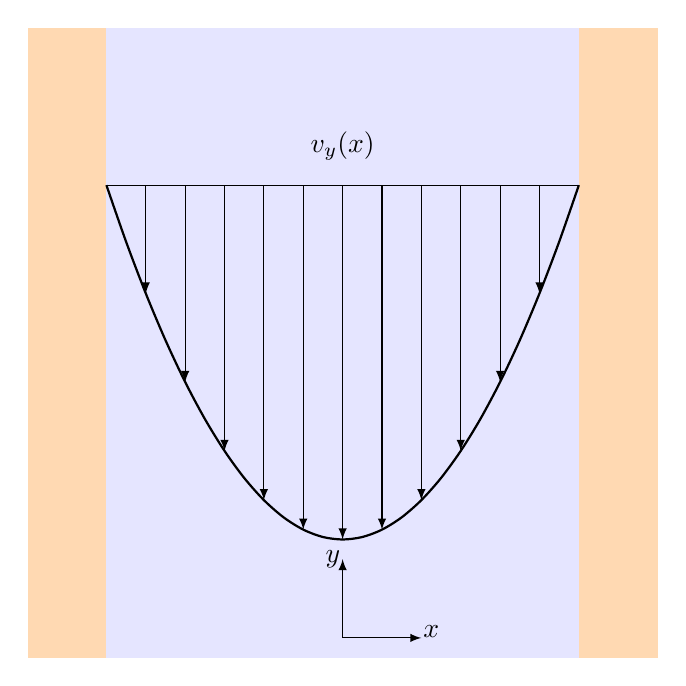
\begin{tikzpicture}
  \fill[orange!30] (-4,0) -- (-3,0) -- (-3,8) -- (-4,8) -- cycle;
  \fill[blue!10]   (-3,0) -- (3,0) -- (3,8) -- (-3,8) -- cycle;
  \fill[orange!30] ( 3,0) -- (4,0) -- (4,8) -- (3,8) -- cycle;
  \draw[thick]   plot[smooth,domain=-3:3] (\x, {1.5+0.5*\x*\x});
  \draw (-3,6) -- (3,6);
  \foreach \x in {-2.5,-2.0,-1.5,-1.0,-0.5,0.0,0.5,1.0,1.5,2.0,2.5}
    \draw[-latex] (\x,6)   -- (\x,{1.5 + 0.5*\x*\x});
  \node at (0,6.5) {$v_y(x)$};
  \draw[-latex] (0,0.25) -- (1,0.25);
  \draw[-latex] (0,0.25) -- (0,1.25);
  \node at (1.125,0.325) {$x$};
  \node at (-0.125,1.25) {$y$};
%  \draw[fill=gray!40] (3.5,1) -- (5.5,1) -- (5.5,3) -- (3.5,3) -- cycle;
%  \draw[fill=gray!40] (8.5,1) -- (10.5,1) -- (10.5,3) -- (8.5,3) -- cycle;
%  \draw[thick] (1,2) -- (1.5,2);
%  \draw[thick,decorate,decoration={zigzag,amplitude=12}] (1.5,2) -- (3,2);
%  \draw[thick] (3,2) -- (3.5,2);
%  \draw[thick] (5.5,2) -- (6,2);
%  \draw[thick,decorate,decoration={zigzag,amplitude=12}] (6,2) -- (8,2);
%  \draw[thick] (8,2) -- (8.5,2);
%  \draw[thick] (10.5,2) -- (11,2);
%  \draw[thick,decorate,decoration={zigzag,amplitude=12}] (11,2) -- (12.5,2);
%  \draw[thick] (12.5,2) -- (13,2);
\end{tikzpicture}
\caption{Illustration of velocity profile between two parallel plates.}
\label{Fig:ode_fluidFlowParallelPlatesExample}
\end{center}
\end{figure}

%%%%%%%%%%%%%%%%%%%%%%%%%%%%%%%%%%%%%%%%%%%%%%%%%%%%%%%%%%%%%%%%%%%%%%%%%%%%%%%%%%%%%%%%%%%%%%%%
\subsection{Example: Heat Conduction in a Nuclear Fuel Rod} \label{Sec:ode_boundaryValues_heatConductionExample}

An important parameter for nuclear fission reactor analysis is modeling the energy transport in the reactor. Part of this is finding the temperature field within a fuel pin to ensure that the temperature throughout the fuel and cladding stays below materials limit that could damage the cladding and lead to a subsequent release of radioactive fission products into the coolant. 

A fuel pin is a cylindrical object (depicted in Fig.~\ref{Fig:ode_nuclearFuelRodGeometry}) with a diameter of about 1~cm with the uranium dioxide fuel being about 0.8~cm in diameter, cladding on the outside being about 0.05~cm in thickness, and the area between being a fill gas that has a low thermal conductivity. The fuel is surrounded by water where the heat is removed through forced convection. 

\begin{figure}[tb!]
\begin{center}
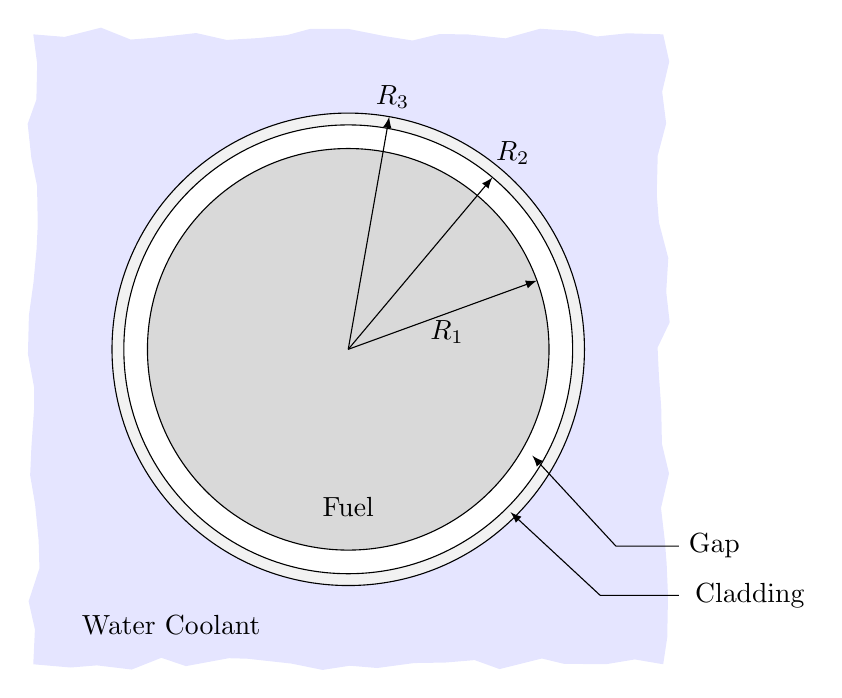
\begin{tikzpicture}
  \fill[blue!10, decoration={random steps,segment length=0.4cm}] (-4,-4) decorate{-- (+4,-4)} decorate{-- (+4,+4)} decorate{-- (-4,+4)} decorate{-- cycle};
  \draw[fill=gray!10] (0,0) circle (3cm);
  \draw[fill=white]   (0,0) circle (2.85cm);
  \draw[fill=gray!30] (0,0) circle (2.55cm);
  \node at (-2.25,-3.5) {Water Coolant};
  \node at (0,-2)    {Fuel};
  \node at (4.65,-2.5)  {Gap};
  \node at (5.1,-3.125) {Cladding};
  \draw[-latex] (4.2,-2.5) -- (3.4,-2.5) -- (2.338,-1.350);
  \draw[-latex] (4.2,-3.125) -- (3.2,-3.125) -- (2.0608,-2.0680);
  \draw[-latex] (0,0) -- (2.396,0.872);
  \draw[-latex] (0,0) -- (1.832,2.183);
  \draw[-latex] (0,0) -- (0.521,2.954);
  \node at (0.564,3.201) {$R_3$};
  \node at (2.089,2.490) {$R_2$};
  \node at (1.255,0.221) {$R_1$};
\end{tikzpicture}
\caption{Illustration of a nuclear fuel rod in coolant.}
\label{Fig:ode_nuclearFuelRodGeometry}
\end{center}
\end{figure}


We will solve a simplified version of this problem where we only consider the radial dependence and neglect any axial power dependence. In cylindrical geometry, the equation for heat conduction within a region is given by
\begin{align}
  -\frac{k}{r} \frac{d}{dr} \left( r \frac{dT}{dr} \right) = Q(r),
\end{align}
where $r$ is the radial coordinate, $k$ is the thermal conductivity that we assume to be independent of temperature and constant within each region, and $Q(r)$ is the heat generation distribution.

Within the fuel, which we denote as region 1, we assume the heat generation is spatially constant $Q_1(r) = Q_1$. The differential equation becomes:
\begin{subequations}
\begin{align}
  -\frac{k_1}{r} \frac{d}{dr} \left( r \frac{dT}{dr} \right) &= Q_1.
\end{align}
In the gap and cladding (regions 2 and 3 respectively), there is no heat generation $Q_2(r) = 0, Q_3(r) = 0$. This leads to the equations:
\begin{align}
  -\frac{k_2}{r} \frac{d}{dr} \left( r \frac{dT}{dr} \right) &= 0, \\
  -\frac{k_3}{r} \frac{d}{dr} \left( r \frac{dT}{dr} \right) &= 0.
\end{align}
\end{subequations}
We have three second-order ordinary differential equations that all require a total of six constraints. For the fuel region, we require that at the origin, $r = 0$, is finite:
\begin{subequations}
\begin{align}
  T_1(0) < \infty.
\end{align}
Next, we require two interface conditions between the fuel and gap being that the temperature and heat flux are continuous across the interface:
\begin{align}
  T_1(R_1) &= T_2(R_1), \\
  q_1(R_1) &= q_2(R_1).
\end{align}
Likewise, the same interface conditions apply between the gap and cladding:
\begin{align}
  T_2(R_2) &= T_3(R_2), \\
  q_2(R_2) &= q_3(R_2).
\end{align}
Finally, on the outer surface of the cladding, the energy is removed by the coolant via the convection process. Here we apply the convective boundary condition:
\begin{align}
  q_3(R_3) &= h ( T_3(R_3) - T_\infty ).
\end{align}
\end{subequations}
As with the previous example, these equations can be integrated twice directly. The results are:
\begin{subequations}
\begin{align}
  T_1(r) &= -\frac{Q_1}{4k_1} r^2 + A_1 \ln( r ) + B_1, \\
  T_2(r) &= A_2 \ln( r ) + B_2, \\
  T_3(r) &= A_3 \ln( r ) + B_3.
\end{align}
\end{subequations}
Applying the condition that $T_1(0)$ is finite requires that $A_1 = 0$ since $\ln( r ) \rightarrow -\infty$ as $r \rightarrow 0$. Given that simplification, let us compute the heat fluxes:
\begin{subequations}
\begin{align}
  q_1(r) &= -k_1 \frac{dT_1}{dr} = \frac{Q_1}{2} r, \\
  q_2(r) &= -k_2 \frac{dT_2}{dr} = -k_2 A_2 \frac{1}{r}, \\
  q_3(r) &= -k_3 \frac{dT_2}{dr} = -k_3 A_3 \frac{1}{r}.
\end{align}
\end{subequations}
Applying the interface condition for the temperature between the fuel and gap gives
\begin{align}
  -\frac{Q_1}{4k_1} R_1^2 + B_1 = A_2 \ln( R_1 ) + B_2.
\end{align}
Moving all the coefficients to the left-hand side and everything else to the right-hand side gives
\begin{align}
  B_1 - \ln( R_1 ) A_2 - B_2 = \frac{Q_1 R_1^2}{4k_1} .
\end{align}
Applying the corresponding heat flux equation gives
\begin{align}
  -k_2 A_2 \frac{1}{R_1} = \frac{Q_1 R_1}{2} 
\end{align}
Solving for $A_2$ explicitly gives
\begin{align}
  A_2 = -\frac{Q_1 R_1^2}{2 k_2}  .
\end{align}

Next, applying the temperature interface condition to gap/clad interface gives
\begin{align}
   A_2 \ln( R_2 ) + B_2 = A_3 \ln( R_2 ) + B_3.
\end{align}
Grouping terms gives
\begin{align}
   \ln( R_2 ) A_2  + B_2 - \ln( R_2 ) A_3  - B_3 = 0.
\end{align}
The corresponding heat flux condition is
\begin{align}
   k_2 A_2  - k_3 A_3 = 0
\end{align}
Solving for $A_3$ is straightforward:
\begin{align}
  A_3 = -\frac{Q_1 R_1^2}{2 k_3}.
\end{align}

Finally, we apply the convective boundary condition to the outer surface of the cladding:
\begin{align}
  -k_3 A_3 \frac{1}{R_3} &= h \left( A_3 \ln( R_3 ) + B_3 - T_\infty \right).
\end{align}
Rearranging terms gives
\begin{align}
  \left( \ln(R_3) +  \frac{k_3}{h R_3} \right) A_3 + B_3 = T_\infty .
\end{align}
Collecting these into a linear system gives
\begin{align}
  \left[ \begin{array}{c c c c c c}
  1 & 0 &         0 &  0 &         0 &  0 \\
  0 & 1 & -\ln(R_1) & -1 &         0 &  0 \\
  0 & 0 &         1 &  0 &         0 &  0 \\
  0 & 0 &  \ln(R_2) &  1 & -\ln(R_2) & -1 \\
  0 & 0 &         0 &  0 &         1 &  0 \\
  0 & 0 &         0 &  0 & \ln(R_3) + \frac{k_3}{h R_3} & 1 \\ \end{array} \right]
  \left[ \begin{array}{c} A_1 \\ B_1 \\ A_2 \\ B_2 \\ A_3 \\ B_3 \end{array} \right] =
  \left[ \begin{array}{c}                        0 \\ \frac{Q_1 R_1^2}{4 k_1} \\ 
                          -\frac{Q_1 R_1^2}{2 k_2} \\ 0 \\
                          -\frac{Q_1 R_1^2}{2 k_3} \\ T_\infty \\ \end{array} \right] .
\end{align}
We can then apply Gaussian elimination to solve this system. The following coefficients are obtained:
\begin{subequations}
\begin{align}
  A_1 &= 0, \\*
  B_1 &= T_\infty + \frac{Q_1 R_1^2}{2} \left[ \frac{1}{2k_1} + \frac{1}{k_2} \ln \left( \frac{R_2}{R_1} \right) 
                                             + \frac{1}{k_3} \ln \left( \frac{R_3}{R_2} \right)  + \frac{1}{h R_3} \right], \\*
  A_2 &= -\frac{Q_1 R_1^2}{2 k_2}, \\*
  B_2 &= T_\infty + \frac{Q_1 R_1^2}{2} \left[ \frac{1}{k_2} \ln(R_2) + \frac{1}{k_3} \ln \left( \frac{R_3}{R_2} \right) + \frac{1}{h R_3} \right] . \\*
  A_3 &= -\frac{Q_1 R_1^2}{2 k_3}, \\*
  B_3 &= T_\infty + \frac{Q_1 R_1^2}{2} \left[ \frac{1}{k_3} \ln(R_3) + \frac{1}{h R_3} \right] .
\end{align}
\end{subequations}
The temperature field solution is therefore:
\begin{subequations}
\begin{align}
%  T_1(t) &= T_\infty + \frac{Q_1 R_1^2}{2} \left[ \frac{1}{2k_1} \left( 1 - \left( \frac{r}{R_1} \right)^2 \right) 
%          + \frac{1}{k_2} \ln \left( \frac{R_2}{R_1} \right) + \frac{1}{k_3} \ln \left( \frac{R_3}{R_2} \right)  + \frac{1}{h R_3} \right] \\
  T_1(r) &= T_\infty + \frac{Q_1 R_1^2}{4k_1} \left[ 1 - \left( \frac{r}{R_1} \right)^2 \right] \nonumber \\*
         &+ \frac{Q_1 R_1^2}{2} \left[ \frac{1}{k_2} \ln \left( \frac{R_2}{R_1} \right) 
          + \frac{1}{k_3} \ln \left( \frac{R_3}{R_2} \right)  + \frac{1}{h R_3} \right] , \\*
  T_2(r) &= T_\infty + \frac{Q_1 R_1^2}{2} \left[ \frac{1}{k_2} \ln \left( \frac{R_2}{r} \right) + \frac{1}{k_3} \ln \left( \frac{R_3}{R_2} \right) + \frac{1}{h R_3} \right] , \\*
  T_3(r) &= T_\infty + \frac{Q_1 R_1^2}{2} \left[ \frac{1}{k_3}  \ln \left( \frac{R_3}{r} \right) + \frac{1}{h R_3} \right] .
\end{align}
\end{subequations}

\begin{figure}[t!]
\begin{center}
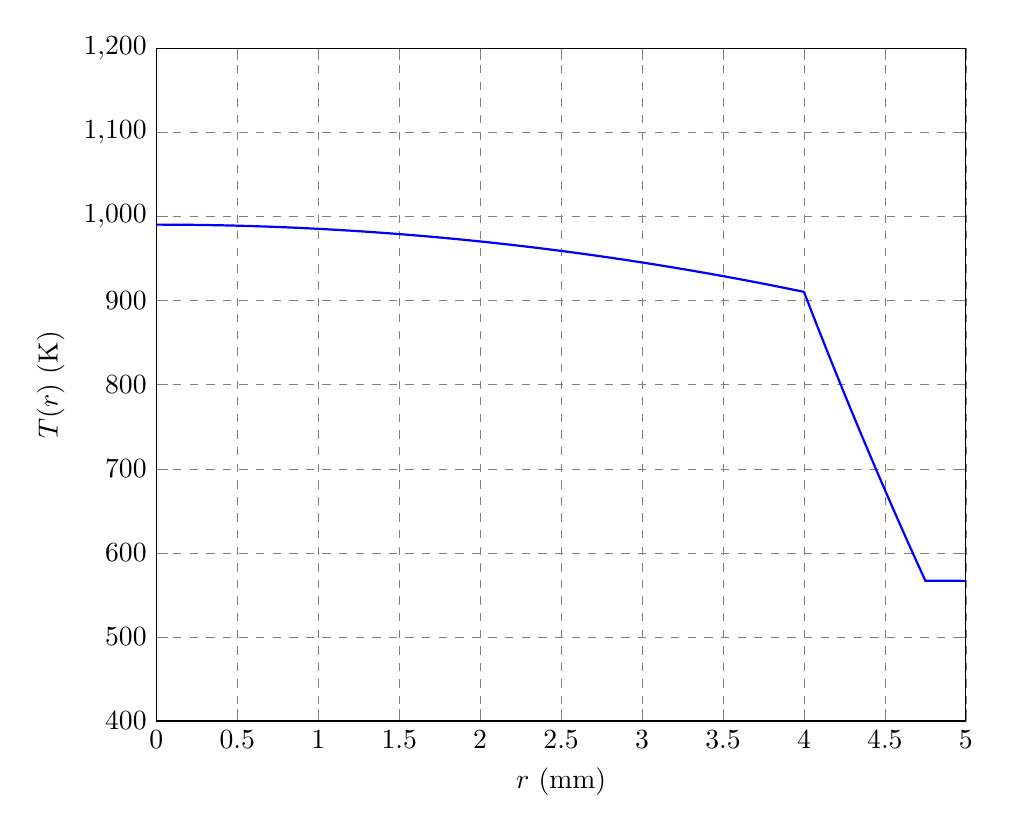
\begin{tikzpicture} \begin{axis}
[scale=1.5,
 xmin=0,    xmax=5,
 ymin=400, ymax=1200,
 grid=major, 
 major grid style={color=gray,line width=0.2pt, dashed},
 xlabel=$r$ (mm),
 ylabel=$T(r)$ (K),
]

\addplot[line width=0.8pt, color=blue] coordinates {
 (           0 ,  9.9047e+02 )
 (  1.0000e-01 ,  9.9042e+02 )
 (  2.0000e-01 ,  9.9027e+02 )
 (  3.0000e-01 ,  9.9002e+02 )
 (  4.0000e-01 ,  9.8967e+02 )
 (  5.0000e-01 ,  9.8922e+02 )
 (  6.0000e-01 ,  9.8867e+02 )
 (  7.0000e-01 ,  9.8802e+02 )
 (  8.0000e-01 ,  9.8727e+02 )
 (  9.0000e-01 ,  9.8642e+02 )
 (  1.0000e+00 ,  9.8547e+02 )
 (  1.1000e+00 ,  9.8442e+02 )
 (  1.2000e+00 ,  9.8327e+02 )
 (  1.3000e+00 ,  9.8202e+02 )
 (  1.4000e+00 ,  9.8067e+02 )
 (  1.5000e+00 ,  9.7922e+02 )
 (  1.6000e+00 ,  9.7767e+02 )
 (  1.7000e+00 ,  9.7602e+02 )
 (  1.8000e+00 ,  9.7427e+02 )
 (  1.9000e+00 ,  9.7242e+02 )
 (  2.0000e+00 ,  9.7047e+02 )
 (  2.1000e+00 ,  9.6842e+02 )
 (  2.2000e+00 ,  9.6627e+02 )
 (  2.3000e+00 ,  9.6402e+02 )
 (  2.4000e+00 ,  9.6167e+02 )
 (  2.5000e+00 ,  9.5922e+02 )
 (  2.6000e+00 ,  9.5667e+02 )
 (  2.7000e+00 ,  9.5402e+02 )
 (  2.8000e+00 ,  9.5127e+02 )
 (  2.9000e+00 ,  9.4842e+02 )
 (  3.0000e+00 ,  9.4547e+02 )
 (  3.1000e+00 ,  9.4242e+02 )
 (  3.2000e+00 ,  9.3927e+02 )
 (  3.3000e+00 ,  9.3602e+02 )
 (  3.4000e+00 ,  9.3267e+02 )
 (  3.5000e+00 ,  9.2922e+02 )
 (  3.6000e+00 ,  9.2567e+02 )
 (  3.7000e+00 ,  9.2202e+02 )
 (  3.8000e+00 ,  9.1827e+02 )
 (  3.9000e+00 ,  9.1442e+02 )
 (  4.0000e+00 ,  9.1047e+02 )
 (  4.0500e+00 ,  8.8562e+02 )
 (  4.1000e+00 ,  8.6108e+02 )
 (  4.1500e+00 ,  8.3684e+02 )
 (  4.2000e+00 ,  8.1289e+02 )
 (  4.2500e+00 ,  7.8922e+02 )
 (  4.3000e+00 ,  7.6583e+02 )
 (  4.3500e+00 ,  7.4271e+02 )
 (  4.4000e+00 ,  7.1985e+02 )
 (  4.4500e+00 ,  6.9725e+02 )
 (  4.5000e+00 ,  6.7490e+02 )
 (  4.5500e+00 ,  6.5280e+02 )
 (  4.6000e+00 ,  6.3095e+02 )
 (  4.6500e+00 ,  6.0932e+02 )
 (  4.7000e+00 ,  5.8793e+02 )
 (  4.7500e+00 ,  5.6677e+02 )
 (  4.8000e+00 ,  5.6675e+02 )
 (  4.8500e+00 ,  5.6673e+02 )
 (  4.9000e+00 ,  5.6671e+02 )
 (  4.9500e+00 ,  5.6669e+02 )
 (  5.0000e+00 ,  5.6667e+02 )
};
\end{axis}
\end{tikzpicture}
\caption{Temperature distribution in nuclear fuel rod.}
 \label{Fig:ode_temperatureDistributionNuclearFuelRod}
\end{center}
\end{figure}

Using the following values:
\begin{align}
  R_1 &= 0.4 \text{ cm}, \nonumber \\
  R_2 &= 0.475 \text{ cm}, \nonumber \\
  R_3 &= 0.5 \text{ cm}, \nonumber \\
  Q_1 &= 5 \times 10^6 \text{ W$\cdot$m$^{-3}$}, \nonumber \\
  k_1 &= 0.25 \text{ W$\cdot$m$^{-1}\cdot$K$^{-1}$}, \nonumber \\
  k_2 &= 0.02 \text{ W$\cdot$m$^{-1}\cdot$K$^{-1}$}, \nonumber \\
  k_3 &= 20 \text{ W$\cdot$m$^{-1}\cdot$K$^{-1}$}, \nonumber \\
  h   &= 30 \text{ W$\cdot$m$^{-2}\cdot$K$^{-1}$}, \nonumber  \\
  T_\infty &= 300 \text{ K}, \nonumber
\end{align}
we solve the linear system and insert the numerical values into the coefficients. The temperature distribution is plotted in Fig.~\ref{Fig:ode_temperatureDistributionNuclearFuelRod}. The inner region has the fuel with a modest thermal conductivity and heat generation. This leads to a parabolic temperature shape with a small change in temperature change across the region. Moving outward, the next region is the gas-filled gap, with no heat generation and low thermal conductivity. Because the heat transfer is minimal in this region, the temperature field drops significantly. Finally, we have the zircaloy cladding, with a high thermal conductivity. Because of this, the temperature change in the clad is small. 

Notice that in the solution that while the temperature field is continuous, its derivatives at the interfaces are not. Recall that the heat flux is continuous across interfaces, which is proportional to the derivative times the thermal conductivity, which varies quite significantly between the fuel, gap, and cladding.


%%%%%%%%%%%%%%%%%%%%%%%%%%%%%%%%%%%%%%%%%%%%%%%%%%%%%%%%%%%%%%%%%%%%%%%%%%%%%%%%%%%%%%%%%%%%%%%%
\subsection{Example: Neutron Diffusion in a Planar Lattice}

\begin{figure}[tb!]
\begin{center}
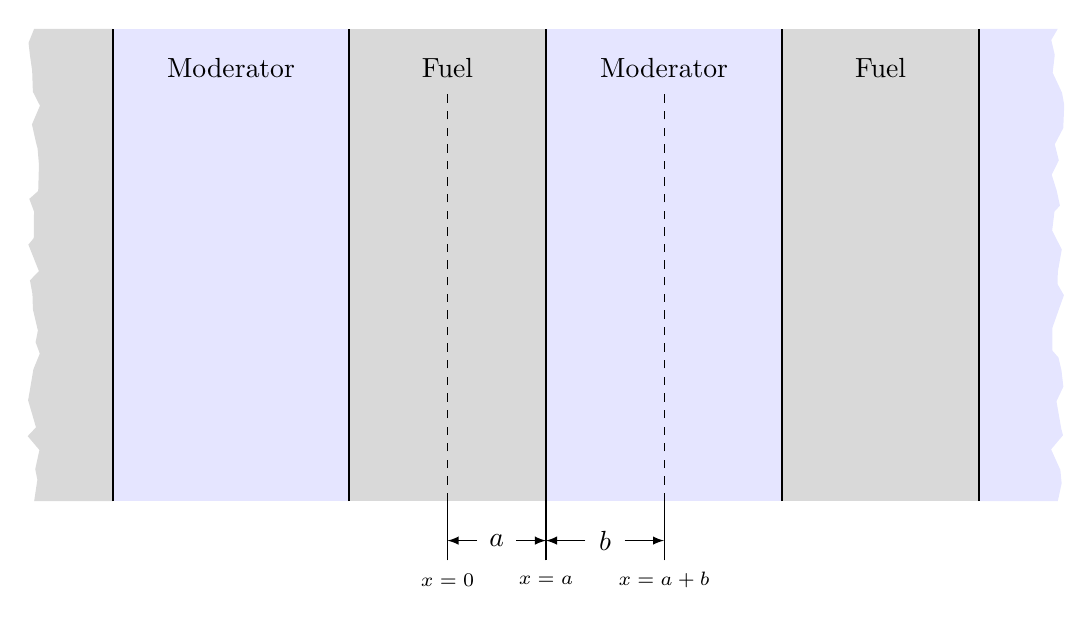
\begin{tikzpicture}
% fuel-moderator boxes
\fill[gray!30, decoration={random steps,segment length=0.2cm}] (-4,-1) decorate{-- (-4,5)} -- (-3,5) -- (-3,-1)-- cycle;
\fill[blue!10] (-3,-1) rectangle (0,5);
\fill[gray!30] (0,-1) rectangle (+2.5,5);
\fill[blue!10] (+2.5,-1) rectangle (+5.5,5);
\fill[gray!30] (+5.5,-1) rectangle (+8.0,5);
\fill[blue!10, decoration={random steps,segment length=0.2cm}] (+9.0,+5.0) decorate{-- (+9.0,-1.0)} -- (+8.0,-1.0) -- (+8.0,+5.0)-- cycle;
%\node at (0,0.5) {\iso{I}{126}{53}};
\draw[thick] (-0,-1) -- (0,5);
\draw[thick] (-3,-1) -- (-3,5);
\draw[thick] (+2.5,-1) -- (+2.5,5);
\draw[thick] (+5.5,-1) -- (+5.5,5);
\draw[thick] (+8.0,-1) -- (+8.0,5);
%
\draw[dashed] (1.25,-1) -- (1.25,4.25);
\draw         (1.25,-1.75) -- (1.25,-1);
\draw         (2.5,-1.75) -- (2.5,-1);
\draw[dashed] (4,-1) -- (4,4.25);
\draw         (4,-1.75) -- (4,-1);
\node at (1.875,-1.5) {$a$};
\draw[-latex] (1.625,-1.5) -- (1.25,-1.5);
\draw[-latex] (2.125,-1.5) -- (2.5,-1.5);
\node at (3.25,-1.5)  {$b$};
\draw[-latex] (3,-1.5) -- (2.5,-1.5);
\draw[-latex] (3.5,-1.5) -- (4,-1.5);
\node at (1.25,-2) {\scriptsize $x = 0$};
\node at (2.5,-2) {\scriptsize $x = a$};
\node at (4,-2) {\scriptsize $x = a+b$};
\node at (-1.5,+4.5) {Moderator};
\node at (+1.25,+4.5) {Fuel};
\node at (+4.0,+4.5) {Moderator};
\node at (+6.75,+4.5) {Fuel};
\end{tikzpicture}
\caption{Illustration of a planar fuel-moderator lattice.}
\label{Fig:ode_planarLattice}
\end{center}
\end{figure}


The theory of neutron diffusion is often used to model the neutron field distribution in nuclear reactor analysis. Neutron diffusion is an approximation to the more accurate model of neutron transport, but tends to work well in situations where the neutrons in the field are not too biased in a particular direction (cf., a particle beam). In this problem we consider the case where we model the spatial distribution of neutrons that have completely slowed down following moderation, i.e. thermal neutrons. The differential equation for neutron diffusion in 1-D Cartesian geometry with a single energy group is
\begin{align}
  -D \frac{d^2 \phi}{dx^2} + \Sigma_a \phi(x) = Q(x).
\end{align}
Here $\phi(x)$ is the scalar flux or path-length rate density of the neutrons (units of neutrons per area per time), $D$ is the neutron diffusion coefficient (units of length), $\Sigma_a$ is the macroscopic absorption cross section (units of per length), and $Q(x)$ is the inhomogeneous neutron source term (units of neutrons per volume per time). We often divide by $-D$ and write this as
\begin{align}
  \frac{d^2 \phi}{dx^2} - \frac{1}{L^2} \phi(x) = -\frac{Q(x)}{D},
\end{align}
where $L$ is called the diffusion length (units of length),
\begin{align}
  L = \sqrt{ \frac{D}{\Sigma_a} }.
\end{align}
We also define the net neutron current, or net flow rate of neutrons as
\begin{align}
  J(x) = -D \frac{d\phi}{dx}.
\end{align}

The problem geometry will be an infinite 1-D planar lattice of fuel and moderator regions with fuel as region 1 and moderator as region 2 (see Fig.~\ref{Fig:ode_planarLattice}) . Since the problem exhibits symmetry we can analyze a single unit cell with symmetry boundary conditions at the reflection planes, namely that the net flow rates of neutrons (neutron current) $J(x)$ are zero across the reflection boundaries. The interface conditions require that both the neutron scalar flux $\phi(x)$ and current $J(x)$ are continuous across the interface. The neutron source will be spatially constant in region 2, which is the moderator and represents where neutrons slow down into the thermal group. The equations for the fuel and moderator are respectively,
\begin{subequations}
\begin{align}
  &\phi_1''(x) - \frac{1}{L_1^2} \phi_1(x) = 0, \quad 0 \le x \le a; \\*
  &\phi_2''(x) - \frac{1}{L_2^2} \phi_2(x) = -\frac{Q}{D_2}, \quad a \le x \le a + b.
\end{align}
\end{subequations}
The boundary and interface conditions are
\begin{subequations}
\begin{align}
  J_1(0) &= 0, \\*
  \phi_1(a) &= \phi_2(a), \\*
  J_1(a) &= J_2(a), \\*
  J_2(a+b) &= 0.
\end{align}
\end{subequations}

The solutions to the differential equations involve real exponentials that we elect to write in terms of the hyperbolic trigonometric functions. This is motivated by the fact that the $\sinh(0) = 0$, which we can use to simplify some of the coefficients. For the moderator region, we also introduce a translation by $a + b$ so we get the $\sinh$ term disappear when we apply the boundary condition. These are
\begin{subequations}
\begin{align}
  \phi_1(x) &= A_1 \sinh \left( \frac{x}{L_1} \right) + B_1 \cosh \left( \frac{x}{L_2} \right), \\*
  \phi_2(x) &= A_2 \sinh \left( \frac{a+b-x}{L_2} \right) + B_2 \cosh \left( \frac{a+b-x}{L_2} \right) + \frac{Q L_2^2}{D_2}.
\end{align}
\end{subequations}
The net currents are
\begin{subequations}
\begin{align}
  J_1(x) &= -\frac{D_1 A_1}{L_1} \cosh \left( \frac{x}{L_1} \right)     - \frac{D_1 B_1}{L_1} \sinh \left( \frac{x}{L_2} \right), \\*
  J_2(x) &=  \frac{D_2 A_2}{L_2} \cosh \left( \frac{a+b-x}{L_2} \right) + \frac{D_2 B_2}{L_2} \sinh \left( \frac{a+b-x}{L_2} \right) .
\end{align}
\end{subequations}
Applying the symmetry conditions $J_1(0) = 0$ and $J_2(a+b) = 0$, gives the equations
\begin{subequations}
\begin{align}
  -\frac{D_1 A_1}{L_1} &= 0, \\*
   \frac{D_2 A_2}{L_2} &= 0,
\end{align}
which implies that $A_1 = A_2 = 0$. Applying the interface conditions, we obtain
\begin{align}
  &B_1 \cosh \left( \frac{a}{L_1} \right) = B_2 \cosh \left( \frac{b}{L_2} \right) + \frac{Q L_2^2}{D_2}, \\*
  &- \frac{D_1 B_1}{L_1} \sinh \left( \frac{a}{L_1} \right) = \frac{D_2 B_2}{L_2} \sinh \left( \frac{b}{L_2} \right) .
\end{align}
\end{subequations}
We can then write these two equations as a linear system in terms of the coefficients
\begin{align}
  \left[ \begin{array}{c c}
  \cosh \left( \dfrac{a}{L_1} \right)                  & - \cosh \left( \dfrac{b}{L_2} \right) \vspace{0.2cm} \\
  \dfrac{D_1}{L_1} \sinh \left( \dfrac{a}{L_1} \right) & \dfrac{D_2}{L_2} \sinh \left( \dfrac{b}{L_2} \right) \\
  \end{array} \right]
  \left[ \begin{array}{c} B_1 \\ B_2 \\ \end{array} \right] =
  \left[ \begin{array}{c} \dfrac{Q L_2^2}{D_2} \vspace{0.2cm} \\ 0 \end{array} \right] .
\end{align}
Solving this system for the coefficients yields
\begin{subequations}
\begin{align}
  B_1 &= \dfrac{Q L_2^2}{D_2} \left[
         \dfrac{ \dfrac{D_2}{L_2} \sinh \left( \dfrac{b}{L_2} \right) }
               { \dfrac{D_2}{L_2} \cosh \left( \dfrac{a}{L_1} \right) \sinh  \left( \dfrac{b}{L_2} \right)
               + \dfrac{D_1}{L_1} \sinh \left( \dfrac{a}{L_1} \right) \cosh  \left( \dfrac{b}{L_2} \right) } \right], \\*
  B_2 &= -\dfrac{Q L_2^2}{D_2} \left[
         \dfrac{ \dfrac{D_1}{L_1} \sinh \left( \dfrac{a}{L_1} \right) }
               { \dfrac{D_2}{L_2} \cosh \left( \dfrac{a}{L_1} \right) \sinh  \left( \dfrac{b}{L_2} \right)
               + \dfrac{D_1}{L_1} \sinh \left( \dfrac{a}{L_1} \right) \cosh  \left( \dfrac{b}{L_2} \right) } \right].
\end{align}
\end{subequations}
Therefore the solution is
\begin{subequations}
\begin{align}
  \phi_1(x) &= \dfrac{Q L_2^2}{D_2} \left[
         \dfrac{ \dfrac{D_2}{L_2} \sinh \left( \dfrac{b}{L_2} \right) \cosh \left( \dfrac{x}{L_2} \right) }
               { \dfrac{D_2}{L_2} \cosh \left( \dfrac{a}{L_1} \right) \sinh  \left( \dfrac{b}{L_2} \right)
               + \dfrac{D_1}{L_1} \sinh \left( \dfrac{a}{L_1} \right) \cosh  \left( \dfrac{b}{L_2} \right) } \right] , \\*
  \phi_2(x) &= \dfrac{Q L_2^2}{D_2} \left[ 1 -
                \dfrac{ \dfrac{D_1}{L_1} \sinh \left( \dfrac{a}{L_1} \right) \cosh \left( \dfrac{a+b-x}{L_2} \right) }
               { \dfrac{D_2}{L_2} \cosh \left( \dfrac{a}{L_1} \right) \sinh  \left( \dfrac{b}{L_2} \right)
               + \dfrac{D_1}{L_1} \sinh \left( \dfrac{a}{L_1} \right) \cosh  \left( \dfrac{b}{L_2} \right) } \right] .
\end{align}
\end{subequations}

\begin{figure}[tb!]
\begin{center}
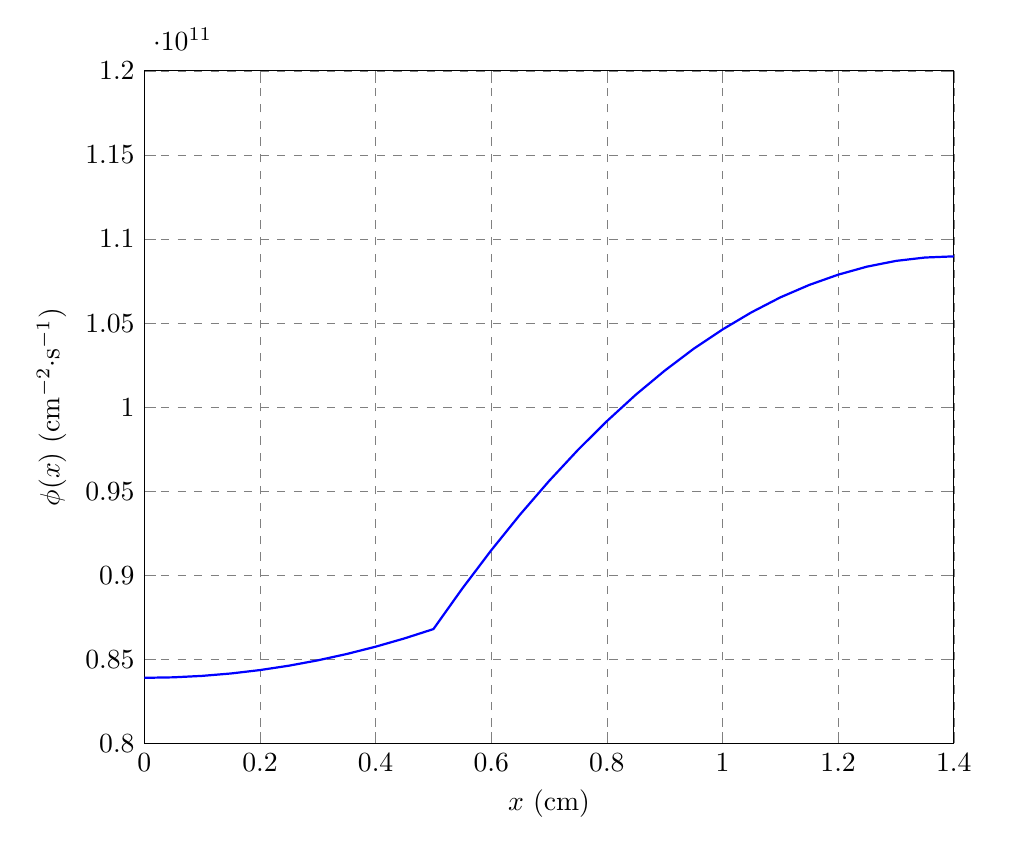
\begin{tikzpicture} \begin{axis}
[scale=1.5,
 xmin=0,    xmax=1.4,
 ymin=8.0e10, ymax=1.2e11,
 grid=major, 
 major grid style={color=gray,line width=0.2pt, dashed},
 xlabel=$x$ (cm),
 ylabel=$\phi(x)$ (cm$^{-2}\cdot$s$^{-1}$),
]

\addplot[line width=0.8pt, color=blue] coordinates {
 (           0 ,  8.3901e+10 )
 (  5.0000e-02 ,  8.3930e+10 )
 (  1.0000e-01 ,  8.4016e+10 )
 (  1.5000e-01 ,  8.4160e+10 )
 (  2.0000e-01 ,  8.4362e+10 )
 (  2.5000e-01 ,  8.4622e+10 )
 (  3.0000e-01 ,  8.4940e+10 )
 (  3.5000e-01 ,  8.5317e+10 )
 (  4.0000e-01 ,  8.5752e+10 )
 (  4.5000e-01 ,  8.6246e+10 )
 (  5.0000e-01 ,  8.6799e+10 )
 (  5.5000e-01 ,  8.9214e+10 )
 (  6.0000e-01 ,  9.1487e+10 )
 (  6.5000e-01 ,  9.3617e+10 )
 (  7.0000e-01 ,  9.5607e+10 )
 (  7.5000e-01 ,  9.7457e+10 )
 (  8.0000e-01 ,  9.9167e+10 )
 (  8.5000e-01 ,  1.0074e+11 )
 (  9.0000e-01 ,  1.0217e+11 )
 (  9.5000e-01 ,  1.0347e+11 )
 (  1.0000e+00 ,  1.0462e+11 )
 (  1.0500e+00 ,  1.0564e+11 )
 (  1.1000e+00 ,  1.0653e+11 )
 (  1.1500e+00 ,  1.0727e+11 )
 (  1.2000e+00 ,  1.0788e+11 )
 (  1.2500e+00 ,  1.0836e+11 )
 (  1.3000e+00 ,  1.0870e+11 )
 (  1.3500e+00 ,  1.0890e+11 )
 (  1.4000e+00 ,  1.0897e+11 )
};
\end{axis}
\end{tikzpicture}
\caption{Neutron scalar flux (path-length rate density) in a planar fuel-moderator lattice.}
 \label{Fig:ode_neutronFluxPlanarLattice}
\end{center}
\end{figure}

The following numbers are representative for a uranium dioxide fuel and light water moderator:
\begin{align}
  a &= 0.5 \text{ cm}, \nonumber \\
  b &= 0.9 \text{ cm}, \nonumber \\
  Q &= 10^{10} \text{ neutrons$\cdot$cm$^{-3}$$\cdot$s$^{-1}$}, \nonumber \\
  D_1 &= 0.615 \text{ cm}, \nonumber \\
  D_2 &= 0.144 \text{ cm}, \nonumber \\
  L_1 &= 1.908 \text{ cm}, \nonumber \\
  L_2 &= 2.685 \text{ cm}. \nonumber
\end{align}
Using those numbers the scalar flux is plotted in Fig.~\ref{Fig:ode_neutronFluxPlanarLattice}. The thermal neutron scalar flux is highest in the moderator region on the right, as this is where the neutrons thermalize. The scalar flux falls as the field gets closer to the fuel as neutrons that enter the fuel tend to be absorbed (some of these absorptions cause fission) and therefore fewer neutrons exit the fuel than exit. As one may expect, the minimum neutron scalar flux is at the center of the fuel.


%%%%%%%%%%%%%%%%%%%%%%%%%%%%%%%%%%%%%%%%%%%%%%%%%%%%%%%%%%%%%%%%%%%%%%%%%%%%%%%%%%%%%%%%%%%%%%%%
\subsection{Example: Quantum Particle in a Finite Potential Well}

\begin{figure}[tb!]
\begin{center}
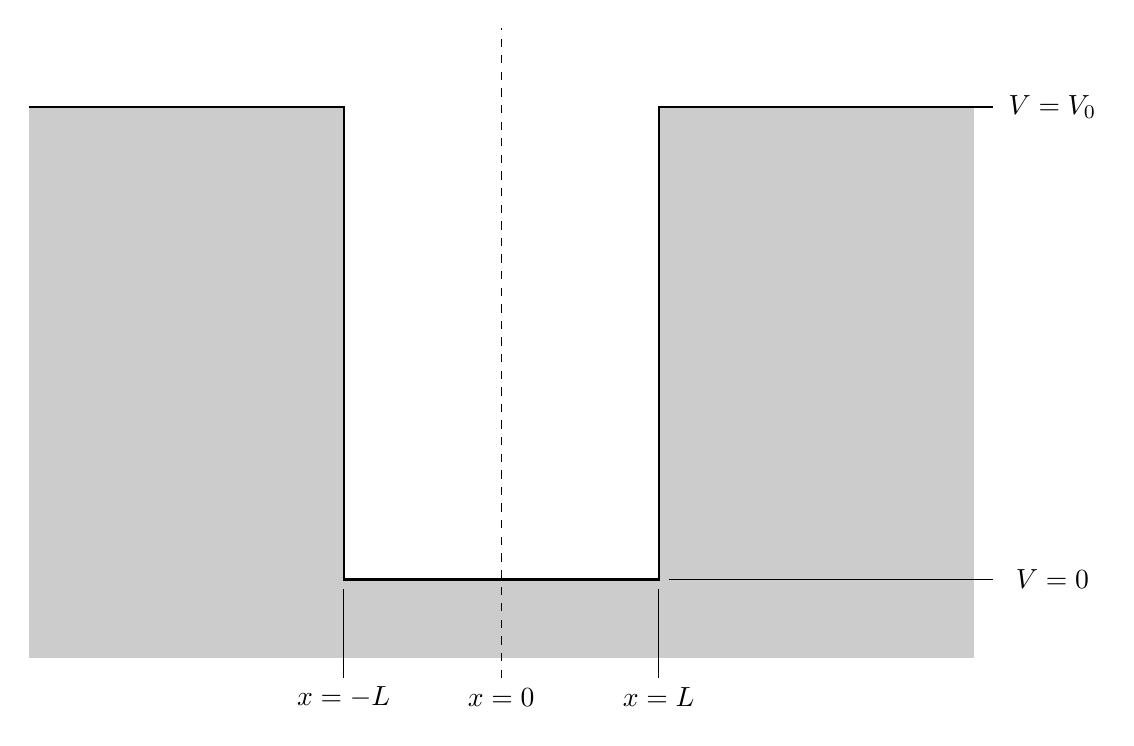
\begin{tikzpicture}
  \fill[gray!40] (-6,-1) -- (-2,-1) -- (-2,6) -- (-6,6);
  \fill[gray!40] (-2,-1) -- ( 2,-1) -- ( 2,0) -- (-2,0);
  \fill[gray!40] ( 2,-1) -- ( 6,-1) -- ( 6,6) -- ( 2,6);
  \draw[thick] (-6,6) -- (-2,6) -- (-2,0) -- (2,0) -- (2,6) -- (6,6);
  \draw[dashed] (0,-1.25) -- (0,7);
  \node at (0,-1.5) {$x = 0$};
  \draw (-2,-0.125) -- (-2,-1.25);
  \node at (-2,-1.5) {$x = -L$};
  \draw (2,-0.125) -- (2,-1.25);
  \node at (2,-1.5) {$x = L$};
  \draw (2.125,0) -- (6.25,0);
  \node at (7,0) {$V = 0$};
  \draw (2.125,6) -- (6.25,6);
  \node at (7,6) {$V = V_0$};
\end{tikzpicture}
\caption{Illustration of a finite potential (square) well.}
\label{Fig:ode_finitePotentialWell}
\end{center}
\end{figure}

In quantum mechanics, particles are described by wavefunctions using the Schr{\"o}dinger equation. The steady-state, 1-D Cartesian form is
\begin{align}
  -\frac{\hbar^2}{2m} \frac{d^2\psi}{dx^2} + V(x) \psi(x) = E \psi(x).
\end{align}
Here $\psi(x)$ is the wavefunction of the particle, $\hbar = h/(2\pi)$ or the reduced Planck's constant, $m$ is the mass of the particle, $V(x)$ is a prescribed potential energy field, and $E$ is the energy of the particle. The wavefunction $\psi(x)$ is generally a complex function that is related to the probability of a particle being at a certain point in space. The probability per unit length (probability density) is given by
\begin{align} 
  f(x) = \psi(x) \psi^*(x),
\end{align}
where $\psi^*(x)$ is the complex conjugate of $\psi(x)$. Because of the nature of probabilities, the wavefunction has the normalization
\begin{align}
  \int_{-\infty}^\infty \psi(x) \psi^*(x) dx = 1.
\end{align}
The wavefunction and its first derivative must be continuous at interfaces and must be finite everywhere.

Here we consider the case of a symmetric finite potential well with width $2L$ (see Fig.~\ref{Fig:ode_finitePotentialWell}) with the potential function
\begin{align}
  V(x) = \left\{ \begin{array}{l c} V_0 & x < -L \\ 0 & -L \le x \le L \\ V_0 & x > L \end{array} \right. .
\end{align}
Because of symmetry we can simplify this problem and only solve the right half of the problem $x \ge 0$ with region 1 being $0 \le x \le L$ and region 2 being $x > L$.  The differential equations become
\begin{subequations}
\begin{align}
  &\frac{d^2 \psi_1}{dx^2} + \frac{2mE}{\hbar^2} \psi_1(x) = 0, \\*
  &\frac{d^2 \psi_2}{dx^2} - \frac{2m(V_0 - E)}{\hbar^2} \psi_2(x) = 0.
\end{align}
\end{subequations}
As we can see from the second equation, that we will get different behavior if $E < V_0$ and $E > V_0$. Since the case with $E < V_0$ is more interesting, let us consider that case. For this, we define the following coefficients:
\begin{subequations}
\begin{align}
  &k_1^2 = \frac{2mE}{\hbar^2}, \\*
  &k_2^2 = \frac{2m(V_0 - E)}{\hbar^2}.
\end{align}
\end{subequations}
The equations are therefore
\begin{subequations}
\begin{align}
  &\frac{d^2 \psi_1}{dx^2} + k_1^2 \psi_1(x) = 0, \\*
  &\frac{d^2 \psi_2}{dx^2} - k_2^2 \psi_2(x) = 0, 
\end{align}
\end{subequations}
which have the solutions
\begin{subequations}
\begin{align}
  \psi_1(x) &= A_1 \sin ( k_1 x ) + B_1 \cos ( k_1 x ), \\
  \psi_2(x) &= A_2 e^{k_2 x} + B_2 e^{-k_2 x} .
\end{align}
\end{subequations}
Since we require that the wavefunction be finite everywhere, we require that $A_2 = 0$. Therefore,
\begin{subequations}
\begin{align}
  \psi_1(x) &= A_1 \sin ( k_1 x ) + B_1 \cos ( k_1 x ), \\*
  \psi_2(x) &= B_2 e^{-k_2 x} .
\end{align}
\end{subequations}
The derivatives are
\begin{subequations}
\begin{align}
  \frac{d\psi_1}{dx} &= A_1 k_1 \cos ( k_1 x ) - B_1 k_1 \sin ( k_1 x ), \\*
  \frac{d\psi_2}{dx} &= -B_2 k_2 e^{-k_2 x} .
\end{align}
\end{subequations}

To help with the boundary and interface conditions, we make an observation that there are two types of symmetry that the wavefunction may possess. First, the wavefunction may be reflected about the $y$-axis, which are the \emph{even parity} solutions denoted by $\psi^+(x)$. Second, since the wavefunction may be both positive and negative, we must also permit \emph{odd parity} solutions reflected about the origin, which we denote by $\psi^-(x)$. Because the Schr{\"o}dinger equation is linear, we can apply the superposition principle and solve for the even and odd solutions separately and then add them together,
\begin{align}
  \psi(x) = \psi^+(x) + \psi^-(x).
\end{align}

The even parity solutions must be reflected about the $y$-axis and since its derivative must be smooth, we demand that
\begin{subequations}
\begin{align}
  \frac{d\psi_1^+}{dx} \bigg|_{x=0} = 0. 
\end{align}
For the odd-parity solutions, we require symmetry with respect to the origin so we enforce that
\begin{align}
  \psi_1^-(0) = 0.
\end{align}
Both the even and odd parity solutions and their respective first derivatives must be continuous across the interface at $x = L$:
\begin{align}
  \psi_1^\pm(L) &= \psi_2^\pm(L), \\*
  \frac{d\psi_1^\pm}{dx} \bigg|_{x=L} &= \frac{d\psi_2^\pm}{dx} \bigg|_{x=L}
\end{align}
\end{subequations}

Let us begin by solving for the even parity wavefunction. Applying the boundary condition that the first-derivative at $x = 0$ is zero, gives
\begin{align}
  A_1 k_1 = 0,
\end{align}
meaning that $A_1 = 0$. The interface conditions are therefore
\begin{subequations}
\begin{align}
  B_1 \cos ( k_1 L ) &= B_2 e^{-k_2 L}, \\*
  - B_1 k_1 \sin ( k_1 L ) &= -B_2 k_2 e^{-k_2 L} .
\end{align}
\end{subequations}
This yields the following linear system:
\begin{align}
  \left[ \begin{array}{c c}
       \cos( k_1 L ) &     -e^{-k_2 L} \\
  -k_1 \sin( k_1 L ) &  k_2 e^{-k_2 L} \\ \end{array} \right]
  \left[ \begin{array}{c} B_1 \\ B_2 \\ \end{array} \right] =
  \left[ \begin{array}{c} 0 \\ 0 \\ \end{array} \right] .
\end{align}
For this system to have a solution, either the solution vector must be zero or the determinant of the matrix must be zero. The former case is of no interest, because it describes the case where there is no particle. The latter case yields the following determinant:
\begin{align}
  \left| \begin{array}{c c}
       \cos( k_1 L ) &     -e^{-k_2 L} \\
  -k_1 \sin( k_1 L ) &  k_2 e^{-k_2 L} \\ \end{array} \right| = k_2  e^{-k_2 L} \cos( k_1 L ) - k_1 e^{-k_2 L} \sin( k_1 L ) = 0.
\end{align}
We obtain the relationship:
\begin{align}
  \frac{k_2}{k_1} - \tan ( k_1 L ) = 0.
\end{align}
Unfortunately, this equation cannot be solved directly and solutions must be obtained from an iterative root finding algorithm. 

Repeating this process for the odd parity wavefunction, we apply the boundary condition requiring the wavefunction to go to zero at $x = 0$ yielding
\begin{align}
  B_1 = 0.
\end{align}
The interface conditions are then
\begin{subequations}
\begin{align}
      A_1 \sin ( k_1 L ) &=  B_2 e^{-k_2 L}, \\*
  A_1 k_1 \cos ( k_1 L ) &= -B_2 k_2 e^{-k_2 L} ,
\end{align}
\end{subequations}
which has the linear system
\begin{align}
  \left[ \begin{array}{c c}
       \sin( k_1 L ) &     -e^{-k_2 L} \\
   k_1 \cos( k_1 L ) &  k_2 e^{-k_2 L} \\ \end{array} \right]
  \left[ \begin{array}{c} A_1 \\ B_2 \\ \end{array} \right] =
  \left[ \begin{array}{c} 0 \\ 0 \\ \end{array} \right] .
\end{align}
As before, we find where the determinant is zero,
\begin{align}
  \left| \begin{array}{c c}
       \sin( k_1 L ) &     -e^{-k_2 L} \\
   k_1 \cos( k_1 L ) &  k_2 e^{-k_2 L} \\ \end{array} \right| = k_2  e^{-k_2 L} \sin( k_1 L ) + k_1 e^{-k_2 L} \cos( k_1 L ) = 0.
\end{align}
This gives the solution
\begin{align}
  \frac{k_2}{k_1} + \cot ( k_1 L ) = 0,
\end{align}
which also must be solved numerically.

Putting the resulting transcendental expressions in terms of energy gives
\begin{subequations}
\begin{align}
  g_1(E) &= \sqrt{ \frac{V_0 - E}{E} } - \tan \left( \frac{\sqrt{2mE}L}{\hbar} \right) = 0, \\*
  g_2(E) &= \sqrt{ \frac{V_0 - E}{E} } + \cot \left( \frac{\sqrt{2mE}L}{\hbar} \right) = 0.
\end{align}
\end{subequations}
At this point, let us introduce some numerical values corresponding to an electron in a 20~eV potential well with a width of 0.4~nm:
\begin{align}
  \hbar &= 1.055 \times 10^{-34} \text{ J$\cdot$s}, \nonumber \\*
      m &= 9.109 \times 10^{-31} \text{ kg}, \nonumber \\*
      L &= 2 \times 10^{-10} \text{ m}, \nonumber \\*
    V_0 &= 20 \text{ eV} = 3.204 \times 10^{-18} \text{ J}. \nonumber
\end{align}

\begin{figure}[tb!]
\begin{center}
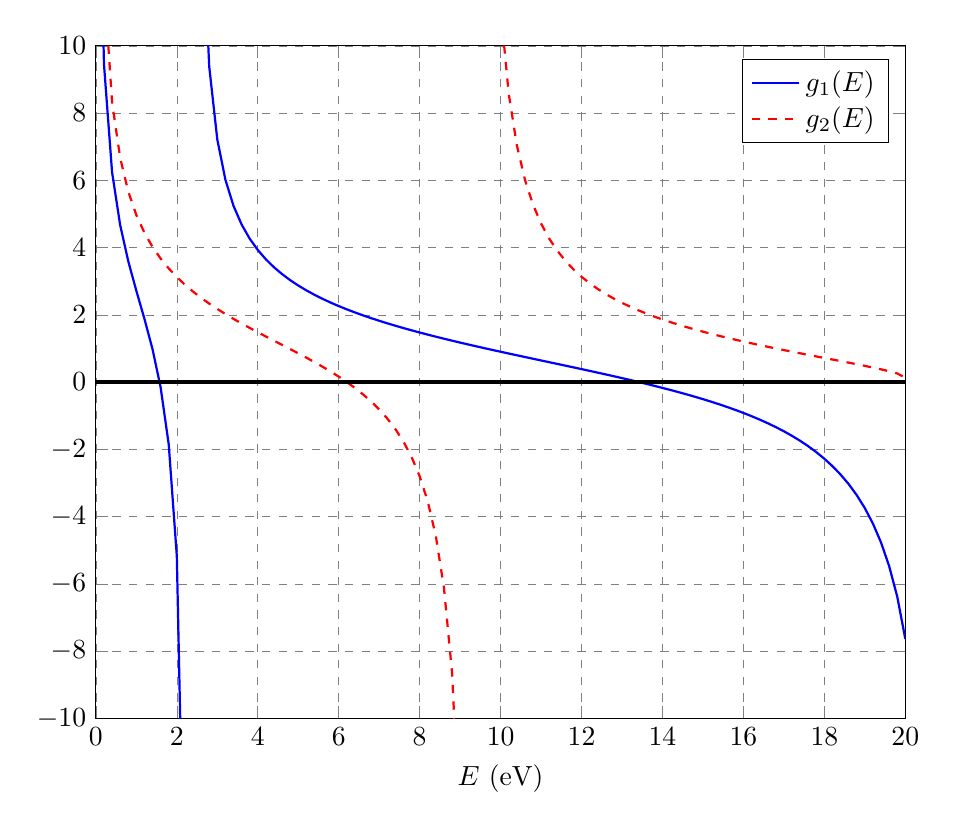
\begin{tikzpicture} \begin{axis}
[scale=1.5,
 xmin=0,    xmax=20,
 ymin=-10, ymax=10,
 grid=major, 
 major grid style={color=gray,line width=0.2pt, dashed},
 xlabel=$E$ (eV),
]

\addplot[line width=0.8pt, color=blue] coordinates {
  ( 0          ,  20 )
  ( 2.0000e-01 ,  9.4566e+00 )
  ( 4.0000e-01 ,  6.2429e+00 )
  ( 6.0000e-01 ,  4.6695e+00 )
  ( 8.0000e-01 ,  3.5953e+00 )
  ( 1.0000e+00 ,  2.7137e+00 )
  ( 1.2000e+00 ,  1.8793e+00 )
  ( 1.4000e+00 ,  9.7559e-01 )
  ( 1.6000e+00 , -1.5673e-01 )
  ( 1.8000e+00 , -1.8538e+00 )
  ( 2.0000e+00 , -5.1729e+00 )
  ( 2.2000e+00 , -1.6737e+01 )
};

\addplot[line width=0.8pt, color=red, dashed] coordinates {
 (  2.0000e-01 ,  1.1977e+01 )
 (  4.0000e-01 ,  8.3208e+00 )
 (  6.0000e-01 ,  6.6698e+00 )
 (  8.0000e-01 ,  5.6661e+00 )
 (  1.0000e+00 ,  4.9667e+00 )
 (  1.2000e+00 ,  4.4392e+00 )
 (  1.4000e+00 ,  4.0196e+00 )
 (  1.6000e+00 ,  3.6730e+00 )
 (  1.8000e+00 ,  3.3785e+00 )
 (  2.0000e+00 ,  3.1224e+00 )
 (  2.2000e+00 ,  2.8955e+00 )
 (  2.4000e+00 ,  2.6915e+00 )
 (  2.6000e+00 ,  2.5054e+00 )
 (  2.8000e+00 ,  2.3337e+00 )
 (  3.0000e+00 ,  2.1737e+00 )
 (  3.2000e+00 ,  2.0230e+00 )
 (  3.4000e+00 ,  1.8798e+00 )
 (  3.6000e+00 ,  1.7427e+00 )
 (  3.8000e+00 ,  1.6103e+00 )
 (  4.0000e+00 ,  1.4813e+00 )
 (  4.2000e+00 ,  1.3549e+00 )
 (  4.4000e+00 ,  1.2299e+00 )
 (  4.6000e+00 ,  1.1055e+00 )
 (  4.8000e+00 ,  9.8064e-01 )
 (  5.0000e+00 ,  8.5437e-01 )
 (  5.2000e+00 ,  7.2566e-01 )
 (  5.4000e+00 ,  5.9336e-01 )
 (  5.6000e+00 ,  4.5619e-01 )
 (  5.8000e+00 ,  3.1268e-01 )
 (  6.0000e+00 ,  1.6109e-01 )
 (  6.2000e+00 , -6.9681e-04 )
 (  6.4000e+00 , -1.7528e-01 )
 (  6.6000e+00 , -3.6594e-01 )
 (  6.8000e+00 , -5.7692e-01 )
 (  7.0000e+00 , -8.1380e-01 )
 (  7.2000e+00 , -1.0841e+00 )
 (  7.4000e+00 , -1.3985e+00 )
 (  7.6000e+00 , -1.7721e+00 )
 (  7.8000e+00 , -2.2275e+00 )
 (  8.0000e+00 , -2.8005e+00 )
 (  8.2000e+00 , -3.5504e+00 )
 (  8.4000e+00 , -4.5837e+00 )
 (  8.6000e+00 , -6.1136e+00 )
 (  8.8000e+00 , -8.6371e+00 )
 (  9.0000e+00 , -1.3642e+01 )
 (  9.2000e+00 , -2.8548e+01 )
};

\addplot[line width=0.8pt, color=blue] coordinates {
  ( 2.4000e+00 ,  6.3111e+01 )
  ( 2.6000e+00 ,  1.4849e+01 )
  ( 2.8000e+00 ,  9.3876e+00 )
  ( 3.0000e+00 ,  7.2163e+00 )
  ( 3.2000e+00 ,  6.0186e+00 )
  ( 3.4000e+00 ,  5.2421e+00 )
  ( 3.6000e+00 ,  4.6876e+00 )
  ( 3.8000e+00 ,  4.2650e+00 )
  ( 4.0000e+00 ,  3.9280e+00 )
  ( 4.2000e+00 ,  3.6499e+00 )
  ( 4.4000e+00 ,  3.4143e+00 )
  ( 4.6000e+00 ,  3.2105e+00 )
  ( 4.8000e+00 ,  3.0313e+00 )
  ( 5.0000e+00 ,  2.8714e+00 )
  ( 5.2000e+00 ,  2.7272e+00 )
  ( 5.4000e+00 ,  2.5958e+00 )
  ( 5.6000e+00 ,  2.4751e+00 )
  ( 5.8000e+00 ,  2.3634e+00 )
  ( 6.0000e+00 ,  2.2594e+00 )
  ( 6.2000e+00 ,  2.1619e+00 )
  ( 6.4000e+00 ,  2.0701e+00 )
  ( 6.6000e+00 ,  1.9833e+00 )
  ( 6.8000e+00 ,  1.9008e+00 )
  ( 7.0000e+00 ,  1.8222e+00 )
  ( 7.2000e+00 ,  1.7470e+00 )
  ( 7.4000e+00 ,  1.6748e+00 )
  ( 7.6000e+00 ,  1.6053e+00 )
  ( 7.8000e+00 ,  1.5381e+00 )
  ( 8.0000e+00 ,  1.4732e+00 )
  ( 8.2000e+00 ,  1.4101e+00 )
  ( 8.4000e+00 ,  1.3488e+00 )
  ( 8.6000e+00 ,  1.2890e+00 )
  ( 8.8000e+00 ,  1.2306e+00 )
  ( 9.0000e+00 ,  1.1733e+00 )
  ( 9.2000e+00 ,  1.1172e+00 )
  ( 9.4000e+00 ,  1.0620e+00 )
  ( 9.6000e+00 ,  1.0077e+00 )
  ( 9.8000e+00 ,  9.5410e-01 )
  ( 1.0000e+01 ,  9.0111e-01 )
  ( 1.0200e+01 ,  8.4863e-01 )
  ( 1.0400e+01 ,  7.9658e-01 )
  ( 1.0600e+01 ,  7.4485e-01 )
  ( 1.0800e+01 ,  6.9336e-01 )
  ( 1.1000e+01 ,  6.4202e-01 )
  ( 1.1200e+01 ,  5.9074e-01 )
  ( 1.1400e+01 ,  5.3943e-01 )
  ( 1.1600e+01 ,  4.8800e-01 )
  ( 1.1800e+01 ,  4.3637e-01 )
  ( 1.2000e+01 ,  3.8444e-01 )
  ( 1.2200e+01 ,  3.3212e-01 )
  ( 1.2400e+01 ,  2.7931e-01 )
  ( 1.2600e+01 ,  2.2590e-01 )
  ( 1.2800e+01 ,  1.7180e-01 )
  ( 1.3000e+01 ,  1.1688e-01 )
  ( 1.3200e+01 ,  6.1036e-02 )
  ( 1.3400e+01 ,  4.1264e-03 )
  ( 1.3600e+01 , -5.3985e-02 )
  ( 1.3800e+01 , -1.1345e-01 )
  ( 1.4000e+01 , -1.7443e-01 )
  ( 1.4200e+01 , -2.3710e-01 )
  ( 1.4400e+01 , -3.0167e-01 )
  ( 1.4600e+01 , -3.6835e-01 )
  ( 1.4800e+01 , -4.3738e-01 )
  ( 1.5000e+01 , -5.0904e-01 )
  ( 1.5200e+01 , -5.8364e-01 )
  ( 1.5400e+01 , -6.6152e-01 )
  ( 1.5600e+01 , -7.4307e-01 )
  ( 1.5800e+01 , -8.2875e-01 )
  ( 1.6000e+01 , -9.1906e-01 )
  ( 1.6200e+01 , -1.0146e+00 )
  ( 1.6400e+01 , -1.1161e+00 )
  ( 1.6600e+01 , -1.2243e+00 )
  ( 1.6800e+01 , -1.3402e+00 )
  ( 1.7000e+01 , -1.4650e+00 )
  ( 1.7200e+01 , -1.6000e+00 )
  ( 1.7400e+01 , -1.7469e+00 )
  ( 1.7600e+01 , -1.9077e+00 )
  ( 1.7800e+01 , -2.0849e+00 )
  ( 1.8000e+01 , -2.2817e+00 )
  ( 1.8200e+01 , -2.5020e+00 )
  ( 1.8400e+01 , -2.7511e+00 )
  ( 1.8600e+01 , -3.0357e+00 )
  ( 1.8800e+01 , -3.3649e+00 )
  ( 1.9000e+01 , -3.7511e+00 )
  ( 1.9200e+01 , -4.2121e+00 )
  ( 1.9400e+01 , -4.7735e+00 )
  ( 1.9600e+01 , -5.4750e+00 )
  ( 1.9800e+01 , -6.3812e+00 )
  ( 2.0000e+01 , -7.6428e+00 )
};
\addlegendentry{$g_1(E)$};

\addplot[line width=0.8pt, color=red, dashed] coordinates {
 (  9.6000e+00 ,  3.1234e+01 )
 (  9.8000e+00 ,  1.6148e+01 )
 (  1.0000e+01 ,  1.1112e+01 )
 (  1.0200e+01 ,  8.5810e+00 )
 (  1.0400e+01 ,  7.0512e+00 )
 (  1.0600e+01 ,  6.0218e+00 )
 (  1.0800e+01 ,  5.2784e+00 )
 (  1.1000e+01 ,  4.7139e+00 )
 (  1.1200e+01 ,  4.2686e+00 )
 (  1.1400e+01 ,  3.9069e+00 )
 (  1.1600e+01 ,  3.6061e+00 )
 (  1.1800e+01 ,  3.3510e+00 )
 (  1.2000e+01 ,  3.1310e+00 )
 (  1.2200e+01 ,  2.9388e+00 )
 (  1.2400e+01 ,  2.7687e+00 )
 (  1.2600e+01 ,  2.6167e+00 )
 (  1.2800e+01 ,  2.4795e+00 )
 (  1.3000e+01 ,  2.3548e+00 )
 (  1.3200e+01 ,  2.2405e+00 )
 (  1.3400e+01 ,  2.1351e+00 )
 (  1.3600e+01 ,  2.0374e+00 )
 (  1.3800e+01 ,  1.9462e+00 )
 (  1.4000e+01 ,  1.8608e+00 )
 (  1.4200e+01 ,  1.7804e+00 )
 (  1.4400e+01 ,  1.7044e+00 )
 (  1.4600e+01 ,  1.6322e+00 )
 (  1.4800e+01 ,  1.5635e+00 )
 (  1.5000e+01 ,  1.4978e+00 )
 (  1.5200e+01 ,  1.4349e+00 )
 (  1.5400e+01 ,  1.3743e+00 )
 (  1.5600e+01 ,  1.3159e+00 )
 (  1.5800e+01 ,  1.2594e+00 )
 (  1.6000e+01 ,  1.2047e+00 )
 (  1.6200e+01 ,  1.1515e+00 )
 (  1.6400e+01 ,  1.0996e+00 )
 (  1.6600e+01 ,  1.0489e+00 )
 (  1.6800e+01 ,  9.9929e-01 )
 (  1.7000e+01 ,  9.5056e-01 )
 (  1.7200e+01 ,  9.0260e-01 )
 (  1.7400e+01 ,  8.5528e-01 )
 (  1.7600e+01 ,  8.0846e-01 )
 (  1.7800e+01 ,  7.6200e-01 )
 (  1.8000e+01 ,  7.1574e-01 )
 (  1.8200e+01 ,  6.6954e-01 )
 (  1.8400e+01 ,  6.2319e-01 )
 (  1.8600e+01 ,  5.7646e-01 )
 (  1.8800e+01 ,  5.2908e-01 )
 (  1.9000e+01 ,  4.8064e-01 )
 (  1.9200e+01 ,  4.3056e-01 )
 (  1.9400e+01 ,  3.7791e-01 )
 (  1.9600e+01 ,  3.2086e-01 )
 (  1.9800e+01 ,  2.5478e-01 )
 (  2.0000e+01 ,  1.3084e-01 )
};
\addlegendentry{$g_2(E)$};

\addplot[line width=1.2pt, color=black] coordinates {
  (0,0)
  (20,0)
};

\end{axis}
\end{tikzpicture}
\caption{Plot of transcendental equations for finite potential well.}
 \label{Fig:ode_finitePotentialWell_transcendentalEquations}
\end{center}
\end{figure}

The functions $g_1(E)$ and $g_2(E)$ are plotted in the domain $0 \le E \le V_0$ in Fig.~\ref{Fig:ode_finitePotentialWell_transcendentalEquations}. As we can see from the plot the even (symmetric) case with the solid blue line cross the $x$-axis twice and the odd (antisymmetric) case with the dashed red line crosses the $x$-axis once. The roots of these functions correspond to the discrete (or quantized) energy states that satisfy the Schr{\"o}dinger equation and its associated boundary conditions. Using a numerical root finder such as Newton-Raphson, the resulting energies are
\begin{align}
  E_1 = 1.58 \text{ eV}, \quad E_2 = 6.20 \text{ eV}, \quad E_3 = 13.41 \text{ eV}. \nonumber
\end{align}
These are the eigenvalues of the Schr{\"o}dinger equation corresponding to this boundary value problem.

\begin{figure}[b!]
\begin{center}
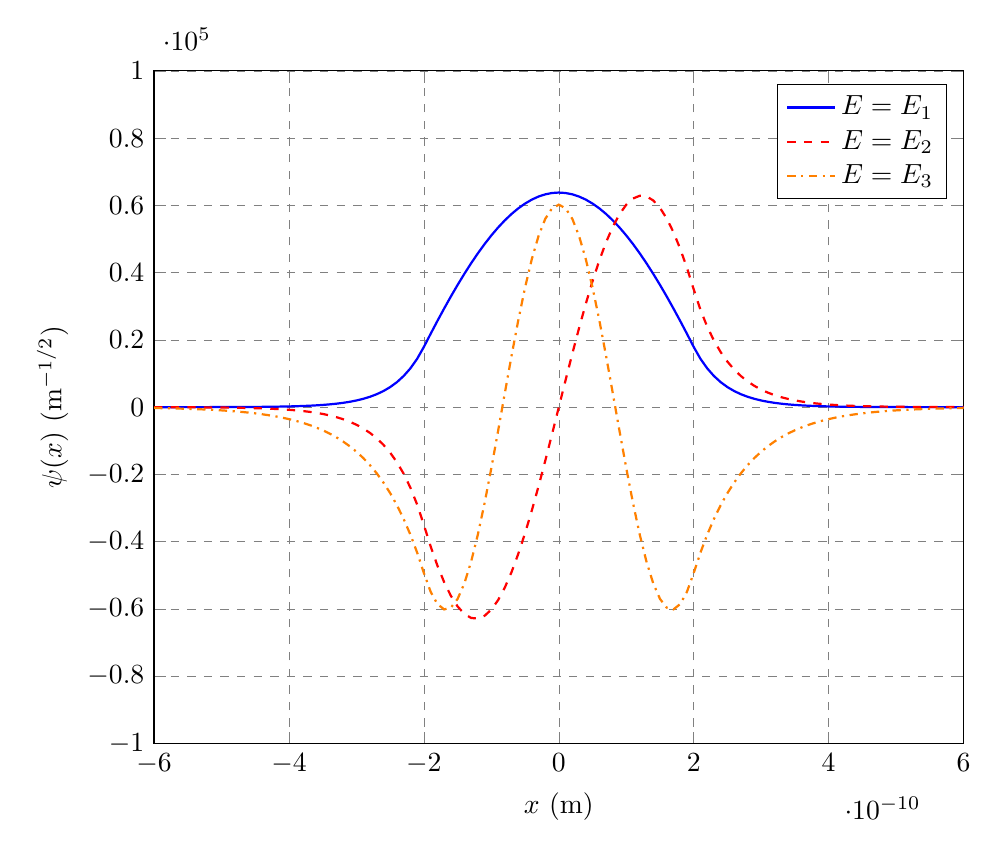
\begin{tikzpicture} \begin{axis}
[scale=1.5,
 xmin=-6e-10,    xmax=6e-10,
 ymin=-1e5, ymax=1e5,
 grid=major, 
 major grid style={color=gray,line width=0.2pt, dashed},
 xlabel=$x$ (m),
 ylabel=$\psi(x)$ (m$^{-1/2}$)
]

\addplot[line width=0.8pt, color=blue] coordinates {
(  -6.0000e-10 ,  2.7111e+00 )
(  -5.9000e-10 ,  3.3779e+00 )
(  -5.8000e-10 ,  4.2087e+00 )
(  -5.7000e-10 ,  5.2439e+00 )
(  -5.6000e-10 ,  6.5337e+00 )
(  -5.5000e-10 ,  8.1407e+00 )
(  -5.4000e-10 ,  1.0143e+01 )
(  -5.3000e-10 ,  1.2638e+01 )
(  -5.2000e-10 ,  1.5746e+01 )
(  -5.1000e-10 ,  1.9619e+01 )
(  -5.0000e-10 ,  2.4444e+01 )
(  -4.9000e-10 ,  3.0456e+01 )
(  -4.8000e-10 ,  3.7947e+01 )
(  -4.7000e-10 ,  4.7280e+01 )
(  -4.6000e-10 ,  5.8909e+01 )
(  -4.5000e-10 ,  7.3398e+01 )
(  -4.4000e-10 ,  9.1451e+01 )
(  -4.3000e-10 ,  1.1394e+02 )
(  -4.2000e-10 ,  1.4197e+02 )
(  -4.1000e-10 ,  1.7689e+02 )
(  -4.0000e-10 ,  2.2039e+02 )
(  -3.9000e-10 ,  2.7460e+02 )
(  -3.8000e-10 ,  3.4214e+02 )
(  -3.7000e-10 ,  4.2629e+02 )
(  -3.6000e-10 ,  5.3114e+02 )
(  -3.5000e-10 ,  6.6177e+02 )
(  -3.4000e-10 ,  8.2454e+02 )
(  -3.3000e-10 ,  1.0273e+03 )
(  -3.2000e-10 ,  1.2800e+03 )
(  -3.1000e-10 ,  1.5948e+03 )
(  -3.0000e-10 ,  1.9871e+03 )
(  -2.9000e-10 ,  2.4758e+03 )
(  -2.8000e-10 ,  3.0848e+03 )
(  -2.7000e-10 ,  3.8435e+03 )
(  -2.6000e-10 ,  4.7889e+03 )
(  -2.5000e-10 ,  5.9667e+03 )
(  -2.4000e-10 ,  7.4342e+03 )
(  -2.3000e-10 ,  9.2627e+03 )
(  -2.2000e-10 ,  1.1541e+04 )
(  -2.1000e-10 ,  1.4380e+04 )
(  -2.0000e-10 ,  1.7916e+04 )
(  -2.0000e-10 ,  1.7916e+04 )
(  -1.9000e-10 ,  2.1816e+04 )
(  -1.8000e-10 ,  2.5626e+04 )
(  -1.7000e-10 ,  2.9330e+04 )
(  -1.6000e-10 ,  3.2913e+04 )
(  -1.5000e-10 ,  3.6359e+04 )
(  -1.4000e-10 ,  3.9655e+04 )
(  -1.3000e-10 ,  4.2788e+04 )
(  -1.2000e-10 ,  4.5743e+04 )
(  -1.1000e-10 ,  4.8509e+04 )
(  -1.0000e-10 ,  5.1075e+04 )
(  -9.0000e-11 ,  5.3429e+04 )
(  -8.0000e-11 ,  5.5563e+04 )
(  -7.0000e-11 ,  5.7466e+04 )
(  -6.0000e-11 ,  5.9133e+04 )
(  -5.0000e-11 ,  6.0554e+04 )
(  -4.0000e-11 ,  6.1726e+04 )
(  -3.0000e-11 ,  6.2642e+04 )
(  -2.0000e-11 ,  6.3299e+04 )
(  -1.0000e-11 ,  6.3694e+04 )
(            0 ,  6.3826e+04 )
(   1.0000e-11 ,  6.3694e+04 )
(   2.0000e-11 ,  6.3299e+04 )
(   3.0000e-11 ,  6.2642e+04 )
(   4.0000e-11 ,  6.1726e+04 )
(   5.0000e-11 ,  6.0554e+04 )
(   6.0000e-11 ,  5.9133e+04 )
(   7.0000e-11 ,  5.7466e+04 )
(   8.0000e-11 ,  5.5563e+04 )
(   9.0000e-11 ,  5.3429e+04 )
(   1.0000e-10 ,  5.1075e+04 )
(   1.1000e-10 ,  4.8509e+04 )
(   1.2000e-10 ,  4.5743e+04 )
(   1.3000e-10 ,  4.2788e+04 )
(   1.4000e-10 ,  3.9655e+04 )
(   1.5000e-10 ,  3.6359e+04 )
(   1.6000e-10 ,  3.2913e+04 )
(   1.7000e-10 ,  2.9330e+04 )
(   1.8000e-10 ,  2.5626e+04 )
(   1.9000e-10 ,  2.1816e+04 )
(   2.0000e-10 ,  1.7916e+04 )
(   2.1000e-10 ,  1.4380e+04 )
(   2.2000e-10 ,  1.1541e+04 )
(   2.3000e-10 ,  9.2627e+03 )
(   2.4000e-10 ,  7.4342e+03 )
(   2.5000e-10 ,  5.9667e+03 )
(   2.6000e-10 ,  4.7889e+03 )
(   2.7000e-10 ,  3.8435e+03 )
(   2.8000e-10 ,  3.0848e+03 )
(   2.9000e-10 ,  2.4758e+03 )
(   3.0000e-10 ,  1.9871e+03 )
(   3.1000e-10 ,  1.5948e+03 )
(   3.2000e-10 ,  1.2800e+03 )
(   3.3000e-10 ,  1.0273e+03 )
(   3.4000e-10 ,  8.2454e+02 )
(   3.5000e-10 ,  6.6177e+02 )
(   3.6000e-10 ,  5.3114e+02 )
(   3.7000e-10 ,  4.2629e+02 )
(   3.8000e-10 ,  3.4214e+02 )
(   3.9000e-10 ,  2.7460e+02 )
(   4.0000e-10 ,  2.2039e+02 )
(   4.1000e-10 ,  1.7689e+02 )
(   4.2000e-10 ,  1.4197e+02 )
(   4.3000e-10 ,  1.1394e+02 )
(   4.4000e-10 ,  9.1451e+01 )
(   4.5000e-10 ,  7.3398e+01 )
(   4.6000e-10 ,  5.8909e+01 )
(   4.7000e-10 ,  4.7280e+01 )
(   4.8000e-10 ,  3.7947e+01 )
(   4.9000e-10 ,  3.0456e+01 )
(   5.0000e-10 ,  2.4444e+01 )
(   5.1000e-10 ,  1.9619e+01 )
(   5.2000e-10 ,  1.5746e+01 )
(   5.3000e-10 ,  1.2638e+01 )
(   5.4000e-10 ,  1.0143e+01 )
(   5.5000e-10 ,  8.1407e+00 )
(   5.6000e-10 ,  6.5337e+00 )
(   5.7000e-10 ,  5.2439e+00 )
(   5.8000e-10 ,  4.2087e+00 )
(   5.9000e-10 ,  3.3779e+00 )
(   6.0000e-10 ,  2.7111e+00 )
};
\addlegendentry{$E = E_1$};


\addplot[line width=0.8pt, color=red, dashed] coordinates {
 ( -6.0000e-10 , -1.7308e+01 )
 ( -5.9000e-10 , -2.0937e+01 )
 ( -5.8000e-10 , -2.5326e+01 )
 ( -5.7000e-10 , -3.0635e+01 )
 ( -5.6000e-10 , -3.7058e+01 )
 ( -5.5000e-10 , -4.4826e+01 )
 ( -5.4000e-10 , -5.4224e+01 )
 ( -5.3000e-10 , -6.5591e+01 )
 ( -5.2000e-10 , -7.9342e+01 )
 ( -5.1000e-10 , -9.5975e+01 )
 ( -5.0000e-10 , -1.1609e+02 )
 ( -4.9000e-10 , -1.4043e+02 )
 ( -4.8000e-10 , -1.6987e+02 )
 ( -4.7000e-10 , -2.0549e+02 )
 ( -4.6000e-10 , -2.4856e+02 )
 ( -4.5000e-10 , -3.0067e+02 )
 ( -4.4000e-10 , -3.6370e+02 )
 ( -4.3000e-10 , -4.3995e+02 )
 ( -4.2000e-10 , -5.3218e+02 )
 ( -4.1000e-10 , -6.4375e+02 )
 ( -4.0000e-10 , -7.7870e+02 )
 ( -3.9000e-10 , -9.4195e+02 )
 ( -3.8000e-10 , -1.1394e+03 )
 ( -3.7000e-10 , -1.3783e+03 )
 ( -3.6000e-10 , -1.6672e+03 )
 ( -3.5000e-10 , -2.0168e+03 )
 ( -3.4000e-10 , -2.4395e+03 )
 ( -3.3000e-10 , -2.9510e+03 )
 ( -3.2000e-10 , -3.5696e+03 )
 ( -3.1000e-10 , -4.3179e+03 )
 ( -3.0000e-10 , -5.2231e+03 )
 ( -2.9000e-10 , -6.3181e+03 )
 ( -2.8000e-10 , -7.6426e+03 )
 ( -2.7000e-10 , -9.2449e+03 )
 ( -2.6000e-10 , -1.1183e+04 )
 ( -2.5000e-10 , -1.3527e+04 )
 ( -2.4000e-10 , -1.6363e+04 )
 ( -2.3000e-10 , -1.9794e+04 )
 ( -2.2000e-10 , -2.3943e+04 )
 ( -2.1000e-10 , -2.8962e+04 )
 ( -2.0000e-10 , -3.5034e+04 )
 ( -1.9000e-10 , -4.1399e+04 )
 ( -1.8000e-10 , -4.7092e+04 )
 ( -1.7000e-10 , -5.2019e+04 )
 ( -1.6000e-10 , -5.6101e+04 )
 ( -1.5000e-10 , -5.9271e+04 )
 ( -1.4000e-10 , -6.1479e+04 )
 ( -1.3000e-10 , -6.2687e+04 )
 ( -1.2000e-10 , -6.2877e+04 )
 ( -1.1000e-10 , -6.2045e+04 )
 ( -1.0000e-10 , -6.0205e+04 )
 ( -9.0000e-11 , -5.7387e+04 )
 ( -8.0000e-11 , -5.3636e+04 )
 ( -7.0000e-11 , -4.9014e+04 )
 ( -6.0000e-11 , -4.3595e+04 )
 ( -5.0000e-11 , -3.7468e+04 )
 ( -4.0000e-11 , -3.0732e+04 )
 ( -3.0000e-11 , -2.3497e+04 )
 ( -2.0000e-11 , -1.5880e+04 )
 ( -1.0000e-11 , -8.0051e+03 )
 (           0 ,           0 )
 (  1.0000e-11 ,  8.0051e+03 )
 (  2.0000e-11 ,  1.5880e+04 )
 (  3.0000e-11 ,  2.3497e+04 )
 (  4.0000e-11 ,  3.0732e+04 )
 (  5.0000e-11 ,  3.7468e+04 )
 (  6.0000e-11 ,  4.3595e+04 )
 (  7.0000e-11 ,  4.9014e+04 )
 (  8.0000e-11 ,  5.3636e+04 )
 (  9.0000e-11 ,  5.7387e+04 )
 (  1.0000e-10 ,  6.0205e+04 )
 (  1.1000e-10 ,  6.2045e+04 )
 (  1.2000e-10 ,  6.2877e+04 )
 (  1.3000e-10 ,  6.2687e+04 )
 (  1.4000e-10 ,  6.1479e+04 )
 (  1.5000e-10 ,  5.9271e+04 )
 (  1.6000e-10 ,  5.6101e+04 )
 (  1.7000e-10 ,  5.2019e+04 )
 (  1.8000e-10 ,  4.7092e+04 )
 (  1.9000e-10 ,  4.1399e+04 )
 (  2.0000e-10 ,  3.5034e+04 )
 (  2.1000e-10 ,  2.8962e+04 )
 (  2.2000e-10 ,  2.3943e+04 )
 (  2.3000e-10 ,  1.9794e+04 )
 (  2.4000e-10 ,  1.6363e+04 )
 (  2.5000e-10 ,  1.3527e+04 )
 (  2.6000e-10 ,  1.1183e+04 )
 (  2.7000e-10 ,  9.2449e+03 )
 (  2.8000e-10 ,  7.6426e+03 )
 (  2.9000e-10 ,  6.3181e+03 )
 (  3.0000e-10 ,  5.2231e+03 )
 (  3.1000e-10 ,  4.3179e+03 )
 (  3.2000e-10 ,  3.5696e+03 )
 (  3.3000e-10 ,  2.9510e+03 )
 (  3.4000e-10 ,  2.4395e+03 )
 (  3.5000e-10 ,  2.0168e+03 )
 (  3.6000e-10 ,  1.6672e+03 )
 (  3.7000e-10 ,  1.3783e+03 )
 (  3.8000e-10 ,  1.1394e+03 )
 (  3.9000e-10 ,  9.4195e+02 )
 (  4.0000e-10 ,  7.7870e+02 )
 (  4.1000e-10 ,  6.4375e+02 )
 (  4.2000e-10 ,  5.3218e+02 )
 (  4.3000e-10 ,  4.3995e+02 )
 (  4.4000e-10 ,  3.6370e+02 )
 (  4.5000e-10 ,  3.0067e+02 )
 (  4.6000e-10 ,  2.4856e+02 )
 (  4.7000e-10 ,  2.0549e+02 )
 (  4.8000e-10 ,  1.6987e+02 )
 (  4.9000e-10 ,  1.4043e+02 )
 (  5.0000e-10 ,  1.1609e+02 )
 (  5.1000e-10 ,  9.5975e+01 )
 (  5.2000e-10 ,  7.9342e+01 )
 (  5.3000e-10 ,  6.5591e+01 )
 (  5.4000e-10 ,  5.4224e+01 )
 (  5.5000e-10 ,  4.4826e+01 )
 (  5.6000e-10 ,  3.7058e+01 )
 (  5.7000e-10 ,  3.0635e+01 )
 (  5.8000e-10 ,  2.5326e+01 )
 (  5.9000e-10 ,  2.0937e+01 )
 (  6.0000e-10 ,  1.7308e+01 )
};
\addlegendentry{$E = E_2$};

\addplot[line width=0.8pt, color=orange, dash dot] coordinates {
 ( -6.0000e-10 , -2.5648e+02 )
 ( -5.9000e-10 , -2.9252e+02 )
 ( -5.8000e-10 , -3.3362e+02 )
 ( -5.7000e-10 , -3.8050e+02 )
 ( -5.6000e-10 , -4.3396e+02 )
 ( -5.5000e-10 , -4.9493e+02 )
 ( -5.4000e-10 , -5.6447e+02 )
 ( -5.3000e-10 , -6.4379e+02 )
 ( -5.2000e-10 , -7.3424e+02 )
 ( -5.1000e-10 , -8.3741e+02 )
 ( -5.0000e-10 , -9.5507e+02 )
 ( -4.9000e-10 , -1.0893e+03 )
 ( -4.8000e-10 , -1.2423e+03 )
 ( -4.7000e-10 , -1.4169e+03 )
 ( -4.6000e-10 , -1.6159e+03 )
 ( -4.5000e-10 , -1.8430e+03 )
 ( -4.4000e-10 , -2.1020e+03 )
 ( -4.3000e-10 , -2.3973e+03 )
 ( -4.2000e-10 , -2.7341e+03 )
 ( -4.1000e-10 , -3.1183e+03 )
 ( -4.0000e-10 , -3.5564e+03 )
 ( -3.9000e-10 , -4.0561e+03 )
 ( -3.8000e-10 , -4.6261e+03 )
 ( -3.7000e-10 , -5.2761e+03 )
 ( -3.6000e-10 , -6.0174e+03 )
 ( -3.5000e-10 , -6.8629e+03 )
 ( -3.4000e-10 , -7.8272e+03 )
 ( -3.3000e-10 , -8.9269e+03 )
 ( -3.2000e-10 , -1.0181e+04 )
 ( -3.1000e-10 , -1.1612e+04 )
 ( -3.0000e-10 , -1.3243e+04 )
 ( -2.9000e-10 , -1.5104e+04 )
 ( -2.8000e-10 , -1.7226e+04 )
 ( -2.7000e-10 , -1.9647e+04 )
 ( -2.6000e-10 , -2.2407e+04 )
 ( -2.5000e-10 , -2.5556e+04 )
 ( -2.4000e-10 , -2.9146e+04 )
 ( -2.3000e-10 , -3.3242e+04 )
 ( -2.2000e-10 , -3.7912e+04 )
 ( -2.1000e-10 , -4.3239e+04 )
 ( -2.0000e-10 , -4.9315e+04 )
 ( -1.9000e-10 , -5.4895e+04 )
 ( -1.8000e-10 , -5.8547e+04 )
 ( -1.7000e-10 , -6.0145e+04 )
 ( -1.6000e-10 , -5.9631e+04 )
 ( -1.5000e-10 , -5.7024e+04 )
 ( -1.4000e-10 , -5.2415e+04 )
 ( -1.3000e-10 , -4.5966e+04 )
 ( -1.2000e-10 , -3.7903e+04 )
 ( -1.1000e-10 , -2.8510e+04 )
 ( -1.0000e-10 , -1.8116e+04 )
 ( -9.0000e-11 , -7.0859e+03 )
 ( -8.0000e-11 ,  4.1929e+03 )
 ( -7.0000e-11 ,  1.5325e+04 )
 ( -6.0000e-11 ,  2.5918e+04 )
 ( -5.0000e-11 ,  3.5602e+04 )
 ( -4.0000e-11 ,  4.4036e+04 )
 ( -3.0000e-11 ,  5.0924e+04 )
 ( -2.0000e-11 ,  5.6025e+04 )
 ( -1.0000e-11 ,  5.9158e+04 )
 (           0 ,  6.0215e+04 )
 (  1.0000e-11 ,  5.9158e+04 )
 (  2.0000e-11 ,  5.6025e+04 )
 (  3.0000e-11 ,  5.0924e+04 )
 (  4.0000e-11 ,  4.4036e+04 )
 (  5.0000e-11 ,  3.5602e+04 )
 (  6.0000e-11 ,  2.5918e+04 )
 (  7.0000e-11 ,  1.5325e+04 )
 (  8.0000e-11 ,  4.1929e+03 )
 (  9.0000e-11 , -7.0859e+03 )
 (  1.0000e-10 , -1.8116e+04 )
 (  1.1000e-10 , -2.8510e+04 )
 (  1.2000e-10 , -3.7903e+04 )
 (  1.3000e-10 , -4.5966e+04 )
 (  1.4000e-10 , -5.2415e+04 )
 (  1.5000e-10 , -5.7024e+04 )
 (  1.6000e-10 , -5.9631e+04 )
 (  1.7000e-10 , -6.0145e+04 )
 (  1.8000e-10 , -5.8547e+04 )
 (  1.9000e-10 , -5.4895e+04 )
 (  2.0000e-10 , -4.9315e+04 )
 (  2.1000e-10 , -4.3239e+04 )
 (  2.2000e-10 , -3.7912e+04 )
 (  2.3000e-10 , -3.3242e+04 )
 (  2.4000e-10 , -2.9146e+04 )
 (  2.5000e-10 , -2.5556e+04 )
 (  2.6000e-10 , -2.2407e+04 )
 (  2.7000e-10 , -1.9647e+04 )
 (  2.8000e-10 , -1.7226e+04 )
 (  2.9000e-10 , -1.5104e+04 )
 (  3.0000e-10 , -1.3243e+04 )
 (  3.1000e-10 , -1.1612e+04 )
 (  3.2000e-10 , -1.0181e+04 )
 (  3.3000e-10 , -8.9269e+03 )
 (  3.4000e-10 , -7.8272e+03 )
 (  3.5000e-10 , -6.8629e+03 )
 (  3.6000e-10 , -6.0174e+03 )
 (  3.7000e-10 , -5.2761e+03 )
 (  3.8000e-10 , -4.6261e+03 )
 (  3.9000e-10 , -4.0561e+03 )
 (  4.0000e-10 , -3.5564e+03 )
 (  4.1000e-10 , -3.1183e+03 )
 (  4.2000e-10 , -2.7341e+03 )
 (  4.3000e-10 , -2.3973e+03 )
 (  4.4000e-10 , -2.1020e+03 )
 (  4.5000e-10 , -1.8430e+03 )
 (  4.6000e-10 , -1.6159e+03 )
 (  4.7000e-10 , -1.4169e+03 )
 (  4.8000e-10 , -1.2423e+03 )
 (  4.9000e-10 , -1.0893e+03 )
 (  5.0000e-10 , -9.5507e+02 )
 (  5.1000e-10 , -8.3741e+02 )
 (  5.2000e-10 , -7.3424e+02 )
 (  5.3000e-10 , -6.4379e+02 )
 (  5.4000e-10 , -5.6447e+02 )
 (  5.5000e-10 , -4.9493e+02 )
 (  5.6000e-10 , -4.3396e+02 )
 (  5.7000e-10 , -3.8050e+02 )
 (  5.8000e-10 , -3.3362e+02 )
 (  5.9000e-10 , -2.9252e+02 )
 (  6.0000e-10 , -2.5648e+02 )
};
\addlegendentry{$E = E_3$};

\end{axis}
\end{tikzpicture}
\caption{Plot of wavefunctions for finite potential well.}
 \label{Fig:ode_finitePotentialWell_wavefunctions}
\end{center}
\end{figure}

To obtain the normalized wavefunctions, we apply the normalization condition, 
\begin{align} 
  \int_{-\infty}^{\infty} \psi(x) \psi^*(x) dx, \nonumber
\end{align}
using each of the eigenvalues. Since we are applying symmetry, we know that the particle has a probability of being in the $x > 0$ range equal to $\rfrac{1}{2}$. For the even parity (symmetric) cases, we can apply the continuity of the wavefunction to relate the coefficients
\begin{subequations}
\begin{align}
  B_2 = B_1 e^{k_2 L} \cos ( k_1 L );
\end{align}
and in the odd parity (antisymmetric) cases, these are
\begin{align}
  B_2 = A_1 e^{k_2 L} \sin ( k_1 L );
\end{align}
\end{subequations}
The corresponding coefficient that remains for the even and odd cases respectively can be found by evaluating
\begin{subequations}
\begin{align}
  B_1^2 &= \frac{1}{2} \left[ \int_0^L \cos^2(k_1 x) dx + \cos^2(k_1 L) \int_L^\infty  e^{- 2k_2(x-L)} dx \right]^{-1}, \\*
  A_1^2 &= \frac{1}{2} \left[ \int_0^L \sin^2(k_1 x) dx + \sin^2(k_1 L) \int_L^\infty  e^{- 2k_2(x-L)} dx \right]^{-1}.
\end{align}
\end{subequations}
Evaluating the integrals and solving for the coefficients gives
\begin{subequations}
\begin{align}
  B_1 &= \frac{1}{\sqrt{2}} \left[ \frac{L}{2} + \frac{1}{4k_1} \sin( 2 k_1 L ) + \frac{1}{2 k_2} \cos^2(k_1 L) \left( 1 -  e^{- 2k_2 L} \right) \right]^{-1/2}, \\*
  A_1 &= \frac{1}{\sqrt{2}} \left[ \frac{L}{2} - \frac{1}{4k_1} \sin( 2 k_1 L ) + \frac{1}{2 k_2} \sin^2(k_1 L) \left( 1 -  e^{- 2k_2 L} \right) \right]^{-1/2} .
%  B_2 &= \frac{1}{\sqrt{2}} \left[ \int_0^L \sin^2(k_1 x) dx + \sin^2(k_1 L) \int_L^\infty  e^{- 2k_2(x-L)} dx \right]^{-1}.
\end{align}
\end{subequations}

The wavefunctions with the numerical values of the coefficients are plotted in Fig.~\ref{Fig:ode_finitePotentialWell_wavefunctions}. The solid blue curve corresponds to the lowest energy state, which is referred to as the ground state. The wavefunction for the ground state is strictly positive and symmetric about the $y$ axis. The dashed red curve corresponds to the next energy and is symmetric about the origin or antisymmetric. The third wavefunction is the dash-dot orange curve and is symmetric. Note that as the energy is higher, the wavefunction tends to be more spread out, with a higher probability that the particle will find itself on top of the well, which is forbidden from classical physics. Note that the finite potential well only has three solutions (or eigenvalues) that satisfy the restriction of $E < V_0$. This means that the finite potential well only has three allowed quantized energy states for which particles can be bound in the well.

While we did not analyze the case where $E > V_0$, this would lead to an oscillatory solution to the Schr{\"o}dinger equation within region 1. This solution corresponds to a free particle, as it has sufficient energy to not be trapped within the potential well. Note that the free particle does not have a normalizable wavefunction.

%Rearranging and inserting $A_3$ to solve for $B_3$ gives
%\begin{align}
%  B_3 = T_\infty + \frac{Q_1 R_1^2}{2 k_3} \left( \ln(R_3) +  \frac{k_3}{h R_3} \right) .
%\end{align}
%Now we can solve for $B_2$:
%\begin{align}
%  B_2 &= B_3 + \ln( R_2 ) ( A_3 - A_2 ) \nonumber \\
%      &=  T_\infty + \frac{Q_1 R_1^2}{2 k_3} \left( \ln(R_3) +  \frac{k_3}{h R_3} \right) 
%       +  \frac{Q_1 R_1^2}{2} \ln ( R_2 ) \left(  \frac{1}{k_2} - \frac{1}{k_3} \right) \nonumber \\
%      &=  T_\infty + \frac{Q_1 R_1^2}{2} \left[ \frac{1}{k_2} \ln(R_2) + \frac{1}{k_3} \left( \ln(R_3) - \ln(R_2) \right) +  \frac{1}{h R_3} \right] .
%\end{align}
%Finally,
%\begin{align}
%  B_1 &= \frac{Q_1 R_1^2}{4k_1} + \ln( R_1 ) A_2 + B_2  \nonumber \\
%      &= \frac{Q_1 R_1^2}{2} \left[ \frac{1}{2 k_1} +  \frac{1}{k_2} \left( \ln(R_2) - \ln(R_1) \right) + \frac{1}{k_3} \left( \ln(R_3) - \ln(R_2) \right) +  \frac{1}{h R_3} \right] + T_\infty .
%\end{align}
%
%Therefore, the temperature fields become:
%\begin{subequations}
%\begin{align}
%  T_1(r) &= \\
%  T_2(r) &= -\frac{Q_1 R_1^2}{2 k_2} \ln( r ) + \frac{Q_1 R_1^2}{2} \left[ \frac{1}{k_2} \ln(R_2) + \frac{1}{k_3} \left( \ln(R_3) - \ln(R_2) \right) +  \frac{1}{h R_3} \right] + T_\infty, \\
%  T_3(r) &=  -\frac{Q_1 R_1^2}{2 k_3} \ln( r ) + \frac{Q_1 R_1^2}{2 k_3} \left[ \ln(R_3) +  \frac{k_3}{h R_3} \right] + T_\infty.
%\end{align}
%\end{subequations}

%where the inhomogeneous term is given by the vector
%\begin{align}
%  \mathbf{w}(t) = \mathbf{T} \int_0^t  \exp \left[ -( t - t' ) \mathbf{D} \right] \mathbf{r}(t') dt' ,
%\end{align}
%which expanded out is


%Suppose at some time $t = 0$, $y_1(0) = 2$, and $y_2(t) = 1$, for a $\Delta t = \rfrac{1}{8}$, we can approximate $y_1(\Delta t) = \rfrac{5}{2}$ and $y_2(\Delta t) = \rfrac{9}{4}$.
%
%\begin{figure}[htb!]
%\begin{center}
%\begin{tikzpicture}
%%  \fill[color=blue!20,opacity=0.5] (0,0) -- (2,0) -- (2,2) -- (0,2) -- cycle;
%%  \fill[color=red!20,opacity=0.5]  (0,0) -- (4,2) -- (6,0) -- (2,-2) -- cycle;
%  \draw[thick] (-1.5,0) -- (11.5,0);
%  \draw[thick] (0,-1.5) -- (0,11.5);
%  \foreach \x in {-1,0,1,2,3,4,5,6,7,8,9,10,11}
%    \draw[dashed] (\x,-1.5) -- (\x,11.5);
%  \foreach \y in {-1,0,1,2,3,4,5,6,7,8,9,10,11}
%    \draw[dashed] (-1.5,\y) -- (11.5,\y);
%  \draw[-latex,line width=0.6mm,color=blue] (0,0) -- (2,2);
%  \draw[dashed,line width=0.6mm,color=blue] (2,2) -- (2.6250,2.0000) -- (3.2109,2.0781) -- (3.7896,2.2197)
%  -- (4.3851,2.4160) -- (5.0170,2.6621) -- (5.7017,2.9565) -- (6.4541,3.2996) -- (7.2880,3.6939)
%  -- (8.2178,4.1432) -- (9.2578,4.6525) -- (10.4239,5.2282);
%%  \draw[-latex,line width=0.6mm,color=blue] (0,0) -- (4.5000, 2.0000);
%%  \draw[-latex,line width=0.6mm,color=blue] (0,0) -- (6.3750, 3.2500);
%%  \draw[-latex,line width=0.6mm,color=blue] (0,0) -- (9.6562, 4.8125);
%%  \draw[-latex,line width=0.6mm,color=blue] (0,0) -- (6.9585, 3.4990);
%%  \draw[-latex,line width=0.6mm,color=blue] (0,0) -- (0,2);
%%  \node[color=blue] at (1.0,-0.25) {$\hat{\mathbf{e}}_1$};
%%  \node[color=blue] at (-0.25,1.0) {$\hat{\mathbf{e}}_2$};
%%%%  
%%  \draw[-latex,line width=0.6mm,color=red]  (0,0) -- (4,2);
%%  \draw[-latex,line width=0.6mm,color=red]  (0,0) -- (2,-2);
%%  \node[color=red] at (2.0,1.4)  {$\hat{\mathbf{e}}_1'$};
%%  \node[color=red] at (0.75,-1.25)  {$\hat{\mathbf{e}}_2'$};
%%%%%
%%  \draw[-latex,line width=0.6mm,color=orange]  (0,0) -- (-2,-4);
%%  \draw[-latex,line width=0.6mm,color=orange]  (0,0) -- (-1,-2);
%%  \node[color=orange] at (-1.5,-2.4)  {$\hat{\mathbf{e}}_1''$};
%%  \node[color=orange] at (-0.75,-0.9)  {$\hat{\mathbf{e}}_2''$};
%\end{tikzpicture}
%\caption{Illustration of a linear map of the unit square (unprimed basis vectors) to a parallelogram (single primed basis vectors) and to a line segment (double primed basis vectors).}
%\label{Fig:odeSystems_illustrationODESystemSolution}
%\end{center}
%\end{figure}
%
%For small intervals $\Delta t$ it should be clear that the functions at some future time are directly connected to the current values of both functions.
%\end{subequations}


%%%%%%%%%%%%%%%%%%%%%%%%%%%%%%%%%%%%%%%%%%%%%%%%%%%%%%%%%%%%%%%%%%%%%%%%%%%%%%%%%%%%%%%%%%%%%%%
%%%%%%%%%%%%%%%%%%%%%%%%%%%%%%%%%%%%%%%%%%%%%%%%%%%%%%%%%%%%%%%%%%%%%%%%%%%%%%%%%%%%%%%%%%%%%%%
\section{Finite Difference Method} \label{Sec:ode_finiteDifference}

In many practical applications, the solution of boundary value problems cannot be obtained analytically, or at least not in a practical manner. Instead, computational methods are used to approximate the solutions of these boundary value problems. There are a handful of techniques that have been developed over the past several decades. The simplest approach among these is called the \emph{finite difference method}. This method approximates the field, which we shall denote generically as $u(x)$, on a set of spatial grid points $x_i$ where $i = 0, \ldots, N$. This approach maps the differential equation onto this spatial grid and then solves a system of (usually tridiagonal) linear equations to obtain the solution.

%%%%%%%%%%%%%%%%%%%%%%%%%%%%%%%%%%%%%%%%%%%%%%%%%%%%%%%%%%%%%%%%%%%%%%%%%%%%%%%%%%%%%%%%%%%%%%%
\subsection{Approximations of Derivatives}

In our previous discussion on numerical solutions of first-order differential equations, we stated based on the definition of the derivative that it can be approximated as
\begin{align}
  \frac{dy}{dx} \approx \frac{ y_{i+1} - y_i }{ \Delta x } .
\end{align}
This is called the \emph{forward-difference approximation}. This definition made sense in the context of initial value problems where the derivatives are with respect to time since time always moves forward. In boundary value problems, the field can vary spatially in either direction. Here we show how we can quantify the accuracy of this approximation in boundary value problems. 

The error can be written as the difference of the actual derivative and the approximation:
\begin{align}
  \Delta x  \left( \frac{dy}{dx} \right)_i - \left( y_{i+1} - y_i \right) = R \Delta x .
\end{align}
Here we moved $\Delta x$ to the numerator and $R$ is the error or residual. Next, we can perform a Taylor series expansion on the $y_{i+i} = y(x_i + \Delta x)$ about $x_i$. This is
\begin{align}
  y_{i+1} &= y_i + ( x + \Delta x - x ) \left( \frac{dy}{dx} \right)_i + \frac{1}{2} ( x + \Delta x - x )^2 \left( \frac{d^2 y}{dx^2} \right)_i \nonumber \\ &\quad +
             \frac{1}{6} ( x + \Delta x - x )^3 \left( \frac{d^3 y}{dx^3} \right)_i + \ldots \nonumber \\
          &= y_i + (\Delta x) \left( \frac{dy}{dx} \right)_i + \frac{(\Delta x)^2}{2} \left( \frac{d^2 y}{dx^2} \right)_i +
             \frac{(\Delta x)^3}{6} \left( \frac{d^3 y}{dx^3} \right)_i + \ldots
\end{align}
Inserting this into the above expression and grouping terms gives 
\begin{align}
   &\Delta x  \left( \frac{dy}{dx} \right)_i + y_i  - \left(  y_i + (\Delta x) \left( \frac{dy}{dx} \right)_i + \frac{(\Delta x)^2}{2} \left( \frac{d^2 y}{dx^2} \right)_i +
             \ldots \right) = R \Delta x , \nonumber \\*
   & -\frac{(\Delta x)^2}{2} \left( \frac{d^2 y}{dx^2} \right)_i - \frac{(\Delta x)^3}{6} \left( \frac{d^3 y}{dx^3} \right)_i + \ldots = R \Delta x .
\end{align}
Therefore, we see that the residual or error is
\begin{align}
  R = -\frac{(\Delta x)}{2} \left( \frac{d^2 y}{dx^2} \right)_i - \frac{(\Delta x)^2}{6} \left( \frac{d^3 y}{dx^3} \right)_i + \ldots = \mathcal{O}( \Delta x ) .
\end{align}
Here we introduced the notation $\mathcal{O}( \Delta x )$ to indicate the terms are of order $\Delta x$ or higher powers. Therefore, we expect the error to diminish as $\Delta x$ as the spatial grid becomes small.

We could also define the \emph{backward-difference approximation} as:
\begin{align}
  \frac{dy}{dx} \approx \frac{ y_{i} - y_{i-1} }{ \Delta x } .
\end{align}
This instead takes the slope using the point to the left as opposed to the right. We could repeat the analysis above and see that the error is also $\mathcal{O}(\Delta x)$.

As we saw with forward and backward Euler versus improved Euler, a natural question is whether one can do better than error being $\mathcal{O}(\Delta x)$. It turns out we can. Suppose we wish to approximate the first derivative by using three points, $y_{i-1}$, $y_i$, and $y_{i+1}$, the central point where the derivative is being taken and the two neighboring grid points. We can write this using the same error formula but in terms of unknown coefficients:
\begin{align}
  \Delta x  \left( \frac{dy}{dx} \right)_i - \left( a y_{i-1} + b y_i + c y_{i+1} \right) = R \Delta x .
\end{align}
The Taylor series expansions for the $y_{i-1}$ and $y_{i+1}$ terms are
\begin{subequations}
\begin{align}
  y_{i-1} &= y_i - (\Delta x) \left( \frac{du}{dx} \right)_i + \frac{(\Delta x)^2}{2} \left( \frac{d^2 y}{dx^2} \right)_i \nonumber \\
  		  &- \frac{(\Delta x)^3}{6} \left( \frac{d^3 y}{dx^3} \right)_i + \frac{(\Delta x)^4}{24} \left( \frac{d^4 y}{dx^4} \right)_i + \ldots \\ 
  y_{i+1} &= y_i + (\Delta x) \left( \frac{dy}{dx} \right)_i + \frac{(\Delta x)^2}{2} \left( \frac{d^2 y}{dx^2} \right)_i \nonumber \\
  		  &+ \frac{(\Delta x)^3}{6} \left( \frac{d^3 y}{dx^3} \right)_i + \frac{(\Delta x)^4}{24} \left( \frac{d^4 y}{dx^4} \right)_i + \ldots
\end{align}
\end{subequations}
Inserting these into the expression and grouping terms gives
\begin{align}
  &-( a + b + c ) y_i + ( 1 + a - c ) \Delta x  \left( \frac{dy}{dx} \right)_i - ( a + c ) \frac{(\Delta x)^2}{2} \left( \frac{d^2 y}{dx^2} \right)_i \nonumber \\ 
  & + ( a - c ) \frac{(\Delta x)^3}{6} \left( \frac{d^3 y}{dx^3} \right)_i  - ( a + c ) \frac{(\Delta x)^4}{24} \left( \frac{d^4 y}{dx^4} \right)_i  \ldots = R \Delta x.
\end{align}
Since we have three coefficients, we can now attempt to make the $(\Delta x)^2$ terms go to zero in the hopes that we can get an approximation that is $\mathcal{O}( \Delta x^2 )$ in error. We equate the first three terms then with zero and get the system of equations:
\begin{subequations}
\begin{align}
  a + b + c &= 0, \\*
  a - c &= -1, \\*
  a + c &= 0.
\end{align}
\end{subequations}
These can be solved using methods of linear algebra to obtain
\begin{align}
  a = -\frac{1}{2}, \quad b = 0, \quad c = \frac{1}{2} . \nonumber
\end{align}
Therefore, our approximation of the first derivative becomes
\begin{align}
  \frac{dy}{dx} \approx \frac{ y_{i+1} - y_{i-1} }{ 2 \Delta x } .
\end{align}
This is referred to as the \emph{central-difference approximation}. Note that this is an average of the forward and backward difference. It is analogous to improved Euler in the sense that we average the two together to get an improved approximation.

The central-difference approximation is guaranteed to be \emph{at least} $\mathcal{O}(\Delta x^2)$. Here it is at least because it is possible that fortuitously the $\Delta x^3$ terms or higher could go to zero as well. We check this term and see that unfortunately this is not the case,
\begin{align}
  a - c = -\frac{1}{2} - \frac{1}{2} = -1 \ne 0. \nonumber
\end{align}
Therefore, the error term $R \Delta x$ when dividing by $\Delta x$ gives terms that are
\begin{align}
  R = -\frac{(\Delta x)^2}{6} \left( \frac{d^3 y}{dx^3} \right)_i  + \ldots = \mathcal{O}( \Delta x^2 ) .
\end{align}

It is possible to go further and use more points and have increasingly accurate approximations of the first derivative. However, this comes at a cost that more grid points are needed to evaluate the equation and makes the solution more expensive. There are also penalties regarding stability of the solution for $\Delta x$ that are too large. Therefore, the most common approximation for the first derivative is the central-difference approximation.

It is also possible to approximate higher derivatives. The $n$th derivative requires at least $n+1$ points to approximate consistently. For example, the first derivative finds the slope of the line, which requires $1 + 1 = 2$ points. The second derivative measures curvature and requires at least three points. Let us attempt to approximate the second derivative using the same set of three points we used in the central difference approximation:
\begin{align}
  ( \Delta x )^2 \left( \frac{d^2 y}{dx^2} \right)_i - \left( a y_{i-1} + b y_i + c y_{i+1} \right) = R ( \Delta x )^2 .
\end{align}
Here we moved a factor of $\Delta x^2$ to the numerator. As before, we insert the Taylor series expansions and set the first three order terms in $\Delta x$ to zero. This gives the equation:
\begin{align}
  &-( a + b + c ) y_i + ( a - c ) \Delta x  \left( \frac{dy}{dx} \right)_i - ( 1 - a + c ) \frac{(\Delta x)^2}{2} \left( \frac{d^2 y}{dx^2} \right)_i \nonumber \\ 
  & + ( a - c ) \frac{(\Delta x)^3}{6} \left( \frac{d^3 y}{dx^3} \right)_i  - ( a + c ) \frac{(\Delta x)^4}{24} \left( \frac{d^4 y}{dx^4} \right)_i  \ldots = R \Delta x.
\end{align}
We can now form the linear system:
\begin{subequations}
\begin{align}
  a + b + c &= 0, \\*
  a - c &= 0, \\*
  a + c &= 2.
\end{align}
\end{subequations}
These equations are slightly different because instead of the inhomogeneous term appearing on the first derivative, it is now on the second derivative or third equation. Note the right-hand side is 2 because of the factor of one-half from the Taylor series expansion. Solving this system of equations gives the values
\begin{align}
  a = 1, \quad b = -2, \quad c = 1 . \nonumber
\end{align}
This means the second derivative can be approximated by
\begin{align}
  \frac{d^2 y}{dx^2} \approx \frac{ y_{i-1} - 2 y_i + y_{i+1} }{ (\Delta x)^2 } .
\end{align}

To analyze the error, we inspect the third derivative term:
\begin{align}
  ( a - c ) \frac{(\Delta x)^3}{6} \left( \frac{d^3 y}{dx^3} \right)_i = ( 1 - 1 ) \frac{(\Delta x)^3}{6} \left( \frac{d^3 y}{dx^3} \right)_i = 0 . \nonumber
\end{align}
This means the $\Delta x^3$ terms vanish automatically. Looking at the fourth derivative term, we have
\begin{align}
  - ( a + c ) \frac{(\Delta x)^4}{24} \left( \frac{d^4 y}{dx^4} \right)_i = -2 \frac{(\Delta x)^4}{24} \left( \frac{d^4 y}{dx^4} \right)_i \ne 0 . \nonumber
\end{align}
This means that our error term can be found by taking the residual and dividing by $\Delta x^2$:
\begin{align}
  R = -\frac{(\Delta x)^2}{12} \left( \frac{d^4 u}{dx^4} \right)_i + \ldots = \mathcal{O}(\Delta x^2) .
\end{align}

%%%%%%%%%%%%%%%%%%%%%%%%%%%%%%%%%%%%%%%%%%%%%%%%%%%%%%%%%%%%%%%%%%%%%%%%%%%%%%%%%%%%%%%%%%%%%%%
\subsection{Reaction-Diffusion Equation} \label{Sec:ode_finiteDifference_reactionDiffusion}

\begin{figure}[tb!]
\begin{center}
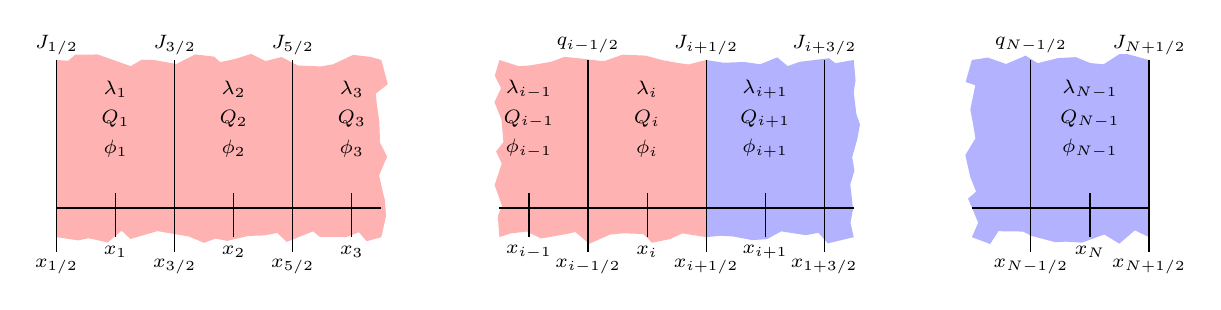
\begin{tikzpicture}[scale=0.75] \scriptsize
% left side boundary section
\fill[red!30, decoration={random steps,segment length=0.2cm}] (0,-0.5) decorate{-- (5.5,-0.5)} decorate{-- (5.5,2.5)} decorate{-- (0,2.5)} -- cycle;
\draw[thick] (0,0) -- (5.5,0);
\draw (0,-0.75) -- (0,2.5);
\draw (1,-0.5)  -- (1,0.25);
\draw (2,-0.75) -- (2,2.5);
\draw (3,-0.5)  -- (3,0.25);
\draw (4,-0.75) -- (4,2.5);
\draw (5,-0.5)  -- (5,0.25);
\node at (0,-1) 	{$x_{1/2}$};
\node at (1,-0.75) 	{$x_1$};
\node at (2,-1) 	{$x_{3/2}$};
\node at (3,-0.75) 	{$x_2$};
\node at (4,-1) 	{$x_{5/2}$};
\node at (5,-0.75) 	{$x_3$};
\node at (0,2.75) {$J_{1/2}$}; \node at (2,2.75) {$J_{3/2}$}; \node at (4,2.75) {$J_{5/2}$};
\node at (1,2)   {$\lambda_1$}; \node at (1,1.5)   {$Q_1$}; 	\node at (1,1)   {$\phi_1$};
\node at (3,2)   {$\lambda_2$}; \node at (3,1.5)   {$Q_2$}; 	\node at (3,1)   {$\phi_2$};
\node at (5,2)   {$\lambda_3$}; \node at (5,1.5)   {$Q_3$}; 	\node at (5,1)   {$\phi_3$};

% interior section
\fill[red!30,  decoration={random steps,segment length=0.2cm}] (7.5,-0.5) decorate{-- (11,-0.5)} -- (11,2.5) decorate{-- (7.5,2.5)} decorate{-- cycle};
\fill[blue!30, decoration={random steps,segment length=0.2cm}] (11,-0.5)  decorate{-- (13.5,-0.5)} decorate{-- (13.5,2.5)} decorate{-- (11,2.5)} -- cycle;
\draw[thick] (7.5,0) -- (13.5,0);
\draw (8, -0.5)   -- (8, 0.25);
\draw (9, -0.75)  -- (9, 2.5);
\draw (10,-0.5)   -- (10,0.25);
\draw (11,-0.75)  -- (11,2.5);
\draw (12,-0.5)   -- (12,0.25);
\draw (13,-0.75)  -- (13,2.5);
%\draw (14,-0.5)   -- (14,0.25);
\node at (8,-0.75) 	{$x_{i-1}$};
\node at (9,-1) 	{$x_{i-1/2}$};
\node at (10,-0.75) {$x_{i}$};
\node at (11,-1) 	{$x_{i+1/2}$};
\node at (12,-0.75) {$x_{i+1}$};
\node at (13,-1) 	{$x_{1+3/2}$};
%\node at (14,-0.75) {$x_{i+2}$};
\node at (9,2.75) {$q_{i-1/2}$}; \node at (11,2.75) {$J_{i+1/2}$}; \node at (13,2.75) {$J_{i+3/2}$};
\node at (8, 2)   {$\lambda_{i-1}$}; 	\node at (8, 1.5) {$Q_{i-1}$}; 	\node at (8, 1)   {$\phi_{i-1}$};
\node at (10,2)   {$\lambda_{i}$}; 		\node at (10,1.5) {$Q_{i}$}; 	\node at (10,1)   {$\phi_{i}$};
\node at (12,2)   {$\lambda_{i+1}$}; 	\node at (12,1.5) {$Q_{i+1}$}; 	\node at (12,1)   {$\phi_{i+1}$};
%\node at (14,2)   {$\Sigma_{i+2}$}; 	\node at (14,1.5) {$q_{i+2}$}; 	\node at (14,1)   {$\phi_{i+2}$};

% interior section
\fill[blue!30,  decoration={random steps,segment length=0.2cm}] (15.5,-0.5) decorate{-- (18.5,-0.5)} -- (18.5,2.5) decorate{-- (15.5,2.5)} decorate{-- cycle};
\draw[thick] (15.5,0) -- (18.5,0);
\draw (18.5, -0.75)   -- (18.5, 2.5);
\draw (17.5, -0.5)  -- (17.5, 0.25);
\draw (16.5, -0.75)  -- (16.5, 2.5);
\node at (16.5,-1) 	{$x_{N-1/2}$};
\node at (17.5,-0.75) {$x_{N}$};
\node at (18.5,-1) 	{$x_{N+1/2}$};
\node at (16.5,2.75) {$q_{N-1/2}$}; \node at (18.5,2.75) {$J_{N+1/2}$};
\node at (17.5, 2)   {$\lambda_{N-1}$}; 	\node at (17.5, 1.5) {$Q_{N-1}$}; 	\node at (17.5, 1)   {$\phi_{N-1}$};

\end{tikzpicture}
\caption{Grid or stencil for the cell-centered finite differencing scheme for the reaction-diffusion equation.}
\label{Fig:ode_reactionDiffusionFiniteDifferenceStencil}
\end{center}
\end{figure}

%\begin{figure}[tb!]
%\begin{center}
%\begin{tikzpicture}
%% left side boundary section
%\fill[red!30, decoration={random steps,segment length=0.2cm}] (0,-0.5) decorate{-- (5.5,-0.5)} decorate{-- (5.5,2.5)} decorate{-- (0,2.5)} -- cycle;
%\draw[thick] (0,0) -- (5.5,0);
%\draw (0,-0.75) -- (0,2.5);
%\draw (1,-0.5)  -- (1,0.25);
%\draw (2,-0.75) -- (2,2.5);
%\draw (3,-0.5)  -- (3,0.25);
%\draw (4,-0.75) -- (4,2.5);
%\draw (5,-0.5)  -- (5,0.25);
%\node at (0,-1) 	{$x_0$};
%\node at (1,-0.75) 	{$x_{1/2}$};
%\node at (2,-1) 	{$x_1$};
%\node at (3,-0.75) 	{$x_{3/2}$};
%\node at (4,-1) 	{$x_2$};
%\node at (5,-0.75) 	{$x_{5/2}$};
%\node at (0,2.75) {$y_0$}; \node at (2,2.75) {$y_1$}; \node at (4,2.75) {$y_2$};
%\node at (1,2)   {$k_{1/2}$}; \node at (1,1.5) {$\lambda_{1/2}$}; \node at (1,1)   {$q_{1/2}$};
%\node at (3,2)   {$k_{3/2}$}; \node at (3,1.5) {$\lambda_{3/2}$}; \node at (3,1)   {$q_{3/2}$};
%\node at (5,2)   {$k_{5/2}$}; \node at (5,1.5) {$\lambda_{5/2}$}; \node at (5,1)   {$q_{5/2}$};
%
%% interior section
%\fill[red!30,  decoration={random steps,segment length=0.2cm}] (7.5,-0.5) decorate{-- (11,-0.5)} -- (11,2.5) decorate{-- (7.5,2.5)} decorate{-- cycle};
%\fill[blue!30, decoration={random steps,segment length=0.2cm}] (11,-0.5)  decorate{-- (14.5,-0.5)} decorate{-- (14.5,2.5)} decorate{-- (11,2.5)} -- cycle;
%\draw[thick] (7.5,0) -- (14.5,0);
%\draw (8, -0.5)   -- (8, 0.25);
%\draw (9, -0.75)  -- (9, 2.5);
%\draw (10,-0.5)   -- (10,0.25);
%\draw (11,-0.75)  -- (11,2.5);
%\draw (12,-0.5)   -- (12,0.25);
%\draw (13,-0.75)  -- (13,2.5);
%\draw (14,-0.5)   -- (14,0.25);
%\node at (8,-0.75) 	{$x_{i-3/2}$};
%\node at (9,-1) 	{$x_{i-1}$};
%\node at (10,-0.75) {$x_{i-1/2}$};
%\node at (11,-1) 	{$x_{i}$};
%\node at (12,-0.75) {$x_{i+1/2}$};
%\node at (13,-1) 	{$x_{1+1}$};
%\node at (14,-0.75) {$x_{i+3/2}$};
%\node at (9,2.75) {$y_{i-1}$}; \node at (11,2.75) {$y_i$}; \node at (13,2.75) {$y_{i+1}$};
%\node at (8, 2)   {$k_{i-3/2}$}; 	\node at (8, 1.5) {$\lambda_{i-3/2}$}; 	\node at (8, 1)   {$q_{i-3/2}$};
%\node at (10,2)   {$k_{i-1/2}$}; 	\node at (10,1.5) {$\lambda_{i-1/2}$}; 	\node at (10,1)   {$q_{i-1/2}$};
%\node at (12,2)   {$k_{i+1/2}$}; 	\node at (12,1.5) {$\lambda_{i+1/2}$}; 	\node at (12,1)   {$q_{i+1/2}$};
%\node at (14,2)   {$k_{i+3/2}$}; 	\node at (14,1.5) {$\lambda_{i+3/2}$}; 	\node at (14,1)   {$q_{i+3/2}$};
%\end{tikzpicture}
%\caption{Grid or stencil for the finite differencing scheme for the reaction-diffusion equation.}
%\label{Fig:ode_reactionDiffusionFiniteDifferenceStencil}
%\end{center}
%\end{figure}

A common boundary value problem that arises in engineering applications is the reaction-diffusion equation:
\begin{align}
  -\frac{d}{dx} \left( D(x) \frac{d\phi}{dx} \right) + \lambda(x) \phi(x) = Q(x) ,
\end{align}
where $\phi(x)$ is some spatially dependent physical quantity and $Q(x)$ is an internal source. We define the flow rate across some interface as
\begin{align}
  J(x) = -D(x) \frac{d\phi}{dx} . \label{Eq:ode_finiteDifference_reactionDiffusion_flowRate}
\end{align}
This equation arises in applications including the analysis of viscous fluids in laminar flow, structural mechanics, heat conduction, and neutron diffusion. Here $D(x)$ is a diffusion coefficient and $\lambda(x)$ is a reaction coefficient. The former describes the local rate that the physical quantity of the field spreads out, and the latter describes the local rate that the field is created or destroyed in proportion to itself. The right-hand side has an inhomogeneous term for the field being created (e.g., heat generation from nuclear reactions or the creation of neutrons from fission).

To apply the finite difference approximation we need to define a spatial grid or stencil. There are many strategies employed and here we present a scheme that is intended to conserve physical quantities within each spatial cell, i.e. the rate of production of some quantity within a cell plus the rate that the quantity flows in equals the rate that it is destroyed within the cell plus the rate it flows out. This sounds rather obvious and we had not had to worry about it because the differential equations (either neutron transport or diffusion) naturally support particle balance by virtue of how they were derived. The problem is that the process of mapping these differential equations onto a spatial discretization, which converts a calculus problem into algebra one, may or may not preserve the balance of particles depending on how this is done. 

To this end, we introduce the \emph{cell-centered} spatial discretization, which is depicted in Fig.~\ref{Fig:ode_reactionDiffusionFiniteDifferenceStencil}. The cell-centered spatial discretization breaks the problem into $N$ spatial regions indexed from $i = 1, 2, \ldots, N$ (note that many programming language index from zero, so implementations need to subtract one from each index) each having a width $\Delta_i = x_{i+1} - x_i$. The point $x_i$ is the center of the $i$th spatial zone. This implies that $x_{1/2} = 0$ is the left edge of the slab and $x_{N+1/2}$ is the right edge. Material properties and sources are taken to be constant within each spatial zone. Ideally, we choose the spatial discretization to line up with the geometric regions of the problem. If we cannot do this, or do not wish to for some reason, then we need to find some average value of the material properties.

\subsubsection{Discretion of the Continuity Equation}

To derive the discretization scheme, we first insert the definition of the flow rate into the reaction-diffusion equation to obtain a \emph{continuity equation}:
\begin{align}
  \frac{dJ}{dx} + \lambda(x) \phi(x) = Q(x) .
\end{align}
A continuity equation states that the local net outflow rate $dJ/dx$ (proportional to the spatial gradient of a physical quantity) plus the internal loss rate equals the gain rate. 

We then integrate over a spatial region:
\begin{align}
  &\int_{x_{i-1/2}}^{x_{i+1/2}} \frac{dJ}{dx} + \lambda(x) \phi(x) dx = \int_{x_{i-1/2}}^{x_{i+1/2}} Q(x) dx, \nonumber \\
  &J_{i+1/2} - J_{i-1/2} + \int_{x_{i-1/2}}^{x_{i+1/2}} \lambda(x) \phi(x) dx = \int_{x_{i-1/2}}^{x_{i+1/2}} Q(x) dx .
\end{align}
Since the reaction coefficient is assumed to be spatially constant over the region and equal to $\lambda_i$, we can pull it out of the integral. Next, we define the cell-average quantity and source to be at the center of the cell,
\begin{subequations}
\begin{align}
  \phi_i 	&= \frac{1}{\Delta_i} \int_{x_{i-1/2}}^{x_{i+1/2}} \phi(x) dx , \\
  Q_i 		&= \frac{1}{\Delta_i} \int_{x_{i-1/2}}^{x_{i+1/2}} Q(x) dx .
\end{align}
\end{subequations}
Inserting these cell-averaged quantities and sources we get
\begin{align}
  J_{i+1/2} - J_{i-1/2} + \lambda_i \Delta_i \phi_i = Q_i \Delta_i .
\end{align}
The next task is to figure out the flow rates at the cell-edges. 

\subsubsection{Interface Conditions for Internal Regions}

We handle the flow rates differently if the cell is an internal region versus a boundary region. First we explore the internal regions, which require us to use the interface condition that the net current must be continuous. Beginning on the left-hand side of a cell centered at $x_i$, we apply both the forward and backward differencing schemes to Eq.~\eqref{Eq:ode_finiteDifference_reactionDiffusion_flowRate} to relate the flow rates $J$ on each edge with the physical quantities $u$,
\begin{subequations}
\begin{align}
  J_{i-1/2} &= -D_{i}   \frac{ \phi_{i}     - \phi_{i-i/2} }{ \Delta_{i}/2 }, \label{Eq:ode_finiteDifference_reactionDiffusion_FicksLawLeftInterface1} \\
  J_{i-1/2} &= -D_{i-1} \frac{ \phi_{i-1/2} - \phi_{i-1}   }{ \Delta_{i-1}/2 },
\end{align}
\end{subequations}
for the element centered about $x_i$ and $x_{i-1}$ respectively. Note the factor of one-half on the width of the cell is because we take the finite difference to approximate the derivative from the center to the edge, which is half the width.

Both of these equations involve the quantity of interest at the cell edge $\phi(x_{i-1/2}) = \phi_{i-1/2}$, which is not part of the discretized continuity equation. However, since we have two equations in terms of the cell-edge quantity and the flow rate at that edge, we can eliminate this extra variable by equating the two equations and solving for $\phi_{i-1/2}$. After a bit of algebra, we get
\begin{align}
  \phi_{i-1/2} = \left[ \frac{ D_{i-1} / \Delta_{i-1} }{ D_{i-1}/\Delta_{i-1} + D_{i}/\Delta_{i} } \right] \phi_{i-1} + \left[ \frac{ D_i / \Delta_i }{ D_{i-1}/\Delta_{i-1} + D_{i}/\Delta_{i} } \right] \phi_i . 
\end{align}
If we inspect the terms of brackets, we can see see that if we were to add them together, we would get one. Therefore, we define the term on the left as $\omega_{i-1}$ and have $\omega_i = 1 - \omega_{i-1}$. This allows us to write this more compactly as
\begin{align}
  \phi_{i-1/2} = \omega_{i-1} \phi_{i-1} + ( 1 - \omega_{i-1} ) \phi_i .
\end{align}
Inserting this into Eq.~\eqref{Eq:ode_finiteDifference_reactionDiffusion_FicksLawLeftInterface1}, we can then solve for the flow rate at the left interface:
\begin{align}
  J_{i-1/2} &= -\frac{2 D_{i}}{\Delta_i} \left[ \phi_i - \omega_{i-1} \phi_{i-1} - ( 1 - \omega_{i-1} ) \phi_i \right] \nonumber \\
  			&= -\frac{2 D_{i} \omega_{i-1} }{\Delta_i} ( \phi_i - \phi_{i-1} ) \nonumber \\
			&= -2 \frac{ ( D_{i-1} / \Delta_{i-1} ) ( D_i / \Delta_i ) }{ D_{i-1} / \Delta_{i-1} + D_i / \Delta_i } ( \phi_i - \phi_{i-1} ) \nonumber \\
			&= -\widetilde{D}_{i-1/2} ( \phi_i - \phi_{i-1} ) .
\end{align}

Here we defined as shorthand the edge-averaged diffusion coefficient
\begin{align}
  \widetilde{D}_{i-1/2} = 2 \frac{ ( D_{i-1} / \Delta_{i-1} ) ( D_i / \Delta_i ) }{ D_{i-1} / \Delta_{i-1} + D_i / \Delta_i } . \label{Eq:ode_finiteDifference_reactionDiffusion_EdgeAverageDiffusionCoefficient}
\end{align}
At first glance, this may not look like much of an average, but if we set the cell widths to be equal, we can show that this is the harmonic mean of the diffusion coefficients. (Note that this is different than what is sometimes used for the diffusion coefficients in standard finite difference methods where the they are taken in an ad hoc manner to be the arithmetic mean.)

We can repeat the process for the flow rate on the right edge $J_{1+1/2}$ by consider the cell at $x_i$ and the one to the right centered about $x_{i+1}$. Applying the finite difference on both sides of the edge gives
\begin{subequations}
\begin{align}
  J_{i+1/2} &= -D_{i}   \frac{ \phi_{i+1/2} - \phi_{i} 		}{ \Delta_{i}/2 	}, \label{Eq:ode_finiteDifference_reactionDiffusion_FicksLawRightInterface1} \\
  J_{i+1/2} &= -D_{i+1} \frac{ \phi_{i} 	- \phi_{i-1/2}  }{ \Delta_{i+1}/2 	}.
\end{align}
\end{subequations}
Setting these equal and solving for the cell-edge scalar flux gives
\begin{align}
  J_{i+1/2} &=  \left[ \frac{ D_i / \Delta_i }{ D_{i+1}/\Delta_{i+1} + D_{i}/\Delta_{i} } \right] \phi_i + \left[ \frac{ D_{i+1} / \Delta_{i+1} }{ D_{i+1}/\Delta_{i+1} + D_{i}/\Delta_{i} } \right] \phi_{i+1} \nonumber \\
  &= \omega_i \phi_i + ( 1 - \omega_i ) \phi_{i+1},
\end{align}
again noting the terms in brackets sum to one. Inserting this into Eq.~\eqref{Eq:ode_finiteDifference_reactionDiffusion_FicksLawRightInterface1} to eliminate the cell-edge quantity, we get
\begin{align}
  J_{i+1/2} &= -\frac{2 D_{i}}{\Delta_i} \left[ \omega_i \phi_i + ( 1 - \omega_i ) \phi_{i+1} - \phi_{i}  \right] \nonumber \\
  			&= -\frac{2 D_{i} ( 1- \omega_{i-1} ) }{\Delta_i} ( \phi_{i+1} - \phi_i ) \nonumber \\
			&= -2 \frac{ ( D_{i} / \Delta_{i} ) ( D_{i+1} / \Delta_{i+1} ) }{ D_{i} / \Delta_{i} + D_{i+1} / \Delta_{i+1} } ( \phi_{i+1} - \phi_{i} ) \nonumber \\
			&= -\widetilde{D}_{i+1/2} ( \phi_{i+1} - \phi_{i} ) .
\end{align}
Here again, the edge-averaged diffusion coefficient
\begin{align}
  \widetilde{D}_{i+1/2} = 2 \frac{ ( D_{i} / \Delta_{i} ) ( D_{i+1} / \Delta_{i+1} ) }{ D_{i} / \Delta_{i} + D_{i+1} / \Delta_{i+1} } .
\end{align}
Note that this coefficient is identical to the one in Eq.~\eqref{Eq:ode_finiteDifference_reactionDiffusion_EdgeAverageDiffusionCoefficient} by letting $i \rightarrow i+1$, which is comforting.

Plugging these edge net currents back into the discretized continuity equation, we have
\begin{align}
  -\widetilde{D}_{i+1/2} ( \phi_{i+1} - \phi_{i} ) + \widetilde{D}_{i-1/2} ( \phi_i - \phi_{i-1} )  + \lambda_i \Delta_i \phi_i = Q_i \Delta_i .
\end{align}
Grouping terms we get
\begin{align}
 -\widetilde{D}_{i-1/2} u_{i-1} + \left( \widetilde{D}_{i-1/2} + \widetilde{D}_{i+1/2}  + \lambda_i \Delta_i \right) \phi_i - \widetilde{D}_{i+1/2} \phi_{i+1}  = Q_i \Delta_i .
\end{align}

If we inspect this expression for the cell centered at $x_i$, we notice that its average quantity $u_i$ is coupled only to the average quantities to its immediate neighbors. If we write out the equations for each of the interior mesh cells, $i=1, \ldots, N-2$, (we address the boundary cells next) we notice that this forms a tridiagonal system of equations. We can therefore write the coefficients as the subdiagonal (lower) element $\ell_i$, diagonal element $d_i$, the superdiagonal (upper) element $u_i$, and the right-hand side vector element $r_i$ as
\begin{subequations}
\begin{align}
  \ell_i	&= -\widetilde{D}_{i-1/2}, \\
  d_i		&=  \widetilde{D}_{i-1/2} + \widetilde{D}_{i+1/2}  + \lambda_i \Delta_i, \\
  u_i		&= -\widetilde{D}_{i+1/2}, \\
  r_i		&=  Q_i \Delta_i.
\end{align} 
\end{subequations}
These interior cell equations may then be written generically as
\begin{align}
  \ell_i \phi_{i-1} + d_i \phi_i + u_i \phi_{i+1} = r_i .
\end{align}
It turns out that we get pretty much the exact same results on the boundaries as well. One difference is that on the left and right sides at $i = 0$ and $i = N-1$ we have
\begin{subequations}
\begin{align}
  \ell_0  = 0, \\*
  u_{N-1} = 0,
\end{align}
\end{subequations}
which would be outside the bounds of the matrix. We also can get an additional term on the right-hand side vector should there be an inward partial current. Of course, we still need to actually compute the edge diffusion coefficients, which is the next topic.


\subsubsection{Boundary Conditions}

We can write the boundary condition generically as
\begin{align}
  \alpha \phi + \beta J = \gamma ,
\end{align}
where $\alpha$, $\beta$, and $\gamma$ are given coefficients. On the left boundary we give them an $\ell$ subscript and an $r$ subscript on the right boundary.

We first derive the boundary condition on the left side. The continuity equation is
\begin{align}
  J_{3/2} - J_{1/2} + \lambda_1 \Delta_1 \phi_1 = Q_1 \Delta_1 .
\end{align}
From the analysis for interior elements, we have
\begin{align}
  J_{3/2} = -\widetilde{D}_{3/2} ( \phi_2 - \phi_1 ) .
\end{align}
The task then is to figure out the flow rate at the boundary $J_{1/2}$ in terms of the quantities of interest and the boundary condition.

Applying the finite difference rule to connect the left edge to the interior, we have
\begin{align}
  J_{1/2} = -D_1 \frac{ \phi_1 - \phi_{1/2} }{ \Delta_1 / 2 } .
\end{align}
Next, we perform some algebra to obtain
\begin{align}
  ( 2 D_1 / \Delta_1 ) \phi_{1/2} = J_{1/2} + ( 2 D_1 / \Delta_1 ) \phi_1 .
\end{align}
Next, we multiply the left boundary condition by $2 D_1 / \Delta_1$,
\begin{align}
  ( 2 D_1 / \Delta_1 ) \alpha_\ell \phi_{1/2} + ( 2 D_1 / \Delta_1 ) \beta_\ell J_{1/2} = ( 2 D_1 / \Delta_1 ) \gamma_\ell,
\end{align}
substitute in for the quantity at the boundary and solve for the flow rate as
\begin{align}
  J_{1/2} = - \frac{ 2 D_1 / \Delta_1 }{ \alpha_\ell + \beta_\ell ( 2 D_1 / \Delta_1 ) } \alpha_\ell \phi_1 + \frac{ 2 D_1 / \Delta_1 }{ \alpha_\ell + \beta_\ell ( 2 D_1 / \Delta_1 ) } \gamma_\ell .
\end{align}
We can define the edge-averaged diffusion coefficient on the left boundary as
\begin{align}
  \widetilde{D}_{1/2} = \frac{ 2 D_1 / \Delta_1 }{ \alpha_\ell + \beta_\ell ( 2 D_1 / \Delta_1 ) } .
\end{align}
We then have the flow rate on the left boundary as
\begin{align}
  J_{1/2} = -\widetilde{D}_{1/2} \alpha_\ell \phi_1 + \widetilde{D}_{1/2} \gamma_\ell .
\end{align}
This result appears similar to what we found for the interior element except there is an additional factor of $\alpha_\ell$ on the edge-average diffusion coefficient and there is another term for the inflow of the quantity given by $\gamma$.

Inserting the flow rates into the continuity equation gives
\begin{align}
  -\widetilde{D}_{3/2} ( \phi_2 - \phi_1 ) + \widetilde{D}_{1/2} \alpha_\ell \phi_1 - \widetilde{D}_{1/2} \gamma_\ell + \lambda_1 \Delta_1 \phi_1 = Q_1 \Delta_1 .
\end{align}
After some rearrangement, we obtain
\begin{align}
  \left( \widetilde{D}_{1/2} \alpha_\ell + \widetilde{D}_{3/2} + \lambda_1 \Delta_1 \right) \phi_1 - \widetilde{D}_{3/2} \phi_2 = Q_1 \Delta_1 + \widetilde{D}_{1/2} \gamma_\ell .
\end{align}

We can repeat the analysis on the right boundary. The continuity equation is
\begin{align}
  J_{N+1/2} - J_{N-1/2} + \lambda_{N} \Delta_{N} \phi_{N} = Q_{N} \Delta_{N} .
\end{align}
Since $J_{N-1/2}$ is for an interior element,
\begin{align}
  J_{N-1/2} = -\widetilde{D}_{N-1/2} ( \phi_{N} - \phi_{N-1} ) .
\end{align}
Apply the finite difference rule on the right edge,
\begin{align}
  J_{N+1/2} = -D_{N} \frac{ \phi_{N+1/2} - \phi_{N} }{ \Delta_{N} / 2 } ,
\end{align}
and obtain
\begin{align}
  ( 2 D_{N} / \Delta_{N} ) \phi_{N+1/2} = -J_{N+1/2} + ( 2 D_{N} / \Delta_{N} ) \phi_{N} .
\end{align}
Multiplying the boundary condition as before by $2 D_{N-1} / \Delta_{N-1}$,
\begin{align}
  ( 2 D_{N} / \Delta_{N} ) \alpha_r \phi_{N+1/2} + ( 2 D_{N} / \Delta_{N} ) \beta_r J_{N+1/2} = ( 2 D_{N} / \Delta_{N} ) \gamma_r,
\end{align}
% \alpha_r ( -J_{N-1/2} + ( 2 D_{N-1} / \Delta_{N-1} ) \phi_{N-1} )  + ( 2 D_{N-1} / \Delta_{N-1} ) \beta_r J_{N-1/2} = ( 2 D_{N-1} / \Delta_{N-1} ) \gamma_r
% -\alpha_r J_{N-1/2} + ( 2 D_{N-1} / \Delta_{N-1} ) \alpha_r \phi_{N-1}  + ( 2 D_{N-1} / \Delta_{N-1} ) \beta_r J_{N-1/2} = ( 2 D_{N-1} / \Delta_{N-1} ) \gamma_r
% -\alpha_r J_{N-1/2} + ( 2 D_{N-1} / \Delta_{N-1} ) \beta_r J_{N-1/2} = -( 2 D_{N-1} / \Delta_{N-1} ) \alpha_r \phi_{N-1} + ( 2 D_{N-1} / \Delta_{N-1} ) \gamma_r
% ( -\alpha_r + \beta_r ( 2 D_{N-1} / \Delta_{N-1} ) ) J_{N-1/2} = -( 2 D_{N-1} / \Delta_{N-1} ) \alpha_r \phi_{N-1} + ( 2 D_{N-1} / \Delta_{N-1} ) \gamma_r
% (  \alpha_r - \beta_r ( 2 D_{N-1} / \Delta_{N-1} ) ) J_{N-1/2} =  ( 2 D_{N-1} / \Delta_{N-1} ) \alpha_r \phi_{N-1} - ( 2 D_{N-1} / \Delta_{N-1} ) \gamma_r
and making the substitution gives
\begin{align}
  J_{N+1/2} = \widetilde{D}_{N+1/2} \alpha_r \phi_{N} - \widetilde{D}_{N+1/2} \gamma_r,
\end{align}
where the edge-averaged diffusion coefficient is
\begin{align}
  \widetilde{D}_{N+1/2} = \frac{ 2 D_{N} / \Delta_{N} }{ \alpha_r - \beta_r ( 2 D_{N} / \Delta_{N} ) } .
\end{align}
Substituting into the continuity equation and rearranging gives a very similar result to that of the left boundary
\begin{align}
  -\widetilde{D}_{N-1/2} \phi_{N-1} + \left( \widetilde{D}_{N-1/2} + \widetilde{D}_{N+1/2} \alpha_r + \lambda_{N} \Delta_{N} \right) \phi_{N} = Q_{N} \Delta_{N} + \widetilde{D}_{N+1/2} \gamma_r .
\end{align}

We can then use these boundary results to define the coefficients of the tridiagonal matrix and right-hand side vector elements. On the left boundary (top row) we have
\begin{subequations}
\begin{align}
  d_1 &= \widetilde{D}_{1/2} \alpha_\ell + \widetilde{D}_{3/2} + \lambda_1 \Delta_1, \\
  u_1 &= - \widetilde{D}_{3/2}, \\
  r_1 &= Q_1 \Delta_1 + \widetilde{D}_{1/2} \gamma_\ell .
\end{align}
And on the right boundary (bottom row) we have
\begin{align}
  \ell_{N} &= -\widetilde{D}_{N-1/2} , \\
  d_{N}	   &= \widetilde{D}_{N-1/2} + \widetilde{D}_{N+1/2} \alpha_r + \lambda_{N} \Delta_{N} , \\
  r_{N}    &= Q_{N} \Delta_{N} + \widetilde{D}_{N+1/2} \gamma_r 
\end{align}
\end{subequations}

Comparing these with the interior elements, we note two key differences. First, for the diagonal element the edge-average diffusion coefficient has an additional factor of $\alpha$. Second, there is an extra term on the right-hand side vector $\gamma$ that typically denotes flow of the quantity of interest into the problem domain from the exterior.

We also consider a couple special cases. The first is the Dirichlet boundary condition where $\alpha = 1, \beta = 0$, and $\gamma = \phi_b$ where $\phi_b$ is some known boundary value. The edge-average diffusion coefficient at the left boundary becomes
\begin{align}
  \widetilde{D}_{1/2} = \frac{2 D_1}{\Delta_1},
\end{align}
and similarly on the right.

Another special case is the Neumann boundary condition where there is no net inflow of the quantity. This is $\alpha = 0$, $\beta = 1$, $\gamma = 0$. Since $\alpha = \gamma = 0$, the edge-average diffusion coefficient vanishes from the expressions.



%
%\clearpage
%
%
%
%For reaction-diffusion problems we define the field $y(x)$ to be defined on the grid points $y(x_i) = y_i$. The diffusion coefficient $k(x)$, reaction coefficient $\lambda(x)$, and the source term $q(x)$, are however defined on the interior of the element between the grid points, which we often write using half indices, $k(x_{i+1/2}) = k_{i+1/2}$. Specifying the problem in this manner allows us to enforce conservation laws (e.g., energy, particles, etc.) and gives us a higher quality solution. 
%
%An illustration of the discretization scheme is provided in Fig.~\ref{Fig:ode_reactionDiffusionFiniteDifferenceStencil}. At the left is the left-hand boundary at a point with a position $x_0$. The leftmost element or zone exists between $x_0 \le x < x_1$, where the zone properties, diffusion coefficient $k_{1/2}$, absorption coefficient $\lambda_{1/2}$, and internal source $q_{1/2}$, are defined at the midpoint with the half index. The field $y_0$ and $y_1$ is defined at the boundaries. On the right is an interior element. The indexing is much the same as on the left, except that in this illustration there is an interface between two materials at location $x_i$ (note that this is just an example of a location of an interface, which could be at any of the grid points), denoted by the different colors on the left and right sides of $x_i$. While not shown in the illustration, the portion for the right boundary would be a reflection of the portion on the left, except that the indexing would end at $x_N$.
%
%We then need to map the diffusion operator on the first term onto our spatial grid. This operator has two applications of the first derivative (if the diffusion coefficient does not depend on space, then we can write it as a second derivative and apply the approximation from the previous section), for which we can apply central difference twice. We apply the inner derivative to map the field onto the half indices using central difference:
%\begin{align}
%  \frac{dy}{dx} = \frac{ y_{i+1/2} - y_{i-1/2} }{ \Delta x } + \mathcal{O}(\Delta x^2) .
%\end{align}
%To be consistent, we need to, however, (temporarily) define the diffusion coefficient at the central grid point. Applying the central difference again moves each term another half index. Taking the central difference on the first term gives
%\begin{subequations}
%\begin{align}
%  \frac{d}{dx} \left[ \frac{ k_i y_{i+1/2} }{ \Delta x } \right] = \frac{ k_{i+1/2} y_{i+1} - k_{i-1/2} y_i }{ ( \Delta x )^2 } + \mathcal{O}(\Delta x^2) .
%\end{align}
%The central difference of the second term is
%\begin{align}
%  \frac{d}{dx} \left[ \frac{ k_i y_{i-1/2} }{ \Delta x } \right] = \frac{ k_{i+1/2} y_{i} - k_{i-1/2} y_{i-1} }{ ( \Delta x )^2 } + \mathcal{O}(\Delta x^2) .
%\end{align}
%\end{subequations}
%Combining these terms gives
%\begin{align}
%  \frac{d}{dx} \left( k(x) \frac{dy}{dx} \right) = \frac{ k_{i+1/2} y_{i+1} - ( k_{i-1/2} +  k_{i+1/2} ) y_{i} + k_{i-1/2} y_{i-1} }{ ( \Delta x )^2 } +  \mathcal{O}(\Delta x^2).
%\end{align}
%Note that if the diffusion coefficient is the same for both zones surrounding $x_i$, then all the terms in parentheses work out to be $k/(\Delta x)^2$, which can be recast as our standard approximation for the second derivative. The only place where there is a difference is on the interfaces.
%
%Before we can complete the finite differencing scheme, we need to decide how to treat the reaction and source terms. Since the reaction coefficient and source are defined between the grid points, we often assume that the value at the grid point is the arithmetic mean of the two surrounding grid points:
%\begin{subequations}
%\begin{align}
%  \lambda_i &= \frac{ \lambda_{i-1/2} + \lambda_{i+1/2} }{2}, \\
%  q_i 		&= \frac{ \lambda_{i-1/2} + \lambda_{i+1/2} }{2}.
%\end{align}
%\end{subequations}
%%Note that if the diffusion coefficient varies continuously in space, sometimes we define the diffusion coefficients as the arithmetic mean of the diffusion coefficients at grid points
%%\begin{align}
%%  k_{i-1/2} = \frac{ k_{i-1} + k_{i} }{2}, \quad k_{i+1/2} = \frac{ k_{i} + k_{i+1} }{2} , \nonumber
%%\end{align}
%%but we will assume that the diffusion coefficients are spatially constant within a region and not use this. 
%
%Applying this approximation and regrouping some terms, we can write the finite-difference approximation of the reaction-diffusion equation:
%\begin{align}
%   -  \left[ \frac{ k_{i-1/2} }{ ( \Delta x )^2 } \right] y_{i-1} 
%   +  \left[ \frac{ k_{i-1/2} +  k_{i+1/2} }{ ( \Delta x )^2 } + \lambda_i \right] y_{i} 
%   -  \left[ \frac{ k_{i+1/2} }{ ( \Delta x )^2 } \right] y_{i+1} = q_i .
%\end{align}
%
%This equation contains only points at $x_i$ and at the two adjacent grid points. If we specify this equation at all points $i = 0, \ldots, N$ (ignoring the boundaries for now) then we get a system that is tridiagonal and can be solved directly and very efficiently as $O(N)$, linear scaling with the size of the grid. Adopting the notation of diagonal, subdiagonal, and superdiagonal terms from Sec.~\ref{Sec:linearAlgebra_SystemsOfLinearEquations_TridiagonalSystems}, we have
%\begin{subequations}
%\begin{align}
%  \ell_i	&= -\frac{ k_{i-1/2} }{ \Delta x  }, \quad i = 2, \ldots, N-1, \\*
%  d_i 		&= \frac{ k_{i-1/2} +  k_{i+1/2} }{ \Delta x } + \lambda_i \Delta x, \quad i = 1, \ldots, N-1, \\*
%  u_i		&= -\frac{ k_{i+1/2} }{ \Delta x  }, \quad i = 1, \ldots, N-1, \\*
%  r_i		&= q_i \Delta x, \quad i = 1, \ldots, N-1.
%\end{align}
%\end{subequations}
%Here we multiplied the equation by $\Delta x$. This helps prevent terms from becoming very large with $\Delta x$ gets small, which can lead to numerical instabilities.
%
%%%%%%%%%%%%%%%%%%%%%%%%%%%%%%%%%%%%%%%%%%%%%%%%%%%%%%%%%%%%%%%%%%%%%%%%%%%%%%%%%%%%%%%%%%%%%%%%
%\subsection{Approximation of the Boundary Conditions} \label{Sec:ode_finiteDifference_boundaryConditions}
%
%The previous section established the finite-differencing scheme for the reaction-diffusion problem. This is valid for the interior grid points, but special handling is required for the boundary conditions. We can represent any of the three standard types of boundary conditions as
%\begin{align}
%  \alpha y + \beta \frac{dy}{dx} = \gamma,
%\end{align}
%where $y$ and $dy/dx$ are evaluated at the boundary and $\alpha$, $\beta$, and $\gamma$ are coefficients that depend upon the context of the problem.
%
%The first case is the Dirichlet boundary condition, which takes $\beta = 0$. This reduces to specifying the value of $u$ on the boundary, given by $\alpha / \gamma$. In this case, we usually just write $\gamma / \alpha$ as $y_0$ on the left and $y_N$ on the right. On the left-hand side, the Dirichlet condition elements of the tridiagonal system become:
%\begin{subequations}
%\begin{align}
%  d_0 		&= 1, \\*
%  u_0		&= 0, \\*
%  r_0		&= q_0 \Delta x + y_0.
%\end{align}
%On the right side, these are:
%\begin{align}
%  \ell_N 	&= 0, \\*
%  d_N		&= 1, \\*
%  r_N		&= q_N \Delta x + y_N.
%\end{align}
%\end{subequations}
%
%The Neumann and Robin (mixed) boundary conditions are best derived together. In both cases $\beta \ne 0$. In the Neumann case, $\alpha = 0$. As we will soon see, the formula in the Neumann boundary condition is a special case of the Robin boundary condition.
%
%The issue with either case is that we must define the derivative at the boundary; however, if we are using a differencing scheme, we do not have a point to define the field to compute the slope at. The usual approach is to extend or extrapolate the spatial grid by one grid element with a fictitious or \emph{ghost} grid point. This ghost point only exists temporarily for the purpose of the derivation and does not appear in the final form of the coefficients.
%
%To begin, we use the finite difference representation of the equation at the boundary as if it were an interior point. For the left-hand side, this is
%\begin{align}
%   -   \left[ \frac{ k_{-1/2}}{ ( \Delta x )^2 } \right] y_{-1} 
%   +   \left[ \frac{ k_{-1/2} + k_{1/2} }{ ( \Delta x )^2 } + \lambda_0 \right] y_{0} 
%   -   \left[ \frac{ k_{1/2} }{ ( \Delta x )^2 } \right] y_{1} = q_0 .
%\end{align}
%We then let the diffusion coefficients outside the region equal to the point on the interior boundary element: here $k_{-1/2} = k_{1/2}$. The argument for doing this is that it should preserve the overall slope of the function. This yields,
%\begin{align}
%   -   \left[ \frac{ k_{1/2}}{ ( \Delta x )^2 } \right] y_{-1} 
%   +   \left[ \frac{ 2 k_{1/2} }{ ( \Delta x )^2 } + \lambda_0 \right] y_{0} 
%   -   \left[ \frac{ k_{1/2} }{ ( \Delta x )^2 } \right] y_{1} = q_0 .
%\end{align}
%We now have unknown values of the field at the extrapolated ghost point element $y_{-1}$. We somehow need to eliminate these to close the system. How this is done is we apply the central differencing scheme to the general mixed boundary condition and solve for this value in a manner that we assert a consistency between the differential equation and the boundary condition. This is
%\begin{align}
%  &\alpha_0 y_0 + \beta_0 \frac{y_1 - y_{-1}}{2 \Delta x} = \gamma_0.
%\end{align}
%Here we give the coefficients a superscript since they are often different on the left and right sides. Then, we can solve for the value at the ghost point:
%\begin{align}
%  y_{-1} 	&= \left( \frac{2 \alpha_0 \Delta x }{\beta_0}  \right) y_0 + y_1 - \frac{2 \Delta x}{\beta_0}  \gamma_0 .
%\end{align}
%Now let us apply the $y_{-1}$ term to the finite difference equation on the left:
%\begin{align}
%   &-  \left[ \frac{   k_{1/2} }{ ( \Delta x )^2 } \right] \left[  \frac{2 \alpha_0 \Delta x }{\beta_0} y_0 + y_1 - \frac{2 \Delta x}{\beta_0} \gamma_0 \right] \nonumber \\*
%   &+  \left[ \frac{ 2 k_{1/2} }{ ( \Delta x )^2 } + \lambda_0 \right] y_{0} 
%   -   \left[ \frac{   k_{1/2} }{ ( \Delta x )^2 } \right] y_{1} = q_0 ,
%\end{align}
%Expanding out the first term,
%\begin{align}
%	&-\frac{2 k_{1/2} \alpha_0}{\beta_0 \Delta x } y_0 - \frac{k_{1/2}}{ ( \Delta x )^2 } y_1 + \frac{2 k_{1/2} }{\beta_0 \Delta x } \gamma_0 \nonumber \\*
%   	&+  \left[ \frac{ 2 k_{1/2} }{ ( \Delta x )^2 } + \lambda_0 \right] y_{0} 
%   	 -  \left[ \frac{ k_{1/2} }{ ( \Delta x )^2 } \right] y_{1} = q_0 ,
%\end{align}
%Combining terms and multiplying through by $\Delta x$ we have
%\begin{align}
%	& \left[ \frac{2 k_{1/2}}{\Delta x} - \frac{2 k_{1/2} \alpha_0}{\beta_0} + \lambda_0 \Delta x \right] y_0
%	- \left[ \frac{2 k_{1/2}}{\Delta x} \right] y_1
%	= q_0 \Delta x - \frac{ 2 k_{1/2} \gamma_0 }{\beta_0} .
%\end{align}
%
%We can repeat this process on the right side. We have
%\begin{align}
%   -   \left[ \frac{ k_{N-1/2} }{ ( \Delta x )^2 } \right] y_{N-1} 
%   +   \left[ \frac{ k_{N-1/2} + k_{N+1/2} }{ ( \Delta x )^2 } + \lambda_N \right] y_{N} 
%   -   \left[ \frac{ k_{N+1/2} }{ ( \Delta x )^2 } \right] y_{N+1} = q_N .
%\end{align}
%Let the diffusion coefficients outside the region equal to the point on the interior boundary element, $k_{N+1/2} = k_{N-1/2}$, giving
%\begin{align}
%   -   \left[ \frac{ k_{N-1/2} }{ ( \Delta x )^2 } \right] y_{N-1} 
%   +   \left[ \frac{ 2 k_{N-1/2} }{ ( \Delta x )^2 } + \lambda_N \right] y_{N} 
%   -   \left[ \frac{ k_{N-1/2} }{ ( \Delta x )^2 } \right] y_{N+1} = q_N .
%\end{align}
%Applying the boundary condition on the right,
%\begin{align}
%  &\alpha_N y_N + \beta_N \frac{y_{N+1} - y_{N}}{2 \Delta x} = \gamma_N.
%\end{align}
%Then, we solving for the value at the ghost point
%\begin{align}
%  y_{N+1}	&= y_{N-1} - \left( \frac{2 \alpha_N \Delta x }{\beta_N}  \right) y_N + \frac{2 \Delta x}{\beta_N} \gamma_N ,
%\end{align}
%From here, insert the $y_{N+1}$ term into the differenced differential equation as before and group terms to obtain:
%\begin{align}
%	- \left[ \frac{2 k_{N-1/2}}{\Delta x} \right] y_{N-1}
%	+ \left[ \frac{2 k_{N-1/2}}{\Delta x} + \frac{2 k_{N-1/2} \alpha_N}{\beta_N} + \lambda_N \Delta x  \right] y_N
%	= q_N \Delta x + \frac{ 2 k_{N-1/2} \gamma_N }{\beta_N} .
%\end{align}
%
%Writing this in terms of the notation for the tridiagonal solve, we have on the left
%\begin{subequations}
%\begin{align}
%  d_0 		&= \frac{2k_{1/2}}{\Delta x} - \frac{2 k_{1/2} \alpha_0}{\beta_0} + \lambda_0 \Delta x, \\*
%  u_0		&= -\frac{2k_{1/2}}{\Delta x}, \\*
%  r_0		&= q_0 \Delta x - \frac{ 2 k_{1/2} \gamma_0 }{\beta_0} ;
%\end{align}
%and on the right,
%\begin{align}
%  \ell_N 	&= -\frac{2 k_{N-1/2}}{\Delta x}, \\*
%  d_N		&= \frac{2 k_{N-1/2}}{\Delta x} + \frac{2 k_{N-1/2} \alpha_N}{\beta_N} + \lambda_N \Delta x, \\*
%  r_N		&= q_N \Delta x + \frac{ 2 k_{N-1/2} \gamma_N }{\beta_N} .
%\end{align}
%\end{subequations}
%Keep in mind that the reaction coefficient and source term at the grid points are  defined as their respective arithmetic means of between the grid elements. This completes the system for either left or right boundary having a Neumann or Robin boundary condition. For the former case, we simply set $\alpha = 0$.

%%%%%%%%%%%%%%%%%%%%%%%%%%%%%%%%%%%%%%%%%%%%%%%%%%%%%%%%%%%%%%%%%%%%%%%%%%%%%%%%%%%%%%%%%%%%%%%
\subsection{Example: Heat Conduction in a Nuclear Fuel Plate} \label{Sec:ode_finiteDifference_heatConductionExample}

\begin{figure}[tb!]
\begin{center}
\begin{tikzpicture}
% left side boundary section
\fill[red!30,  decoration={random steps,segment length=0.2cm}] (0,0) decorate{-- (6,0)} -- (6,6) decorate{-- (0,6)} -- cycle;
\fill[gray!50, decoration={random steps,segment length=0.2cm}] (7.5,0) decorate{-- (8.5,0)} -- (8.5,6) decorate{-- (7.5,6)} -- cycle;
\draw[thick, dashed] (0,0) -- (0,6);
\draw (6,0) -- (6,6);
\draw (7.5,0) -- (7.5,6);
\draw[thick] (8.5,0) -- (8.5,6);
\draw[thick] (0,1) -- (8.5,1);
\node at (3,   0.5)   	{Fuel};
\node at (6.75, 0.5) 	{Gap};
\node at (8,    0.5) 	{Clad};
\node[rotate=90] at (-0.5,3) {\scriptsize $-k_f \dfrac{dT_f}{dx} \big|_{x = 0} = 0$};
\node[rotate=90] at (9,3) {\scriptsize $-k_c \dfrac{dT_c}{dx} \big|_{x = R_c} = h [ T_c( R_c) - T\infty ]$};
\node at (0  ,-0.25) {\scriptsize $x = 0$};
\node at (6  ,-0.25) {\scriptsize $R_f$};
\node at (7.5,-0.25) {\scriptsize $R_g$};
\node at (8.5,-0.25) {\scriptsize $R_c$};

\foreach \x in {0,...,34}
{
  \draw ({0.25*\x},0.75) -- ({0.25*\x},1.25);
}
\foreach \x in {0,...,33}
{
  \draw ({0.25*\x + 0.125},0.875) -- ({0.25*\x + 0.125},1.125);
}

\draw[domain=0:6, smooth, variable=\x, thick] plot ({\x}, {-0.05*\x*\x + 5.5});
\draw[thick] (6,3.7) -- (7.5,1.7);
\draw[thick] (7.5,1.7) -- (8.5,1.4);
\node at (3.75,5.125) {\scriptsize $T_f(x)$};
\node at (6.75,3.4)  {\scriptsize $T_g(x)$};
\node at (8,1.8)       {\scriptsize $T_c(x)$};

\end{tikzpicture}
\caption{Depiction of the example finite difference problem for the temperature distribution in a nuclear fuel plate.}
\label{Fig:ode_nuclearFuelPlateFiniteDifferenceExampleGeometry}
\end{center}
\end{figure}

To illustrate the finite difference method, let us revisit a the heat conduction example in Sec.~\ref{Sec:ode_boundaryValues_heatConductionExample}, except this time we will solve it using both finite difference and compare the result with an analytic solution. 

The plate fuel element will have its midplane at $x = 0$ so that we can apply symmetry and solve half of the problem by asserting there is no net flow of thermal energy at this point. The fuel plate has a half thickness of $R_f$, a gap ranging from $R_f \le x < R_g$, and cladding ranging from $R_g \le x < R_c$. The edge of the clad will be treated with a convective boundary condition to model the removal of heat via a coolant. The geometry depicted in Fig.~\ref{Fig:ode_nuclearFuelPlateFiniteDifferenceExampleGeometry}. A finite difference grid is also shown with large ticks being the grid points where the temperature is obtained and the small ticks are the midpoints where the thermal conductivities and heat source are specified.

The differential equations describing the heat transfer in this nuclear fuel plate are
\begin{subequations}
\begin{align}
  -k_f \frac{d^2 T_f}{dx^2} = Q, &\quad 0 \le x \le R_f, \\
  -k_g \frac{d^2 T_g}{dx^2} = 0, &\quad R_f < x \le R_g, \\ 
  -k_c \frac{d^2 T_c}{dx^2} = 0, &\quad R_g < x \le R_c,    
\end{align}
subject to the boundary conditions
\begin{align}
  q_f(0) &= 0, \\
  T_f(R_f) &= T_g(R_f), \\
  q_f(R_f) &= q_g(R_f), \\
  T_g(R_g) &= T_c(R_g), \\
  q_g(R_g) &= q_c(R_g), \\ 
  q(R_c) &= h ( T_c(R_c) - T_\infty ). 
\end{align}
\end{subequations}
Recall that the heat flux $q$ is related to the temperature $T$ by
\begin{align}
  q_i = -k_i \frac{dT_i}{dx}. \nonumber
\end{align}

The process to obtain an analytic reference solution is much the same as before and will not be repeated. The solution is
\begin{subequations}
\begin{align}
  T_f(x) &= T_\infty + Q R_f \left( \frac{R_f^2 - x^2}{2 k_f R_f} + \frac{R_g - R_f}{k_g} + \frac{R_c - R_g}{k_c} + \frac{1}{h}  \right), \\*
  T_g(x) &= T_\infty + Q R_f \left( \frac{R_g - x}{k_g} + \frac{R_c - R_g}{k_c} + \frac{1}{h}  \right), \\*
  T_c(x) &= T_\infty + Q R_f \left( \frac{R_c - x}{k_c} + \frac{1}{h} \right) .
\end{align}
\end{subequations}
This is sketched on Fig.~\ref{Fig:ode_nuclearFuelPlateFiniteDifferenceExampleGeometry}.

\subsubsection{Application of Finite Difference}

Now we will apply the finite difference method to approximate this solution for the temperature field. This involves mapping terms to the formulas for the tridiagonal system in Sec.~\ref{Sec:ode_finiteDifference_reactionDiffusion} to the context of this problem. The diffusion coefficients are the thermal conductivities $k$. The reaction coefficient $\lambda(x)$ is zero in this problem since there is no sink of thermal energy such as an endothermic chemical reaction. 

For the boundary conditions, on the left-hand side we have a Neumann boundary condition such that
\begin{align}
  \alpha_\ell = 0, \quad \beta_\ell = 1, \quad \gamma_\ell = 0. \nonumber
\end{align}

The right-hand side is a Robin boundary condition that can be written as
\begin{align}
  hT - q = h T_\infty . \nonumber
\end{align}
This implies that
\begin{align}
  \alpha_r = h, \quad \beta_r = -1, \quad \gamma_r = h T_\infty . \nonumber
\end{align}

The edge-averaged diffusion coefficient or thermal conductivity for an interior region is
\begin{align}
  \widetilde{D}_{i+1/2} = 2 \frac{ (k_i/\Delta_i) (k_{i+1}/\Delta_{i+1}) }{ (k_i/\Delta_i) + (k_{i+1}/\Delta_{i+1}) } , 
\end{align}
Note that for an interior cell where both sides are the same region can be simplified to
\begin{align}
  \widetilde{D}_{i+1/2} = 2 \frac{ (k/\Delta) (k/\Delta) }{ (k/\Delta) + (k/\Delta) } = \frac{k}{\Delta} .
\end{align} 

The left-boundary edge-average diffusion coefficient is unity, $\widetilde{D}_{1/2} = 1$, but it does not appear in the matrix. On the right-boundary, we can obtain an edge-average diffusion coefficient:
\begin{align}
  \widetilde{D}_{N+1/2} = \frac{ 2 (k_c / \Delta_c ) }{ h + 2 (k_c / \Delta_c ) } .
\end{align}

We now have on the left side, the tridiagonal elements are
\begin{subequations}
\begin{align}
  d_1 = \frac{ k_f }{ \Delta_f }, \quad u_1 = -\frac{ k_f }{ \Delta_f }, \quad r_1 = Q \Delta_f ,
\end{align}
assuming the fuel spatial grid has more than one element. At an interface between cells, we apply the general expressions:
\begin{align}
  \ell_i &= - 2 \frac{ (k_{i-1}/\Delta_{i-1}) (k_{i}/\Delta_{i}) }{ (k_{i-1}/\Delta_{i-1})  + (k_{i}/\Delta_{i}) } , \nonumber \\
   d_i   &= 2 \frac{ (k_{i-1}/\Delta_{i-1}) (k_{i}/\Delta_{i}) }{ (k_{i-1}/\Delta_{i-1})  + (k_{i}/\Delta_{i}) }  + 2 \frac{ (k_i/\Delta_i) (k_{i+1}/\Delta_{i+1}) }{ (k_i/\Delta_i) + (k_{i+1}/\Delta_{i+1}) }, \nonumber \\
  u_i    &= -2 \frac{ (k_i/\Delta_i) (k_{i+1}/\Delta_{i+1}) }{ (k_i/\Delta_i) + (k_{i+1}/\Delta_{i+1}) }, \nonumber \\ 
  r_i    &= Q_i \Delta_i .
\end{align}
And at the right boundary cell we have
\begin{align}
  \ell_{N} &= -\frac{k_g}{\Delta_g}  , \quad d_{N} = \frac{ k_g }{ \Delta_g } + \frac{ 2 (k_g/\Delta_g) h }{ h + 2 (k_g/\Delta_g) }, \quad r_{N} = \frac{ 2 (k_g/\Delta_g) h }{ h + 2 (k_g/\Delta_g) } T_\infty,
\end{align}
\end{subequations}
assuming the spatial grid for the gap has more than one element. These can then be inserted into a tridiagonal solver to obtain the solution for cell-average temperatures.


\begin{figure}[tb!]
\begin{center}
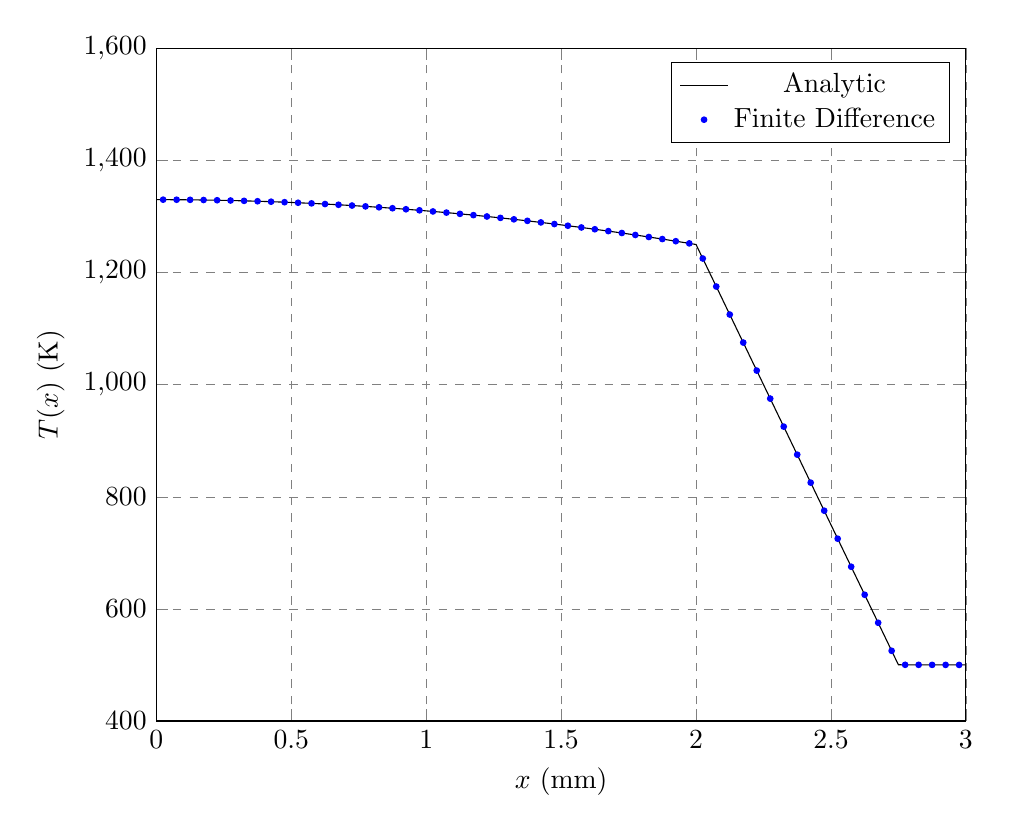
\begin{tikzpicture} \begin{axis}
[scale=1.5,
 xmin=0,    xmax=3,
 ymin=400, ymax=1600,
 grid=major, 
 major grid style={color=gray,line width=0.2pt, dashed},
 xlabel=$x$ (mm),
 ylabel=$T(x)$ (K),
]

\addplot[thin, color=black] coordinates {
 (  0.000 , 1330.250 )
 (  0.025 , 1330.237 )
 (  0.050 , 1330.200 )
 (  0.075 , 1330.137 )
 (  0.100 , 1330.050 )
 (  0.125 , 1329.937 )
 (  0.150 , 1329.800 )
 (  0.175 , 1329.637 )
 (  0.200 , 1329.450 )
 (  0.225 , 1329.237 )
 (  0.250 , 1329.000 )
 (  0.275 , 1328.737 )
 (  0.300 , 1328.450 )
 (  0.325 , 1328.137 )
 (  0.350 , 1327.800 )
 (  0.375 , 1327.437 )
 (  0.400 , 1327.050 )
 (  0.425 , 1326.637 )
 (  0.450 , 1326.200 )
 (  0.475 , 1325.737 )
 (  0.500 , 1325.250 )
 (  0.525 , 1324.737 )
 (  0.550 , 1324.200 )
 (  0.575 , 1323.637 )
 (  0.600 , 1323.050 )
 (  0.625 , 1322.437 )
 (  0.650 , 1321.800 )
 (  0.675 , 1321.137 )
 (  0.700 , 1320.450 )
 (  0.725 , 1319.737 )
 (  0.750 , 1319.000 )
 (  0.775 , 1318.237 )
 (  0.800 , 1317.450 )
 (  0.825 , 1316.637 )
 (  0.850 , 1315.800 )
 (  0.875 , 1314.937 )
 (  0.900 , 1314.050 )
 (  0.925 , 1313.137 )
 (  0.950 , 1312.200 )
 (  0.975 , 1311.237 )
 (  1.000 , 1310.250 )
 (  1.025 , 1309.237 )
 (  1.050 , 1308.200 )
 (  1.075 , 1307.137 )
 (  1.100 , 1306.050 )
 (  1.125 , 1304.937 )
 (  1.150 , 1303.800 )
 (  1.175 , 1302.637 )
 (  1.200 , 1301.450 )
 (  1.225 , 1300.237 )
 (  1.250 , 1299.000 )
 (  1.275 , 1297.737 )
 (  1.300 , 1296.450 )
 (  1.325 , 1295.137 )
 (  1.350 , 1293.800 )
 (  1.375 , 1292.437 )
 (  1.400 , 1291.050 )
 (  1.425 , 1289.637 )
 (  1.450 , 1288.200 )
 (  1.475 , 1286.737 )
 (  1.500 , 1285.250 )
 (  1.525 , 1283.737 )
 (  1.550 , 1282.200 )
 (  1.575 , 1280.637 )
 (  1.600 , 1279.050 )
 (  1.625 , 1277.437 )
 (  1.650 , 1275.800 )
 (  1.675 , 1274.137 )
 (  1.700 , 1272.450 )
 (  1.725 , 1270.737 )
 (  1.750 , 1269.000 )
 (  1.775 , 1267.237 )
 (  1.800 , 1265.450 )
 (  1.825 , 1263.637 )
 (  1.850 , 1261.800 )
 (  1.875 , 1259.938 )
 (  1.900 , 1258.050 )
 (  1.925 , 1256.137 )
 (  1.950 , 1254.200 )
 (  1.975 , 1252.237 )
 (  2.000 , 1250.250 )
 (  2.025 , 1225.250 )
 (  2.050 , 1200.250 )
 (  2.075 , 1175.250 )
 (  2.100 , 1150.250 )
 (  2.125 , 1125.250 )
 (  2.150 , 1100.250 )
 (  2.175 , 1075.250 )
 (  2.200 , 1050.250 )
 (  2.225 , 1025.250 )
 (  2.250 , 1000.250 )
 (  2.275 ,  975.250 )
 (  2.300 ,  950.250 )
 (  2.325 ,  925.250 )
 (  2.350 ,  900.250 )
 (  2.375 ,  875.250 )
 (  2.400 ,  850.250 )
 (  2.425 ,  825.250 )
 (  2.450 ,  800.250 )
 (  2.475 ,  775.250 )
 (  2.500 ,  750.250 )
 (  2.525 ,  725.250 )
 (  2.550 ,  700.250 )
 (  2.575 ,  675.250 )
 (  2.600 ,  650.250 )
 (  2.625 ,  625.250 )
 (  2.650 ,  600.250 )
 (  2.675 ,  575.250 )
 (  2.700 ,  550.250 )
 (  2.725 ,  525.250 )
 (  2.750 ,  500.250 )
 (  2.775 ,  500.225 )
 (  2.800 ,  500.200 )
 (  2.825 ,  500.175 )
 (  2.850 ,  500.150 )
 (  2.875 ,  500.125 )
 (  2.900 ,  500.100 )
 (  2.925 ,  500.075 )
 (  2.950 ,  500.050 )
 (  2.975 ,  500.025 )
 (  3.000 ,  500.000 )
};
\addlegendentry{Analytic};

\addplot[only marks, mark=*, mark size=1pt, color=blue] coordinates {
 (  0.025 , 1330.250 )
 (  0.075 , 1330.150 )
 (  0.125 , 1329.950 )
 (  0.175 , 1329.650 )
 (  0.225 , 1329.250 )
 (  0.275 , 1328.750 )
 (  0.325 , 1328.150 )
 (  0.375 , 1327.450 )
 (  0.425 , 1326.650 )
 (  0.475 , 1325.750 )
 (  0.525 , 1324.750 )
 (  0.575 , 1323.650 )
 (  0.625 , 1322.450 )
 (  0.675 , 1321.150 )
 (  0.725 , 1319.750 )
 (  0.775 , 1318.250 )
 (  0.825 , 1316.650 )
 (  0.875 , 1314.950 )
 (  0.925 , 1313.150 )
 (  0.975 , 1311.250 )
 (  1.025 , 1309.250 )
 (  1.075 , 1307.150 )
 (  1.125 , 1304.950 )
 (  1.175 , 1302.650 )
 (  1.225 , 1300.250 )
 (  1.275 , 1297.750 )
 (  1.325 , 1295.150 )
 (  1.375 , 1292.450 )
 (  1.425 , 1289.650 )
 (  1.475 , 1286.750 )
 (  1.525 , 1283.750 )
 (  1.575 , 1280.650 )
 (  1.625 , 1277.450 )
 (  1.675 , 1274.150 )
 (  1.725 , 1270.750 )
 (  1.775 , 1267.250 )
 (  1.825 , 1263.650 )
 (  1.875 , 1259.950 )
 (  1.925 , 1256.150 )
 (  1.975 , 1252.250 )
 (  2.025 , 1225.250 )
 (  2.075 , 1175.250 )
 (  2.125 , 1125.250 )
 (  2.175 , 1075.250 )
 (  2.225 , 1025.250 )
 (  2.275 ,  975.250 )
 (  2.325 ,  925.250 )
 (  2.375 ,  875.250 )
 (  2.425 ,  825.250 )
 (  2.475 ,  775.250 )
 (  2.525 ,  725.250 )
 (  2.575 ,  675.250 )
 (  2.625 ,  625.250 )
 (  2.675 ,  575.250 )
 (  2.725 ,  525.250 )
 (  2.775 ,  500.225 )
 (  2.825 ,  500.175 )
 (  2.875 ,  500.125 )
 (  2.925 ,  500.075 )
 (  2.975 ,  500.025 )
};
\addlegendentry{Finite Difference};
\end{axis}
\end{tikzpicture}
\caption{Temperature distribution obtained from the finite difference method on the nuclear fuel plate heat conduction example.}
 \label{Fig:ode_finiteDifferenceHeatConduction_temperatureDistributionNuclearFuelPlate}
\end{center}
\end{figure}

To demonstrate the quality of the solution, the following numerical values are used:
\begin{align}
  R_f &= 0.2 \text{ cm}, \nonumber \\
  R_g &= 0.275 \text{ cm}, \nonumber \\
  R_c &= 0.3 \text{ cm}, \nonumber \\
  k_f &= 0.25 \text{ W$\cdot$m$^{-1}\cdot$K$^{-1}$}, \nonumber \\
  k_g &= 0.02 \text{ W$\cdot$m$^{-1}\cdot$K$^{-1}$}, \nonumber \\ 
  k_c &= 20 \text{ W$\cdot$m$^{-1}\cdot$K$^{-1}$}, \nonumber \\
  Q   &= 1 \times 10^7 \text{ W$\cdot$m$^{-3}$}, \nonumber \\
  h   &= 100 \text{ W$\cdot$m$^{-2}\cdot$K$^{-1}$}, \nonumber \\
  T_\infty &= 300 \text{ K}. \nonumber
\end{align}
The problem is solved using a cell-centered finite difference method with a $\Delta x = 0.005$~cm. The results of the finite difference solution are compared with the analytic solution in Fig.~\ref{Fig:ode_finiteDifferenceHeatConduction_temperatureDistributionNuclearFuelPlate}. For this problem, the finite difference solution agrees with the reference analytic solution with the cell-average quantities lining up well within a degree $K$ compared to the analytical solution.
